\documentclass[a4paper,12pt]{book}
\usepackage{a4wide}
\usepackage[T1]{fontenc}
\usepackage{graphicx}
\usepackage{color}
\usepackage{array}
\usepackage{amsmath}
\usepackage{amsfonts}
\usepackage{amssymb}
\usepackage{units}
\usepackage{pgf,tikz}
\usetikzlibrary{arrows}
\usetikzlibrary{babel} % para evitar error con Spanish- babel
\usepackage{url}
\usepackage{hyperref}
\usepackage{animate}
\usepackage{epic}
\usepackage{eepicemu}


\newcommand{\dif}[0]{\text{d}}
\newcommand{\deriv}[2]{\frac{\textrm{d} #1}{\textrm{d} #2}}
\newcommand{\derivsec}[2]{\frac{\text{d}^2 #1}{\text{d} #2^2}}
\newcommand{\dparc}[2]{\frac{\partial #1}{\partial #2}}
\newcommand{\dparcsec}[2]{\frac{\partial^2 #1}{\partial #2^2}}
\newcommand{\Deriv}[2]{\frac{\text{D} #1}{\text{D} #2}}
\newcommand{\mean}[1]{\overline{#1}}
\newcommand{\tens}{\vec{\vec \tau}}
\newcommand{\laplace}{\triangle}
\newcommand{\re}{\text{Re}}
\newcommand{\ma}{\text{Ma}}
\renewcommand{\binom}[2]{\genfrac{}{}{0pt}{}{#1}{#2}}
\newcommand{\rot}{\vec \nabla \times }
\newcommand{\convec}{\left(\vec v \cdot \vec \nabla\right)}

\usepackage[backend=bibtex]{biblatex}
\addbibresource{MFBooks.bib}

%\includeonly{./TeX_files/chapter01-Introduccion/chapter01-Introduccion}

\begin{document}

\author{\bfseries{Robert Castilla} \\
	Dpt. de Mecànica de Fluids}
\title{Mecánica de Fluidos
	\\ {\large Grau de Tecnologies Industrials - ESEIAAT}}
\date{version 1.1 - Septiembre 2024}

\frontmatter
\maketitle
\tableofcontents

\mainmatter

\chapter{Introducción. Propiedades básicas de los fluidos}

\section{Definición de fluido}

Definición corta:


\fbox{\textcolor{red}{\textbf{Material incapaz de resistir esfuerzos tangenciales}}}

\begin{itemize}
	\item \textit{esfuerzo} : Fuerza por unidad de superficie
	
	\item \textit{tangencial} : ni compresión ni dilatación
\end{itemize}


Simplificaci\'on: \textbf{los fluidos son materiales muy f\'acilmente deformables.}

\bigskip

Pero la separaci\'on entre s\'olidos y fluidos no est\'a clara. Hay materiales
que se resiten a una clasificaci\'on sencilla. P.e. : pinturas, pastas, pol\'{\i}meros,
etc ... Ser\'an analizados en detalle en el tema de \textbf{Reolog\'{\i}a.}


A nivel molecular, la diferencia entre l\'{\i}quidos y gases tiene relaci\'on con la magnitud de
la fuerza entre mol\'eculas.


\begin{figure}
	\centering       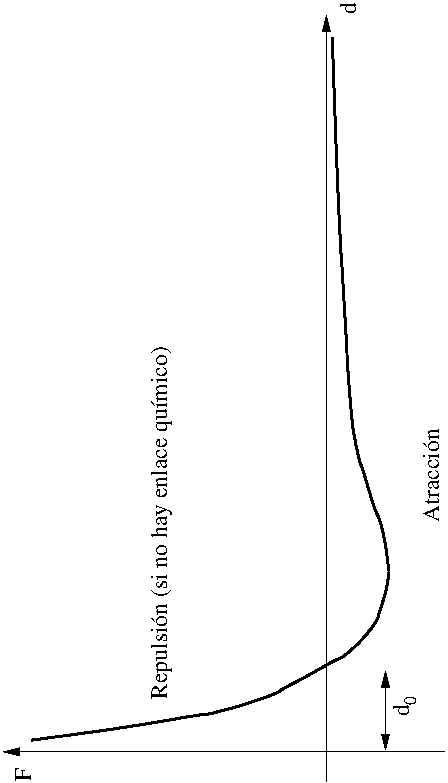
\includegraphics[scale=1,angle=270]{TeX_files/chapter01-Introduccion/fuerzas_molec.pdf}
	\caption{Fuerzas intermoleculares}
	
\end{figure}

En $d_0$, se produce un equilibrio estable.

Para la mayoria de las mol\'eculas, $d_0$ es del orden de  $3-4\cdot10^{-10}$ metros.

Para l\'{\i}quidos, la distancia entre mol\'eculas es, aproximadamente, $d_0$. P.e., para el agua:

$$
\rho \approx 1000 \, \textrm{Kg}/\textrm{m}^3
$$
$$
\textrm{Peso molecular} \approx 0.018 \, \textrm{Kg}/\textrm{mol} \Rightarrow
m = 3.0 \cdot 10^{-26} \, \textrm{Kg}/\textrm{molecula}
$$
$$
V_m = \frac{3.0 \cdot 10^{-26} \, \textrm{Kg}/\textrm{molecula}}{1000 \, \textrm{Kg}/\textrm{m}^3}
=3.0 \cdot 10^{-29} \, \textrm{m}^3
$$
$$
V_m = \frac{4}{3} \pi R^3 \Rightarrow R \approx 1.9 \cdot 10^{-10} \, \textrm{m}
$$

Para los gases, la distancia es mucho mayor (Ejercicio: calcular $d$ para el aire).

As\'{\i}, las fuerzas entre las mol\'eculas de un gas son atractivas y muy d\'ebiles. Estas mol\'eculas
flotan por el espacio sin pr\'acticamente ninguna interacci\'on excepto las colisiones.

\section{Hipótesis del medio continuo}

Todos los materiales est\'an formados por mol\'eculas. Las propiedades del material no estan distribuidas
uniformemente. Si la escala de observaci\'on es lo bastante peque\~na, la composici\'on molecular del material
debe tenerse en cuenta (hablamos entonces de {\em Mec\'anica Estad\'{\i}stica}).

Sin embargo, en {\em Mec\'anica de Fluidos}, se habla normalmente de la densidad, la temperatura, la velocidad,
como una \textcolor{red}{distribuci\'on uniforme de estas propiedades}, sin considerar la naturaleza discreta de la materia. Es
normal hablar de "diferenciales de volumen". Sin embargo, estos diferenciales no son los mismos que los usados
en C\'alculo Infinitesimal. Son volumenes finitos, pero

\begin{itemize}
	\item lo suficientemente grandes como para albergar un n\'umero enorme de mol\'eculas, de forma que las fluctuaciones en las propiedades se anulen entre s\'{\i}, y
	\item lo suficientemente peque\~nos como para que la propiedad pueda ser considerada \em{local}.
\end{itemize}

Batchelor \cite{Batchelor1997} lo describe muy bien con una figura parecida a esta:
\begin{center}
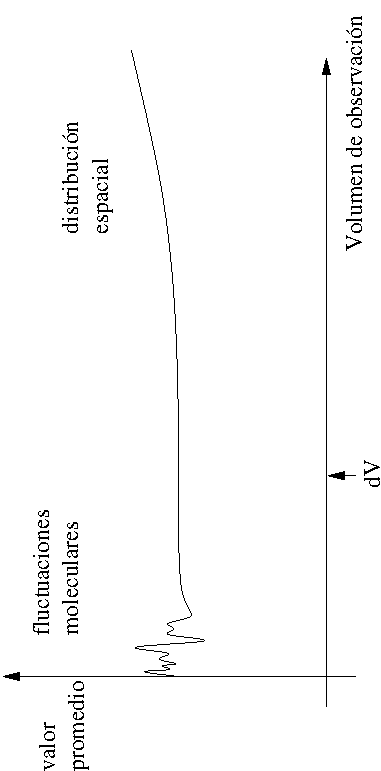
\includegraphics[scale=1,angle=270]{TeX_files/chapter01-Introduccion/difer_vol.pdf}
\end{center}

\section{Propiedades de los fluidos}
\begin{itemize}
	\item \textbf{Propiedades mec\'anicas}
	\begin{itemize}
		\item{\textcolor{red}{densidad - volumen espec\'{\i}fico}}
		$$
		\rho = \frac{m}{V} \qquad ; \qquad \left[\rho\right] = \frac{\textrm{Kg}}{\textrm{m}^3}
		$$
		$$
		v = \frac{1}{\rho} = \frac{V}{m} \qquad ; \qquad \left[v\right] = \frac{\textrm{m}^3}{\textrm{Kg}}
		$$
		\item{\textcolor{red}{M\'odulo de elasticidad} (isot\'ermico)}
		$$
		\beta_T = -v \left(\deriv{p}{v}\right)_T = \rho \left(\deriv{p}{\rho}\right)_T \qquad ; \qquad \left[\beta_T\right] = \textrm{Pa}
		$$
		
		Dado que, \textit{para un gas ideal a temperatura constante}, $\rho \propto p$, tenemos que $\beta_T = p$.
		
		Para una variaci\'on de presi\'on $\Delta p$, la variaci\'on relativa de densidad se puede calcular mediante
		
		$$
		\frac{\Delta \rho}{\rho} = \frac{\Delta p}{\beta_T}
		$$
		
		
		\begin{quotation}
			\textbf{Criterio de compresibilidad} : Todos los fluidos son compresibles, en mayor o menor grado.
			Es importante saber en qu\'e condiciones  un fluido podr\'a ser considerado compresible y cu\'ando no. Supongamos que es considerado compresible si $\frac{\Delta \rho}{\rho} \leq 0.01$. Entonces,
			$$
			\frac{\Delta p}{\beta_T} \lessapprox 0.01.
			$$
			
			Como veremos m\'as adelante, se puede relacionar $\Delta p$ con la velocidad de flujo,
			$$
			\Delta p \sim \frac{1}{2} \rho u^2,
			$$
			de forma que un fluido con velocidad $u$ se puede considerar incompresible si
			$$
			\frac{\rho u^2}{\beta_T} \lessapprox 0.02.
			$$
			
			Como ejemplo, consideremos el aire a presi\'on atmosf\'erica, $ \beta_T = p = 10^5 \,\textrm{Pa}$,
			$\rho \approx 1.2 \,\frac{\textrm{Kg}}{\textrm{m}^3}$.
			
			$$ u^2 \lessapprox \frac{0.02 \beta_T}{\rho} = \frac{0.02 \cdot 10^5}{1.2} = 1.66 \cdot 10^3 \textrm{m}^2/\textrm{s}^2$$
			$$ \Rightarrow u \approx 40 \, \textrm{m/s} $$
			
			\subsection*{Ejercicio} 
			Para el agua, a $20^\circ C$ y presi\'on atmosf\'erica, $\beta_T \approx \unit[2.2\times 10^9]{Pa}$
			y $\rho \approx \unit[1000]{Kg/m^3}$.
			Calcular para qu\'e orden de magnitud de velocidad de flujo el agua debe empezar a considerarse compresible.
		\end{quotation}
		
		\item{\textcolor{red}{Viscosidad}}
		
		Si un fluido fluye en la direcci\'on $x$, de forma ordenada, por capas, aumentando la velocidad en la direcci\'on
		$z$, como muestra la figura,
		
		\begin{center}
			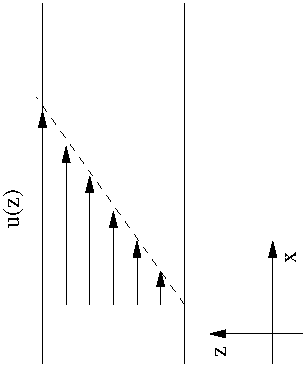
\includegraphics[scale=1,angle=270]{TeX_files/chapter01-Introduccion/u_z.pdf}
		\end{center}
		
		se produce un intercambio de cantidad de movimiento entre capas que tiende a frenar las m\'as r\'apidas y acelerar las m\'as lentas. Es decir, se produce un \textit{esfuerzo tangencial}. En muchos casos, \'este esfuerzo es proporcional al gradiente de velocidades, y a la constante de proporcionalidad se le denomina \textit{\textcolor{red}{viscosidad din\'amica}}, $\mu$. Ésta es la conocida como \textbf{Ley de Newton de la viscosidad}.
		
		\begin{equation}
			\tau = \mu \dparc{u}{z} \qquad ; \qquad \left[\mu\right] = \textrm{Pa}\cdot\textrm{s}
		\end{equation}
		
		
		La \textit{\textcolor{red}{viscosidad cinem\'atica}} se define como
		$$
		\nu = \frac{\mu}{\rho} \qquad ; \qquad \left[\nu\right] = \frac{\textrm{m}^2}{s}
		$$
		
		Ampliaremos el concepto de viscosidad en el tema siguiente.
		
	\end{itemize}
	\item {\textbf{Propiedades termodin\'amicas}}
	
	\textcolor{red}{entalp\'{\i}a}
	$$ h = u + \frac{p}{\rho} = u + p v \qquad ; \qquad \left[h\right] = \left[u\right] = \frac{\textrm{J}}{\textrm{Kg}},
	$$
	
	\textcolor{red}{calor espec\'{\i}fico}
	\begin{eqnarray*}
		c_v = \left(\dparc{q}{T}\right)_v = \dparc{u}{T} & \textrm{a volumen constante} \\
		c_p = \left(\dparc{q}{T}\right)_p = \dparc{h}{T} & \textrm{a presi\'on constante}
	\end{eqnarray*}
	$$
	\left[ c_p \right] = \left[ c_v \right] = \frac{\textrm{J}}{\textrm{Kg}\cdot\textrm{K}}
	$$
	
	La relaci\'on entre ambos coeficientes es:
	$$
	c_p = c_v + \dparc{p v}{T}
	$$
	
	Para un gas perfecto,
	$$ pv = R^\prime T  \Rightarrow \dparc{pv}{T} = R^\prime $$
	$$ \Rightarrow c_p = c_v + R^\prime $$,
	donde $R^\prime = \frac{R}{M}$.
	
	El cociente entre los dos coeficientes se denomina \textit{\textcolor{red}{exponente adiab\'atico}},
	$$
	\gamma = \frac{c_p}{c_v}.
	$$
	
	\textcolor{red}{coeficiente de expansi\'on t\'ermica}
	
	Normalmente,  $\uparrow T \Rightarrow \uparrow v \, (\Rightarrow \downarrow \rho)$.
	
	$$
	\alpha = \frac{1}{v}\deriv{v}{T} = - \frac{1}{\rho} \deriv{\rho}{T} \qquad; \qquad \left[ \alpha \right] = \textrm{K}^{-1}
	$$
	
	Para agua en condiciones normales, $\alpha \approx 1.5\cdot10^{-4} \,\textrm{K}^{-1}$.
	
	Consideremos un gas perfecto, a presi\'on constante,
	$$
	\alpha_p = -\frac{1}{\rho}\left( \dparc{\rho}{T}\right)_p,
	$$
	como $\rho = \frac{p}{R^\prime T}$,
	$$\left(\dparc{\rho}{T}\right)_p = -\frac{p}{R^\prime T^2} \qquad \Rightarrow \alpha_p = \frac{1}{T}$$	
\end{itemize}

\section{Fuerzas sobre fluidos}
\subsection{Fuerzas de superficie}

Act\'uan sobre el contorno de un  volumen determinado de fluido.

Se crean por contacto bien del mismo fluido, un fluido diferente o un s\'olido.

Dada una superficie $\delta \vec S$, y una fuerza superficial $\delta \vec F$ actuando sobre ella, \'esta se
puede descomponer en una componente normal y una componente tangencial.

\begin{center}
	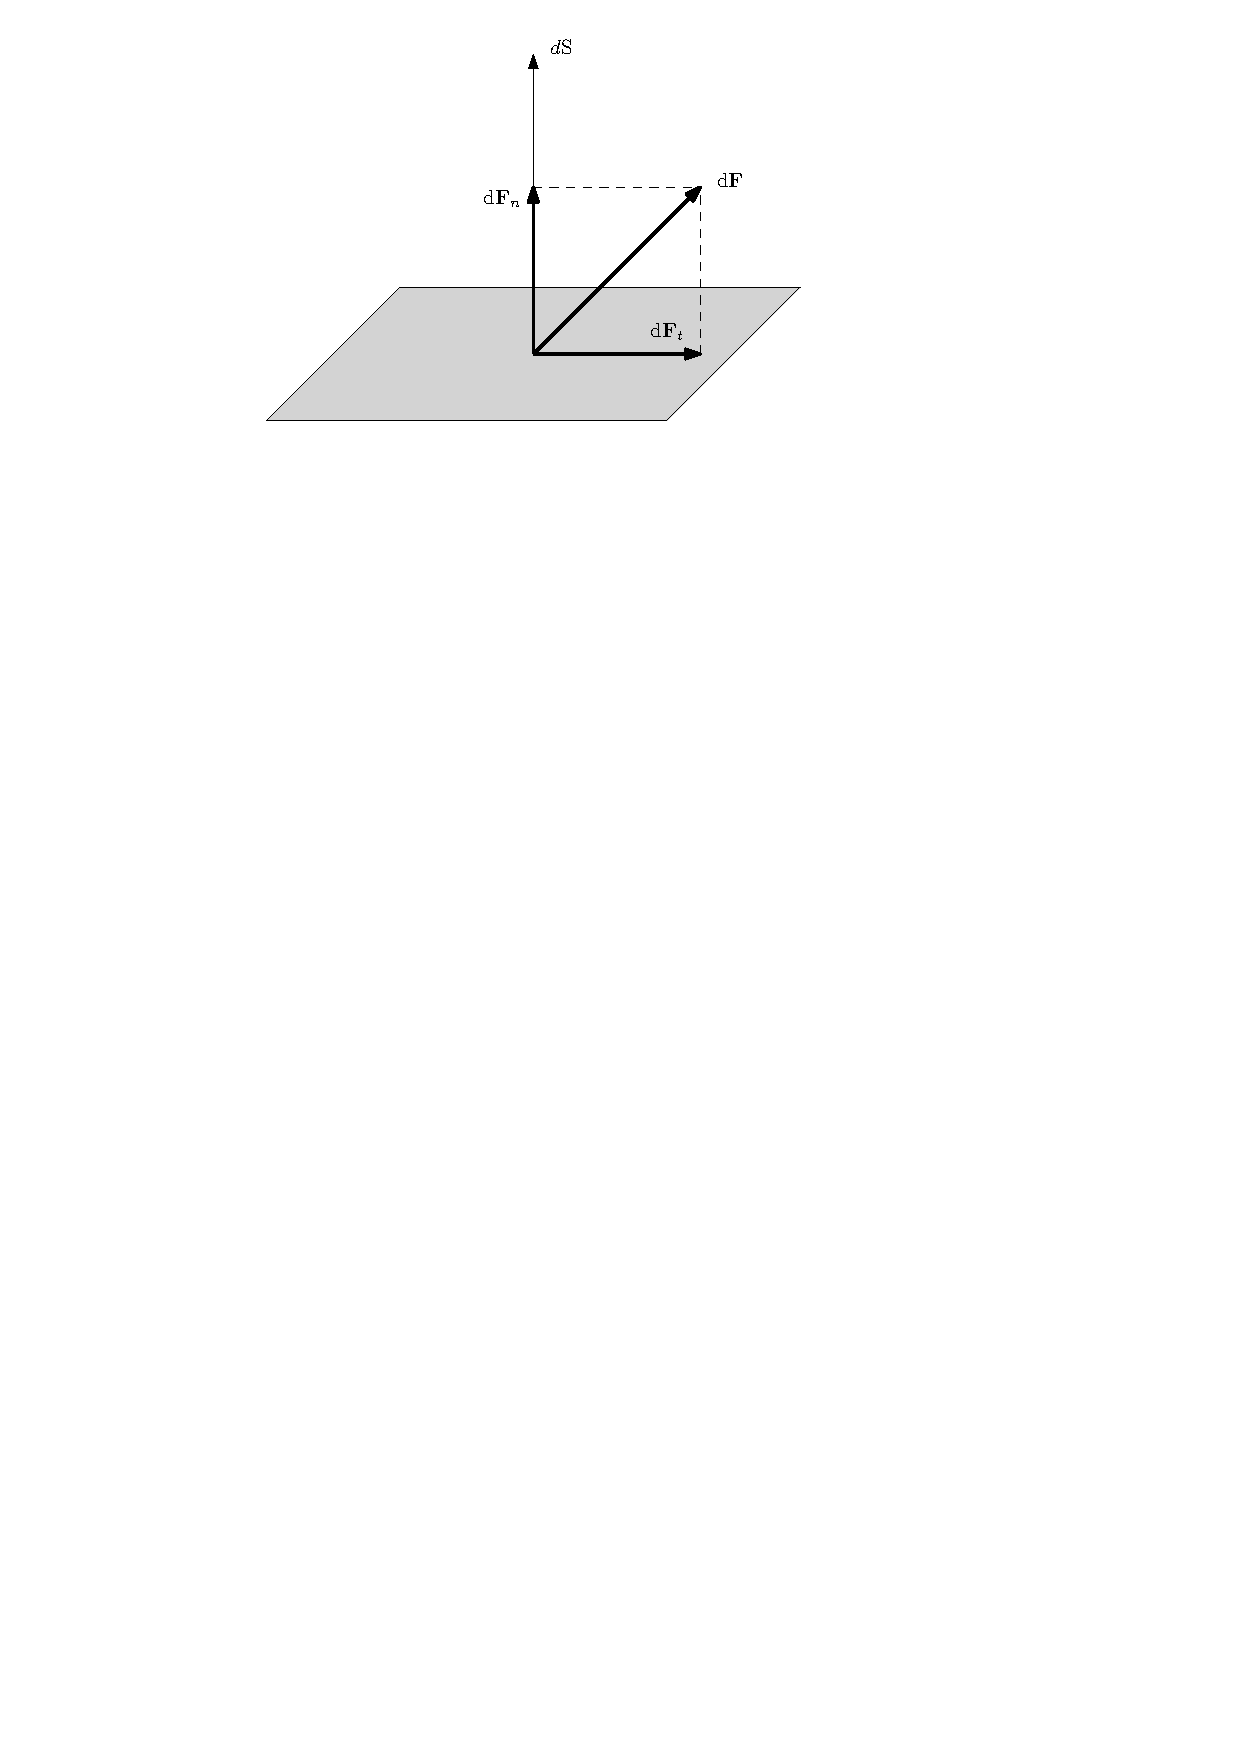
\includegraphics{TeX_files/chapter01-Introduccion/dS.pdf}
\end{center}

Definici\'on de tensi\'on o esfuerzo:

%\begin{center}
	\begin{tabular}{ll}
		\textcolor{blue}{esfuerzo normal} : & \begin{minipage}{10cm}$$\sigma = \lim_{\delta \vec S \rightarrow 0} \frac{\delta \vec F_n}{\delta \vec S}$$\end{minipage} \\
		\textcolor{blue}{esfuerzo tangencial} : & \begin{minipage}{10cm}$$\tau = \lim_{\delta \vec S \rightarrow 0} \frac{\delta \vec F_t}{\delta \vec S}$$ \end{minipage}\\
	\end{tabular}
%\end{center}

\begin{description}
	\item[$\sigma_i$ :] esfuerzo normal aplicado sobre una superficie normal al eje $i$ (y, por lo tanto, paralelo al eje $i$)
	\item[$\tau_{ij}$ :] esfuerzo tangencial aplicado sobre una superficie normal al eje $i$, y en la direcci\'on del eje $j$
\end{description} 

\begin{center}
%	\tikzstyle{isometric}=[x={(0.710cm,-0.410cm)},y={(0cm,0.820cm)},z={(-0.710cm,-0.410cm)}]
\tikzstyle{dimetric} =[x={(0.935cm,-0.118cm)},y={(0cm,0.943cm)},z={(-0.354cm,-0.312cm)}]
\tikzstyle{dimetric2}=[x={(0.935cm,-0.118cm)},z={(0cm,0.943cm)},y={(+0.354cm,+0.312cm)}]
\tikzstyle{trimetric}=[x={(-0.926cm,0.207cm)},y={(0cm,0.837cm)},z={(0.378cm,0.507cm)}]

\begin{tikzpicture}[trimetric]
	\coordinate (O) at (0,0,0);
	\draw[-stealth] (0,0,0) -- (6,0,0) node[above]{$x$};
	\draw[-stealth] (0,0,0) -- (0,6,0) node[above]{$y$};
	\draw[-stealth] (0,0,0) -- (0,0,6) node[above]{$z$};
	\draw[fill=gray!30] (0,0,0) -- (0,4,0) -- (0,4,4) -- (0,0,4)-- cycle;	
	\draw (0,0,0) -- (4,0,0) -- (4,4,0) -- (0,4,0)-- cycle;
	\draw (0,0,0) -- (0,0,4) -- (4,0,4) -- (4,0,0)-- cycle;
	\draw[fill=gray!30] (4,0,0) -- (4,4,0) -- (4,4,4) -- (4,0,4)-- cycle;	
	\draw (0,0,4) -- (4,0,4) -- (4,4,4) -- (0,4,4)-- cycle;
	\draw (0,4,0) -- (0,4,4) -- (4,4,4) -- (4,4,0)-- cycle;
%
	\draw[-stealth,thick] (0,2,2) -- (-1,2,2) node[above ]{$\sigma_x$};
	\draw[-stealth,thick] (0,2,2) -- (0,1,2) node[right]{$\tau_{xy}$};
	\draw[-stealth,thick] (0,2,2) -- (0,2,1) node[above=2mm]{$\tau_{xz}$};
%
	\draw[-stealth,thick] (4,2,2) -- (5,2,2) node[left=2mm]
					{$\sigma_x+\frac{\partial \sigma_x}{x} \textrm{d}x$};
	\draw[-stealth,thick] (4,2,2) -- (4,3,2) node[above left]
					{$\tau_{xy}+\frac{\partial \tau_{xy}}{x} \textrm{d}x$};
	\draw[-stealth,thick] (4,2,2) -- (4,2,3) node[right]
					{$\tau_{xz}+\frac{\partial \tau_{xz}}{x} \textrm{d}x$};
\end{tikzpicture}
\tikzstyle{isometric}=[x={(0.710cm,-0.410cm)},y={(0cm,0.820cm)},z={(-0.710cm,-0.410cm)}]
\tikzstyle{dimetric} =[x={(0.935cm,-0.118cm)},y={(0cm,0.943cm)},z={(-0.354cm,-0.312cm)}]
\tikzstyle{dimetric2}=[x={(0.935cm,-0.118cm)},z={(0cm,0.943cm)},y={(+0.354cm,+0.312cm)}]
\tikzstyle{trimetric}=[x={(-0.926cm,0.207cm)},y={(0cm,0.837cm)},z={(0.378cm,0.507cm)}]

\begin{tikzpicture}[trimetric]
	\coordinate (O) at (0,0,0);
	\draw[-stealth] (0,0,0) -- (6,0,0) node[above]{$x$};
	\draw[-stealth] (0,0,0) -- (0,6,0) node[above]{$y$};
	\draw[-stealth] (0,0,0) -- (0,0,6) node[above]{$z$};
	\draw[fill=gray!30] (0,0,0) -- (0,4,0) -- (0,4,4) -- (0,0,4)-- cycle;	
	\draw (0,0,0) -- (4,0,0) -- (4,4,0) -- (0,4,0)-- cycle;
	\draw (0,0,0) -- (0,0,4) -- (4,0,4) -- (4,0,0)-- cycle;
	\draw[fill=gray!30] (4,0,0) -- (4,4,0) -- (4,4,4) -- (4,0,4)-- cycle;	
	\draw (0,0,4) -- (4,0,4) -- (4,4,4) -- (0,4,4)-- cycle;
	\draw (0,4,0) -- (0,4,4) -- (4,4,4) -- (4,4,0)-- cycle;
%
	\draw[-stealth,thick] (0,2,2) -- (-1,2,2) node[above ]{$\sigma_x$};
	\draw[-stealth,thick] (0,2,2) -- (0,1,2) node[right]{$\tau_{xy}$};
	\draw[-stealth,thick] (0,2,2) -- (0,2,1) node[above=2mm]{$\tau_{xz}$};
%
	\draw[-stealth,thick] (4,2,2) -- (5,2,2) node[left=2mm]
					{$\sigma_x+\frac{\partial \sigma_x}{x} \textrm{d}x$};
	\draw[-stealth,thick] (4,2,2) -- (4,3,2) node[above left]
					{$\tau_{xy}+\frac{\partial \tau_{xy}}{x} \textrm{d}x$};
	\draw[-stealth,thick] (4,2,2) -- (4,2,3) node[right]
					{$\tau_{xz}+\frac{\partial \tau_{xz}}{x} \textrm{d}x$};
\end{tikzpicture}
\end{center}

Sobre el volumen $\text{d} V$ act\'ua una fuerza, debida a los esfuerzos superficiales cuya componente $x$ es
\begin{multline}
	\dif F_x = -\sigma_x  \dif y \dif z + \left(\sigma_x + \dparc{\sigma_x}{x} \dif x\right) \dif y \dif z - \tau_{yx} \dif x \dif z + \left(\tau_{yx} + \dparc{\tau_{yx}}{y}\right) \dif x \dif z \\
	- \tau_{zx} \dif x \dif y + \left(\tau_{zx} + \dparc{\tau_{zx}}{z}\right) \dif x \dif y
	= \dparc{\sigma_x}{x} \dif x \dif y \dif z + \dparc{\tau_{yx}}{y} \dif x \dif y \dif z + \dparc{\tau_{zx}}{z}
	\dif x \dif y \dif z
\end{multline}
De la misma forma:
\begin{eqnarray}
	\dif F_y = \dparc{\sigma_y}{y} \dif x \dif y \dif z + \dparc{\tau_{xy}}{x} \dif x \dif y \dif z + \dparc{\tau_{zy}}{z} \dif x \dif y \dif z \\
	\dif F_z = \dparc{\sigma_z}{z} \dif x \dif y \dif z + \dparc{\tau_{xz}}{x} \dif x \dif y \dif z + \dparc{\tau_{yz}}{y} \dif x \dif y \dif z
\end{eqnarray}

La fuerza por unidad de volumen, debida a los esfuerzos superficiales es entonces
\begin{eqnarray*}
	\vec f = \deriv{\vec F}{V} = \left( \dparc{\sigma_x}{x} + \dparc{\tau_{yx}}{y} + \dparc{\tau_{zx}}{z}\right) \vec \imath \\
	+ \left( \dparc{\tau_{xy}}{x} + \dparc{\sigma_y}{y} +  \dparc{\tau_{zy}}{z} \right) \vec \jmath \\
	+ \left( \dparc{\tau_{xz}}{x}  +  \dparc{\tau_{yz}}{y} + \dparc{\sigma_z}{z} \right) \vec k
\end{eqnarray*}
que se expresa de forma abreviada como
\begin{equation}
	 \vec f = \vec \nabla \vec {\vec \tau}
\end{equation}
donde $\vec {\vec \tau}$ es el \textcolor{red}{tensor de tensiones} (stress tensor)
\begin{equation}
	\vec{\vec{\tau}} =
	\left(
	\begin{array}{ccc}
		\sigma_x & \tau_{xy} & \tau_{xz} \\
		\tau_{yx} & \sigma_y & \tau_{yz} \\
		\tau_{zx} & \tau_{zy} & \sigma_z
	\end{array}\right)
\end{equation}

\subsection{Fuerzas m\'asicas}
Act\'uan a distancia

Son debidas a campos de fuerza (gravitacional, electromagn\'etico, \ldots)

Fluido el\'ectricamente cargado : plasma
\begin{itemize}
	\item Electrohidrodin\'amica
	\item Magnetohidrodin\'amica
\end{itemize}

Caso m\'as com\'un: s\'olo campo gravitacional
$$\vec f_g = \rho \vec g$$

\subsection{Fuerzas lineales (tensi\'on superficial)}
En la interfase de separaci\'on entre dos l\'iquidos reside una cantidad de energ\'{\i}a, correspondiente
a la interacci\'on entre moleculas muy pr\'oximas a la superficie de separaci\'on

Esta energ\'{\i}a es proporcional al \'area de la interfase.
\begin{equation}
	 E_s = \sigma S
\end{equation} 

El par\'ametro $\sigma$ recibe el nombre de \textcolor{blue}{tensi\'on superficial} y tiene unidades de fuerza por
unidad de longitud. Esta fuerza es tangente a la superficie, y normal a la l\'{\i}nea de aplicaci\'on.

El valor de $\sigma$ depende de la naturaleza de los materiales que separa la interfase y de su estado termodin\'amico.

P.e. para la interfase entre agua y aire a $20^\circ C$, $\sigma~=~72.8\cdot10^{-3}~\text{N/m}$


\begin{center}
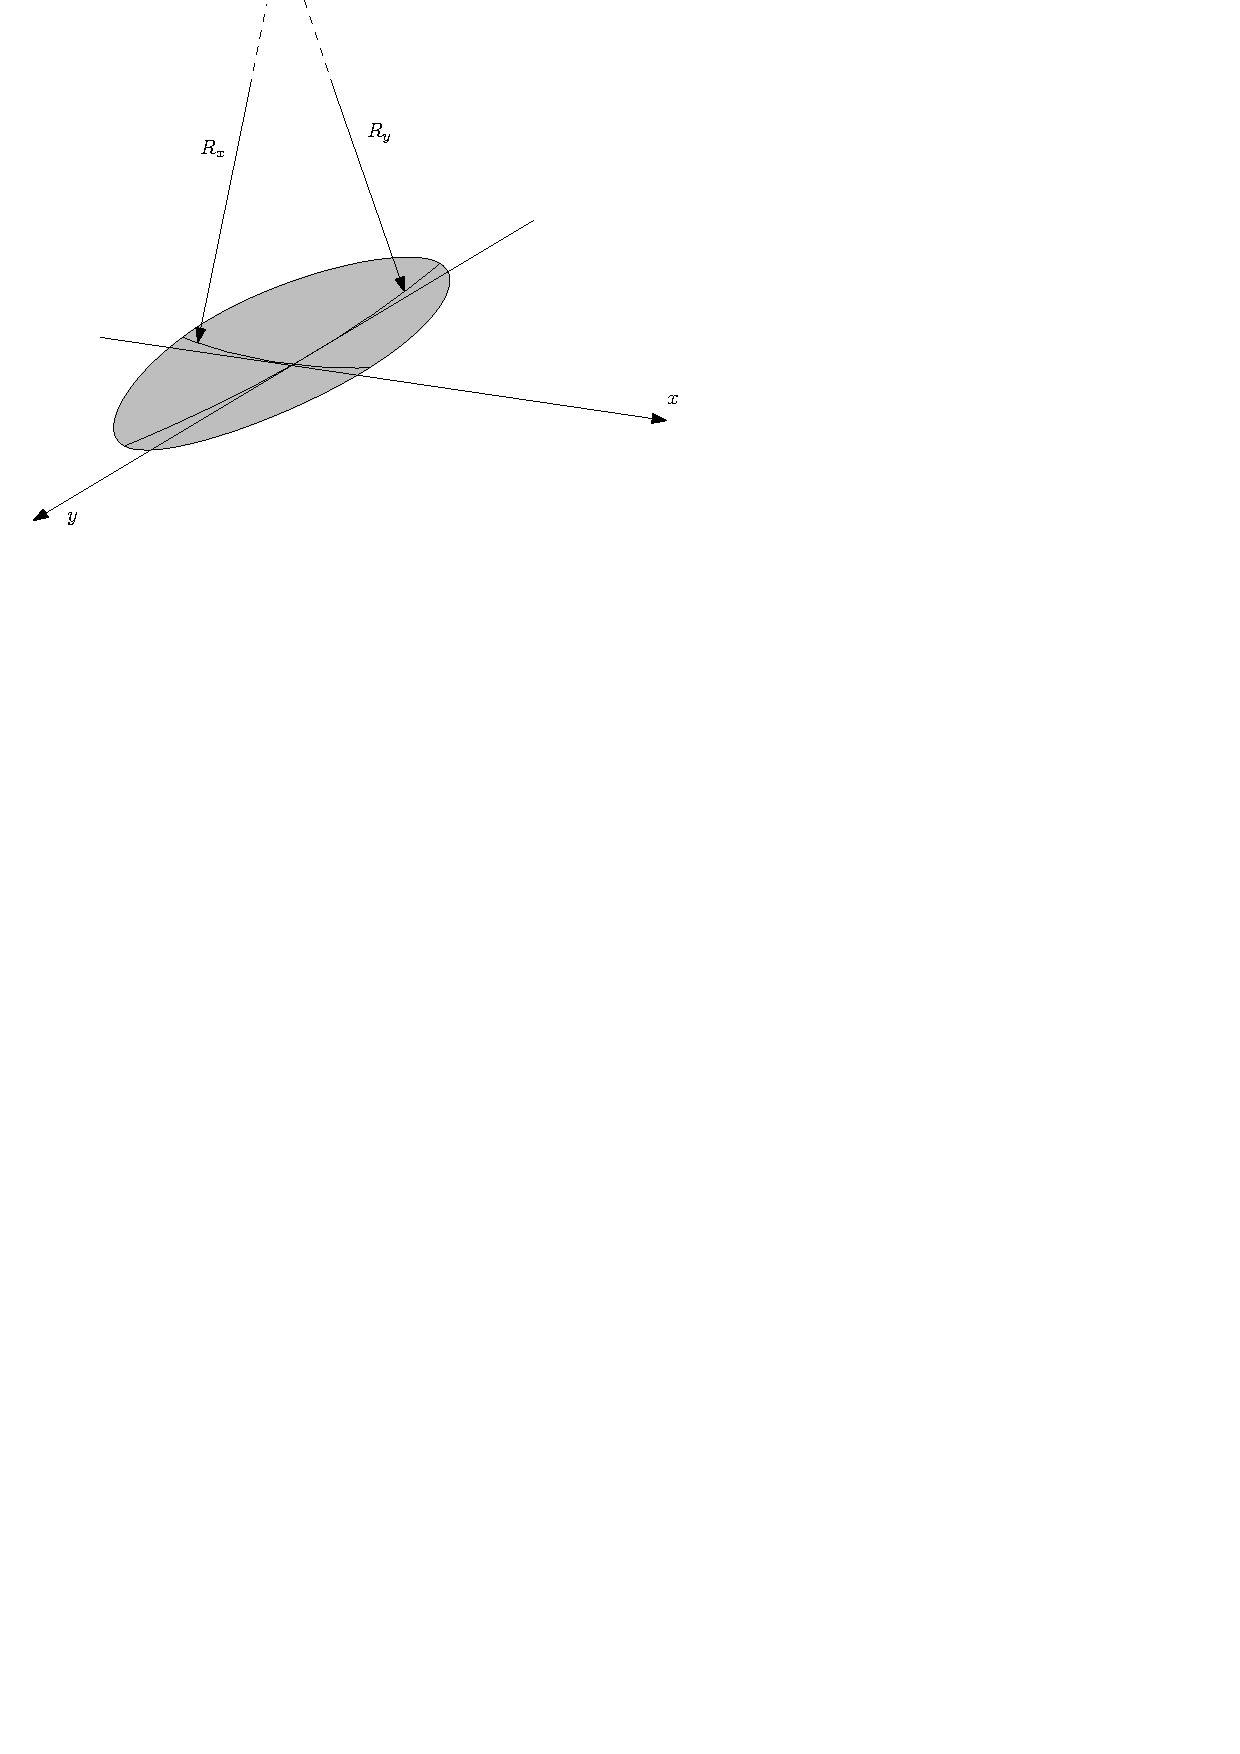
\includegraphics{TeX_files/chapter01-Introduccion/YoungLaplace}
\end{center}
Se puede demostrar (ver \cite{Batchelor1997}) que la tensi\'on provocada en la superfice es equivalente a una diferencia
de presi\'on, como indica la \href{https://es.wikipedia.org/wiki/Ley_de_Laplace}{\textbf{ley de Young-Laplace}}
\begin{equation}
	\Delta p = \sigma\left(\frac{1}{R_x}+\frac{1}{R_y}\right)
\end{equation}


Si los dos radios de curvatura son iguales, ($R_x=R_y=R$, casquete esférico), esta expresión se reduce a 
 
\begin{equation}
	\Delta p = \frac{2\sigma}{R}
\end{equation}

Consideramos el caso de tres fluidos (p.e. una gota de aceite en una superficie de agua)
\begin{center}
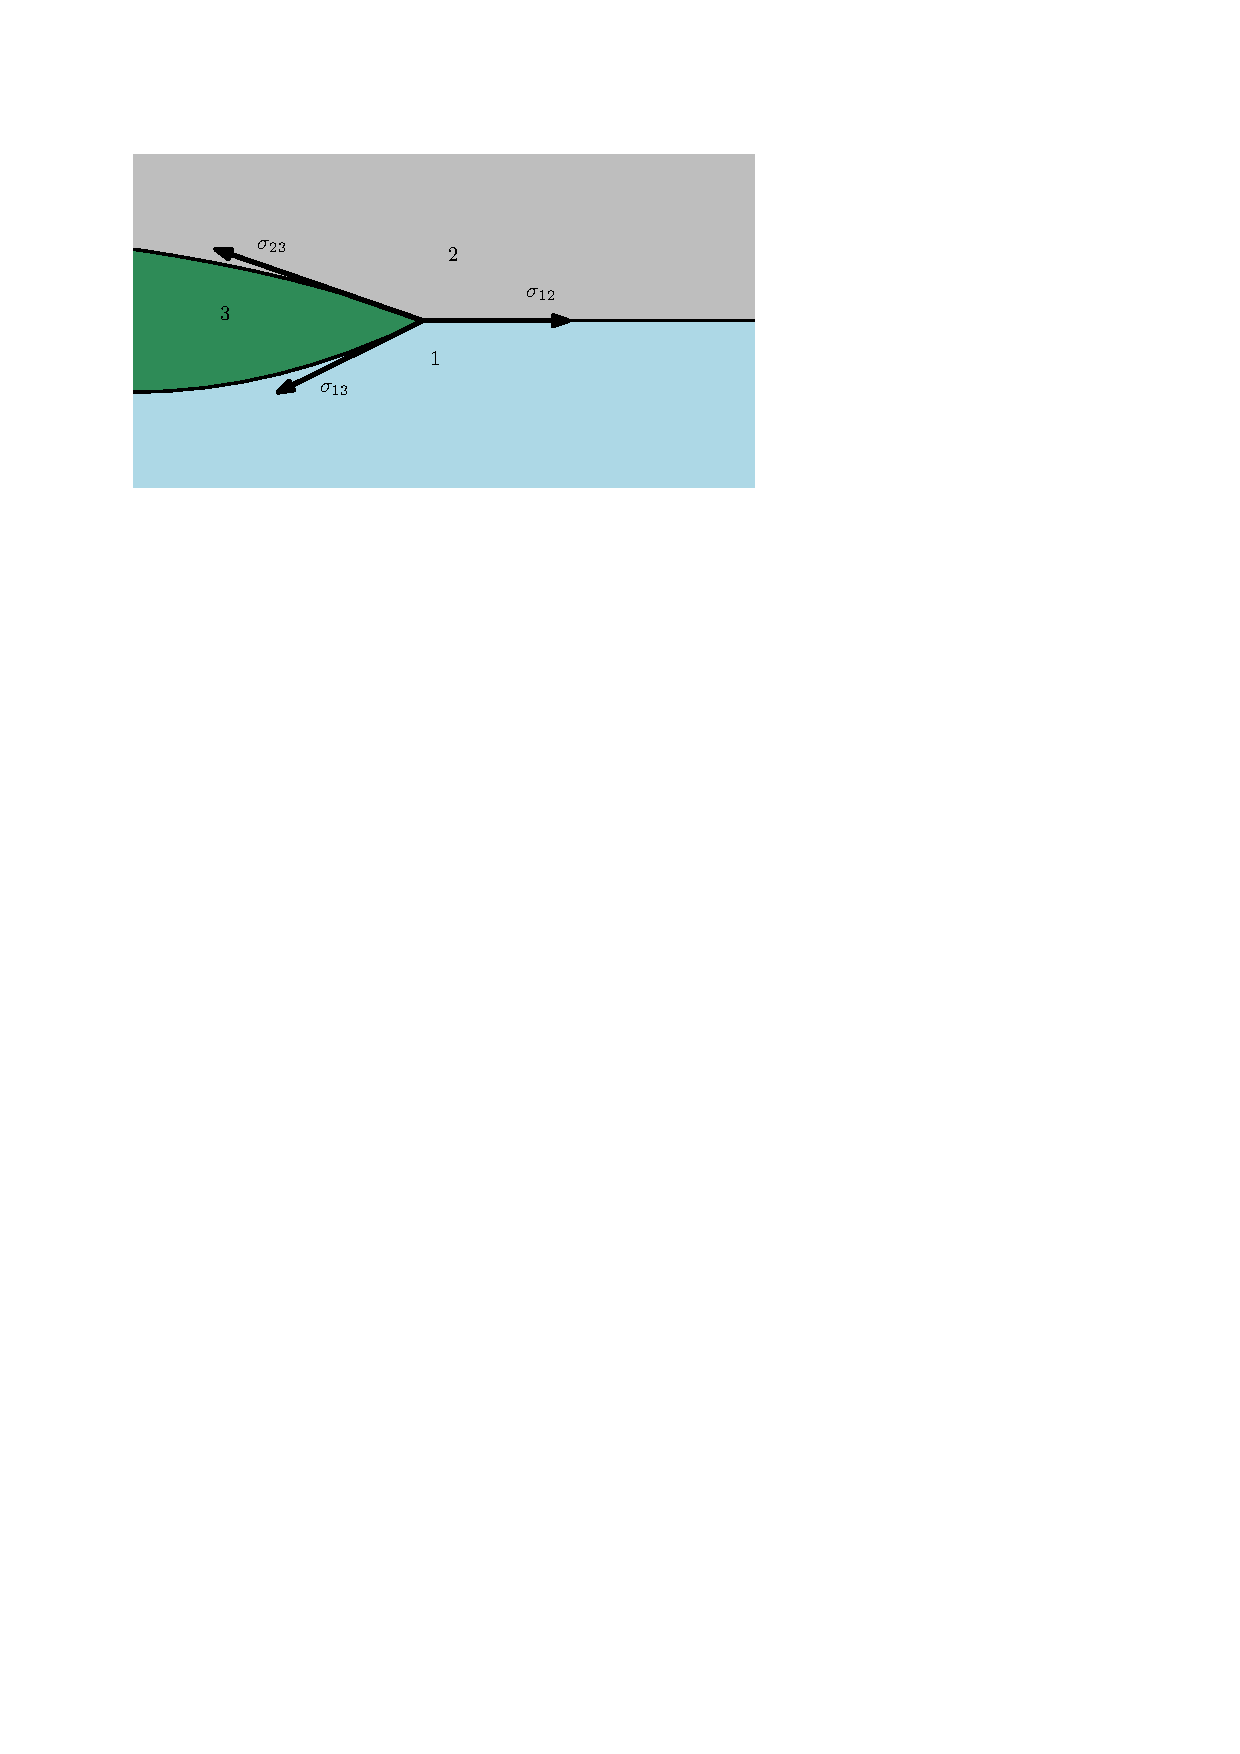
\includegraphics{TeX_files/chapter01-Introduccion/tresFluidos}
\end{center}
Si el m\'odulo de una de las tensiones es mayor que la suma de los m\'odulos de las otras dos, este sistema nunca
puede llegar al equilibrio, y el fluido se expandir\'a de forma indefinida hasta llegar al equilibrio, o tener
un grosor de tama\~no molecular.

Si uno de los materiales es un s\'olido,
\begin{center}
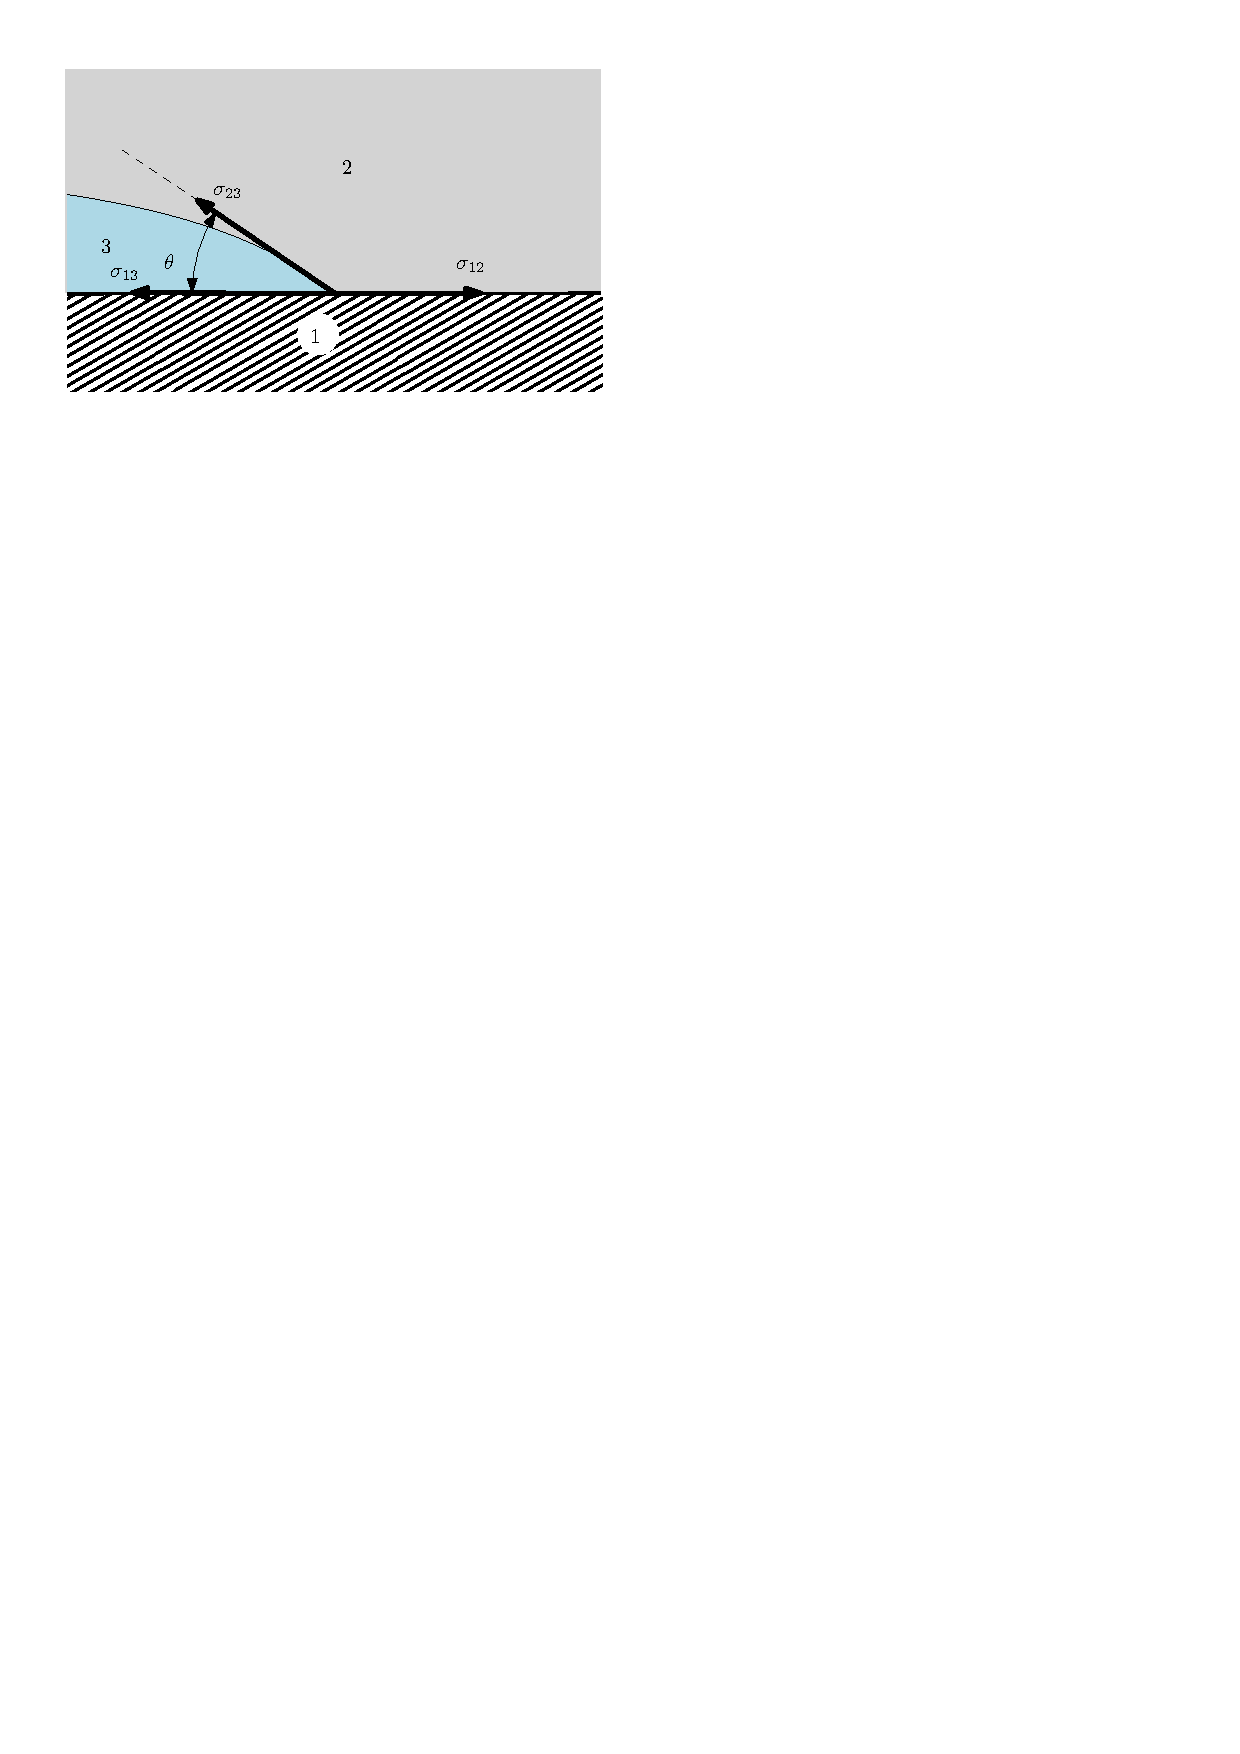
\includegraphics{TeX_files/chapter01-Introduccion/dosysolido}
\end{center}
se llega al equilibrio para
$$ \sigma_{12} = \sigma_{31} + \sigma_{23} \cos{\theta}$$
Se considera que cuanto menor es $\theta$, m\'as "moja" el fluido sobre la superficie del s\'olido.

\subsection*{Ejemplo:}
L\'{\i}quido en contacto con pared plana vertical
\begin{center}
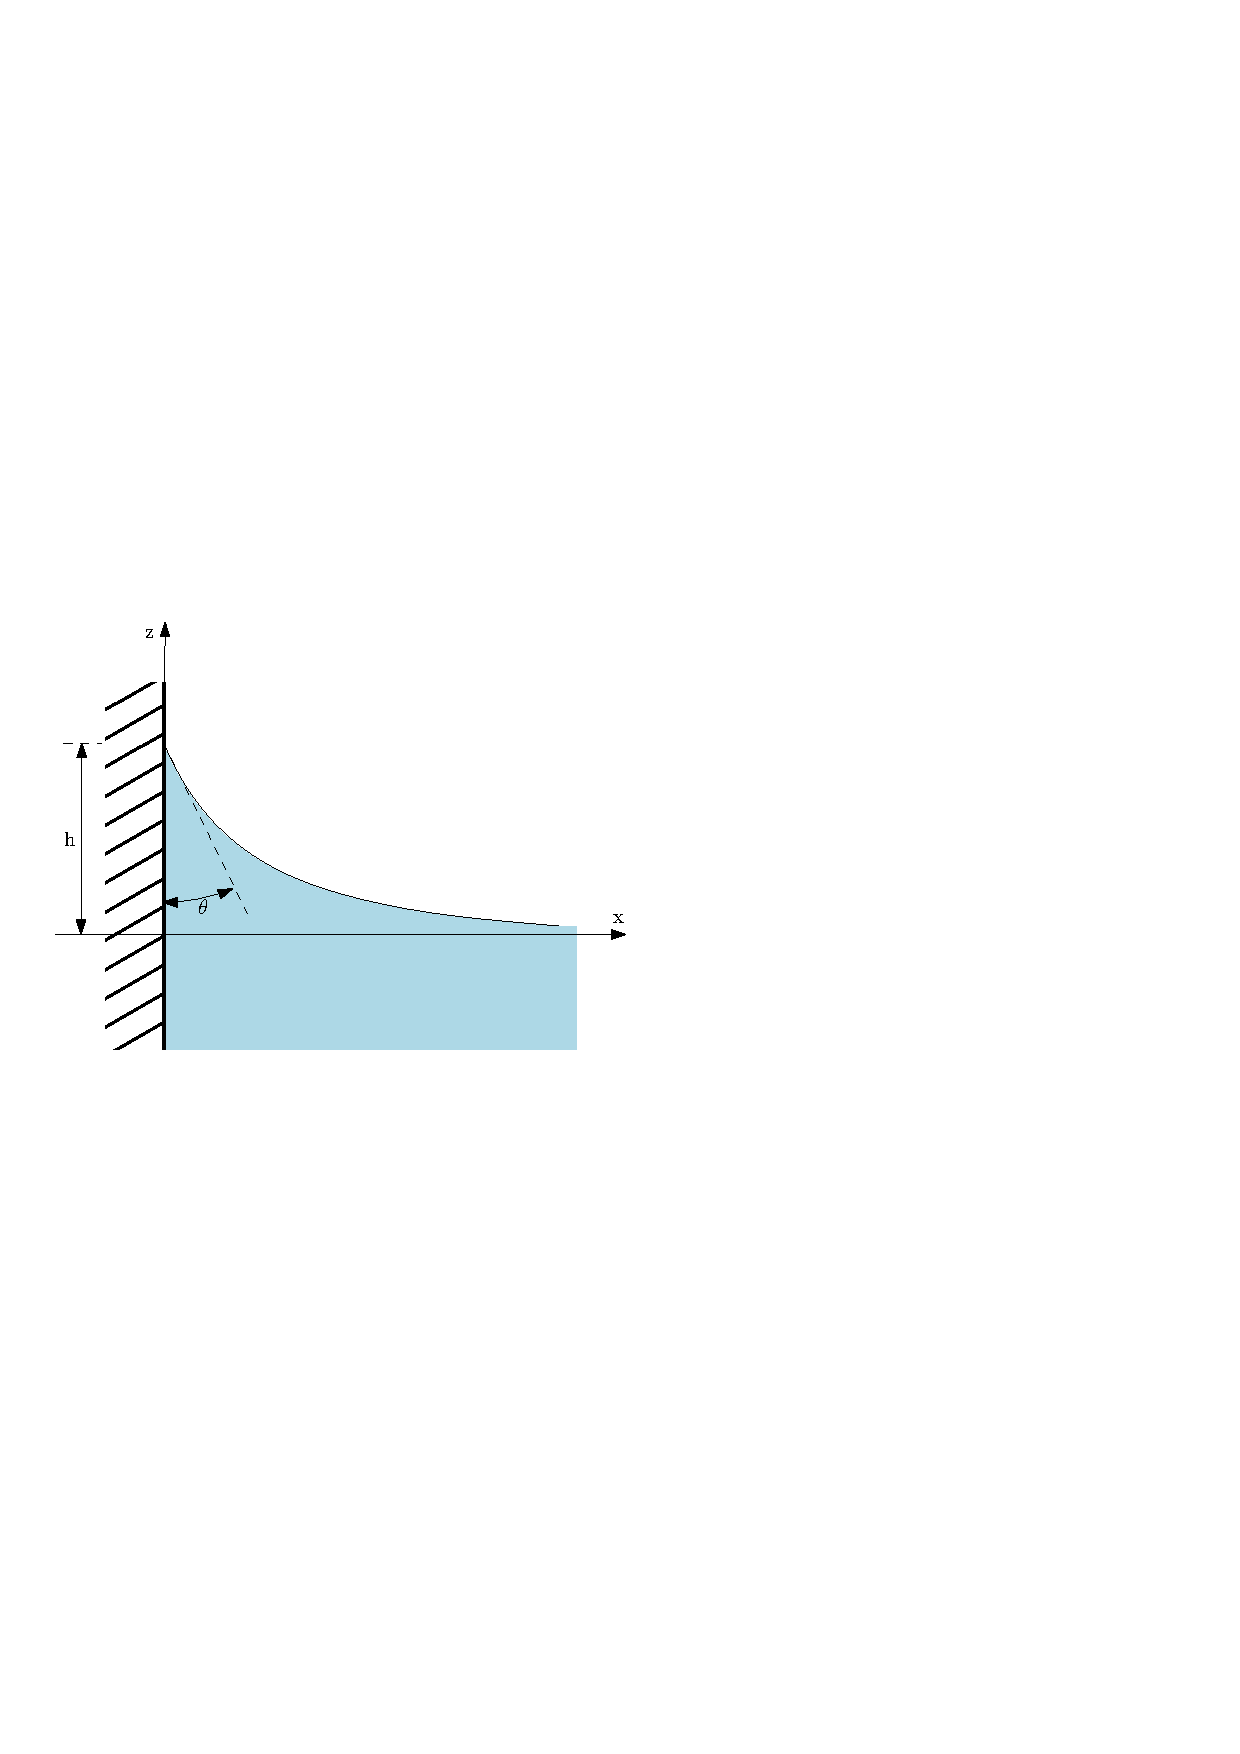
\includegraphics{TeX_files/chapter01-Introduccion/pared.pdf}
\end{center}
Forma de la interficie: $z=\zeta(x)$

En un cierto punto de la interficie, la tensi\'on superficial tiene que ser tal que compense la presi\'on de la columna de fluido. Como veremos m\'as adelante, esta es $\rho g z$, de forma que
$$
\rho g z = \sigma \frac{1}{R_1}
$$
$$
\rho g \zeta = \sigma \frac{\zeta''}{\left( 1 + \zeta'^2\right)^\frac{3}{2}}
$$
Integrando se obtiene
$$
\frac{1}{2}\frac{\rho g}{\sigma}\zeta^2 + \frac{1}{\left(1+\zeta'^2\right)^\frac{1}{2}} = K
$$
Muy lejos de la pared, se cumple que $\zeta=\zeta'=0$, de forma que $K = 1$

Por otro lado, en $x=0$, se tiene (ver figura) $\zeta=h$ y $\zeta'=-\frac{1}{\tan \theta}$, de forma que
$$
h = d \sqrt{2\left(1-\sin \theta \right)}
$$
donde $d^2=\frac{\sigma}{\rho g}$.
\chapter{Hidrostática}

\section{Ecuación fundamental de la fluidostática}

\textbf{Fluido en reposo}: No hay esfuerzos tangenciales, y la única
fuerza superficial es la presión.

Equilibrio estático: 

\begin{equation}
\vec{f}_{m}-\vec{\nabla}p=0
\end{equation}


Según el calculo diferencial, 
\[
\vec{\nabla}\times\left(\vec{\nabla}\phi\right)=0\quad\forall\phi\text{ escalar}
\]

\[
\Rightarrow\vec{\nabla}\times\vec{f_{m}}=0.
\]
 $\Rightarrow\vec{f}_{m}$ ha de ser un \emph{campo conservativo}.

\[
\dif p=\vec{f}_{m}\cdot\dif\vec{r}
\]
 Integrando sobre un determinado camino, 
\[
p\left(\vec{r}\right)=p\left(\vec{r}_{0}\right)+\int_{\vec{r}_{0}}^{\vec{r}}\vec{f}_{m}\cdot\dif\vec{r}
\]
 Nos permite calcular la presión en cualquier punto $\vec{r}$ conociendo
el valor en un punto de referencia $\vec{r}_{0}$ y el campo de fuerzas
$\vec{f}_{m}$.

Si $\vec{f}_{m}$ es conservativo 
\[
\vec{f}_{m}=-\rho\vec{\nabla}U
\]
 y, entonces, 
\[
\vec{\nabla}p=-\rho\vec{\nabla}U
\]

Si $\rho$ varia de forma arbitraria, no existen soluciones para la
ecuación , y no es posible llegar al equilibrio, $\rightarrow$ \textcolor{blue}{corrientes
convectivas}

La ecuación sólo admite soluciones cuando $\rho$ es únicamente función
de la presión, o bien es constante (fluido incompresible). 
\[
p+\rho U=cte
\]

$\rightarrow$ \textcolor{blue}{Principio de Pascal}

Hidrostática en el campo de la gravedad

\[
\vec{f}_{m}=\rho\vec{g},
\]
 con 
\[
\vec{g}=-g\vec{k}\qquad\text{donde }g=9.81\,\frac{\textrm{m}}{\textrm{s}^{2}}
\]
 y 
\[
U=gz
\]



Superficies isobáricas (superficies de igual presión), incluida la
superficie libre de los líquidos, horizontales. %

\[
\vec{\nabla}p=-\rho g\vec{k}\Rightarrow\left\{ \begin{aligned}\dparc{p}{x} & =0\\
\dparc{p}{y} & =0\\
\dparc{p}{z} & =-\rho g
\end{aligned}
\right.
\]
%

La presión es únicamente función de la coordenada $z$.

\[
\deriv{p}{z}=-\rho\,g\Rightarrow\,p_{2}-p_{1}
\]

\[
=-\int_{z_{1}}^{z_{2}}\rho\,g\,\dif z
\]
%

\subsection*{Actividad 1:}
\noindent\begin{minipage}[t]{1\columnwidth}%
\begin{itemize}
\item ¿A cuántos metros de columna de agua corresponden la presión atmosférica?
\item Si el aire fuese incompresible, con la densidad que tiene a nivel
del mar, ¿cuál debería ser la altura de la atmósfera para tener la
misma presión?
\end{itemize}
%
\end{minipage}

\section{Presión atmosférica}

La presión atmosférica disminuye con la altura. Dado que el aire es
un gas, su densidad disminuye, en general, cuando disminuye la presión,
por lo que también es menor cuando aumentamos la altura.

Necesitamos información sobre la variación de $\rho$ con $z$, o
bien con $p$.

Opción: aire gas ideal 
\[
\rho=\frac{pM}{RT}\quad\textnormal{con}\,M=28.9\,\textnormal{g/mol}.
\]
 
\begin{equation}
\Rightarrow\,\frac{\dif p}{p}=-\frac{Mg}{RT}\dif z\label{eq:general}
\end{equation}



Sin considerar la variación de $g$ con la altura: 
\begin{itemize}
\item \textcolor{blue}{Atmósfera isoterma:} 
\[
\int_{p_{0}}^{p}\frac{\dif p}{p}=-\int_{0}^{z}\frac{Mg}{RT}\dif z
\]
 
\[
\ln\frac{p}{p_{0}}=-\frac{Mg}{RT}z=-\frac{\rho_{0}g}{p_{0}}z
\]
 
\begin{equation}
\Rightarrow\boxed{p=p_{0}\exp\left(-\frac{\rho_{0}g}{p_{0}}z\right)=p_{0}\exp\left(-\frac{z}{\alpha}\right)}\label{eq:isotermica}
\end{equation}
 donde 
\[
\alpha=\frac{p_{0}}{\rho_{0}g}
\]
\end{itemize}
Valores normales: 
\[
\left.\begin{aligned}\rho_{0} & =1.292\,\text{Kg}/\text{m}^{3}\\
g & =9.80665\,\text{m}/\text{s}^{2}\\
p_{0} & =760\,\text{mmHg}=101328\,\text{Pa}
\end{aligned}
\right\} \rightarrow\alpha=7997.35\,\text{m}\approx8000\,\text{m}
\]



\begin{itemize}
\item \textcolor{blue}{Atmósfera adiabática:} 
\[
\frac{p}{\rho^{\gamma}}=\frac{p_{0}}{\rho_{0}^{\gamma}}\qquad\text{con}\qquad\gamma=\frac{c_{p}}{c_{v}}=1.4\qquad\text{para aire}
\]
\end{itemize}
\[
\dif p=-g\rho\dif z=-\rho_{0}\left(\frac{p}{p_{0}}\right)^{\frac{1}{\gamma}}g\dif z
\]
 
\[
\Rightarrow\frac{\dif p}{p^{\frac{1}{\gamma}}}=-\frac{\rho_{0}}{p_{0}^{\frac{1}{\gamma}}}g\dif z
\]

\[
\int_{p_{0}}^{p}\frac{\dif p}{p^{\frac{1}{\gamma}}}=\int_{0}^{z}-\frac{\rho_{0}}{p_{0}^{\frac{1}{\gamma}}}g\dif z=-\frac{\rho_{0}}{p_{0}^{\frac{1}{\gamma}}}gz
\]


\[
\Rightarrow\frac{1}{-\frac{1}{\gamma}+1}\left.p^{-\frac{1}{\gamma}+1}\right]_{p_{0}}^{p}=-\frac{\rho_{0}}{p_{0}^{\frac{1}{\gamma}}}gz
\]

\[
\Rightarrow\frac{\gamma}{\gamma-1}\left[p^{\frac{\gamma-1}{\gamma}}-p_{0}^{\frac{\gamma-1}{\gamma}}\right]=-\frac{\rho_{0}}{p_{0}^{\frac{1}{\gamma}}}gz
\]

\[
\Rightarrow p^{\frac{\gamma-1}{\gamma}}-p_{0}^{\frac{\gamma-1}{\gamma}}=\frac{1-\gamma}{\gamma}\frac{\rho_{0}}{p_{0}^{\frac{1}{\gamma}}}gz
\]

\begin{equation}
\Rightarrow\boxed{\left(\frac{p}{p_{0}}\right)^{\frac{\gamma-1}{\gamma}}=1+\frac{1-\gamma}{\gamma}\frac{z}{\alpha}}\label{eq:adiabatica}
\end{equation}


\begin{itemize}
\item \textcolor{blue}{Atmósfera estándar:}
\end{itemize}
En realidad, la temperatura media de la atmósfera disminuye de forma
casi lineal con la altura 
\[
T=T_{0}-Bz
\]
 hasta una altura aproximada de 11000 metros (región conocida como
\textit{troposfera}). Los valores de $T_{0}$ (la temperatura a nivel
del mar) y $B$ (\textit{gradiente térmico}) varían no sólo según
el día sino también a lo largo del mismo día. Los valores estándar
usados por convenio son 
\begin{eqnarray*}
T_{0} & = & 15^{\circ}C=288.16\textnormal{K}\\
B & = & 0.0065\textnormal{K/m}
\end{eqnarray*}



\subsection*{Actividad 2:}
Integrar la ecuación (\ref{eq:general}) con esta distribución de
temperatura para obtener 
\begin{equation}
p=p_{0}\left(1-\frac{Bz}{T_{0}}\right)^{\frac{Mg}{RB}}
\end{equation}

El valor del exponente para aire es 
\[
\frac{Mg}{RB}=5.26
\]

Después de la troposfera, la temperatura se mantiene constante hasta
unos 20000 metros para empezar a aumentar de forma gradual.

Hay que tener siempre en cuenta que esta atmósfera estándar es un
valor promediado. 

\section{Fuerza de un fluido estático sobre una superficie}

\subsection{Cálculo de la fuerza}


\begin{center}
\resizebox{0.8\textwidth}{!}{\input{TeX_files/chapter02-Hidrostatica/superficie.pdftex_t}}
\par\end{center}


\[
F=\int_{S}\dif F=\int_{S}(p_{0}+\rho\,g\,h)\dif S==\int_{S}(p_{0}+\rho\,g\,y\,\sin\theta)\dif S
\]

\[
\Rightarrow\;F=p_{0}\,S+\rho\,g\,\sin\theta\int_{S}y\dif S
\]

\begin{description}
\item [{$\int_{S}y\dif S$}] : momento de primer orden de la superficie
$S$ respecto el eje $x$ $\rightarrow$ coordenada $y_{C}$ del centroide
$C$ de la forma
\end{description}
\[
y_{C}\,S=\int_{S}y\dif S\,\Rightarrow\;F=(p_{0}+\rho\,g\,y_{C}\,\sin\theta)S=(p_{0}+\rho\,g\,h_{C})S
\]

\fbox{%
\noindent\parbox[c]{1\textwidth}{%
 La fuerza ejercida sobre una superficie totalmente sumergida se puede
calcular \textbf{imaginando} que la presión que actúa es constante
en toda la superficie e igual al valor en el centroide. %
}}


\subsection{Coordenadas del punto de aplicación}


Momento de la fuerza $\vec{F}$ respecto el eje $x$: 
\[
y_{cp}F=\int_{S}y\dif F=\int_{S}y(p_{0}+\rho\,g\,y\,\sin\theta)\dif S=p_{0}\int_{S}y\dif S+\rho\,g\,\sin\theta\int_{S}y^{2}\dif S
\]
 
\[
\Rightarrow y_{cp}F=\int_{S}y\dif F=p_{0}\,y_{C}\,S+\rho\,g\,\sin\theta I_{xx}
\]
 donde $I_{xx}$ es el momento de segundo orden de la superficie $S$
respecto el eje $x$.

Nuevo sistema de coordenadas $(\xi,\eta,\zeta)$, paralelo a $(x,y,z)$
pero con origen en el centroide $C$. 
\[
I_{xx}=I_{\xi\xi}+y_{C}^{2}\,S\qquad\text{(T. de Steiner)}
\]

\[
\Rightarrow y_{cp}=y_{C}+\frac{I_{\xi\xi}}{\left(y_{C}+\frac{p_{0}}{\rho\,g\,\sin\theta}\right)S}
\]


Para $x_{cp}$: 
\[
\int_{S}x\dif F=\int_{S}x(p_{0}+\rho\,g\,y\,\sin\theta)\dif S=p_{0}\int_{S}x\dif S+\rho\,g\,\sin\theta\int_{S}xy\dif S
\]
 
\[
\Rightarrow\int_{S}x\dif F=p_{0}\,x_{C}\,S+\rho\,g\,\sin\theta I_{xy}
\]
 
\[
I_{xy}=I_{\xi\eta}+x_{C}\,y_{C}\,S\qquad\text{(T. de Steiner)}
\]
 
\[
\Rightarrow x_{cp}=x_{C}+\frac{I_{\xi\eta}}{\left(y_{C}+\frac{p_{0}}{\rho\,g\,\sin\theta}\right)S}
\]



Normalmente, $p_{0}$ (en general, la presión atmosférica) actúa por
igual en las dos caras de la superficie, 
\begin{align*}
F & =\rho\,g\,h_{C}\,S\\
x_{cp} & =x_{C}+\frac{I_{\xi\eta}}{y_{C}\,S}\\
y_{cp} & =y_{C}+\frac{I_{\xi\xi}}{y_{C}\,S}
\end{align*}

Dado que $I_{\xi\xi}$ es, por definición, una cantidad siempre positiva,
el centro de presiones se encuentra siempre por debajo del centroide.


\subsection{Fuerza sobre una superficie curva totalmente sumergida}


\begin{center}
\resizebox{!}{5cm}{\input{TeX_files/chapter02-Hidrostatica/superficie_curva.pdftex_t}}
\par\end{center}

 
\[
\begin{aligned}F_{x} & =-\int_{S}(p_{0}+\rho\,g\,h)\dif S_{x}\\
F_{y} & =-\int_{S}(p_{0}+\rho\,g\,h)\dif S_{y}
\end{aligned}
\]
 

Si proyectamos la superficie $S$ sobre los planos $x=0$ y $y=0$,
obtenemos $S_{x}$ y $S_{y}$, y podemos calcular $F_{x}$ y $F_{y}$,
así como sus puntos de aplicación.

$F_{z}$ resulta ser igual al peso total de fluido que se encuentra
\emph{por encima} de la superficie curva. La linea de acción de $F_{z}$
pasa por el centro de gravedad de la columna de fluido que hay sobre
la superficie.

Las expresiones anteriores son válidas únicamente para fluidos con
densidad constante. Si el fluido está estratificado, de forma que
hay un \textit{gradiente de densidad}, positivo hacia la dirección
vertical negativa, los cálculos se complican.


\subsection*{Actividad 3:}
Calcula la fuerza, y su punto de aplicación, que hace un embalse de agua de 50
metros de profundidad y 200 metros de ancho sobre la pared, vertical,
de la presa.


\section{Principio de Arquímedes}

\fbox{%
	\parbox{1\textwidth}{%
%\begin{quotation}
	\emph{Todo cuerpo sumergido, completa o parcialmente,
		en un fluido experimenta
		un empuje dirigido verticalmente hacia arriba, con magnitud igual al peso del
		fluido desalojado y cuya  linea de acci\'on pasa por el centro de gravedad
		del fluido desalojado}
%\end{quotation} %
}}


\begin{minipage}{0.4\textwidth}
	\begin{center}
		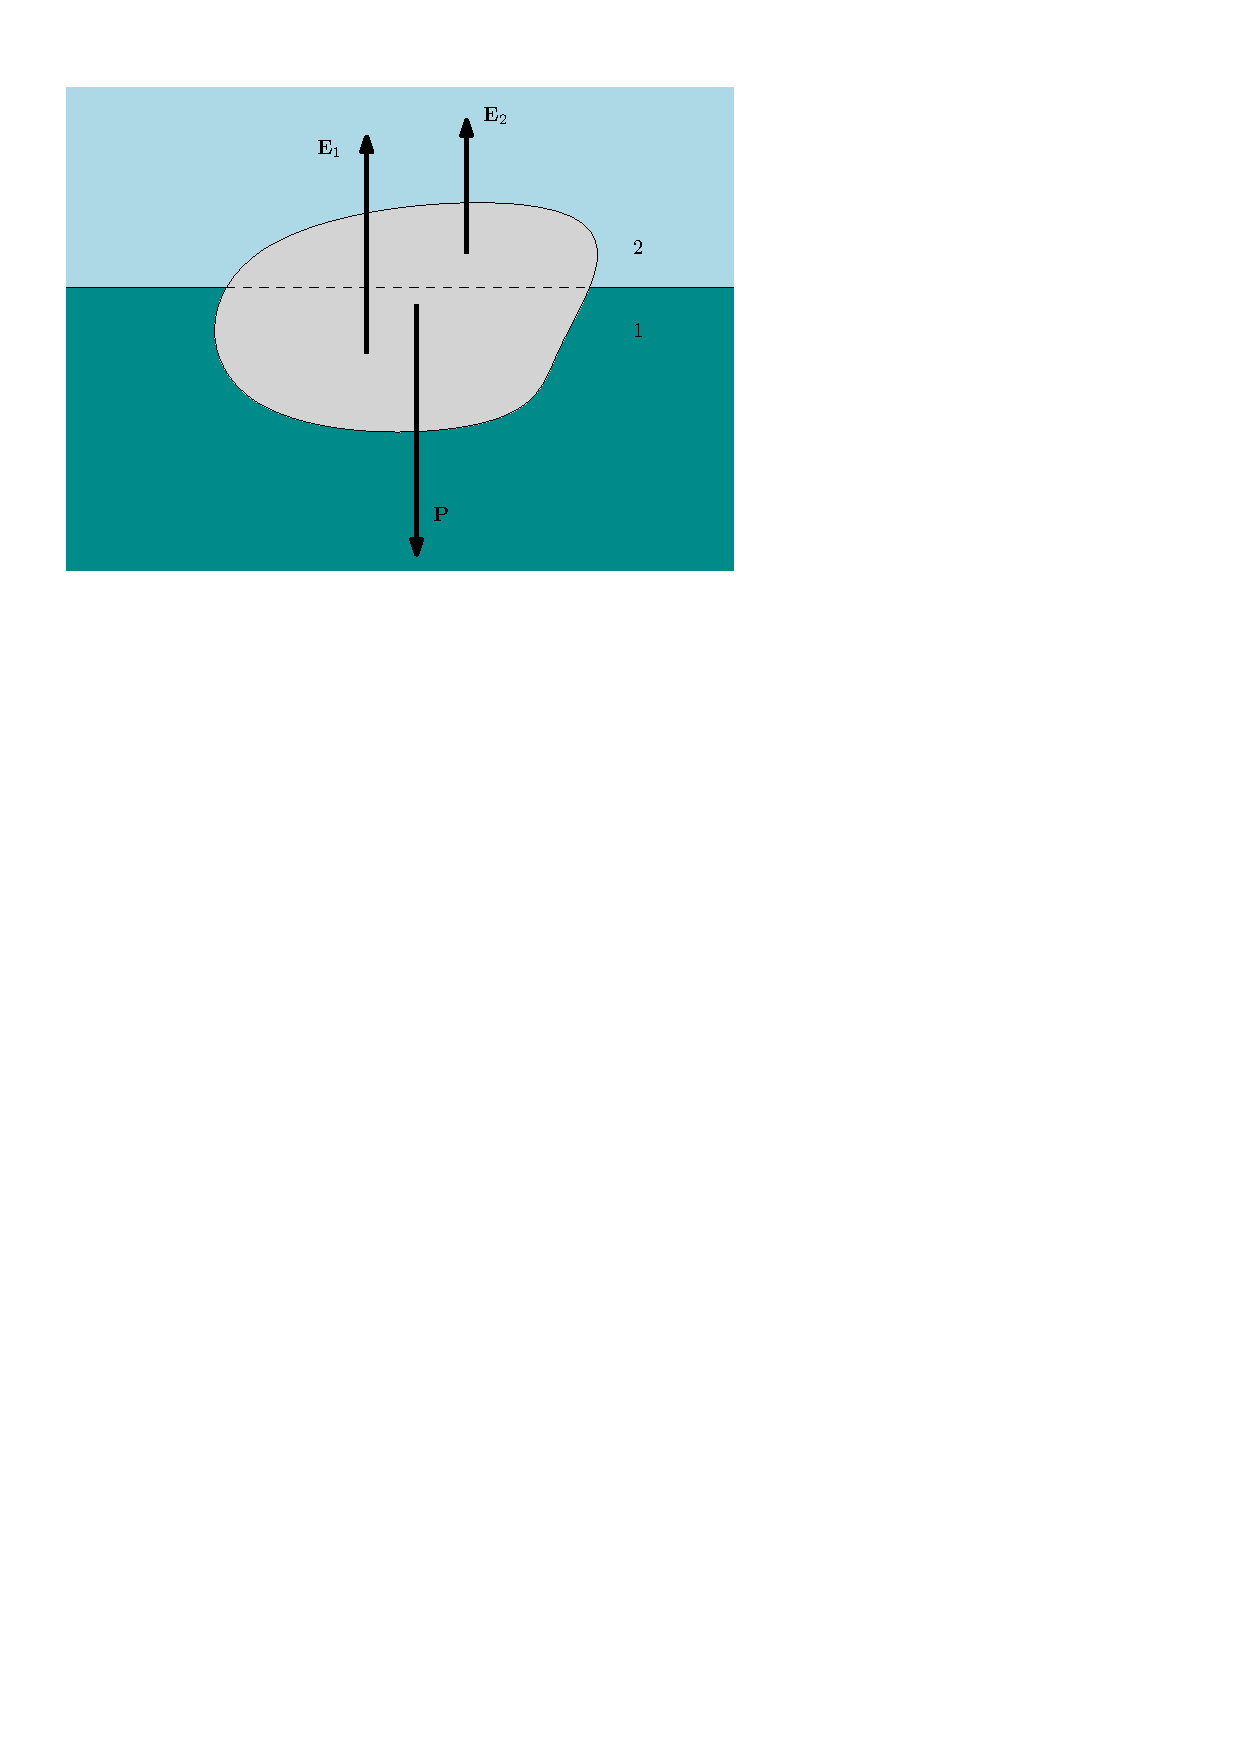
\includegraphics[width=\textwidth]{TeX_files/chapter02-Hidrostatica/arquimedes}
	\end{center}
\end{minipage}
\begin{minipage}{0.5\textwidth}
	Las lineas de acci\'on de las fuerzas de empuje y el peso no
	tienen porqu\'e coincidir, y, en este caso, se producen pares de fuerzas.
	\begin{description}
		\item[\textcolor{blue}{carena}] volumen del fluido desalojado
		\item[\textcolor{blue}{centro
			de carena} o \textcolor{blue}{centro de empuje}] centro de gravedad del fluido desalojado
	\end{description}
\end{minipage}


	El principio de Arquímedes no es, en realidad, un principio. Se puede deducir en cualquier caso simplemente calculando la integral de la presión sobre la superficie que limita el cuerpo.
	
	También se puede obervar que es la resta del peso de la columna de fluido sobre la superficie superior y sobre la superficie inferior.
	
\begin{center}
	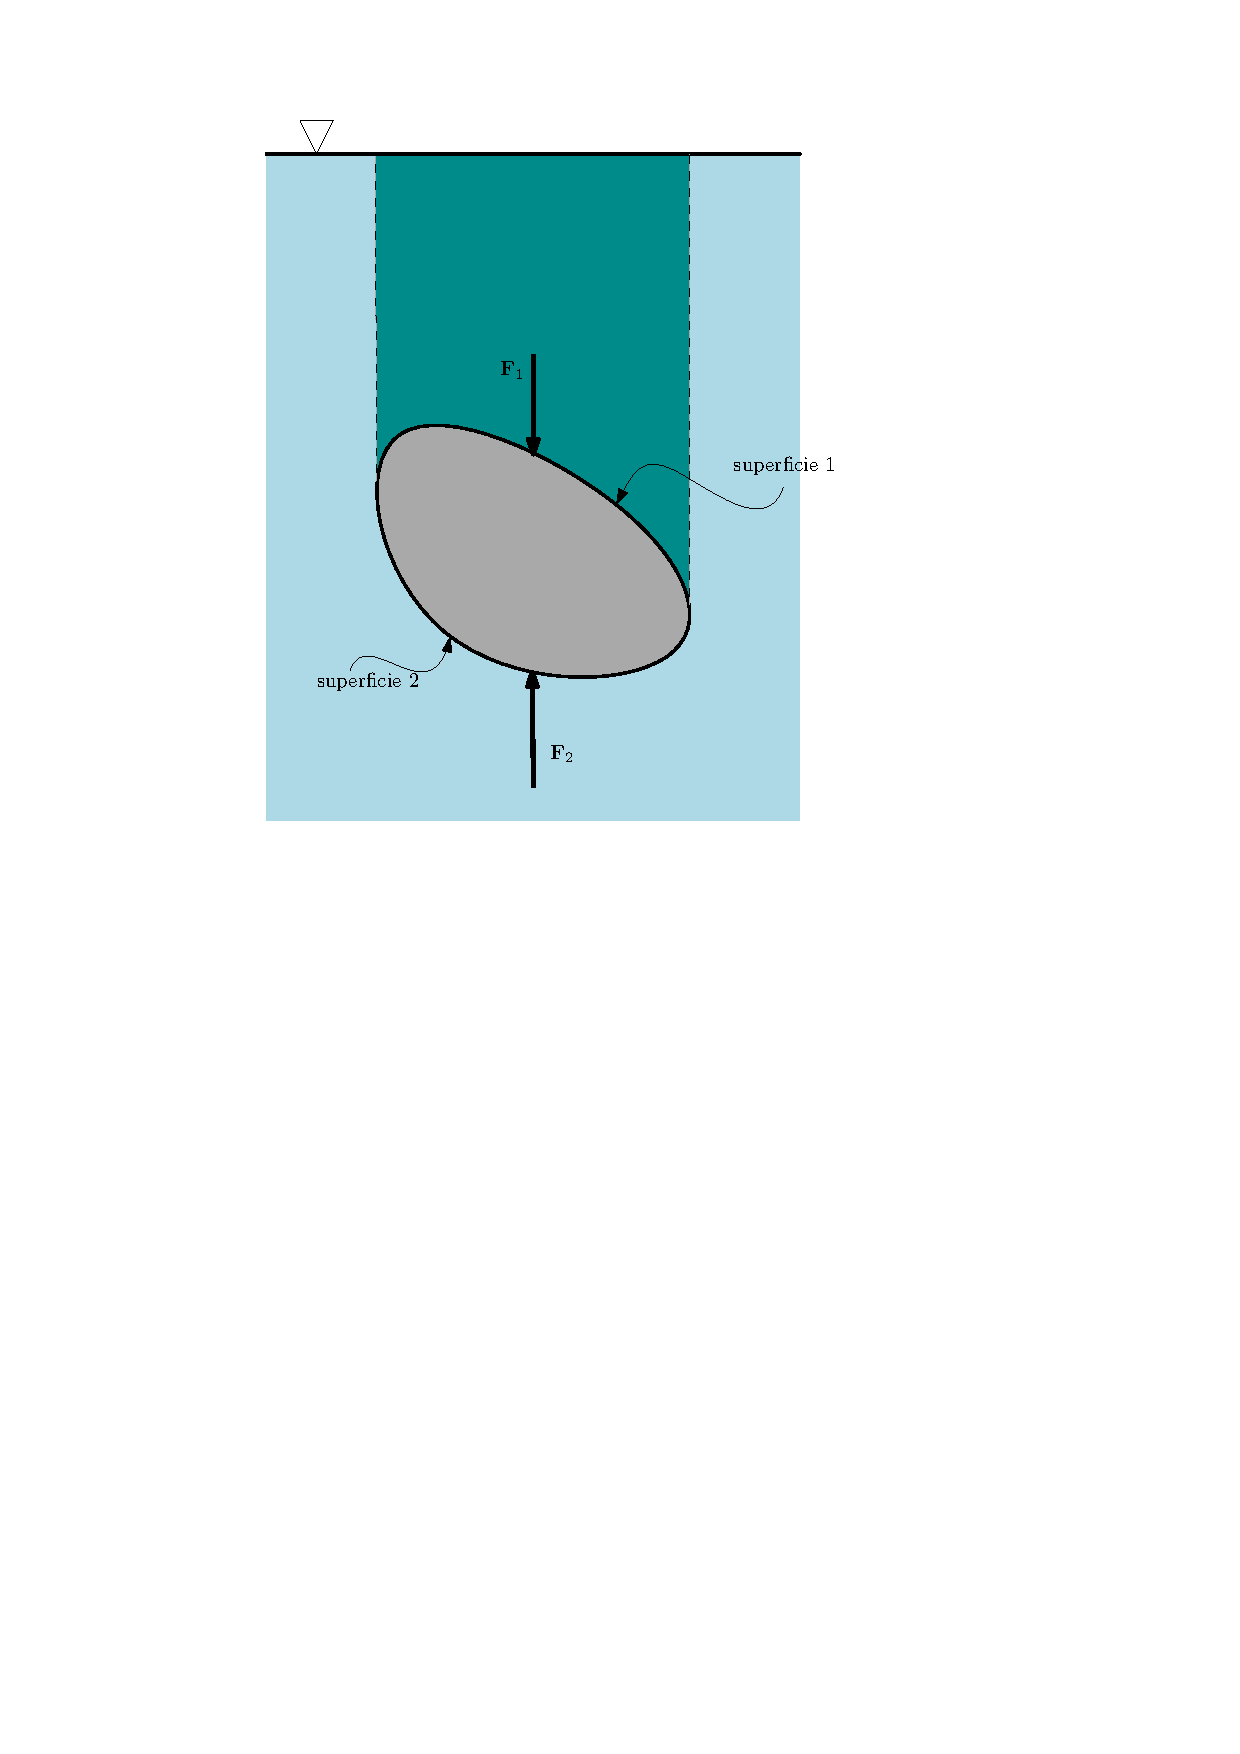
\includegraphics[width=0.5\columnwidth]{TeX_files/chapter02-Hidrostatica/arquimedes2}
\end{center}
\section{Segunda ley de Arquímedes}


	La segunda ley de Arqu\'imedes dice que \emph{un cuerpo que flota desaloja su propio peso de fluido}. 
	
	Se puede comprender observando que en la figura, el recipiente con solo fluido y el que tiene fluido y cuerpo flotando, \textbf{deben pesar lo mismo}. Pregunta: ?`C\'omo sabemos que pesan lo mismo?


	\begin{center}
		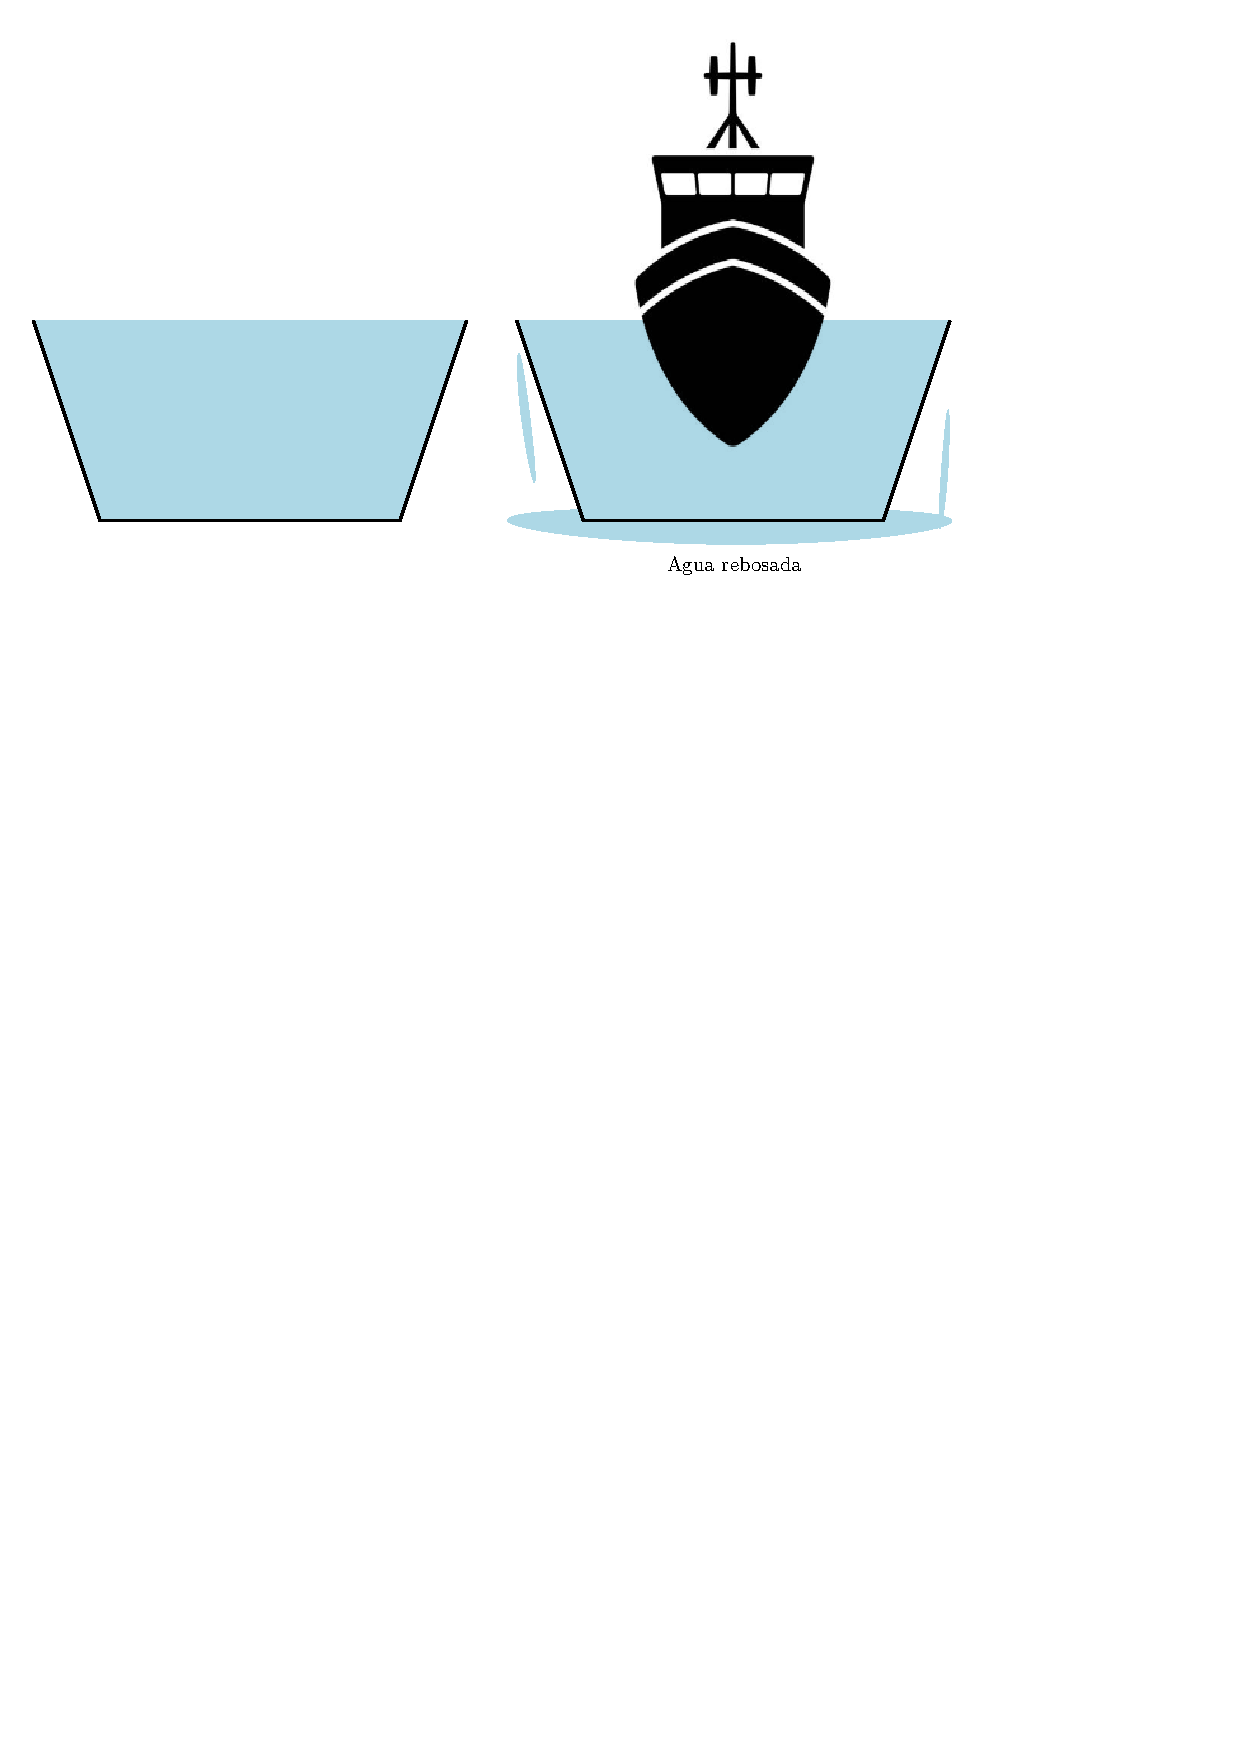
\includegraphics[width=0.75\columnwidth]{TeX_files/chapter02-Hidrostatica/arquimedes1}
	\end{center}


\section{Estabilidad}

Para un cuerpo sumergido, el centro de gravedad puede ser diferente del centro de empuje, y esto produce un momento que puede ser restaurador (equilibrio estable) o de vuelco (equilibrio inestable)

\begin{center}
	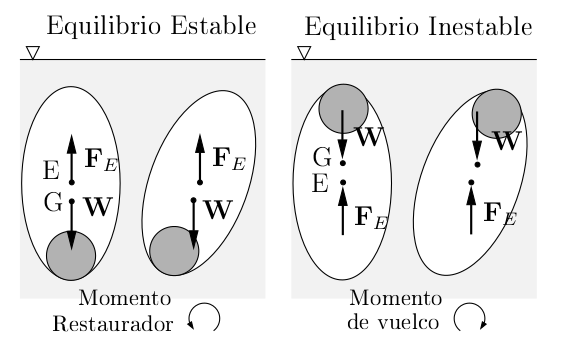
\includegraphics[width=0.7\linewidth]{TeX_files/chapter02-Hidrostatica/estabilidad1}
\end{center}

%\begin{center}
%	\includegraphics[width=0.7\columnwidth]{estab1.png}
%	% estab1.png: 996x491 pixel, 72dpi, 35.14x17.32 cm, bb=
%\end{center}


Para un cuerpo flotante, es m\'as complicado, ya que la posici\'on del centro de empuje var\'ia


Equilibrio estable 
\begin{center}
	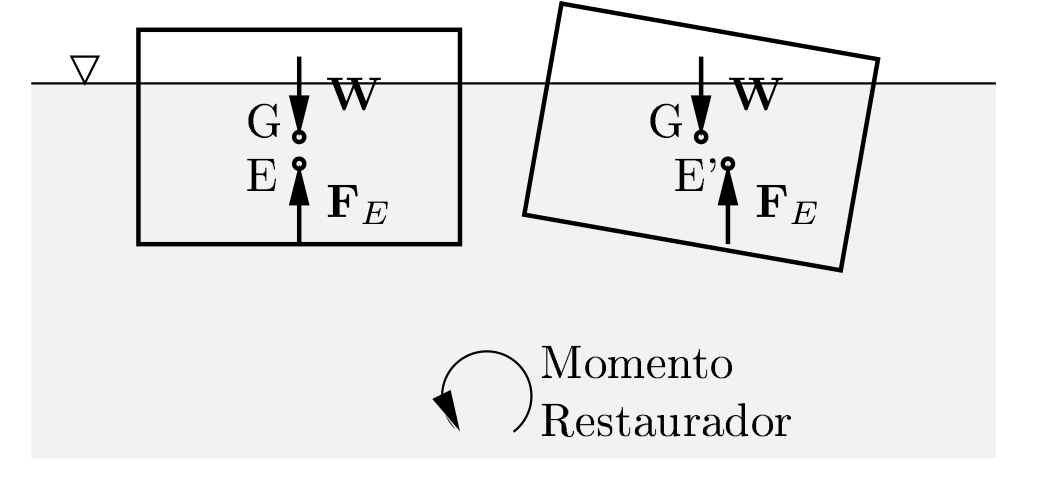
\includegraphics[width=0.7\linewidth]{TeX_files/chapter02-Hidrostatica/estabilidad2}
\end{center}



Equilibrio inestable
\begin{center}
	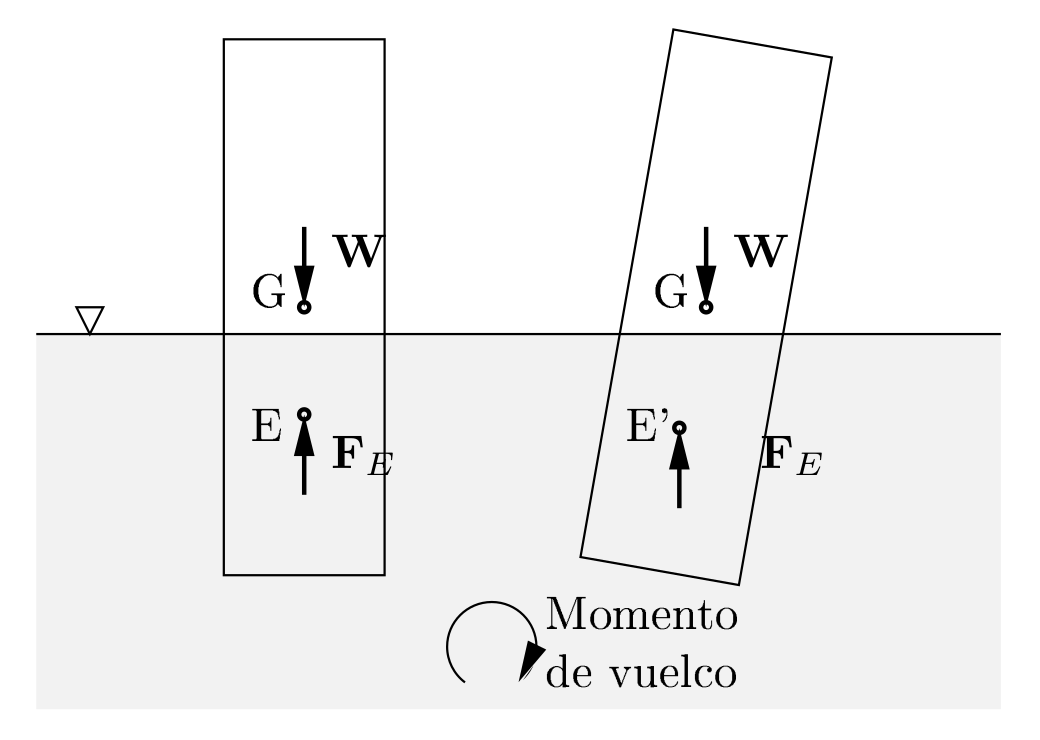
\includegraphics[width=0.7\linewidth]{TeX_files/chapter02-Hidrostatica/estabilidad3}
\end{center}


Pasos para calcular la estabilidad de un cuerpo flotante, consideremos un cuerpo sim\'etrico:

1.- Se calcula posici\'on de equilibrio inicial, mediante las fuerzas $\vec F_E$ y $\vec W$, y sus puntos de aplicaci\'on, $E$ y $G$. Como el cuerpo estan en equilibrio, estas fuerza se alinean con el eje de simetria.

2.- Se realiza una peque\~na perturbaci\'on $\Delta \theta$. El centro de empuje se desplaza a una nueva posici\'on $E'$. La vertical sobre $E'$ corta el eje de simetria en un punto $M$, denominado \textbf{metacentro}. Si el \'angulo $\Delta \theta$ es peque\~no, el metacentro no depender\'a de \'el.

3.- Se calcula la \textbf{altura metac\'entrica}, que es la distancia de $M$ a $G$. Si $M$ est\'a por encima de $G$, la altura metac\'entrica  es positiva, y la posici\'on es \emph{estable}. Si est\'a por debajo, la altura metac\'entrica es negativa, y la posici\'on es \emph{inestable}.

La altua metac\'entrica es una caracter\'istica de la secci\'on transversal del cuerpo y su distribuci\'on de masa.

\begin{center}
	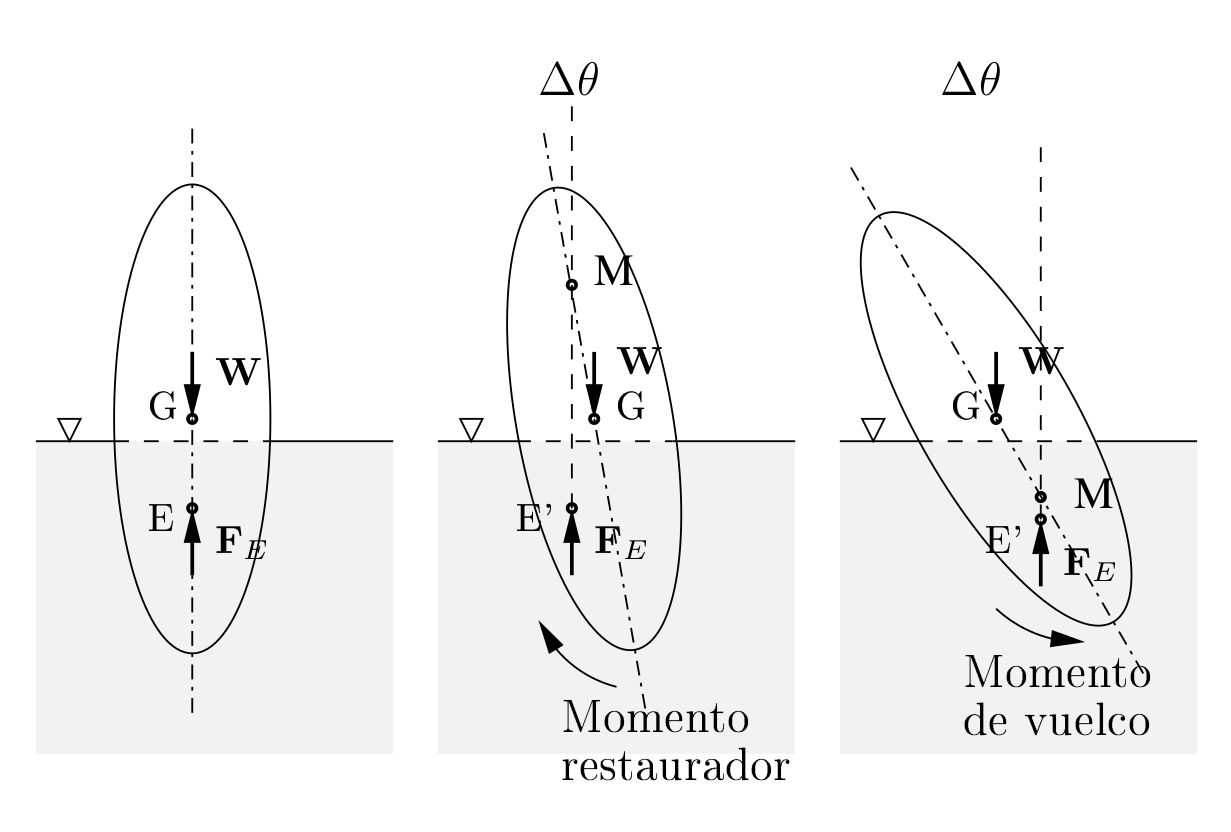
\includegraphics[width=0.7\linewidth]{TeX_files/chapter02-Hidrostatica/estabilidad4}
\end{center}

\begin{center}
	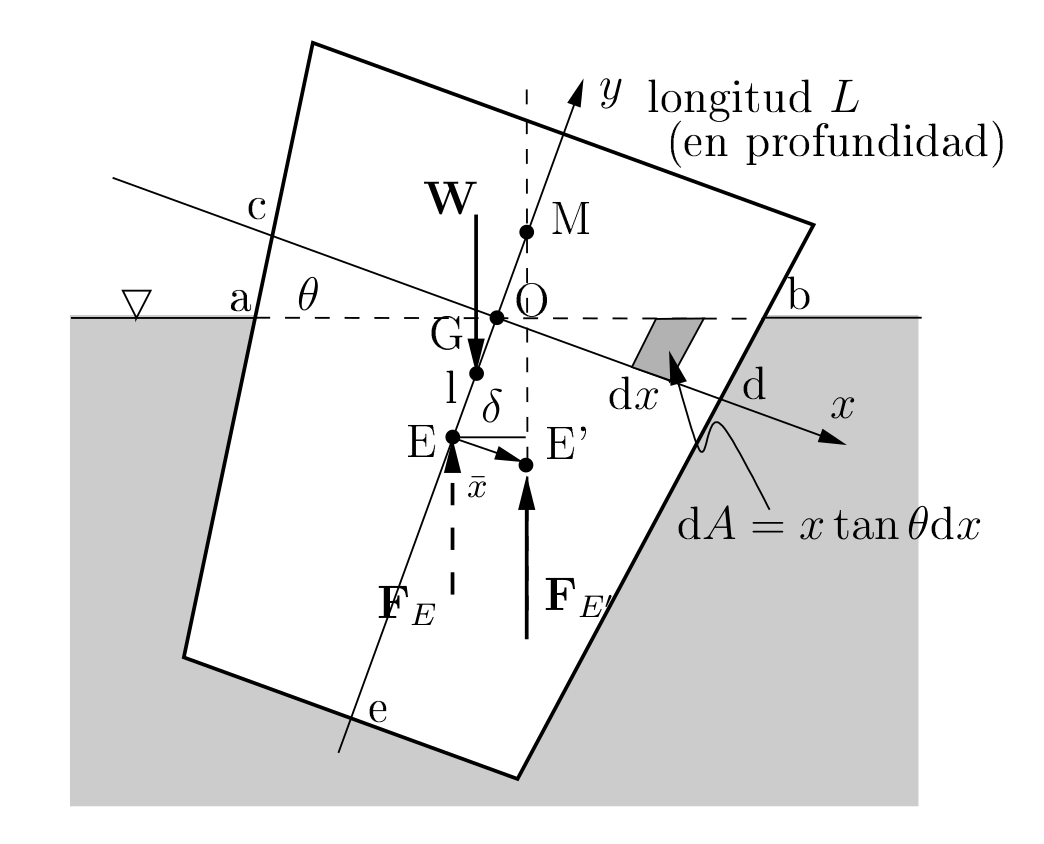
\includegraphics[width=0.7\linewidth]{TeX_files/chapter02-Hidrostatica/estabilidad5}
\end{center}




	La posici\'on del nuevo centro de empuje se calcula con la estimación del centro de masas:

\begin{align*}
	\overline{x}V_{aObdea} &= \int_{Obd}x \dif V - \int_{cOa} x \dif V
\\
	&= \int_{Obd} x L \dif A - \int_{cOa} x L \dif A 
\\
	&= \int_{Obd} x L (x\tan \theta \dif x) - \int_{cOa} x L  (-x\tan \theta \dif x)
\\
	&= \tan \theta \int x^2 2 L \dif x = \tan \theta \int x^2 \dif A 
	\\
	&= \tan \theta I_0
\end{align*}


La altura metac\'entrica es

\begin{equation}
	\overline{MG} = \overline{ME}-\overline{GE}= \frac{\overline{x}}{\tan \theta} - \overline{GE} 
= \frac{I_0}{V_{\textrm{sumergido}}} - \overline{GE} = \frac{\rho g I_0}{W} - \overline{GE}
\end{equation}

Si $\overline{MG}$ es positiva, el equilibrio es estable (para peque\~nas perturbaciones). Si 
$\overline{GE}$ es negativa, el equilibrio es estable siempre
\chapter{Cinemática de fluidos}
\section{Descripción Euleriana y Lagrangiana}
	
	Dos formas de identificación de las magnitudes (p. e., la velocidad) 
	\begin{enumerate}
		\item {\textbf{\textcolor{red}{Euleriana}}: \\
			Segun la \textcolor{blue}{posición} y el instante. 
		\begin{equation}
			\vec{u}(\vec{x},t)
		\end{equation}
		} 
		\item {\textbf{\textcolor{red}{Lagrangiana}}:\\
			Según la \textcolor{blue}{partí cula} y el instante. La partí cula
			queda identificada (marcada) mediante un vector $\vec{a}$ que puede
			ser, por ejemplo, la posición que tiene la partí cula en un instante
			de referencia $t_{0}$ 
			
\begin{equation}
				\vec{u}(\vec{a},t;t_{0})
\end{equation}
			
		} 
	\end{enumerate}


\section{Lineas de corriente, trayectorias y lineas de traza}

	
	\begin{itemize}
		\item \textcolor{red}{Lineas de corriente}:\\
		Para un instante dado $t_0$, és la tangente a los vectores de velocidad. 
	\end{itemize}

\begin{center}
	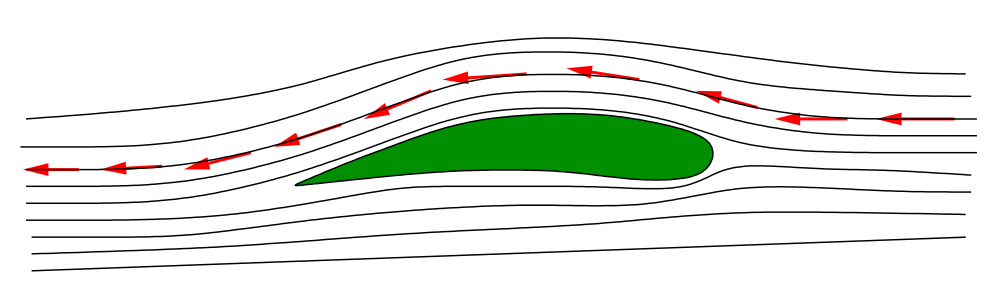
\includegraphics[width=0.7\linewidth]{TeX_files/chapter03-Cinematica/lineasCorriente}
\end{center}

		
		Són solución de la ecuación (en 2D) 
		
		\begin{equation}
			\frac{\text{d}x}{u(\vec{x},t=t_0)}=\frac{\text{d}y}{v(\vec{x},t=t_0)}
		\end{equation}
		


	
	\begin{itemize}
		\item \textcolor{red}{Trayectoria}:\\
		Para una cierta partícula de fluido, puntos que ocupa en un cierto
		intervalo de tiempo. 
		\item \textcolor{red}{Lineas de traza}:\\
		Partículas de fluido que, en un cierto instante anterior, pasaron
		por un determinado punto.
	\end{itemize}
\begin{center}
	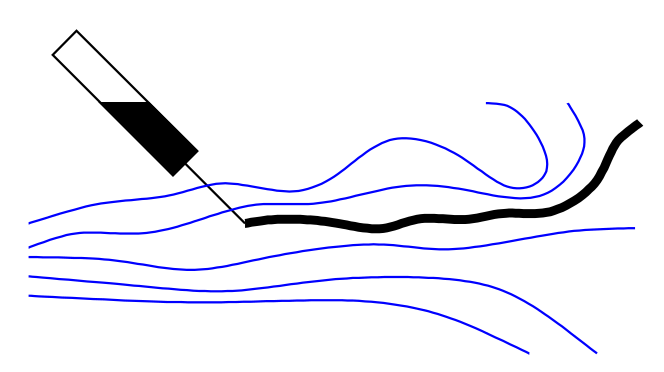
\includegraphics[width=0.5\linewidth]{TeX_files/chapter03-Cinematica/traza}
\end{center}


		
		Si el flujo es estacionario (no depende del tiempo), linea de corriente,
		trayectoria y linea de traza coinciden para un determinado punto. 
		



	
\subsection*{Actividad 1:}
		Dado el campo de velocidades bidimensional $\vec{u}=(x+t)\vec{\imath}+y\vec{\jmath}$,
		encontrad las expresiones para:
		
		a) la linea de corriente que pasa por $(1,1)$ para $t=0$
		
		b) la trayectoria de la partícula que está en $(1,1)$ para $t=0$
		
		c) la línea de traza, para $t=0$, de todas las partículas que pasaron
		por $(1,1)$


\section{Derivada sustancial}

	
	La partícula $P$, en el instante $t$ se encuentra en $\vec{x}$
	con una velocidad $\vec{u}$. La aceleración de $P$ \textbf{no} és
	$\dparc{\vec{u}}{t}$, ya que aunque $\vec{u}$ sea estacionario,
	$P$ puede estar moviéndose a un punto en que $\vec{u}$ és diferente.
	
	En un instante $t+\delta t$, $P$ estará en $\vec{x}+\delta\vec{x}=\vec{x}+\vec{u}\delta t$,
	de forma que la variación de velocidad será 
	\[
	\delta\vec{u}=\vec{u}(\vec{x}+\vec{u}\delta t,t+\delta t)-\vec{u}(\vec{x},t)
	\]
	
	Desarrollando en serie de Taylor hasta primer orden, obtenemos 
	\[
	\delta\vec{u}=\dparc{\vec{u}}{t}\delta t+(\vec{u}\cdot\vec{\nabla})\vec{u}\delta t+O(\delta t^{2}),
	\]
	de forma que la aceleración és 
	\[
	\vec{a}(\vec{x},t)=\dparc{\vec{u}}{t}+(\vec{u}\cdot\vec{\nabla})\vec{u}
	\]
	

De forma general, consideremos cualquier magnitud $f$, asociada a
una propiedad del fluido (puede ser un escalar como la temperatura,
o densidad, o la velocidad angular). 
\begin{itemize}
	\item Derivada \textcolor{red}{local}: 
	\[
	\dparc{f}{t}
	\]
	
	\item Derivada \textcolor{red}{convectiva}: 
	\[
	(\vec{u}\cdot\vec{\nabla})\vec{f}=\left(u\dparc{\phantom{f}}{x}+v\dparc{\phantom{f}}{y}+w\dparc{\phantom{f}}{z}\right)f=u_{i}\dparc{f}{x_{i}}
	\]
	
	\item Derivada \textcolor{red}{sustancial} o \textcolor{red}{total}: 
	\[
	\frac{\text{D}f}{\text{D}t}=\dparc{f}{t}+(\vec{u}\cdot\vec{\nabla})\vec{f}=\dparc{f}{t}+u_{i}\dparc{f}{x_{i}}
	\]
	
\end{itemize}

\section{Circulación, Flujo y Vorticidad}

	
	\begin{itemize}
		\item \textbf{\textcolor{red}{Circulación}}\\
		
		\[
		\Gamma=\oint_{L}\vec{u}\cdot\text{d}\vec{l}
		\]
		$L$ es cualquier contorno cerrado.
	\end{itemize}
	Si este contorno está constituido siempre por las mismas partí culas
	(es decir, es una línea material), se puede demostrar (\cite{Vir1})
	que 
	\[
	\Deriv{\Gamma}{t}=\Deriv{\phantom{t}}{t}\oint_{L}\vec{u}\cdot\text{d}\vec{l}=0
	\]
	

	
	\begin{itemize}
		\item \textbf{\textcolor{red}{Flujo}}\\
		Sea $F$ una magnitud extensiva propiedad del fluido y $f$ esta
		misma magnitud por unidad de volumen. El flujo de $f$ a través de
		la superficie $S$ es
	\end{itemize}
	\[
	\Phi=\int_{S}f\vec{u}\cdot\text{d}\vec{S}
	\]
	Si $f$ es un escalar, $f\vec{u}$ es el \textcolor{blue}{vector
		flujo} de $f$.
	
	Si $f$ es un vector $\left(\vec{f}\right)$ , $\vec{f}\vec{u}$ es
	el \textcolor{blue}{tensor flujo} de $f$.

	
{Ejemplo:}
		
		\[
		f=1\rightarrow\begin{cases}
			\vec{u} & \textrm{vector flujo volumétrico}\\
			Q=\int_{S}\vec{u}\cdot\text{d}\vec{S} & \textrm{flujo volumétrico, o caudal}
		\end{cases}
		\]
		
		\[
		f=\rho\rightarrow\begin{cases}
			\rho\vec{u} & \textrm{vector flujo másico}\\
			\dot{m}=\int_{S}\rho\vec{u}\cdot\text{d}\vec{S} & \textrm{flujo másico, o gasto}
		\end{cases}
		\]
		

\begin{itemize}
	\item \textbf{\textcolor{red}{Vorticidad}}\\
	
	\[
	\vec{\omega}=\vec{\nabla}\times\vec{u}\quad\text{En componentes:}\quad\omega_{k}=-\varepsilon_{ijk}\dparc{u_{i}}{x_{j}}
	\]
	Es el doble de la velocidad local de rotación del elemento de fluido.
	Por definición de vorticidad, se cumple que 
	\[
	\vec{\nabla}\cdot\vec{\omega}=0
	\]
	y el flujo a través de una superficie $S$ cerrada es siempre nulo
	\[
	\oint_{S}\vec{\omega}\cdot\text{d}\vec{S}=0
	\]
	\item Si la superficie es abierta, este flujo está relacionado con la circulación
	sobre la línea que limita la superficie a través del Teorema de Stokes
	\[
	\int_{S}\vec{\omega}\cdot\text{d}\vec{S}=\int_{S}\left(\vec{\nabla}\times\vec{u}\right)\cdot\text{d}\vec{S}=\oint_{L}\vec{u}\cdot\text{d}\vec{l}
	\]
	
\end{itemize}

\section{Movimiento relativo en el entorno de un punto}

	
	Sea $\vec{u}$ la velocidad del fluido en un punto $\vec{r}$. En
	un punto $\vec{r}+\delta\vec{r}$, la velocidad será $\vec{u}+\delta\vec{u}$,
	con 
	\[
	\delta\vec{u}=\vec{\nabla}\vec{u}\cdot\delta\vec{r};\ \delta u_{i}=\dparc{u_{i}}{x_{j}}\delta r_{j}
	\]
	
	El tensor \textcolor{blue}{divergencia de velocidad}, $\vec{\nabla}\vec{u}$,
	puede descomponerse como la suma de un tensor simétrico,$\left(\vec{\nabla}\vec{u}\right)^{S}$
	y un tensor antisimétrico $\left(\vec{\nabla}\vec{u}\right)^{A}$,
	con 
	\begin{eqnarray*}
		\left(\vec{\nabla}\vec{u}\right)^{S}=\frac{1}{2}\left(\vec{\nabla}\vec{u}+\left(\vec{\nabla}\vec{u}\right)^{T}\right)\\
		\left(\vec{\nabla}\vec{u}\right)^{A}=\frac{1}{2}\left(\vec{\nabla}\vec{u}-\left(\vec{\nabla}\vec{u}\right)^{T}\right)
	\end{eqnarray*}
	
	Cada uno de estos tensores contribuye a $\delta\vec{u}$ de una forma
	diferente 
	\[
	\delta\vec{u}=\delta\vec{u}^{S}+\delta\vec{u}^{A}=\left(\vec{\nabla}\vec{u}\right)^{S}\cdot\delta\vec{r}+\left(\vec{\nabla}\vec{u}\right)^{A}\cdot\delta\vec{r}
	\]
	

	
	$\delta\vec{u}^{S}=\left(\vec{\nabla}\vec{u}\right)^{S}\cdot\delta\vec{r}$
	representa un movimiento de \textcolor{blue}{deformación pura}. Siempre
	es posible escoger los ejes del sistema de referencia de forma que
	$\left(\vec{\nabla}\vec{u}\right)^{S}$ sea diagonal. Entonces los
	tres valores de la diagonal son las velocidades de estiramiento en
	la dirección de los ejes principales. Si el fluido es incompresible
	el volumen del elemento de fluido se mantiene constante y la suma
	de la diagonal, que es un invariante respecto del cambio de sistema
	de coordenadas, es nula 
	\[
	\dparc{u_{i}}{x_{i}}=0
	\]
	

	
	$\delta\vec{v}^{A}=\left(\vec{\nabla}\vec{u}\right)^{A}\cdot\delta\vec{r}$
	representa un movimiento de \textcolor{blue}{rotación pura}. 
	\[
	\delta u_{i}^{A}=\frac{1}{2}\left(\dparc{u_{i}}{x_{j}}-\dparc{u_{j}}{x_{i}}\right)\delta r_{j}=\frac{1}{2}\varepsilon_{ijk}\omega_{k}\delta r_{j}
	\]
	La velocidad angular de rotación es $\frac{1}{2}\vec{\omega}=\frac{1}{2}(\vec{\nabla}\times\vec{u})$. 


\chapter[Ecuaciones de la Dinámica]{Ecuaciones fundamentales de la Dinámica de los Fluidos}
\section{Introducción}
	
	La Mecánica de los fluidos viene determinada por \textcolor{red}{3
		leyes básicas}\footnote{Algunos autores, como \cite{Shames2003} toman en consideración también
		la Segunda Ley de la Termodinámica}
	
	\begin{itemize}
		\item \textcolor{black}{El principio de }\textcolor{red}{conservación de
			la masa}\textcolor{black}{. La masa de un sistema fluido se mantiene
			constante independientemente de su posición o forma. }
		\item \textcolor{black}{La ley de }\textcolor{red}{conservación de la cantidad
			de movimiento}\textcolor{black}{. La variación de la cantidad de movimiento
			de un sistema fluido es igual a la suma total de la fuerzas externas
			que actúan sobre él. }
		\item \textcolor{black}{La ley de }\textcolor{red}{conservación de la energía}\textcolor{black}{.
			Es, básicamente, la Primera Ley de la Termodinámica. La variación
			de la energía de un sistema fluido (energía interna + energía cinética)
			es igual al trabajo realizado por todos las fuerzas externas más el
			calor recibido por conducción y/o radiación. }
	\end{itemize}
	A estos principios hay que añadir las \textcolor{blue}{leyes constitutivas},
	como la ley de viscosidad de Newton, o la ley de los gases perfectos. 


\section{Formulación integral y diferencial}

	
	Existen dos enfoques para los problemas de Mecánica de Fluidos: 
	\begin{itemize}
		\item \textcolor{red}{Formulación diferencial}. Se consideran volumenes
		elementales de fluido y las ecuaciones que gobiernan su comportamiento.
		Para resolver los problemas con este planteamiento es necesario conocer
		las condiciones iniciales en todo el dominio y las condiciones de
		contorno en todos los límites del mismo. 
		\item \textcolor{red}{Formulación integral}. Se trabaja directamente sobre
		volumenes de fluido macroscópicos, denominados \textcolor{blue}{volúmenes
			de control}. Las ecuaciones son promediadas en el volumen de control
		y sobre su frontera, denominada \textcolor{blue}{superficie de control}. 
	\end{itemize}
	Para la mayoría de los problemas de Ingeniería ( o, por lo menos,
	para una primera aproximación) es suficiente con la formulación integral\footnote{La formulación diferencial es
		más general, y permite determinar detalles del flujo. Es posible extraer
		los resultados de la formulación integral a partir de los de la diferencial,
		pero no al contrario.}.


\subsection{Sistema y volumen de control}

	
	Un \textcolor{blue}{sistema de control} posee una cantidad definida
	de materia. Su volumen, y, por lo tanto, su densidad, así como otras
	magnitudes físicas pueden cambiar, pero no la cantidad de masa. En
	mecánica de sólidos se suele emplear el sistema de control como enfoque
	de trabajo.
	
	En Mecánica de Fluidos, es conveniente usar el enfoque de \textcolor{blue}{volúmen
		de control}, que se establece en el espacio, sin relación con una
	cierta cantidad de materia. Este volumen puede ser estático o no,
	y puede cambiar tanto de posición como de tamaño.
	
	La diferencia entre sistema y volumen de control se puede relacionar
	con la diferencia entre los puntos de vista Lagrangiano y Euleriano,
	ya que un sistema de control siempre sigue el movimiento de las partículas
	que lo componen.


\subsection{El teorema de arrastre de Reynolds}

	
	Dado que las ecuaciones de mecánica y termodinámica se refieren a
	sistemas de control, es necesario deducirlas para el caso en que las
	aplicamos sobre volúmenes de control.
	
	Consideremos un volumen de control y un sistema de control que, en
	un instante determinado $t$, coinciden en el espacio. El volumen
	de control $VC$ está estacionario, mientras que el sistema de control
	$V$ se mueve con el flujo.
	
		En el instante $t+\delta t$
				el sistema de control se encuentra en una posición ligeramente desplazada
				respecto al volumen. Incluso puede que haya cambiado su volumen, si
				el flujo es compresible
	
\begin{center}
	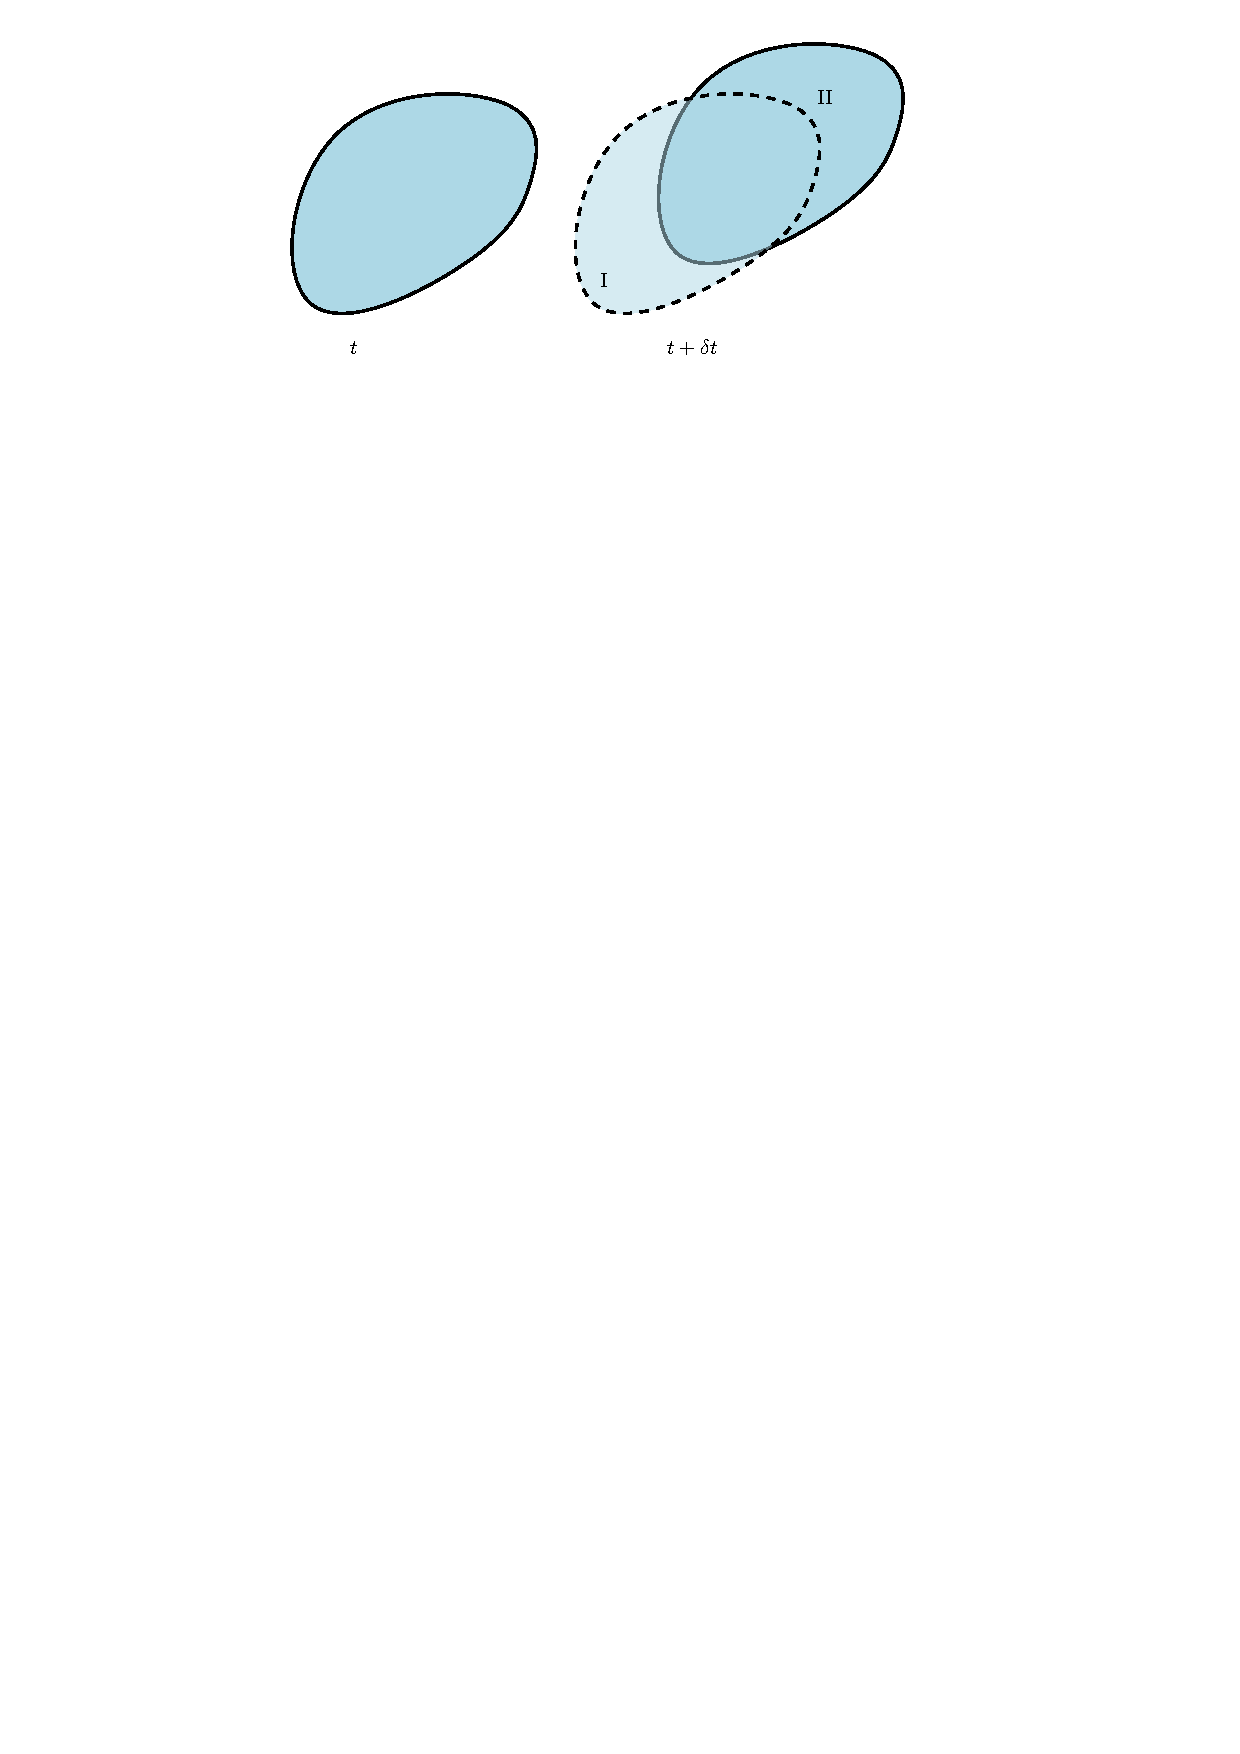
\includegraphics[width=0.7\linewidth]{TeX_files/chapter04-Dinamica/VC}
\end{center}


Consideremos una cierta magnitud extensiva $F$, y $f$ la misma por
unidad de masa, de forma que


\begin{equation}
	F=\int_{V}\rho f\,\text{d}V
\end{equation}


Consideremos la notación: \textcolor{black}{\scriptsize{}
	\begin{eqnarray*}
		F_{t} & : & \text{el valor de \ensuremath{F} para el sistema de control en el instante \ensuremath{t}}\\
		F_{t^{+}} & : & \text{el valor de \ensuremath{F} para el sistema de control en el instante \ensuremath{t+\delta t}}\\
		F'_{t} & : & \text{el valor de \ensuremath{F} para el volumen de control en el instante \ensuremath{t}}\\
		F'_{t^{+}} & : & \text{el valor de \ensuremath{F} para el volumen de control en el instante \ensuremath{t+\delta t}}\\
		F_{s} & : & \text{Cantidad de \ensuremath{F} que abandona el volumen de control en el intervalo \ensuremath{\Delta t} (a través de I)}\\
		F_{e} & : & \text{Cantidad de \ensuremath{F} que entra en el volumen de control en el intervalo \ensuremath{\Delta t} (a través de II)}
	\end{eqnarray*}
}{\scriptsize\par}

Evidentemente, 
\[
F_{t}=F'_{t}
\]


	
	Las variaciones de $F$ en el sistema de control y en el volumen de
	control son, respectivamente, 
	\begin{eqnarray*}
		\delta F & = & F_{t^{+}}-F_{t}\\
		\delta F' & = & F'_{t^{+}}-F'_{t}
	\end{eqnarray*}
	y, por otro lado, 
	\[
	F_{t^{+}}=F'_{t^{+}}+F_{s}-F_{e},
	\]
	de forma que 
	\[
	\delta F=\delta F'+F_{s}-F_{e}
	\]
	
	Dividiendo por $\delta t$ y haciendo el límite $\delta t\rightarrow0$,
	obtenemos 
	\[
	\deriv{F}{t}=\deriv{F'}{t}+\lim_{\delta t\rightarrow0}\frac{F_{s}-F_{e}}{\delta t}
	\]
	

	
	Por definición, el último término es el flujo de $F$ a través de
	la frontera de $VC$, que, como hemos definido en temas anteriores,
	
	\[
	\lim_{\delta t\rightarrow0}\frac{F_{s}-F_{e}}{\delta t}=\Phi_{F}=\oint_{SC}\rho f\vec{u}_{r}\cdot\text{d}\vec{S}
	\]
	
	\[
	\deriv{F}{t}=\deriv{F'}{t}+\oint_{SC}\rho f\vec{u}_{r}\cdot\text{d}\vec{S}
	\]
	

\begin{equation}
		\Rightarrow\boxed{\deriv{F}{t}=\deriv{\phantom{F}}{t}\int_{VC}\rho f\,\text{d}V+\oint_{SC}\rho f\vec{u}_{r}\cdot\text{d}\vec{S}}
\end{equation}
	,donde $\vec{u}_{r}$ es la velocidad del flujo relativa a la Superficie
	de Control.\\
	

	
	Otra forma de expresarlo es, usando el Teorema de Leibniz \cite[Sección 3.6]{Kundu2012}
	
\begin{equation}
		\boxed{\deriv{F}{t}=\int_{VC}\dparc{\rho f}{t}\,\text{d}V+\oint_{SC}\rho f\vec{u}\cdot\text{d}\vec{S}}
\end{equation}
	,donde $\vec{u}$ es ahora la velocidad absoluta. Si el VC no se mueve
	ni se deforma, $\vec{u}=\vec{u}_{r}$. 
	
	Se puede usar el Teorema de la Divergencia para transformar la integral
	de superficie en una integral de volumen, de forma que
	
	\[
	\deriv{F}{t}=\int_{VC}\dparc{\rho f}{t}\,\text{d}V+\int_{VC}\vec{\nabla}\cdot\left(\rho f\vec{u}\right)\text{d}V
	\]
	
	\[
	\Rightarrow\deriv{F}{t}=\int_{VC}\left[\dparc{\rho f}{t}+\vec{\nabla}\cdot\left(\rho f\vec{u}\right)\right]\text{d}V
	\]
	
\section{Ecuación integral de conservación de la masa}

	
	En este caso, $F=m$ y $f=1$. Por definición de sistema físico, $\deriv{m}{t}=0$,
	de forma que 
	\[
	\int_{VC}\dparc{\rho}{t}\,\text{d}V+\oint_{SC}\rho\vec{u}\cdot\text{d}\vec{S}=0
	\]
	
	\[
	\Rightarrow\,\boxed{\int_{VC}\dparc\rho t\,\dif V=-\oint_{SC}\rho\vec{u}\cdot\dif\vec{S}}
	\]
	
	Interpretación física: \textbf{\textcolor{red}{En un Volumen de Control,
			la variación local de la masa únicamente puede ser debida a un flujo
			de masa a través del contorno.}} 

	
	Simplicaciones de la ecuación integral de conservación de la masa
	\begin{itemize}
		\item Si el flujo es \textcolor{blue}{estacionario} en el interior del VC,
		entonces $\dparc{\rho}{t}=0$ y
		\[
		\oint_{SC}\rho\vec{u}\cdot\text{d}\vec{S}=0
		\]
		
		\item Si el flujo es \textcolor{blue}{incompresible}, entonces la densidad
		es constante en todo el VC, de forma que
		\[
		\int_{VC}\dparc\rho t\,\text{d}V=-\rho\oint_{SC}\vec{u}\cdot\text{d}\vec{S}
		\]
		
		\item Si se cumplen las dos condiciones y el flujo es \textcolor{blue}{incompresible
			y estacionario},
		\[
		\oint_{SC}\vec{u}\cdot\text{d}\vec{S}=0
		\]
	\end{itemize}


\subsection{Definición de velocidad media}

	
	Consideremos como caso simple un fluido incompresible circulando por
	una tubería. La sección de la tubería es $S$, y el flujo se puede
	considerar en todos los puntos axial, de forma que el caudal se calcula
	con 
	\[
	Q=\int_{S}u\text{d}S
	\]
	
	La \textcolor{red}{velocidad media} se define como la velocidad uniforme
	que debería tener el flujo para que el caudal fuese el mismo, $Q=\mean{u}S$.
	De aqui, 
	\[
	\mean{u}=\frac{1}{S}\int_{S}u\text{d}S
	\]
	\\
	Un documento muy interesante para estudiar la forma integral de la
	conservación de la masa, es el publicado en 2001 por el prof. Sonin,
	del MIT, disponible \href{http://web.mit.edu/2.25/www/pdf/cv.pdf}{aqui}.


\section{Ecuación diferencial de conservación de la masa}

	
	Aplicando el Teorema de la Divergencia a la forma integral, para un
	Volumen de Control estacionario, se obtiene 
	\[
	\int_{VC}\left[\dparc\rho t+\vec{\nabla}\cdot\left(\rho\vec{u}\right)\right]\text{d}V=0
	\]
	
	Como esto debe cumplirse para cualquier VC, obtenemos la forma diferencial
	de la conservación de la masa: 
	\[
	\dparc\rho t+\vec{\nabla}\cdot\left(\rho\vec{u}\right)=0
	\]
	
	En forma de componentes: 
	\[
	\dparc{\rho}{t}+\dparc{}{x_{i}}\left(\rho u_{i}\right)=0
	\]
	

\subsection{Líneas de corriente}

	
	Para un \textcolor{blue}{fluido incompresible}: 
	\[
	\vec{\nabla}\cdot\vec{u}=0
	\]
	
	\[
	\text{Flujo 2D}\quad\rightarrow\quad\dparc{u}{x}+\dparc{v}{y}=0
	\]
	
	Consideremos una función $\psi(x,y)$ que cumple 
	\[
	u=\dparc{\psi}{y}\quad;\quad v=-\dparc{\psi}{x}
	\]
	
	Entonces la ecuación de continuidad se cumple de forma exacta, ya
	que 
	\[
	\dparc{\phantom{x}}{x}\left(\dparc{\psi}{y}\right)+\dparc{\phantom{y}}{y}\left(-\dparc{\psi}{x}\right)\equiv0
	\]
	

	
	$\psi(x,y)$ es la \textcolor{red}{función de corriente}.
	
	Las líneas $\psi(x,y)=\psi_{i}=\text{cte}$ son las \textcolor{red}{líneas
		de corriente} y cumplen que 
	\[
	\text{d}\psi=0\Rightarrow\dparc{\psi}{x}\text{d}x+\dparc{\psi}{y}\text{d}y=0
	\]
	\[
	\Rightarrow-v\text{d}x+u\text{d}y=0\,\Rightarrow\,\frac{\text{d}x}{u}=\frac{\text{d}y}{v}
	\]
	
	es decir, son \emph{tangentes a $\vec{u}$} en todos los puntos

	
Interpretación física:
		
		Flujo bidimensional. Para una profundidad unidad:
		
\begin{center}
	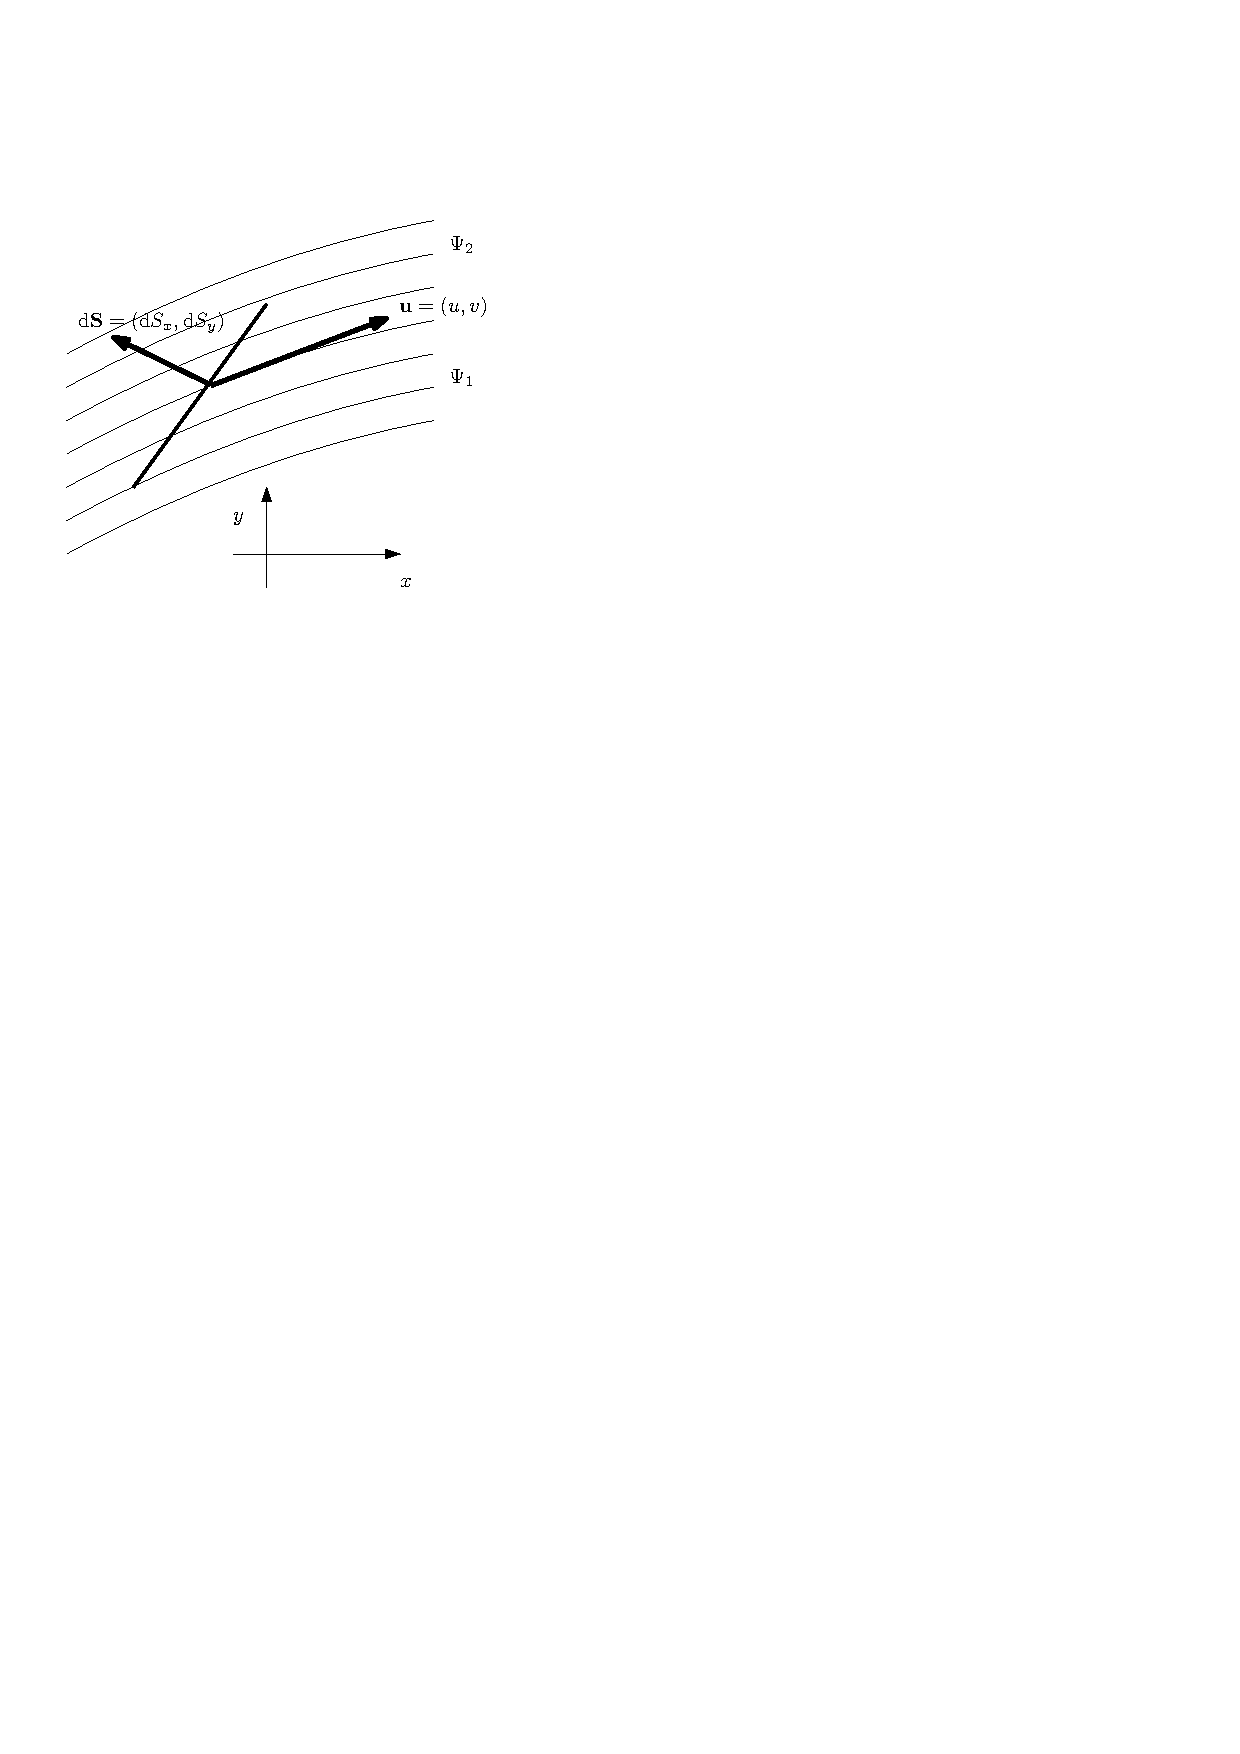
\includegraphics[width=0.4\linewidth]{TeX_files/chapter04-Dinamica/Phi1}
\end{center}

%			\input{interp_fisica_f_corr_2.pdftex_t}%
%		\end{minipage}\hfill{}%

			\begin{align*}
				dQ & =\vec{u}\cdot\text{d}\vec{S}\\
				 & =  \left(\begin{array}{cc}
					u & v\end{array}\right)\left(\begin{array}{c}
					\text{d}S_{x}\\
					\text{d}S_{y}
				\end{array}\right)\\
				& = \left(\begin{array}{cc}
					\dparc{\psi}{y} & -\dparc{\psi}{x}\end{array}\right)\left(\begin{array}{c}
					\text{d}y\\
					-\text{d}x
				\end{array}\right)(\times1)\\
				& =  \dparc{\psi}{y}\text{d}y+\dparc{\psi}{x}\text{d}x=\dif\psi\\
				\Rightarrow & \; Q=\psi_{2}-\psi_{1}
			\end{align*}


	
\subsection*{Actividad 1:}
		\[
		\vec{u}(x,y)=u(x,y)\,\vec{\imath}+v(x,y)\,\vec{\jmath}
		\]
		con $u(x,y)=a(x^{2}-y^{2})$. ?`Como tiene que ser de forma general
		$v(x,y)$ para que el flujo sea incompresible?
		
		Calcular la función de corriente y dibujar las lineas de corriente
		para el caso más simple.

\section{Ecuación integral de la conservación de la cantidad de movimiento}

	
	En este caso, $F=m\vec{u}$ y $f=\vec{u}$
	\textbf{Importante:}
		Carácter vectorial de $F$ y $f$
	
	T. de Transporte de Reynolds: 
	
	\begin{equation}
		\deriv{m\vec{u}}{t}=\deriv{\phantom{}}{t}\int_{VC}\rho\vec{u}\,\text{d}V+\oint_{SC}\rho\vec{u}\,\vec{u}_{r}\cdot\text{d}\vec{S}
	\end{equation}
	
	donde $\vec{u}_{r}$ es la velocidad relativa del fluido respecto
	de la $SC$, que no tiene por qué ser igual a $\vec{u}$, la velocidad
	relativa al Sistema de Referencia.

	
	Según la Segunda Ley de la Dinámica de Newton, 
	
\begin{equation}
		\deriv{m\vec{u}}{t}=\vec{F}_{T}
\end{equation}
	
	donde $\vec{F}$ es la suma total de \underline{todas} las fuerzas
	que actúan sobre el $VC$, tanto \textcolor{blue}{superficiales} como
	\textcolor{blue}{másicas}. Las fuerzas superficiales són producidas
	por todos los \textcolor{blue}{fluidos} y \textcolor{blue}{sólidos}
	incluidos en el $VC$.
	
	Debido al caracter vectorial de la cantidad de movimiento: 
	\begin{eqnarray}
		{F_{T}}_{x} & = & \deriv{\phantom{}}{t}\int_{VC}\rho u\,\text{d}V+\oint_{SC}\rho u\,\vec{u}_{r}\cdot\text{d}\vec{S}\\
		{F_{T}}_{y} & = & \deriv{\phantom{}}{t}\int_{VC}\rho v\,\text{d}V+\oint_{SC}\rho v\,\vec{u}_{r}\cdot\text{d}\vec{S}\\
		{F_{T}}_{z} & = & \deriv{\phantom{}}{t}\int_{VC}\rho w\,\text{d}V+\oint_{SC}\rho w\,\vec{u}_{r}\cdot\text{d}\vec{S}
	\end{eqnarray}
	


\section{Cálculo de fuerzas en un $VC$}

	
	Supongamos, por simplicidad, que el $VC$ está en reposo respecto
	del SR inercial.
	
	Las fuerzas superficiales que actúan sobre el material del VC són 
	\begin{itemize}
		\item tensiones de los sólidos que atraviesan el $VC$. 
		\item esfuerzos normales (presión) y tangenciales del fluido.\\
		Cálculo de presiones: 
		\[
		\vec{F}_{p}=-\oint_{SC}p\,\text{d}\vec{S}
		\]
		Si la presión és uniforme en toda la $SC$, $\vec{F}_{p}=0$. 
	\end{itemize}

	
	En muchas ocasiones los problemas prácticos de Ingeniería relacionados
	con la ecuación integral del conservación de la cantidad de movimiento
	són, básicamente, encontrar la fuerza que se ejerce sobre un cierto
	sólido en contacto con un fluido en movimiento.
	
	Ejemplos: 
	\begin{itemize}
		\item Fuerza sobre uniones en tuberías. 
		\item Fuerza sobre toberas, inyectores, \ldots{} 
		\item Fuerza sobre un vehículo aéreo o espacial. 
		\item Fuerza de un chorro sobre un obstáculo. 
		\item Fuerza sobre un vertedero. 
		\item \ldots{} 
	\end{itemize}
	La fuerza que se quiere calcular es siempre uno de los términos de
	$\vec{F}_{T}$. La raiz del problema estriba en aislar éste término
	en la relación de conservación de la cantidad de movimiento.

	
	\subsection*{Ejemplo (extraido de \cite{White2008}):}
		
\begin{center}
	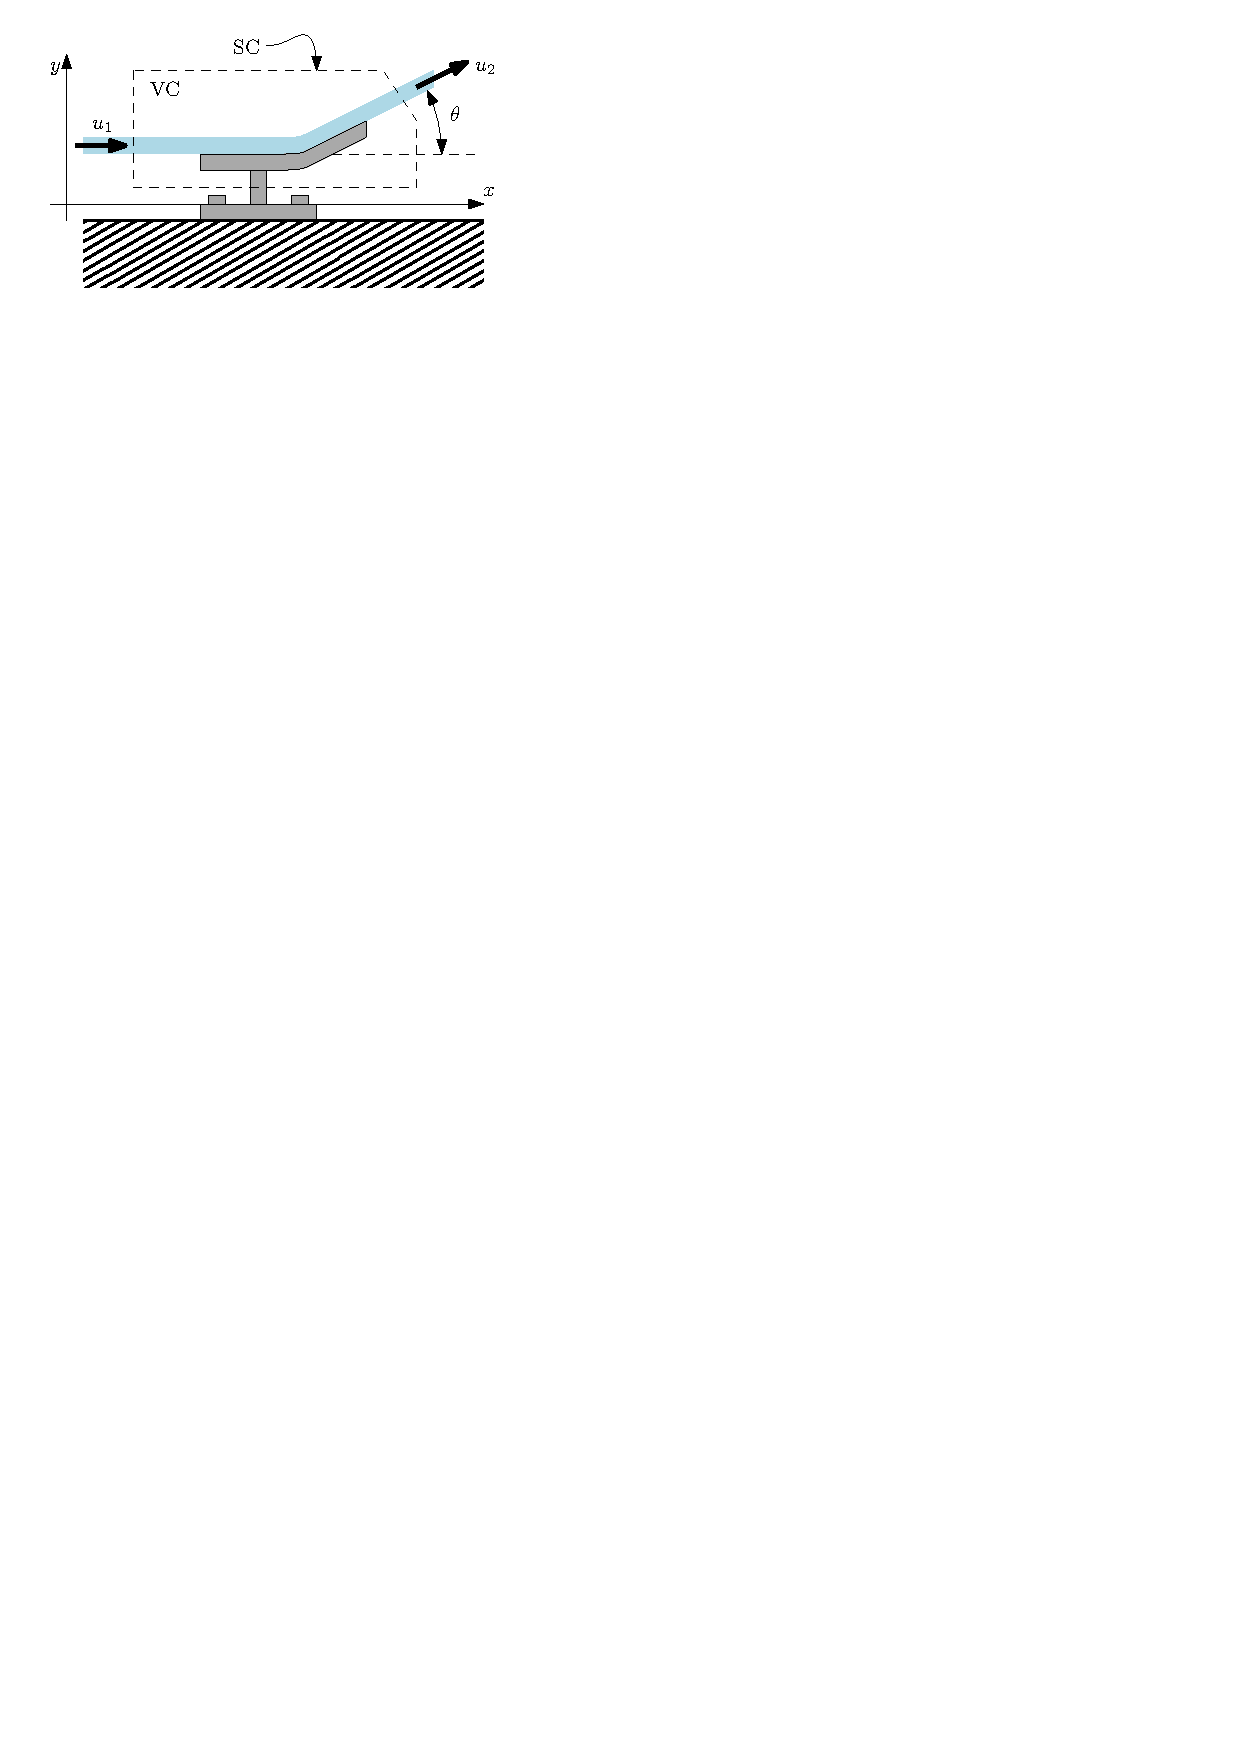
\includegraphics[width=0.5\linewidth]{TeX_files/chapter04-Dinamica/ejemploCM}
\end{center}

		
		Como hipótesis, suponemos que la sección del chorro es idéntica a
		la entrada y a la salida, de forma que, por la conservación de la
		masa, $\|\vec{u}_{1}\|=\|\vec{u}_{2}\|$.
		
		Queremos calcular la fuerza $\vec{F}$ que ejerce el chorro sobre
		el soporte.
		
		En realidad, lo que calcularemos será la fuerza $\vec{F}'$ que ejerce
		el soporte sobre el chorro. 
		
		Según la 3a. Ley de la Dinámica de Newton, $\vec{F}=-\vec{F}'$.

	

		\[
		\vec{F}'+\vec{F}_{m}+\vec{F}_{s}=\deriv{\phantom{}}{t}\int_{VC}\rho\vec{u}\,\text{d}V+\oint_{SC}\rho\vec{u}\,\vec{u}_{r}\cdot\text{d}\vec{S}
		\]
		$\vec{F}_{m}$: \emph{Fuerza de la gravedad.} Dado que no tenemos
		información sobre el volumen del chorro en el interior del VC, adoptamos
		la hipótesis de que $\|\vec{F}_{m}\|$ será muy pequeño en comparación
		con el resto de términos y, por lo tanto, lo despreciamos. A posteriori,
		debería comprobarse la validez de esta hipótesis.
		
		$\vec{F}_{s}$: \emph{Fuerza superficiales}, que engloban la presión
		y los esfuerzos tangenciales (fricción). Dado que la presión es uniforme,
		se anula. En cuanto a las fuerzas debidas a la fricción no hay ningun
		argumento para calcularlas, de forma que adoptamos la hipótesis de
		que són menospreciables.


		En cuanto al segundo miembro, el chorro es estacionario en el interior
		del VC, de forma que $\deriv{\phantom{}}{t}\int_{VC}\rho\vec{u}\,\text{d}V=0$
		
		La conservación de la cantidad de movimiento queda como 
		\[
		\vec{F}'=\oint_{SC}\rho\vec{u}\,\vec{u}\cdot\text{d}\vec{S}
		\]
		
		La velocidad sólo está definida en las secciones $S_{1}$ y $S_{2}$
		de $SC$, de forma que 
		\[
		\vec{F}'=\int_{S_{1}}\rho\vec{u}\,\vec{u}\cdot\text{d}\vec{S}+\int_{S_{2}}\rho\vec{u}\,\vec{u}\cdot\text{d}\vec{S}
		\]
		En componentes, según el SR de la figura, 
		\begin{eqnarray*}
			F'_{x} & = & \int_{S_{1}}\rho u\,\vec{u}\cdot\text{d}\vec{S}+\int_{S_{2}}\rho u\,\vec{u}\cdot\text{d}\vec{S}\\
			F'_{y} & = & \int_{S_{1}}\rho v\,\vec{u}\cdot\text{d}\vec{S}+\int_{S_{2}}\rho v\,\vec{u}\cdot\text{d}\vec{S}
		\end{eqnarray*}

	
		Es fácil ver que 
		\[
		\begin{array}{cc}
			\begin{cases}
				u=u & \text{en}\;S\\
				v=0 & \text{en}\;S_{1}
			\end{cases} & \begin{cases}
				u=u\cos\theta & \text{en}\;S_{2}\\
				v=u\sin\theta & \text{en}\;S_{2}
		\end{cases}\end{array}
		\]
		De forma que 
		\[
		\left\{ \begin{array}{ll}
			F'_{x} & =\int_{S_{1}}\rho u\vec{u}\cdot\text{d}\vec{S}+\int_{S_{2}}\rho u\cos\theta\vec{u}\cdot\text{d}\vec{S}\\
			& =\rho v\int_{S_{1}}\vec{u}\cdot\text{d}\vec{S}+\rho u\cos\theta\int_{S_{2}}\vec{u}\cdot\text{d}\vec{S}\\
			F'_{y} & =\int_{S_{2}}\rho u\sin\theta\vec{u}\cdot\text{d}\vec{S}=\rho u\sin\theta\int_{S_{2}}\vec{u}\cdot\text{d}\vec{S}
		\end{array}\right.
		\]
		
		\[
		\Rightarrow\left\{ \begin{array}{l}
			F'_{x}=\rho u(-Q)+\rho u\cos\theta Q=\rho uQ(cos\theta-1)\\
			F'_{y}=\rho u\sin\theta Q
		\end{array}\right.
		\]
		
		\[
		\Rightarrow\fbox{\ensuremath{\left\{  \begin{array}{l}
					F_{x}=\rho Su^{2}(1-\cos\theta)\\
					F_{y}=-\rho Su^{2}\sin\theta
				\end{array}\right.}}
		\]

	
	\subsection*{Actividad 1:}
		Una manguera antiincendios, de 10 cm de diámetro, da 100 l/s de
		agua con una presión de 1600 kPa. Al final de la manguera hay un inyector
		que reduce el diámetro a 2,5 cm. Estima suponiendo que ésta és la
		presión al llegar el agua al inyector, la fuerza que ejerce el agua
		sobre el mismo.


\subsection{Sistema de Referencia No Inercial}
	
	El SR está ahora acelerado. La conservación de la cantidad de movimiento
	es 
	\[
	\vec{F}_{T}-\int_{VC}\rho\vec{a}'\text{d}V=\int_{VC}\dparc{\rho\vec{u}}{t}\,\text{d}V+\oint_{SC}\rho\vec{u}\,\vec{u}\cdot\text{d}\vec{S}
	\]
	donde 
	\[
	\vec{a}'=\underbrace{\frac{\text{d}^{2}\vec{R}}{\text{d}t^{2}}}_{\text{ac. lineal del SR}}+\underbrace{\deriv{\vec{\Omega}}{t}\times\vec{r}}_{\text{ac. angular del SR}}+\underbrace{2\left(\vec{\Omega}\times\vec{u}\right)}_{\text{ac. de Coriolis}}+\underbrace{\vec{\Omega}\times\left(\vec{\Omega}\times\vec{r}\right)}_{\text{ac. centr\'\i fuga}}
	\]
	


\subsection{Factor de corrección de flujo de cantidad de movimiento}

	
	Flujo de cantidad de movimiento: 
	\[
	\Phi=\int_{S}\rho\vec{u}\left(\vec{u}\cdot\text{d}\vec{S}\right)
	\]
	
	Supongamos que $\vec{u}\parallel\text{d}\vec{S}$ y $\vec{u}=u\vec{\imath}$
	en todo $S$ (p. e., en una tubería), de forma que $\Phi=\int_{S}\rho u^{2}\text{d}S$
	
	A veces es conveniente relacionarlo con la velocidad media, $\Phi=\beta\rho\overline{u}^{2}S$,
	donde $\beta>1$ es un factor de conversión, que se calcula mediante
	\[
	\beta=\frac{1}{S}\int\left(\frac{u}{\overline{u}}\right)^{2}\text{d}S
	\]
	si el fluido es incompresible.
	\subsection*{Actividad 2:}
		
		Calcular el valor de $\beta$ para un perfil parabólico de velocidad. 

\section{Ecuación diferencial de la conservación de la cantidad de movimiento}

	
	La ecuación integral es, aplicando el TRR: 
	
	\begin{equation}
		\int_{VC}\dparc{\phantom{t}}{t}\left(\rho\vec{u}\right)\text{d}V+\oint_{SC}\rho\vec{u}\left(\vec{u}\cdot\text{d}\vec{S}\right)=\vec{F}_{T}
	\end{equation}
	
	
	Aplicando el Teorema de la Divergencia a la integral sobre la Superficie
	de Control (ver, p.e., \cite{Liggett1994}, pag. 6), 
	
	\begin{equation}
		\oint_{SC}\rho\vec{u}\left(\vec{u}\cdot\text{d}\vec{S}\right)=\int_{VC}\vec{\nabla}\cdot\left(\vec{u}\rho\vec{u}\right)\text{d}V
	\end{equation}
	
	obtenemos 
	
	\begin{equation}
		\int_{VC}\left[\dparc{\phantom{t}}{t}\left(\rho\vec{u}\right)+\vec{\nabla}\cdot\left(\vec{u}\rho\vec{u}\right)\right]\text{d}V=\vec{F}_{T}
	\end{equation}
	
	
	
	Por tanto, la fuerza sobre un volumen elemental de fluido es 
	\begin{eqnarray}
		\vec{f}_{T} & = & \dparc{\phantom{t}}{t}\left(\rho\vec{u}\right)+\vec{\nabla}\cdot\left(\vec{u}\rho\vec{u}\right)\\
		& = & \dparc{\phantom{t}}{t}\left(\rho\vec{u}\right)+\dparc{\phantom{x}}{x}\left(\rho u\vec{u}\right)+\dparc{\phantom{y}}{y}\left(\rho v\vec{u}\right)+\dparc{\phantom{z}}{z}\left(\rho w\vec{u}\right)
	\end{eqnarray}
	
	En forma de componentes: 
	\begin{eqnarray}
		{f_{T}}_{x} & = & \dparc{\phantom{t}}{t}\left(\rho u\right)+\dparc{\phantom{x}}{x}\left(\rho u^{2}\right)+\dparc{\phantom{y}}{y}\left(\rho vu\right)+\dparc{\phantom{z}}{z}\left(\rho wu\right)\\
		{f_{T}}_{y} & = & \dparc{\phantom{t}}{t}\left(\rho v\right)+\dparc{\phantom{x}}{x}\left(\rho uv\right)+\dparc{\phantom{y}}{y}\left(\rho v^{2}\right)+\dparc{\phantom{z}}{z}\left(\rho wv\right)\\
		{f_{T}}_{z} & = & \dparc{\phantom{t}}{t}\left(\rho w\right)+\dparc{\phantom{x}}{x}\left(\rho uw\right)+\dparc{\phantom{y}}{y}\left(\rho vw\right)+\dparc{\phantom{z}}{z}\left(\rho w^{2}\right)
	\end{eqnarray}
	

	
	Podemos simplificar un poco usando 
	\begin{eqnarray}
		\dparc{\phantom{t}}{t}\left(\rho\vec{u}\right) & = & \vec{u}\,\dparc{\rho}{t}+\rho\,\dparc{\vec{u}}{t}\\
		\dparc{\phantom{x}}{x}\left(\rho u\vec{u}\right) & = & \vec{u}\,\dparc{\rho u}{x}+\rho u\,\dparc{\vec{u}}{x}\\
		\dparc{\phantom{y}}{y}\left(\rho v\vec{u}\right) & = & \vec{u}\,\dparc{\rho v}{y}+\rho v\,\dparc{\vec{u}}{y}\\
		\dparc{\phantom{z}}{z}\left(\rho w\vec{u}\right) & = & \vec{u}\,\dparc{\rho w}{x}+\rho w\,\dparc{\vec{u}}{z}
	\end{eqnarray}
	
	\begin{eqnarray}
		\Rightarrow\vec{f}_{T} & = & \vec{u}\,\dparc{\rho}{t}+\rho\,\dparc{\vec{u}}{t}+\vec{u}\left(\vec{\nabla}\cdot\rho\vec{u}\right)+\rho\left(\vec{u}\cdot\nabla\right)\vec{u}\\
		& = & \vec{u}\cdot\underbrace{\left[\dparc{\rho}{t}+\vec{\nabla}\cdot\rho\vec{u}\right]}_{=0\;\text{por continuidad}}+\rho\,\dparc{\vec{u}}{t}+\rho\left(\vec{u}\cdot\vec{\nabla}\right)\vec{u}
	\end{eqnarray}
	

	
	La \textcolor{red}{ecuación diferencial de conservación de la cantidad
		de movimiento} queda como 
	
	\begin{equation}
		\boxed{\vec{f}_{T}=\rho\,\dparc{\vec{u}}{t}+\rho\left(\vec{u}\cdot\vec{\nabla}\right)\vec{u}}
	\end{equation}
	
	
	Para simplificar, supongamos que 
	\[
	\vec{f}_{T}=\text{gravedad}+\text{fricción fluido-fluido}
	\]
	
	\[
	\vec{f}_{T}=\rho\vec{g}+\vec{\nabla}\cdot\vec{\vec{\tau}}
	\]
	de forma que 
	
	\begin{equation}
		\rho\,\dparc{\vec{u}}{t}+\rho\left(\vec{u}\cdot\vec{\nabla}\right)\vec{u}=\rho\vec{g}+\vec{\nabla}\cdot\vec{\vec{\tau}}
	\end{equation}
	
	
	En forma de componentes: 
	
	\begin{equation}
		\rho\left(\dparc{u_{i}}{t}+u_{j}\dparc{u_{i}}{x_{j}}\right)=\rho g_{i}+\dparc{\tau_{ij}}{x_{j}}
	\end{equation}
	
	

\section{El tensor de tensiones para fluidos newtonianos. La ecuación de Navier-Stokes}

	
	El mayor problema de la ecuación anterior es el cálculo de $\vec{\vec{\tau}}$.
	Éste tensor agrupa tanto los esfuerzos normales como los tangenciales.
	
	Los esfuerzos normales no són la presión, ya que ésta no está definida
	de forma estricta para fluidos en movimiento(ver \cite{Batchelor1997},
	capítulo 3), pero se puede definir una presión análoga a la usada
	en fluidostática de la forma $p=-\frac{1}{3}\tau_{ii}$
	
	De esta forma, el tensor de tensiones es 
	\[
	\tens=\underbrace{-p\mathbb{I}}_{\text{parte isótropa}}+\underbrace{\tens'}_{\begin{footnotesize}\begin{array}{c}
				\text{parte anisótropa (con traza nula)}\end{array}\end{footnotesize}}
	\]
	
	\[
	=\left(\begin{array}{ccc}
		-p & 0 & 0\\
		0 & -p & 0\\
		0 & 0 & -p
	\end{array}\right)+\left(\begin{array}{ccc}
		\tau_{xx}+p & \tau_{xy} & \tau_{xz}\\
		\tau_{yx} & \tau_{yy}+p & \tau_{yz}\\
		\tau_{zx} & \tau_{zy} & \tau_{zz}+p
	\end{array}\right)
	\]
	
	
	Se puede demostrar(ver, p.e., \cite{Batchelor1997} o \cite{CrespoMartinez2006})
	que, para \textcolor{blue}{fluidos newtonianos}, $\tens'$ está relacionado
	con la parte simétrica de la divergencia de la velocidad (ver el segundo
	tema de cinemática) mediante 
	
\begin{equation}
		\tens'=2\mu\left[\left(\vec{\nabla}\vec{u}\right)^{S}-\frac{1}{3}\left(\vec{\nabla}\cdot\vec{u}\right)\mathbb{I}\right]
\end{equation}
	
	donde $\mu$ es la viscosidad dinámica.
	
	Substituyendo en la ecuación diferencial de la conservación de la
	cantidad de movimiento, 
	
	\begin{equation}
		\rho\,\dparc{\vec{u}}{t}+\rho\left(\vec{u}\cdot\vec{\nabla}\right)\vec{u}=\rho\vec{g}-\vec{\nabla}p+\vec{\nabla}\cdot\left\{ 2\mu\left[\left(\vec{\nabla}\vec{u}\right)^{S}-\frac{1}{3}\left(\vec{\nabla}\cdot\vec{u}\right)\mathbb{I}\right]\right\}
	\end{equation}
	
	,que es la \textcolor{red}{ecuación de Navier-Stokes}.

	
	En la mayoría de los casos, se puede considerar que \textcolor{blue}{$\mu$
		es uniforme}, de forma que, tras algunas operaciones tensoriales,
	
	\begin{equation}
		\rho\,\dparc{\vec{u}}{t}+\rho\left(\vec{u}\cdot\vec{\nabla}\right)\vec{u}=\rho\vec{g}-\vec{\nabla}p+\mu\left[\triangle\vec{u}+\frac{1}{3}\vec{\nabla}\left(\vec{\nabla}\cdot\vec{u}\right)\right]
	\end{equation}
	
	con 
	
	\begin{equation}
		\laplace\equiv{\vec{\nabla}}^{2}=\dparcsec{\phantom{x}}{x}+\dparcsec{\phantom{y}}{y}+\dparcsec{\phantom{z}}{z}
	\end{equation}
	
	
	Si el \textcolor{blue}{flujo es incompresible}, $\vec{\nabla}\cdot\vec{u}=0$,
	y la ecuación de Navier-Stokes queda como 
	
\begin{equation}
		\boxed{\rho\,\dparc{\vec{u}}{t}+\rho\left(\vec{u}\cdot\vec{\nabla}\right)\vec{u}=\rho\vec{g}-\vec{\nabla}p+\mu\triangle\vec{u}}
\end{equation}
	
	
	En forma de componentes, 
	
	\begin{equation}
		\rho\left(\dparc{u_{i}}{t}+u_{j}\dparc{u_{i}}{x_{j}}\right)=\rho g_{i}-\dparc{p}{x_{i}}+\mu\frac{\partial^{2}u_{i}}{\partial x_{j}\partial x_{j}}
	\end{equation}
	

	

		Si menospreciamos los efectos de la viscosidad (flujo inviscido),
		tenemos la \textcolor{red}{Ecuación de Euler} 
		\[
		\rho\,\dparc{\vec{u}}{t}+\rho\left(\vec{u}\cdot\vec{\nabla}\right)\vec{u}=\rho\vec{g}-\vec{\nabla}p
		\]

	\subsection*{Actividad 1:}
		Escribid las ecuaciones de la dinámica de un flujo laminar entre
		dos placas paralelas, sin presión pero con viscosidad. La velocidad
		tan sólo tiene componente $x$, y las placas son normales a la dirección
		$y$. El flujo es estacionario. 
		
		¿Como cambian las ecuaciones si no hay viscosidad (Ecuación de Euler)?
		
\section{Ecuación integral de la conservación del momento cinético}

	
	Es posible aplicar la forma general de conservación de una magnitud
	física al momento cinético.
	
	Recordemos que para una partícula, su momento cinético respecto de
	un punto $O$ se define como 
	\[
	\vec{L}_{0}=\vec{r}_{0}\times m\vec{u}
	\]
	y la física de partículas dice que la derivada de esta magnitud es
	igual a la suma de los momentos de las fuerzas que actúan sobre la
	partícula 
	\[
	\deriv{\vec{L}_{0}}{t}=\sum\left(\vec{r}_{0}\times\vec{F}\right)={\vec{M}_{T}}
	\]
	

	
	Apliquemos esto a un Volumen de Control relacionado con un fluido.
	Para un Sistema de Control, el momento cinético es 
	
	\begin{equation}
		\vec{L}_{0}=\int_{\text{Sist C}}\left(\vec{r}_{0}\times\vec{u}\right)\rho\dif V
	\end{equation}
	
	y, aplicando el teorema de transporte de Reynolds, con 
	\[
	F=\vec{r}_{0}\times m\vec{u}
	\]
	y 
	\[
	f=\vec{r}_{0}\times\vec{u},
	\]
	la variación de esta magnitud para un Volumen de Control, es 
	
	\begin{equation}
		{\vec{M}_{T}}=\deriv{\vec{L}_{0}}{t}=\int_{VC}\dparc{\left(\vec{r}_{0}\times\rho\vec{u}\right)}{t}\dif V+\oint_{SC}\left(\vec{r}_{0}\times\vec{u}\right)\rho\vec{u}\cdot\dif\vec{S}
	\end{equation}
	
	
	
	Es importante no olvidar, igual que en la conservación de la cantidad
	de movimiento, el caracter vectorial de esta relación.
	
	Omitiendo el subíndice $0$, en componentes esta relación es 
	\begin{eqnarray}
		{M_{T}}_{x} & = & \int_{VC}\dparc{\rho\left(yw-zv\right)}{t}\dif V+\oint_{SC}\rho\left(yw-zv\right)\,\vec{u}\cdot\dif\vec{S}\\
		{M_{T}}_{y} & = & \int_{VC}\dparc{\rho\left(zu-xw\right)}{t}\dif V+\oint_{SC}\rho\left(zu-xw\right)\,\vec{u}\cdot\dif\vec{S}\\
		{M_{T}}_{x} & = & \int_{VC}\dparc{\rho\left(xv-yu\right)}{t}\dif V+\oint_{SC}\rho\left(xv-yu\right)\,\vec{u}\cdot\dif\vec{S}
	\end{eqnarray}
	
	El momento total $\vec{M}_{T}$ es el producido por todas las fuerzas
	externas, másicas y superficiales.


\section{Cálculo de momentos en un VC}

	
	\begin{itemize}
		\item \textbf{Sistema de referencia inercial}
	\end{itemize}
	Supongamos como caso más simple un Volumen de Control no deformable
	y inercial, tal que todas las propiedades del fluido (densidad, velocidad,
	posición,\ldots ) pueden ser consideradas uniformes en las secciones
	de entrada y salida (es decir, el flujo puede ser considerado unidimensional). 
	
	En este caso, la conservación del momento cinético se expresa como
	
\begin{equation}
		\vec{M}_{T}=\int_{VC}\dparc{\left(\vec{r}_{0}\times\rho\vec{u}\right)}{t}\dif V+\sum_{salidas}\left(\vec{r}\times\vec{u}\right)\dot{m}_{sal}-\sum_{entradas}\left(\vec{r}\times\vec{u}\right)\dot{m}_{ent}
\end{equation}
	
	

	
	\subsection{Ejemplo 1:}
		
		\begin{center}
			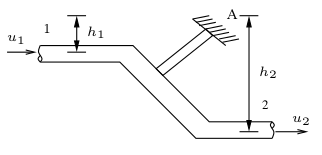
\includegraphics[width=0.5\linewidth]{TeX_files/chapter04-Dinamica/ejemplo1CMC}
		\end{center}
		
		
		Queremos calcular el momento sobre el punto A, usando el Volumen de
		Control mostrado en la siguiente figura.
		
		\begin{center}
			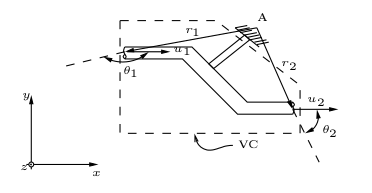
\includegraphics[width=0.5\linewidth]{TeX_files/chapter04-Dinamica/ejemplo1CMC1}
		\end{center}
		

		Suponemos que las propiedades del fluido (velocidad, densidad, presión)
		son uniformes en la entrada y en la salida, que el flujo es estacionario
		y que el peso del fluido y la tubería son menospreciables, asi como
		los efectos del rozamiento. Con estas hipótesis, la conservación del
		momento cinético es 
		\[
		\vec{M}_{T}=\vec{M}_{A}+\left[\vec{r}_{1}\times\left(-p_{1}\vec{S}_{1}\right)\right]+\left[\vec{r}_{2}\times\left(-p_{2}\vec{S}_{2}\right)\right]
		\]
		
		\[
		=\left(\vec{r}_{2}\times\vec{u}_{2}\right)\dot{m}_{2}-\left(\vec{r}_{1}\times\vec{u}_{1}\right)\dot{m}_{1}
		\]
		$\vec{M}_{A}$ es el momento realizado por la tubería \textbf{sobre}
		el fluido y transmitido a través del brazo al empotramiento en A.
		
		Dado que el flujo es unidimensional y los vectores de posición solo
		tienen componentes en $x$ y en $y$, los momentos son en la dirección
		$z$.

		Los módulos de los momentos que hacen las presiones son 
		\[
		\begin{cases}
			\left|\vec{r}_{1}\times\left(-p_{1}\vec{S}_{1}\right)\right| & =r_{1}p_{1}S_{1}\sin\theta_{1}=p_{1}S_{1}h_{1}\\
			\left|\vec{r}_{2}\times\left(-p_{2}\vec{S}_{2}\right)\right| & =-r_{2}p_{2}S_{2}\sin\theta_{2}=-p_{2}S_{2}h_{2}
		\end{cases}
		\]
		
		La variación de momento cinético del fluido es 
		\begin{align*}
			\left(\vec{r}_{2}\times\vec{u}_{2}\right)\dot{m}_{2}-\left(\vec{r}_{1}\times\vec{u}_{1}\right)\dot{m}_{1}=\left(r_{2}u_{2}\sin\theta_{2}-r_{1}u_{1}\sin\theta_{1}\right)\dot{m}\\
			\dot{m}=\left(h_{2}u_{2}-h_{1}u_{1}\right)
		\end{align*}
		
		Combinando todo, obtenemos $M_{A}$, 
		\[
		M_{A}=\left(h_{2}u_{2}-h_{1}u_{1}\right)\dot{m}-p_{1}S_{1}h_{1}+p_{2}S_{2}h_{2}
		\]
		\[
		=h_{2}\left(u_{2}\dot{m}+p_{2}S_{2}\right)-h_{1}\left(u_{1}\dot{m}+p_{1}S_{1}\right)
		\]
	
	\subsection*{Ejemplo 2:}
		Un irrigador por aspersion de radio $R$ da vueltas con una velocidad
		angular $\vec{\omega}=\omega\vec{k}$ y expulsa un caudal $Q$ por
		una tubería de sección $S$. El rozamiento sobre el eje es $\vec{M}_{r}=-M_{r}\vec{k}$.
		Queremos encontrar en el equilibrio una expresión para $\omega$.
		
		\begin{center}
			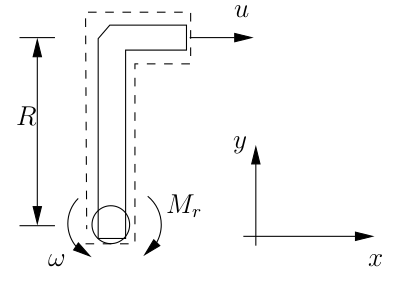
\includegraphics[width=0.5\linewidth]{TeX_files/chapter04-Dinamica/ejemplo2CMC}
		\end{center}
		
	

		Suponemos que el flujo es estacionario e incompresible, y que el peso
		del fluido y del irrigador son menospreciables. Despreciamos tambien
		los efectos de la fricción en el fluido. El brazo del irrigador no
		es estacionario, pero \textbf{sí} lo es el VC, de forma que la velocidad
		$u_{2}$ que pasa a través de la SC en la salida no es $u=\frac{Q}{S}$,
		sino 
		\[
		u_{2}=u-\omega R
		\]
		
		En el equilibrio, se cumple que 
		\[
		\vec{M}_{T}=-M_{r}\vec{k}=\left(\vec{r}_{2}\times\vec{u}_{2}\right)\dot{m}_{2}-\left(\vec{r}_{1}\times\vec{u}_{1}\right)\dot{m}_{1}
		\]
		Dado que $r_{1}=0$, tenemos $-M_{r}\vec{k}=\left(R\vec{\jmath}\times u_{2}\vec{\imath}\right)\dot{m}=-Ru_{2}\dot{m}\vec{k}$
		\begin{align*}
			M_{r}=\rho QR\left(u-\omega R\right)\\
			\omega=\frac{u}{R}-\frac{M_{r}}{\rho QR^{2}}=\frac{Q}{RS}-\frac{M_{r}}{\rho QR^{2}}
		\end{align*}

	
	\begin{itemize}
		\item \textbf{Sistema de referencia no inercial}
	\end{itemize}
	La única diferencia es que hay que añadir a los momentos realizados
	por las fuerzas externas, los momentos de las aceleraciones ficticias,
	
	\[
	\vec{M}_{T}-\int_{VC}\rho\left(\vec{r}_{0}\times\vec{a}'\right)\dif V=\int_{VC}\dparc{\left(\vec{r}_{0}\times\rho\vec{u}\right)}{t}\dif V+\oint_{SC}\left(\vec{r}_{0}\times\vec{u}\right)\rho\vec{u}\cdot\dif\vec{S}
	\]
	donde, tal y como vimos en el tema de conservación de la cantidad
	de movimiento, 
	\[
	\vec{a}'=\underbrace{\frac{\text{d}^{2}\vec{R}}{\text{d}t^{2}}}_{\text{ac. lineal del SR}}+\underbrace{\deriv{\vec{\Omega}}{t}\times\vec{r}}_{\text{ac. angular del SR}}+\underbrace{2\left(\vec{\Omega}\times\vec{u}\right)}_{\text{ac. de Coriolis}}+\underbrace{\vec{\Omega}\times\left(\vec{\Omega}\times\vec{r}\right)}_{\text{ac. centr\'ifuga}}
	\]
	
	
	\subsection*{Actividad 1:}
		
		Resolver el ejemplo 2, pero con un VC no inercial. 
		
		Ahora el VC rota solidario con el irrigador, con una velocidad angular
		$\omega$. Se debe obtener el mismo resultado.

\section{Las turbomáquinas hidráulicas}

Esta sección puede ser complementada con el capitulo 11 del libro de
White \cite{White2008}, o el 14 del de Çengel \cite{Cengel2014}. 


\subsection{La conservación del momento cinético y las turbomáquinas hidráulicas}

Las turbomáquinas hidráulicas se basan en la conservación del momento
cinético para transferir energia entre la máquina y el fluido. Estas
máquinas son: 
\begin{itemize}
	\item \textcolor{blue}{Bombas} (agua u otros líquidos) 
	\item \textcolor{blue}{Ventiladores} (aire) 
	\item \textcolor{blue}{Turbinas} (agua) 
\end{itemize}
En los dos primeros casos, la máquina transfiere momento cinético
y, por lo tanto, potencia al fluido. En el tercer caso, es el fluido
el que transfiere potencia a la máquina.

En todas estas máquinas el fluido es considerado incompresible.

Si el fluido es compresible, hablamos de \textbf{Turbomáquinas térmicas}
(compresores y turbinas de vapor). No serán tratadas en este curso.

Supongamos para simplificar la turbomáquina especificada en la figura.
La parte móvil donde realmente se tranfiere la energía recibe el nombre
de \textcolor{red}{rodete}. Está formado por una serie de \textcolor{red}{álabes}
que dirigen el fluido desde el interior hacia el exterior (bombas
y ventiladores centrífugos) o a la inversa (turbinas). En este caso,
los álabes son rectos. 

\begin{center}
	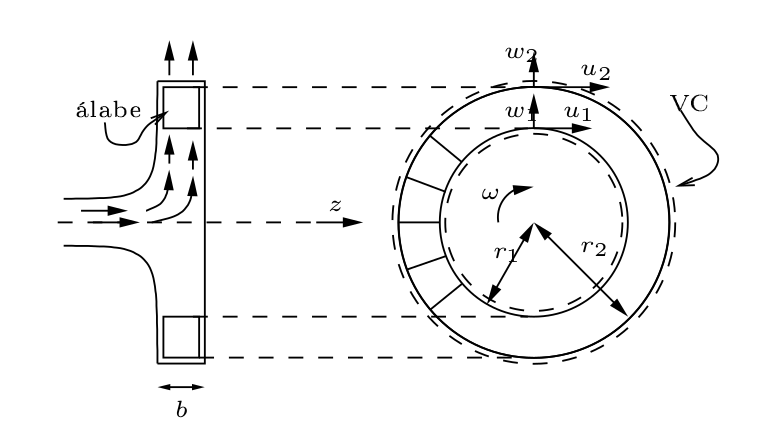
\includegraphics[width=0.5\linewidth]{TeX_files/chapter04-Dinamica/rodete1}
\end{center}

El fluido entra en el VC con una velocidad $\vec{c}_{1}=\vec{w}_{1}+\vec{u}_{1}$
y sale con una velocidad $\vec{c}_{2}=\vec{w}_{2}+\vec{u}_{2}$

Para mantener este flujo, debemos ejercer un momento mecánico sobre
el eje. Por la conservación del momento cinético, este momento será

\[
\vec{M}_{0}=\oint_{SC}\rho\left(\vec{r}\times\vec{c}\right)\vec{c}\cdot\dif\vec{S}=\rho Q\left[\left(\vec{r}_{2}\times\vec{c}_{2}\right)-\left(\vec{r}_{1}\times\vec{c}_{1}\right)\right]
\]

\[
M_{0}=\rho Q\left(r_{2}u_{2}-r_{1}u_{1}\right)
\]

Dado que $u_{1}=\omega r_{1}$ y $u_{2}=\omega r_{2}$, tenemos 
\[
M_{0}=\rho Q\omega\left(r_{2}^{2}-r_{1}^{2}\right)
\]
y la potencia requerida para bombear este fluido será 
\[
P=M_{0}\omega=\rho Q\omega^{2}\left(r_{2}^{2}-r_{1}^{2}\right)
\]


\subsection*{Actividad 1:}
	Realizar el cálculo de la potencia transmitida para un caudal de
	120 l/min de agua, una velocidad angular de 1725 rpm, unos diámetros
	del rodete de 15 cm y 25 cm y una anchura de rodete de 5 cm (constante).

\subsection{El triángulo de velocidades y la ecuación de Euler}


Las bombas, los ventiladores y las turbinas reales son algo más complicadas.
En realidad los álabes no son rectos, excepto para algunos ventiladores.

Centrándonos en el caso de las bombas centrífugas, los álabes suelen
estar inclinados hacia atrás según el sentido de giro. 

\begin{center}
	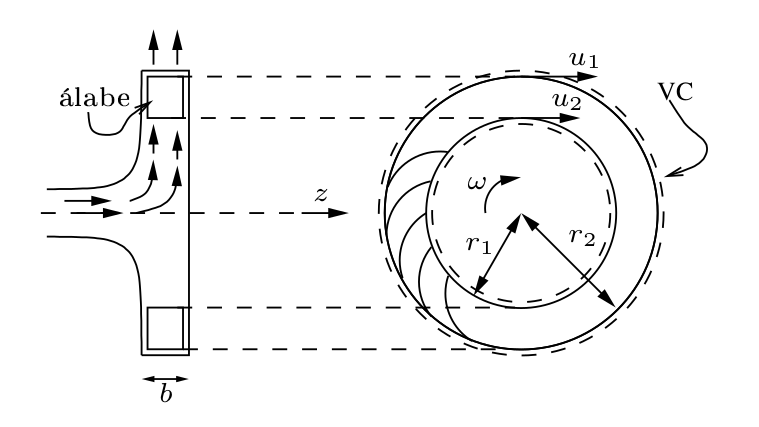
\includegraphics[width=0.5\linewidth]{TeX_files/chapter04-Dinamica/rodete2}
\end{center}


\begin{center}
	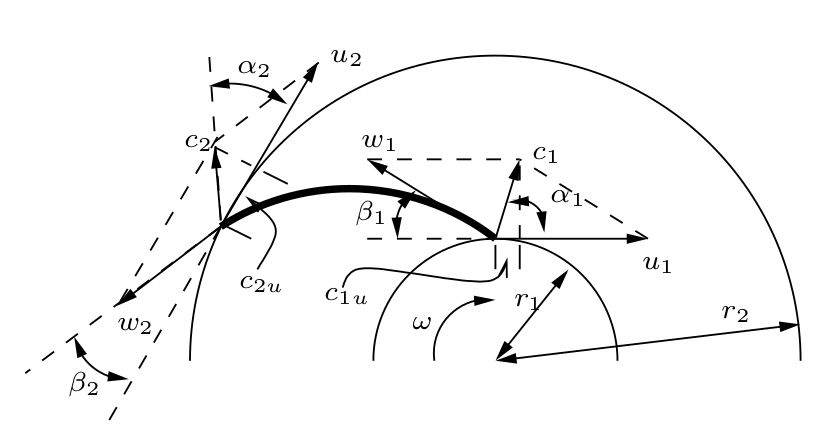
\includegraphics[width=0.5\linewidth]{TeX_files/chapter04-Dinamica/alabe1}
\end{center}

El momento cinético es transportado por la componente de la velocidad
$\vec{c}$ perpendicular al radio, es decir, $c_{1u}$ en la entrada
al VC y $c_{2u}$ en la salida. 

\begin{equation}
	M_{0}=\rho Q\left(r_{2}c_{2u}-r_{1}c_{1u}\right)
\end{equation}



Para calcular $c_{1u}$ y $c_{2u}$, se utilizan los \textcolor{red}{triángulos
de velocidades} 

\begin{center}
	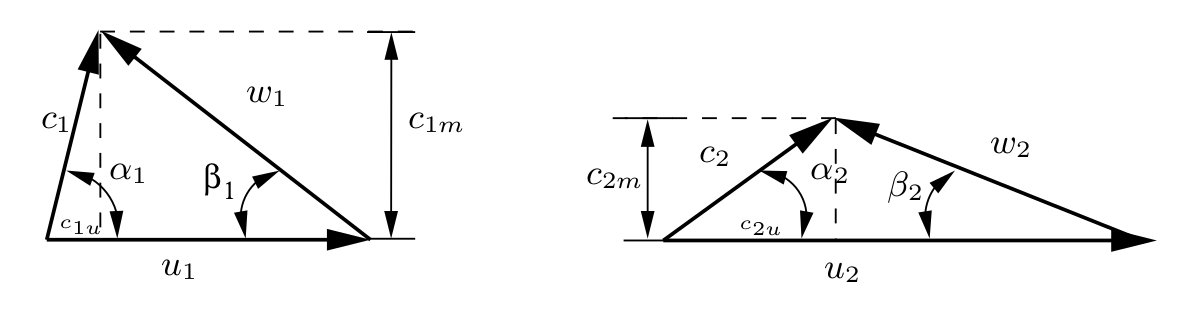
\includegraphics[width=0.7\linewidth]{TeX_files/chapter04-Dinamica/triangulo1}
\end{center}



\begin{equation}
	c_{1u}=u_{1}-\frac{c_{1m}}{\tan\beta_{1}}\qquad c_{2u}=u_{2}-\frac{c_{2m}}{\tan\beta_{2}}
\end{equation}
$c_{1m}$ y $c_{2m}$ se calculan a partir del caudal, 

\begin{equation}
	c_{1m}=\frac{Q}{S_{1}}=\frac{Q}{2\pi r_{1}b_{1}}\qquad c_{2m}=\frac{Q}{S_{2}}=\frac{Q}{2\pi r_{2}b_{2}}
\end{equation}

donde $b_{1}$ y $b_{2}$ son al ancho del rodete en la entrada y
en la salida.



La potencia necesaria para bombear el fluido es 

\begin{equation}
	P=M_{0}\omega=\rho Q\omega\left(r_{2}c_{2u}-r_{1}c_{1u}\right)=\rho Q\left(u_{2}c_{2u}-u_{1}c_{1u}\right)
\end{equation}

y la energia, en forma de altura de fluido, que transmite el rodete
al fluido es 

\begin{equation}
	\boxed{H_{t}=\frac{P}{\rho gQ}=\frac{1}{g}\left(u_{2}c_{2u}-u_{1}c_{1u}\right)}
\end{equation}


Esta es la \textcolor{red}{Ecuación de Euler} para Turbomáquinas,
y el subíndice $t$ indica que la expresión es teórica, ya que hay
muchos aspectos que no se han considerado: 
\begin{itemize}
	\item Número finito de álabes 
	\item Rozamiento en el flujo a través del rodete 
	\item Perfil de velocidad no uniforme en profundidad 
\end{itemize}


\subsection*{Actividad 2:}
	Repetir los cálculos de la Actividad 1, pero ahora los álabes no
	son rectos, sino que son tales que $\beta_{1}=35^{\circ}$ y $\beta_{2}=25^{\circ}$.
	Calcular la energía teórica que da el rodete, en forma de altura de
	fluido. 

\section{Ecuación integral de la conservación de la energía}

	
	Primera ley de la termodinámica para un sistema cerrado: 
	
	\begin{equation}
		\Deriv{E}{t}=\dot{Q}-\dot{W}
	\end{equation}
	
	
	\[
	\begin{array}{cc}
		\dot{Q} & \textrm{: calor transferido al sistema}\\
		\dot{W} & \textrm{: trabajo realizado por el sistema}
	\end{array}
	\]
	
	Aplicando el teorema del transporte de Reynolds al sistema:
	
	\[
	\Deriv{E}{t}=\int_{VC}\dparc{\rho e}{t}\text{d}V+\oint_{SC}\rho e\vec{u}\cdot\text{d}\vec{S}=\dot{Q}-\dot{W}
	\]
	
	donde 
	\[
	e=\underbrace{\frac{1}{2}u^{2}}_{\text{E. cinética}}+\underbrace{\phantom{\frac{1}{2}}gz\phantom{\frac{1}{2}}}_{\text{E. potencial}}+\underbrace{\phantom{\frac{1}{2}}\underline{u}\phantom{\frac{1}{2}}}_{\text{E. interna}}
	\]
	es la energía por unidad de masa.


\subsection{Análisis del trabajo}

	

	\begin{itemize}
		\item trabajo realizado por los esfuerzos normales: 
		\[
		\dot{W}_{n}=-\int_{SC}\tau_{nn}\vec{u}\cdot\text{d}\vec{S}\approx\int_{SC}p\vec{u}\cdot\text{d}\vec{S}
		\]
		
		\item trabajo realizado por los esfuerzos tangenciales: 
		\[
		\dot{W}_{t}=-\int_{SC}\vec{u}\cdot\underbrace{\left(\tens'\cdot\text{d}\vec{S}\right)}_{\vec{\tau}'\text{d}S}=-\int_{SC}\vec{u}\cdot\vec{\tau}'\text{d}S
		\]
		En general, se intenta escoger el $VC$ de forma que $\vec{u}\parallel\text{d}\vec{S}$,
		y, dado que $\vec{\tau}'$ está en $\text{d}S$, $\vec{v}\perp\vec{\tau}'$,
		y $\vec{v}\cdot\vec{\tau}'=0$ (flujos unidimensionales). 
		\item realizado por otros elementos externos, como, p.e., trabajo eléctrico,
		o trabajo mecánico de un eje (agitador, \ldots ). Lo expresamos como
		$\dot{W}_{e}$.
	\end{itemize}

	
	Para un Volumen de Control tal que $\vec{v}\Vert\text{d}\vec{S}$
	en las entradas y salidas, tendremos
	
	\[
	\dot{Q}-\dot{W}_{e}-\oint_{SC}p\vec{u}\cdot\text{d}\vec{S}=\int_{VC}\dparc{\rho e}{t}\text{d}V+\oint_{SC}\rho e\vec{u}\cdot\text{d}\vec{S}
	\]
	
	\[
	\Rightarrow\dot{Q}-\dot{W}_{e}=\int_{VC}\dparc{\rho e}{t}\text{d}V+\oint_{SC}\rho(e+\dfrac{p}{\rho})\vec{u}\cdot\text{d}\vec{S},
	\]
	
	Dado que $\underline{u}+\dfrac{p}{\rho}=h$, la conservación de la
	energía queda 
	

	\begin{equation}
		\boxed{\dot{Q}-\dot{W}_{e}=\int_{VC}\dparc{\rho e}{t}\text{d}V+\oint_{SC}\rho\left(h+gz+\frac{1}{2}u^{2}\right)\vec{u}\cdot\text{d}\vec{S}}
	\end{equation}
	
	
	\subsection*{Actividad 1:}
		¿Porqué no hemos incluido el trabajo realizado por la gravedad en
		$\dot{W}$?

\subsection*{Simplificaciones}
	
	\begin{itemize}
		\item \textcolor{blue}{Flujo permanente :} 
		\[
		\dparc{\rho e}{t}=0
		\]
		en todo el Volumen de Control 
		\item \textcolor{blue}{Propiedades constantes en las superficies de entrada
			(1) y de salida (2) (con flujo unidimensional)}: 
		\[
		\oint_{SC}\rho\left(h+gz+\frac{1}{2}u^{2}\right)\vec{u}\cdot\text{d}\vec{S}=
		\]
		\[
		\rho_{2}\left[h_{2}+gz_{2}+\frac{1}{2}u_{2}^{2}\right]u_{2}S_{2}-\rho_{1}\left[h_{1}+gz_{1}+\frac{1}{2}u_{1}^{2}\right]u_{1}S_{1}
		\]
		\[
		\boxed{\dot{Q}-\dot{W}_{e}=\rho_{2}\left[h_{2}+gz_{2}+\frac{1}{2}u_{2}^{2}\right]u_{2}S_{2}-\rho_{1}\left[h_{1}+gz_{1}+\frac{1}{2}u_{1}^{2}\right]u_{1}S_{1}}
		\]
	\end{itemize}

\subsection{Ecuación de Bernoulli}

	
	Flujo \textcolor{blue}{permanente},\textcolor{blue}{incompresible}
	y \textcolor{blue}{no viscoso}. $\dot{Q}=\dot{W}=0$
	
	\[
	\Rightarrow\rho_{2}\left[h_{2}+gz_{2}+\frac{1}{2}u_{2}^{2}\right]u_{2}S_{2}=\rho_{1}\left[h_{1}+gz_{1}+\frac{1}{2}u_{1}^{2}\right]u_{1}S_{1}
	\]
	
	Dado que $\rho_{2}u_{2}S_{2}=\rho_{1}u_{1}S_{1}=\dot{m}$, tenemos
	\[
	h_{2}+gz_{2}+\frac{1}{2}u_{2}^{2}=h_{1}+gz_{1}+\frac{1}{2}u_{1}^{2}
	\]
	
	Si suponemos también que no hay cambios en la energía interna, 
	\[
	\frac{p_{2}}{\rho}+gz_{2}+\frac{1}{2}u_{2}^{2}=\frac{p_{1}}{\rho}+gz_{1}+\frac{1}{2}u_{1}^{2},
	\]
	es decir, 
	
	\begin{equation}
		\frac{p}{\rho}+gz+\frac{1}{2}u^{2}=cte\quad\text{sobre una línea de corriente}
	\end{equation}
	
	
	Este es la conocida como \textcolor{red}{Ecuación de Bernoulli}.



	
	\subsection*{Actividad 2:}
		Una pareja que vive en una casa en la montaña decide aprovechar el
		arroyo de cerca de su casa para generar la energia necesaria para
		su vivienda. Compran una turbina en eBay y estiman que poniendo una
		presa podrían conseguir una altura en la entrada de la turbina de
		unos 4 metros. El caudal del arroyo es de unos 800 litros por segundo.
		Si en la salida de la turbina la velocidad del agua será de 3,6 m/s,
		estimad la potencia que podrían generar, menospreciando pérdidas por
		rozamiento.


\section{Ecuación diferencial de la conservación de la energía}

	
	$\vec{g}$ : fuerzas másicas
	
	Partiendo de la forma general de la conservación de la energia en
	un VC 
	\[
	\dot{Q}+\int_{VC}\vec{g}\cdot\vec{u}\rho\,\dif V+\oint_{SC}\vec{u}\cdot\left(\tens\cdot\dif\vec{S}\right)=\int_{VC}\dparc{\rho e}{t}\,\dif V+\oint_{SC}\rho e\vec{u}\cdot\dif\vec{S}
	\]
	donde $\tens$ incluye la diagonal y $e$ no incluye el término $gz$ 
	
	
	$\dot{Q}$ puede ser debido o bien a un flujo de calor ($\vec{q}$)
	a través de la $SC$ o bien a una producción de energía en el interior
	del $VC$ ($s$, que tiene unidades de W/kg). 
	\[
	\dot{Q=}-\oint_{SC}\vec{q}\cdot\dif\vec{S}+\int_{VC}s\rho\,\dif V
	\]
	

	
	Usando el Teorema de Gauss sobre las tres $SC$, queda 
	\begin{eqnarray*}
		-\int_{VC}\vec{\nabla}\vec{q}\dif V+\int_{VC}s\rho\,\dif V+\int_{VC}\vec{g}\cdot\vec{u}\rho\,\dif V+\int_{VC}\vec{\nabla}\left(\tens\cdot\vec{u}\right)\dif V=\\
		=\int_{VC}\dparc{\rho e}{t}\,\dif V+\int_{VC}\vec{\nabla}\cdot\left(\rho e\vec{u}\right)\dif V
	\end{eqnarray*}
	
	Si lo reescribimos en forma de componentes, usando el convenio de
	doble índice, y en una sola integral, obtenemos 
	\[
	\int_{VC}\left[-\dparc{q_{i}}{x_{i}}+\rho s+\rho g_{i}u_{i}+\dparc{\tau_{ij}u_{i}}{x_{j}}-\dparc{e\rho u_{i}}{x_{i}}+\dparc{\rho e}{t}\right]\dif V=0
	\]
	Dado que esto ha de ser cierto para todo $VC$, el integrando debe
	ser nulo, 
	\[
	-\dparc{q_{i}}{x_{i}}+\rho s+\rho g_{i}u_{i}+\dparc{\tau_{ij}u_{i}}{x_{j}}-\dparc{e\rho u_{i}}{x_{i}}+\dparc{\rho e}{t}=0
	\]
	

	
	Para simplificar esta expresión expandimos en primer lugar todas las
	derivadas, usando $e=\underline{u}+\frac{1}{2}u^{2}$. 
	\[
	-\dparc{q_{i}}{x_{i}}+\rho s+\rho g_{i}u_{i}+\tau_{ij}\dparc{u_{i}}{x_{j}}+u_{i}\dparc{\tau_{ij}}{x_{j}}=
	\]
	\[
	=\rho u_{i}\dparc{}{x_{i}}\left(\frac{u^{2}}{2}\right)+\frac{u^{2}}{2}\dparc{}{x_{i}}\left(\rho u_{i}\right)+\underline{u}\rho\dparc{u_{i}}{x_{i}}+\underline{u}u_{i}\dparc{\rho}{x_{i}}+\rho u_{i}\dparc{\underline{u}}{x_{i}}+
	\]
	\[
	+\rho\dparc{\phantom{}}{t}\left(\frac{u^{2}}{2}\right)+\left(\frac{u^{2}}{2}\right)\dparc{\rho}{t}+\underline{u}\dparc{\rho}{t}+\rho\dparc{\underline{u}}{t}
	\]
	

	
	Reordenando términos, tenemos 
	\[
	\underbrace{u_{i}\underbrace{\left[\dparc{\tau_{ij}}{x_{j}}+\rho g_{i}\right]}_{\rho\Deriv{u_{i}}{t}}}_{=\frac{\rho}{2}\Deriv{u^{2}}{t}}+\tau_{ij}\dparc{u_{i}}{x_{j}}-\dparc{q_{i}}{x_{i}}+\rho s=
	\]
	
	\[
	=\frac{\rho}{2}\underbrace{\left[\dparc{u^{2}}{t}+u_{i}\dparc{u^{2}}{x_{i}}\right]}_{=\Deriv{u^{2}}{t}}+\frac{u^{2}}{2}\underbrace{\left[\dparc{\rho u_{i}}{x_{i}}+\dparc{\rho}{t}\right]}_{=0}+\rho\underbrace{\left[\dparc{\underline{u}}{t}+v_{i}\dparc{\underline{u}}{x_{i}}\right]}_{\Deriv{\underline{u}}{t}}+
	\]
	
	\[
	+\underline{u}\underbrace{\left[\dparc{\rho}{t}+u_{i}\dparc{\rho}{x_{i}}\right]}_{\Deriv{\rho}{t}}+\underline{u}\rho\dparc{u_{i}}{x_{i}}
	\]
	
	
	\ldots{} y simplificando, 
	\[
	\tau_{ij}\dparc{u_{i}}{x_{j}}-\dparc{q_{i}}{x_{i}}+\rho s=\rho\Deriv{\underline{u}}{t}+\underline{u}\underbrace{\left[\Deriv{\rho}{t}+\rho\dparc{u_{i}}{x_{i}}\right]}_{=0}
	\]
	
	
	
	\begin{equation}
		\boxed{\tau_{ij}\dparc{u_{i}}{x_{j}}-\dparc{q_{i}}{x_{i}}+\rho s=\rho\Deriv{\underline{u}}{t}}
	\end{equation}
	
	
	
	Si ahora usamos la ley de Fourier 
	\[
	q_{i}=-k\dparc{T}{x_{i}}
	\]
	y la descomposición $\tau_{ij}=-p\delta_{ij}+\tau'_{ij}$, como hicimos
	con la conservación de cantidad de movimiento, 
	\[
	-p\dparc{u_{i}}{x_{j}}\delta_{ij}+\underbrace{\tau'_{ij}\dparc{u_{i}}{x_{j}}}_{\text{función disipación }\Phi}+\dparc{\phantom{}}{x_{i}}\left(k\dparc{T}{x_{i}}\right)+\rho s=\rho\Deriv{\underline{u}}{t}
	\]
	
	\begin{equation}
		\rho\Deriv{\underline{u}}{t}=\rho\left(\dparc{\underline{u}}{t}+u_{i}\dparc{\underline{u}}{x_{i}}\right)=-p\dparc{u_{i}}{x_{i}}+\Phi+\rho s+\dparc{\phantom{}}{x_{i}}\left(k\dparc{T}{x_{i}}\right)
	\end{equation}
	
	
	Para un fluido newtoniano, 
	\[
	\Phi=\mu\sum_{ij}\left(\dparc{u_{i}}{x_{j}}+\dparc{u_{j}}{x_{i}}\right)^{2}
	\]

\section{Derivación de la Ecuación de Bernoulli a partir de la Ecuación de Euler}
	
	Integramos la Ecuación de Euler 
	\[
	\rho\,\dparc{\vec{u}}{t}+\rho\left(\vec{u}\cdot\vec{\nabla}\right)\vec{u}=\rho\vec{g}-\vec{\nabla}p
	\]
	sobre una línea de corriente. La coordenada $s$ es la posición sobre
	la línea, y, dado que la velocidad debe ser tangente a la línea de
	corriente, sólo hay una ecuación de Euler para el módulo de $\vec{u}$,
	\[
	\dparc{u}{t}+u\dparc{u}{s}=-\frac{1}{\rho}\dparc{p}{s}-g\dparc{z}{s}
	\]
	
	Consideremos flujo estacionario, 
	\[
	u\dparc{u}{s}=-\frac{1}{\rho}\dparc{p}{s}-g\dparc{z}{s}
	\]
	
	
	Si una partícula de fluido se mueve una distancia $\dif s$ sobre
	la línea de corriente, tendremos 
	\begin{eqnarray*}
		\dparc{u}{s}\dif s & = & \dif u\\
		\dparc{p}{s}\dif s & = & \dif p\\
		\dparc{z}{s}\dif s & = & \dif z
	\end{eqnarray*}
	de forma que 
	\[
	u\dif u=-\frac{1}{\rho}\dif p-g\dif z\;\Rightarrow\;u\dif u+\frac{1}{\rho}\dif p+g\dif z=0
	\]
	\[
	\Rightarrow\;\frac{1}{2}u^{2}+\int\frac{\dif p}{\rho}+gz=\text{cte}
	\]
	y, si el fluido es incompresible, obtenemos la ecuación de Bernoulli
	\[
	\boxed{\frac{1}{2}u^{2}+\frac{p}{\rho}+gz=\text{cte}}
	\]
	


\section{Presión estática, dinámica y de remanso}

	
	Un \textcolor{red}{tubo de Pitot} es una sonda de diámetro muy pequeño,
	que se usa para medir la velocidad de un flujo. En la figura se muestra
	una en ángulo recto, usada para medir la velocidad en un canal. 
	
\begin{center}
	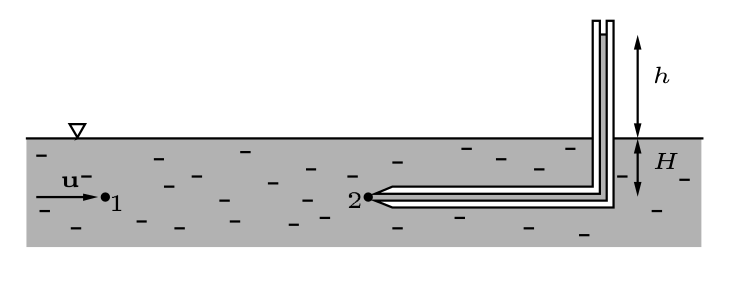
\includegraphics[width=0.5\linewidth]{TeX_files/chapter04-Dinamica/pitot1}
\end{center}

	
	
	El fluido penetra en la sonda y sube por el tubo hasta una altura
	$h$ por encima del nivel del canal. Esta altura es tal que la presión
	que crea en la boca del tubo contrarresta la energia que lleva el
	fluido. El punto 2, justo delante de la boca del tubo, recibe el nombre
	de \textcolor{green}{punto de estancamiento o de remanso}. En este
	punto, la velocidad del fluido es nula. El punto 1 está lo suficientemente
	lejos como para considerar que no está afectado por la sonda.
	
	Un tubo de Pitot mide la presión en el punto 2, es decir, la \textcolor{red}{presión
		de remanso} o \textcolor{red}{presión total}.
	
	Si aplicamos Bernoulli entre los puntos 1 y 2, que están en la misma
	línea de corriente, 
	\[
	\rho\,\frac{v_{1}^{2}}{2}+p_{1}=p_{2}=\rho g(H+h)
	\]
	
	Dado que $p_{1}=\rho gH$, obtenemos, de forma muy sencilla, 
	\[
	\frac{v_{1}^{2}}{2}=gh\;\Rightarrow\;v_{1}=v=\sqrt{2gh}
	\]
	
La presión total se compone de \textcolor{red}{presión estática} $p$
y \textcolor{red}{presión dinámica} $\frac{\rho v^{2}}{2}$. 

Con un tubo de Pitot podemos medir la presión dinámica y, por tanto,
la velocidad, si conocemos la presión estática (como era el caso del
canal abierto). 

Si no es el caso, utilizamos un \textcolor{green}{tubo de Pitot estático}
o \textcolor{green}{tubo de Prandtl}.

\begin{tabular}{cc}
	\begin{minipage}[c]{0.4\textwidth}%
		\begin{center}
			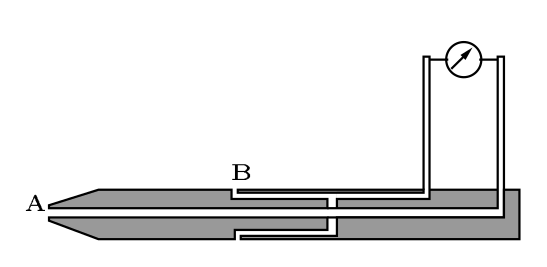
\includegraphics[width=0.7\linewidth]{TeX_files/chapter04-Dinamica/pitot2}
		\end{center}
		
		\[
		v=\sqrt{\frac{2(p_{A}-p_{B})}{\rho}}
		\]
		%
	\end{minipage} & %
	\begin{minipage}[c]{0.4\textwidth}%
		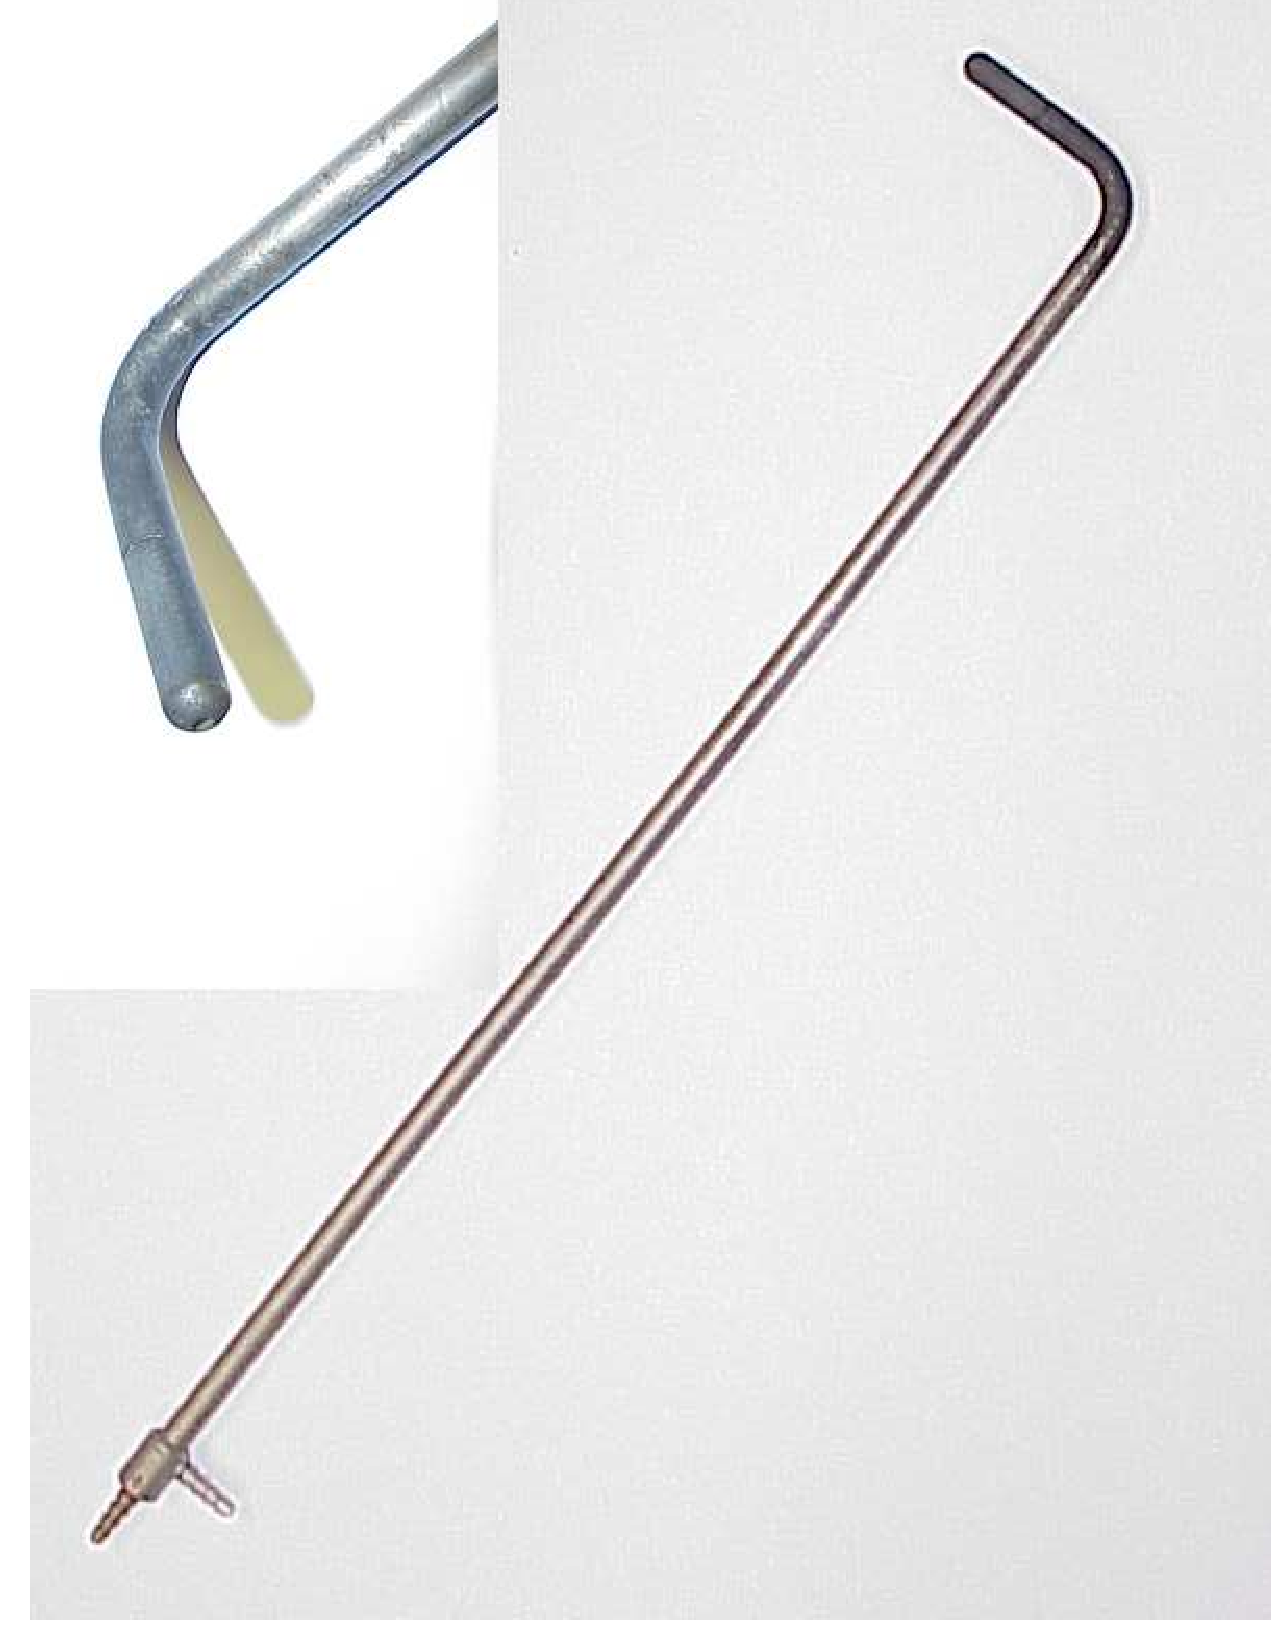
\includegraphics[clip,width=0.8\textwidth,angle=270]{TeX_files/chapter04-Dinamica/prandtl} %
	\end{minipage}\tabularnewline
\end{tabular}
\subsection{Tubo de Venturi}
	
	\begin{tabular}{cc}
		\begin{minipage}[c]{0.4\textwidth}%
			\begin{center}
				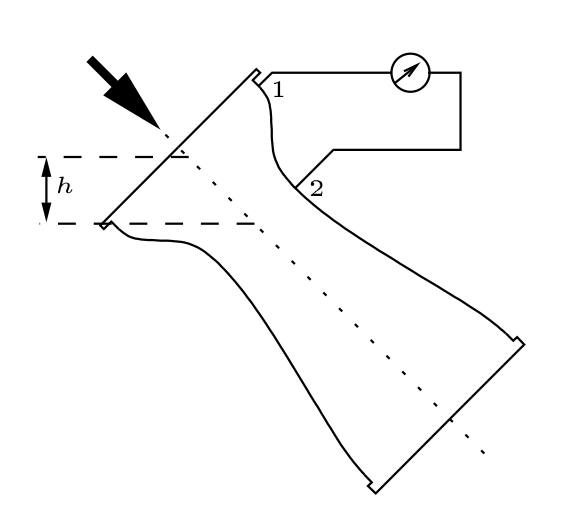
\includegraphics[width=\linewidth]{TeX_files/chapter04-Dinamica/venturi}
			\end{center}
		\end{minipage} & %
		\begin{minipage}[c]{0.4\textwidth}%
			
			\begin{align*}
				\frac{1}{2}\rho u_{1}^{2}+p_{1}+\rho gh=\frac{1}{2}\rho u_{2}^{2}+p_{2}\\
				\Rightarrow\frac{1}{2}\left(u_{2}^{2}-u_{1}^{2}\right)=\Delta p+\rho gh
			\end{align*}
			
			\[
			u_{1}=u_{2}\left(\frac{D_{2}}{D_{1}}\right)^{2}=u_{2}\beta^{2}
			\]
			
			\begin{align*}
				\frac{1}{2}\rho\left[1-\beta^{4}\right]u_{2}^{2}=\Delta p+\rho gh\\
				\Rightarrow\quad u_{2}=\sqrt{\frac{2\left(\Delta p+\rho gh\right)}{\rho\left[1-\beta^{4}\right]}}
			\end{align*}
			%
		\end{minipage}\tabularnewline
	\end{tabular}

	
	El caudal es $Q=u_{2}S_{2}$ . Éste caudal es teórico. El real se
	calcula multiplicando por un \textcolor{red}{coeficiente de descarga}
	$C_{d}$ que se obtiene por calibración. Normalmente $C_{d}\approx0.95\div1.0$.
	
	El caudal es, entonces, 
	\[
	Q_{r}=u_{2r}S_{2}=C_{d}S_{2}\sqrt{\frac{2\left(\Delta p+\rho gh\right)}{\rho\left[1-\beta^{4}\right]}}
	\]
	
	\subsection*{Actividad 1:}
		En un tubo de Venturi, de diámetros 200 mm y 160 mm, instalado horizontalmente,
		se mide una diferencia de presión de 25 mm de mercurio en una instalación
		de agua. ¿Cuál és el caudal teórico de agua que circula?

\subsection{Diafragma}
	
	La idea del diafragma es la misma que la del tubo de Venturi, pero
	carece de la sección de ampliación de la sección corriente abajo.
	Esto hace que el dispositivo sea más barato, y el montaje más sencillo.
	
	La ecuación para el caudal es la misma que para el tubo de Venturi,
	pero $C_{d}$ es generalmente menor. 
	
\begin{center}
	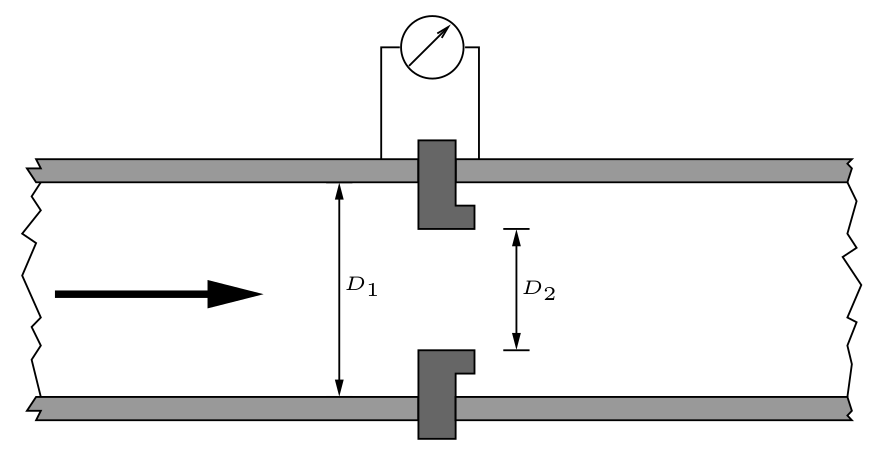
\includegraphics[width=0.7\linewidth]{TeX_files/chapter04-Dinamica/diafragma}
\end{center}

	


\subsection{Vaciado de un depósito}
	
	\begin{tabular}{cc}
		\begin{minipage}[c]{0.4\textwidth}%
			\begin{center}
				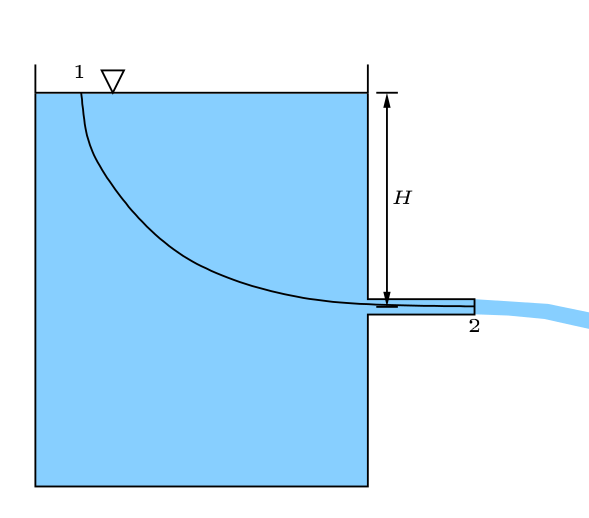
\includegraphics[width=\linewidth]{TeX_files/chapter04-Dinamica/deposito}
			\end{center}
		\end{minipage} & %
		\begin{minipage}[c]{0.5\textwidth}%
			Menospreciando la viscosidad, 
			\[
			\frac{1}{2}\rho u_{1}^{2}+p_{1}+\rho gH=\frac{1}{2}\rho u_{2}^{2}+p_{2}.
			\]
			
			Dado que tanto el punto 1 como el 2 están abiertos, $p_{1}=p_{2}=0$.
			Por otro lado, si suponemos que $S_{1}\gg S_{2}$, entonces $u_{1}^{2}\approx0$,
			\[
			\rho gH=\frac{1}{2}\rho u_{2}^{2}\;\Rightarrow\;\underbrace{u_{2}=\sqrt{2gH}}_{\text{Ec. de Torricelli}},
			\]
			y 
			\[
			Q_{t}=u_{2}S_{2}\sqrt{2gH}\qquad\text{(teórico)}
			\]
			%
		\end{minipage}\tabularnewline
	\end{tabular}
	
	\begin{tabular}{l>{\raggedright}p{0.7\textwidth}}
		\begin{minipage}[c]{0.4\textwidth}%
			\begin{center}
				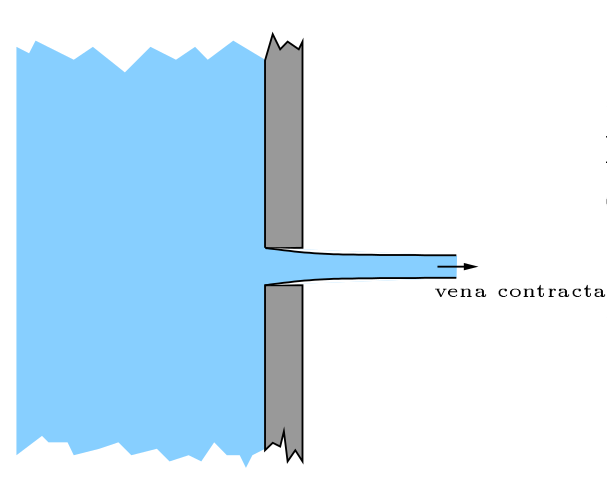
\includegraphics[width=\linewidth]{TeX_files/chapter04-Dinamica/orificio}
			\end{center}
		\end{minipage} & %
		\begin{minipage}[c]{0.6\textwidth}%
			Si la descarga se realiza a través de un orificio, se produce una
			vena contracta de forma que $S_{c}\lessapprox S_{2}$. 
			\[
			S_{c}=C_{c}S_{2}
			\]
			$C_{c}$ : \textcolor{blue}{Coeficiente de contracción} $\lessapprox1.0$
			
			Por otro lado, debido al rozamiento, la velocidad disminuye, 
			\[
			u_{c}=C_{v}u_{2}
			\]
			$C_{v}$ : \textcolor{blue}{Coeficiente de velocidad} $\lessapprox1.0$
			
			\begin{align*}
				Q=u_{c}S_{c}=C_{c}C_{v}S_{2}\sqrt{2gH}\\
				=C_{d}S_{2}\sqrt{2gH}
			\end{align*}
			$C_{d}$ : \textcolor{blue}{Coeficiente de descarga} %
		\end{minipage}\tabularnewline
	\end{tabular}

	
	\subsection*{Ejemplo: Cálculo de tiempo de vaciado de un depósito.}
		\[
		Q=C_{d}S_{2}\sqrt{\frac{2gH}{1-\left(\frac{S_{2}}{S_{1}}\right)^{2}}}=\frac{C_{d}S_{2}}{\sqrt{1-\left(\frac{S_{2}}{S_{1}}\right)^{2}}}\sqrt{2gH}
		\]
		\[
		u_{1}=\frac{Q}{S_{1}}=\frac{C_{d}\frac{S_{2}}{S_{1}}}{\sqrt{1-\left(\frac{S_{2}}{S_{1}}\right)^{2}}}\sqrt{2gH}=\underbrace{\frac{C_{d}\sqrt{2g}}{\sqrt{\left(\frac{S_{1}}{S_{2}}\right)^{2}-1}}}_{\alpha}\sqrt{H}
		\]
		\[
		u_{1}=-\deriv{H}{t}=\alpha H^{1/2}\Rightarrow\frac{\dif H}{H^{1/2}}=-\alpha\dif t\Rightarrow\int_{H_{0}}^{0}H^{-1/2}\dif H=-\alpha\int_{0}^{t}\dif t
		\]
		\[
		2\left.H^{1/2}\right]_{H_{0}}^{0}=-\alpha t\;\Rightarrow\;t=\frac{2}{\alpha}\sqrt{H}=\frac{2\sqrt{\left(\frac{S_{1}}{S_{2}}\right)^{2}-1}}{C_{d}\sqrt{2g}}\sqrt{H}
		\]

	
	\subsection*{Actividad 2:}
		Estima el tiempo que tarda en vaciarse una botella de agua de 1.5
		litros puesta boca abajo. ¿Porqué en realidad tarda mucho más?

	
	\subsection*{Actividad 3:}
		¿Cómo se modifican los cálculos si el depósito no es cilindrico (p.e.,
		un embudo)?

	
\chapter{Flujo con viscosidad dominante}

	
	\begin{itemize}
		\item Si el término de fuerzas viscosas $\mu\triangle\vec{u}$ no es menospreciable
		en la ecuación de Navier-Stokes, ésta puede ser complicada de resolver.
		\item No existe una solución general de la ecuación de Navier-Stokes.
		\item La razón principal es la no-linealidad impuesta por la aceleración
		convectiva en la interpretación euleriana del flujo.
		\item Solo en el caso de geometrías muy sencillas y flujo lento es posible
		encontrar una solución analítica. En estas configuraciones de flujo,
		se produce de una forma u otra una  \textit{linealización}
		de las ecuaciones de Navier-Stokes.
		\item A parte de estos flujos sencillos, existen multitud de resoluciones
		numéricas con geometrías más complicadas y multitud de datos experimentales.
		\item En este tema de flujo viscoso vamos a estudiar algunos de estos flujos
		sencillos que pueden ser analizados de forma analítica. Estos flujos
		estan caracterizados por un número de Reynolds bajo.
		\item Todos los flujos estudiados serán considerados incompresibles, y no
		tendremos en cuenta otros efectos que pudiesen causar una posible
		variación de la densidad. Es decir, no consideraremos las ecuaciones
		de balance de la energía.
	\end{itemize}

\section{Ecuaciones y condiciones de contorno}

	
	Los flujos de fluidos ideales se caracterizan por que, dado que no
	hay viscosidad, no existe la condición de  \textit{no deslizamiento}
	en contacto con paredes sólidas.
	
			Los flujos de fluidos viscosos han de cumplir esta condición de contorno,
			de forma que 
			\[
			\vec{u}=\vec{u}_{s}
			\]
			en los puntos en contacto con un sólido, donde $\vec{v}_{s}$ es
			la velocidad del sólido. A este tipo de condiciones de contorno se
			le denominan \textcolor{blue}{condiciones de contorno de Dirichlet} %

\begin{center}
	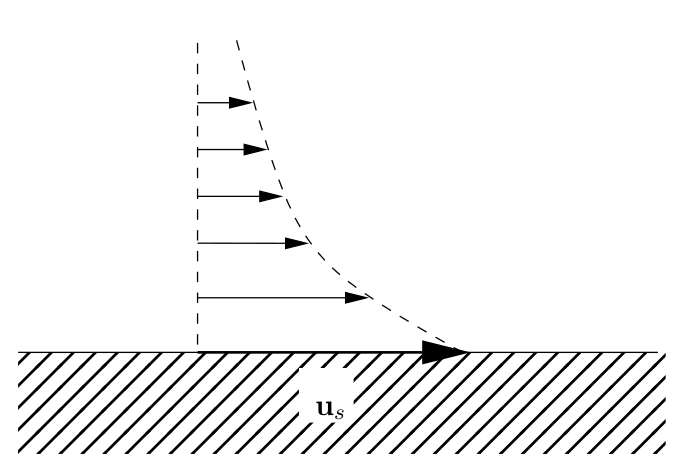
\includegraphics[width=0.5\linewidth]{TeX_files/chapter05-FlujoViscoco/no-slip}
\end{center}


			Otra condición que se ha de cumplir en ciertos puntos es la de esfuerzo
			tangencial nulo. 
			\[
			\tau_{nt}=\mu\dparc{u_{t}}{n}=0.
			\]
			Esta es una \textcolor{blue}{condición de contorno de Neumann}, y
			se cumple, por ejemplo, en planos de simetria y en superficies libres,
			cuando el efecto de la tensión superficial no es importante. %
\begin{center}
	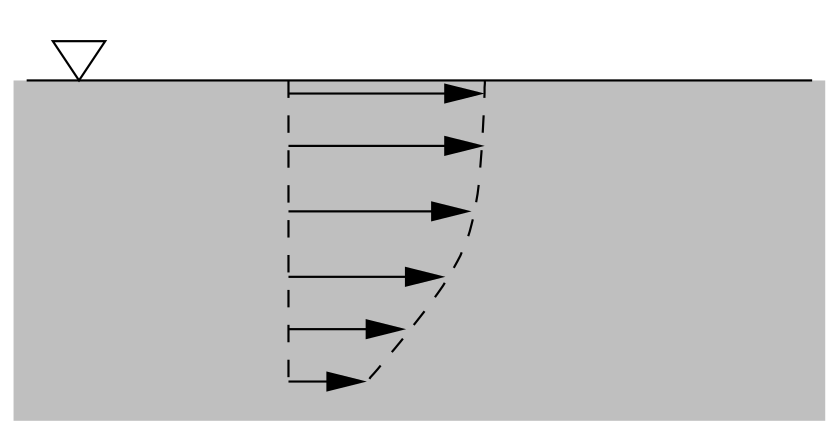
\includegraphics[width=0.5\linewidth]{TeX_files/chapter05-FlujoViscoco/sup_libre}
\end{center}

	
	Todos estos flujos estan descritos por : 
	\begin{itemize}
		\item \textbf{La ecuación de continuidad} 
		
		\begin{equation}
			\vec{\nabla}\cdot\vec{u}=0
		\end{equation}
		
		
		\item \textbf{Las ecuaciones de Navier-Stokes} 
		
		\begin{equation}
			\dparc{\vec{u}}{t}+\left(\vec{u}\cdot\vec{\nabla}\right)\vec{u}=-\dfrac{1}{\rho}\vec{\nabla}p\ +\vec{g}+\dfrac{\mu}{\rho}\triangle\vec{u}
		\end{equation}
		
		
		\item En muchas ocasiones es interesante, o incluso imprescindible, utilizar
		coordenadas polares en flujos bidimensionales y cilíndricas o esféricas
		en flujos tridimensionales.
		\item Las coordenadas esféricas no serán usadas en el presente curso. Las
		ecuaciones de continuidad y Navier-Stokes en coordenadas cilíndricas
		serán vistas en la siguiente sesión.
	\end{itemize}

\section{Flujo entre placas planas paralelas}
	
	\subsection{Flujo entre placas planas paralelas con movimiento relativo
	}
	
	\begin{center}
		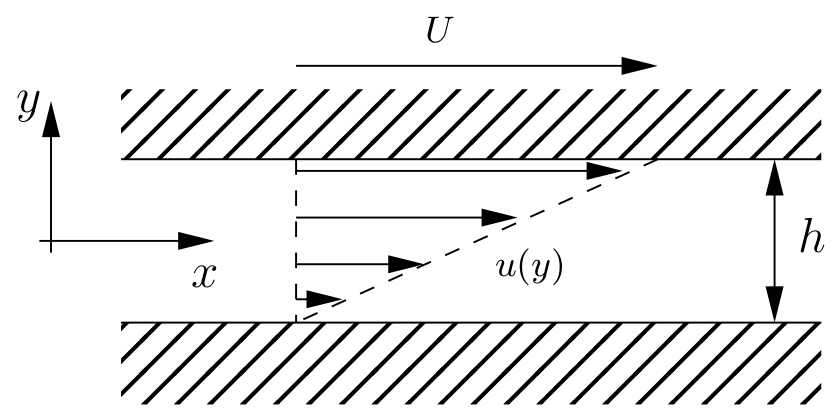
\includegraphics[width=0.5\linewidth]{TeX_files/chapter05-FlujoViscoco/placas1}
	\end{center}
	
			Si las placas son muy grandes en comparación con $h$, el flujo sólo
			tiene dirección $x$, $v=w=0$. El flujo es bidimensional, 
			
			\begin{equation}
				\dparc{}{z}=0
			\end{equation}
			
		
	
	Consideraremos que no hay ningún gradiente de presión, el flujo es
	estacionario, y no afecta la gravedad.
	
	La ecuación de continuidad es 
	
\begin{equation}
		\dparc{u}{x}+\dparc{v}{y}+\dparc{w}{z}=0\,\Rightarrow\,\dparc{u}{x}=0
\end{equation}
	
	, es decir, la velocidad $u$ sólo puede depender de $y$.
	
	Sólo hay una ecuación de Navier-Stokes, la correpondiente a $u$,
	\[
	\underbrace{\dparc{u}{t}}_{\binom{=0}{\text{(est.)}}}+\underbrace{u\dparc{u}{x}}_{\binom{=0}{u(y)}}+\underbrace{v\dparc{u}{y}}_{\binom{=0}{v=0}}=-\underbrace{\frac{1}{\rho}\dparc{p}{x}}_{\binom{=0}{\text{no}\,\vec{\nabla}p}}+\frac{\mu}{\rho}\Bigl(\underbrace{\dparcsec{u}{x}}_{\binom{=0}{u(y)}}+\dparcsec{u}{y}\Bigr)
	\]
	que se reduce a 
	\[
	\derivsec{u}{y}=0\,\Rightarrow\,u=C_{1}y+C_{2}.
	\]
	
	Aplicando las condiciones de contorno \textrm{$u=U\,\text{en}\,y=\frac{h}{2}$
		y $u=0\,\text{en}\,y=-\frac{h}{2}$,} se obtiene 
	\[
	\left.\begin{array}{l}
		U=C_{1}\left(\dfrac{h}{2}\right)+C_{2}\\
		0=C_{1}\left(-\dfrac{h}{2}\right)+C_{2}
	\end{array}\right\} \,\Rightarrow C_{1}=\dfrac{U}{h}\,;\,C_{2}=\dfrac{U}{2}\;\Rightarrow\;\boxed{u=\frac{U}{h}y+\frac{U}{2}}
	\]
	
	
	\subsection{Flujo entre placas planas fijas con gradiente de presión	}
	
	\begin{center}
		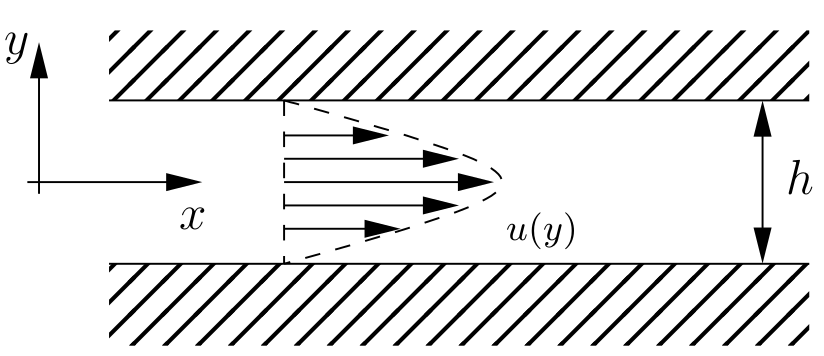
\includegraphics[width=0.5\linewidth]{TeX_files/chapter05-FlujoViscoco/placas2}
	\end{center}
	

			De nuevo el flujo es bidimensional, y $u$ sólo depende de $y$.
			
			La ecuación de Navier-Stokes para $u$ se reduce a 
			
\begin{equation}
				\mu\derivsec{u}{y}=\dparc{p}{x}
\end{equation}
			
			%

	
	Por otro lado, las ecuaciones de Navier-Stokes para las direcciones
	$y$ y $z$ llevan a $\dparc{p}{y}=\dparc{p}{z}=0$. Es decir, $p=p(x)$.
	
	Esto implica que 
	\[
	\mu\derivsec{u}{y}=\deriv{p}{x}=\text{const}<0
	\]
	
	\[
	u(y)=\frac{1}{2\mu}\deriv{p}{x}y^{2}+C_{1}y+C_{2}
	\]

	Las condiciones de contorno son 
\begin{eqnarray*}
	u=0\, & \text{en} & \,y=\frac{h}{2}\\
	u=0\, & \text{en} & \,y=-\frac{h}{2}
\end{eqnarray*}
que llevan a 
\[
\left.\begin{array}{l}
	0=\frac{1}{2\mu}\deriv{p}{x}\left(\frac{h}{2}\right)^{2}+C_{1}\left(\frac{h}{2}\right)+C_{2}\\
	0=\frac{1}{2\mu}\deriv{p}{x}\left(-\frac{h}{2}\right)^{2}+C_{1}\left(-\frac{h}{2}\right)+C_{2}
\end{array}\right\} \Rightarrow\,C_{1}=0\,;\,C_{2}=-\frac{1}{2\mu}\deriv{p}{x}\left(\frac{h}{2}\right)^{2}
\]


\begin{equation}
	\boxed{u(y)=\frac{1}{2\mu}\deriv{p}{x}\left[y^{2}-\left(\frac{h}{2}\right)^{2}\right]}
\end{equation}


Recordemos que la parte anisotrópica del tensor de tensiones (no se
considera la presión) es de la forma
\[
\vec{\vec{\tau}}^{\prime}=2\mu\left(\vec{\nabla}\text{\ensuremath{\vec{u}}}\right)^{S}=\mu\left(\dparc{v}{x}+\dparc{u}{y}\right)\approx\mu\dparc{u}{y}
\]

\subsection*{Actividad 1:}
Calcular la velocidad máxima del flujo y el esfuerzo tangencial en las placas.


\subsection*{Actividad 2:}
Calcular el perfil de velocidades en el caso de dos placas con movimiento
relativo y gradiente de presiones.
	
\section{Ecuaciones de continuidad y Navier-Stokes en coordenadas cilíndricas}

\begin{center}
	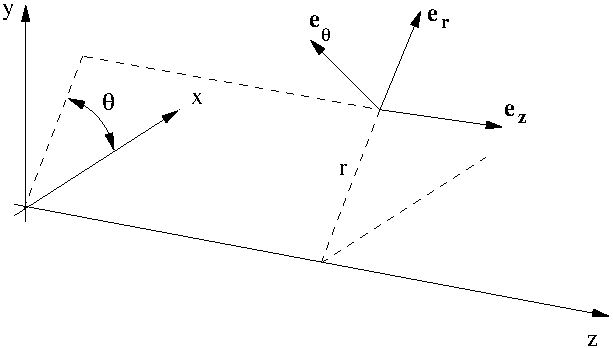
\includegraphics[width=0.5\linewidth]{TeX_files/chapter05-FlujoViscoco/Figures/cilindricas.pdf}
\end{center}

	
	Los operadores diferenciales son definidos de nuevo según :
	
	$\phi$ : escalar ; $\vec{A}$ : vector 
		\[
		\vec{\nabla}\phi=\dparc{\phi}{r}\vec{e}_{r}+\frac{1}{r}\dparc{\phi}{\theta}\vec{e}_{\theta}+\dparc{\phi}{z}\vec{e}_{z}
		\]
		
		\[
		\vec{\nabla}\cdot\vec{A}=\frac{1}{r}\dparc{\phantom{r}}{r}\left(rA_{r}\right)+\frac{1}{r}\dparc{A_{\theta}}{\theta}+\dparc{A_{z}}{z}
		\]
	
		\[
		\begin{aligned}\vec{A}\cdot\vec{\nabla}=A_{r}\dparc{}{r}+\frac{1}{r}A_{\theta}\dparc{}{\theta}+A_{z}\dparc{}{z}\\
			\triangle=\vec{\nabla}^{2}=\frac{1}{r}\dparc{}{r}\left(r\dparc{}{r}\right)+\frac{1}{r^{2}}\dparcsec{}{\theta}+\dparcsec{}{z}\\
			\begin{split}\vec{\nabla}\times\vec{A}=\left(\frac{1}{r}\dparc{A_{z}}{\theta}-\dparc{A_{\theta}}{z}\right)\vec{e}_{r}+\left(\dparc{A_{r}}{\theta}-\dparc{A_{z}}{r}\right)\vec{e}_{\theta}+\left(\frac{1}{r}\dparc{\phantom{r}}{r}\left(rA_{\theta}\right)-\frac{1}{r}\dparc{A_{r}}{\theta}\right)\vec{e}_{z}\end{split}
		\end{aligned}
		\]
	
	El tensor divergencia, en coordenadas cilíndricas, es
	\[
	\nabla\vec{A}=\begin{pmatrix}\dparc{A_{r}}{r} & \dparc{A_{\theta}}{r} & \dparc{A_{z}}{r}\\
		\left(\frac{1}{r}\dparc{A_{r}}{\theta}-\frac{A_{\theta}}{r}\right) & \left(\frac{1}{r}\dparc{A_{\theta}}{\theta}+\frac{A_{r}}{r}\right) & \frac{1}{r}\dparc{A_{z}}{\theta}\\
		\dparc{A_{r}}{z} & \dparc{A_{\theta}}{z} & \dparc{A_{z}}{z}
	\end{pmatrix}
	\]
	
	
	Las ecuaciones en coordenadas cilíndricas son:
	
	\textbf{Continuidad :} 
	
\begin{equation}
		\boxed{\frac{1}{r}\dparc{}{r}(ru_{r})+\frac{1}{r}\dparc{u_{\theta}}{\theta}+\dparc{u_{z}}{z}=0}
\end{equation}
	
	
	\textbf{Navier-Stokes :} {\small{}
		
		\begin{equation}
			\boxed{\begin{array}{ll}
				r\,: & \qquad\dparc{u_{r}}{t}+\bigl(\vec{u}\cdot\vec{\nabla}\bigr)u_{r}-\frac{1}{r}u_{\theta}^{2}=-\frac{1}{\rho}\dparc{p}{r}+g_{r}+\frac{\mu}{\rho}\bigl(\triangle u_{r}-\frac{u_{r}}{r^{2}}-\frac{2}{r^{2}}\dparc{u_{\theta}}{\theta}\bigr)\\
				\theta\,: & \qquad\dparc{u_{\theta}}{t}+\bigl(\vec{u}\cdot\vec{\nabla}\bigr)u_{\theta}+\frac{1}{r}u_{r}u_{\theta}=-\frac{1}{r\rho}\dparc{p}{\theta}+g_{\theta}+\frac{\mu}{\rho}\bigl(\triangle u_{\theta}-\frac{u_{\theta}}{r^{2}}+\frac{2}{r^{2}}\dparc{u_{r}}{\theta}\bigr)\\
				z\,: & \qquad\dparc{u_{z}}{t}+\bigl(\vec{u}\cdot\vec{\nabla}\bigr)u_{z}=-\frac{1}{\rho}\dparc{p}{z}+g_{z}+\frac{\mu}{\rho}\triangle u_{z}
		\end{array}}
		\end{equation}
		
	} 

\section{Flujo de Hagen-Poiseuille}
	
	Consideramos el caso de un flujo en el interior de una tubería infinitamente
	larga, de forma que la velocidad sólo tiene componente en la dirección
	del eje.
	
	Utilizamos coordenadas cilíndricas con el eje $z$ en el eje de la
	tubería.

\begin{center}
	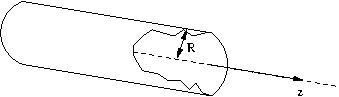
\includegraphics[width=0.5\linewidth]{TeX_files/chapter05-FlujoViscoco/Figures/tubo}
\end{center}

			
			
\begin{equation}
				u_{\theta}=u_{r}=0
\end{equation}
			
			
			Simetría cilíndrica $\rightarrow\dparc{}{\theta}=0$.
			
			Menospreciamos la gravedad y consideramos flujo estacionario.
			
			Ecuación de continuidad: 
			
\begin{equation}
				\dparc{u_{z}}{z}=0\,\Rightarrow\,u_{z}=u_{z}(r)
\end{equation}
			
	
	La ecuación de Navier-Stokes para $u_{z}$ en coordenadas cilíndricas
	es
	\[
	\begin{split}\underbrace{\dparc{u_{z}}{t}}_{\binom{=0}{\text{(estac.)}}}+\underbrace{u_{r}\dparc{u_{z}}{r}}_{\binom{=0}{u_{r}=0}}+\underbrace{u_{\theta}\frac{1}{r}\dparc{u_{z}}{\theta}}_{\binom{=0}{u_{\theta}=0}}+\underbrace{u_{z}\dparc{u_{z}}{z}}_{\binom{=0}{u_{z}=u_{z}(r)}}=\\
		-\frac{1}{\rho}\dparc{p}{z}+\frac{\mu}{\rho}\Bigl[\frac{1}{r}\dparc{}{r}\Bigl(r\dparc{u_{z}}{r}\Bigr)+\underbrace{\frac{1}{r^{2}}\dparcsec{u_{z}}{\theta}}_{\binom{=0}{u_{z}=u_{z}(r)}}+\underbrace{\dparcsec{u_{z}}{z}}_{\binom{=0}{u_{z}=u_{z}(r)}}\Bigr]
	\end{split}
	\]
	
	
\begin{equation}
		\Rightarrow\;\frac{\mu}{r}\deriv{}{r}\left(r\deriv{u_{z}}{r}\right)=\dparc{p}{z}
\end{equation}
	
	
	La ecuación de Navier-Stokes para $u_{r}$ da la condición $\dparc{p}{r}=0$,
	de forma que $p=p(z)$ 
	\[
	\frac{\mu}{r}\deriv{}{r}\left(r\deriv{u_{z}}{r}\right)=\deriv{p}{z}=\text{const}<0
	\]
	
	
	Integrando dos veces esta ecuación, obtenemos
	
	\[
	\deriv{}{r}\left(r\deriv{u_{z}}{r}\right)=\frac{1}{\mu}\deriv{p}{z}r\,\Rightarrow\,\,r\deriv{u_{z}}{r}=\frac{1}{2\mu}\deriv{p}{z}r^{2}+C_{1}
	\]
	
	\[
	\deriv{u_{z}}{r}=\frac{1}{2\mu}\deriv{p}{z}r+\frac{C_{1}}{r}\,\Rightarrow\,u_{z}=\frac{1}{4\mu}\deriv{p}{z}r^{2}+C_{1}\ln r+C_{2}
	\]
	
	Dado que $\ln0$ es una singularidad y en $r=0$ la velocidad del
	flujo ha de ser finita, se tiene que cumplir que $C_{1}=0$.
	
	La condición de contorno $u_{z}=0$ en $r=R$, lleva a 
	\[
	C_{2}=-\frac{1}{4\mu}\deriv{p}{z}R^{2}
	\]
	
	El flujo de Hagen-Poiseuille es, entonces, 
	
\begin{equation}
		\boxed{u_{z}=\left(-\deriv{p}{z}\right)\frac{1}{4\mu}\left(R^{2}-r^{2}\right)}
\end{equation}
	
	
	\subsection*{Actividad 4:}
		Calcular el caudal y el esfuerzo tangencial en las paredes de la
		tubería.

\section{Flujo entre dos cilindros rotatorios concéntricos}
	
	Consideramos el flujo entre dos cilindros concéntricos infinitamente
	largos, de forma que no hay flujo axial ($u_{z}=0,\dparc{}{z}=0$)
	ni efectos de final de tubo.
	
	Los radios de los cilindros en contacto con el fluido son $R_{1}$
	para el interior y $R_{2}$ para el exterior. El cilindro exterior
	está fijo, mientras que el interior rota con una velocidad $\Omega_{1}$.
	Hay simetria cilí ndrica, de forma que no hay variación de la velocidad
	con $\theta$.
	
	La ecuación de continuidad en coordenadas cilíndricas es 
	\[
	\frac{1}{r}\dparc{(ru_{r})}{r}+\underbrace{\frac{1}{r}\dparc{u_{\theta}}{\theta}}_{\binom{=0}{\dparc{}{\theta}=0}}=0\;\Rightarrow\;\frac{1}{r}\deriv{(ru_{r})}{r}=0\;\Rightarrow\;ru_{r}=\text{const.}
	\]
	
	
	Dado que $u_{r}=0$ en $R_{1}$ y en $R_{2}$, se deduce que $u_{r}=0$
	en todo el flujo, y la velocidad es siempre tangencial, $u_{\theta}=u_{\theta}(r)$.
	
	La ecuación de Navier-Stokes para $u_{\theta}$ es, considerando flujo
	estacionario y que no hay gravedad, 
	\[
	\bigl(\vec{u}\cdot\vec{\nabla}\bigr)u_{\theta}+\underbrace{\frac{1}{r}u_{r}u_{\theta}}_{\binom{=0}{u_{r}=0}}=-\underbrace{\frac{1}{r\rho}\dparc{p}{\theta}}_{\binom{=0}{\dparc{}{\theta}=0}}+\frac{\mu}{\rho}\bigl(\triangle u_{\theta}-\frac{u_{\theta}}{r^{2}}+\underbrace{\frac{2}{r^{2}}\dparc{u_{r}}{\theta}}_{\binom{=0}{\dparc{}{\theta}=0}}\bigr)
	\]
	
	La aceleración convectiva también se anula, 
	\[
	\bigl(\vec{u}\cdot\vec{\nabla}\bigr)u_{\theta}=\underbrace{u_{r}\dparc{u_{\theta}}{r}}_{\binom{=0}{u_{r}=0}}+\underbrace{\frac{1}{r}u_{\theta}\dparc{u_{\theta}}{\theta}}_{\binom{=0}{\dparc{}{\theta}=0}}+\underbrace{u_{z}\dparc{u_{\theta}}{z}}_{\binom{=0}{u_{z}=0}}=0
	\]
	y la ecuación se reduce a $\triangle u_{\theta}=\frac{u_{\theta}}{r^{2}}$.
	
	\[
	\triangle u_{\theta}=\frac{1}{r}\dparc{}{r}\left(r\dparc{u_{\theta}}{r}\right)+\underbrace{\frac{1}{r^{2}}\dparcsec{u_{\theta}}{\theta}}_{\binom{=0}{\dparc{}{\theta}=0}}+\underbrace{\dparcsec{u_{\theta}}{z}}_{\binom{=0}{\dparc{}{z}=0}}=\frac{1}{r}\deriv{}{r}\left(r\deriv{u_{\theta}}{r}\right)=\frac{u_{\theta}}{r^{2}}
	\]
	
	La solución general de esta ecuación diferencial ordinaria es 
	\[
	u_{\theta}=C_{1}r+\frac{C_{2}}{r}
	\]
	que, con las condiciones de contorno, {\small{}
		\[
		\left.\begin{array}{ll}
			r=R_{1}\rightarrow & u_{\theta}=\Omega_{1}R_{1}\,\rightarrow\,\Omega_{1}R_{1}=C_{1}R_{1}+\frac{C_{2}}{R_{1}}\\
			r=R_{2}\rightarrow & u_{\theta}=0\,\rightarrow\,0=C_{1}R_{2}+\frac{C_{2}}{R_{2}}
		\end{array}\right\} \Rightarrow\left\{ \begin{array}{l}
			C_{1}=-\dfrac{\Omega_{1}}{\frac{R_{2}^{2}}{R_{1}^{2}}-1}\\
			C_{2}=\dfrac{\Omega_{1}R_{2}^{2}}{\frac{R_{2}^{2}}{R_{1}^{2}}-1}
		\end{array}\right.
		\]
	} 
	\[
	\boxed{u_{\theta}=\frac{\Omega_{1}}{\Bigl(\frac{R_{2}^{2}}{R_{1}^{2}}-1\Bigr)}\Bigl(\frac{R_{2}^{2}}{r}-r\Bigr)}\quad R_{1}\leq r\leq R_{2}
	\]

	
	\subsection*{Actividad 5:}
		Demostrar que el esfuerzo tangencial en el caso de $u_{\theta}(r)$
		es 
		\[
		\tau_{\theta r}=-2\mu\frac{C_{2}}{r^{2}}
		\]

	
	\subsection*{Actividad 6:}
		Cilindro interior: $R_{1}=10\,\text{cm}$ . Exterior: $R_{2}=11\,\text{cm}$.
		Altura: $h=30\,\text{cm}$. Velocidad angular: $\Omega=1200\,\text{rpm}.$
		El fluido tiene una viscosidad $\mu=0.2\,\text{Pa s}$. Calcular el
		momento del rozamiento en el cilindro interior y comparar con el caso
		en que suponíamos una distribución lineal de velocidades.

	

\chapter[Análisis Dimensional]{Análisis Dimensional y Teoria de Modelos}

	
	En experimentos normalmente el número de variables que intervienen
	es muy grande. El análisis dimensional permite reducir el número de
	variables mediante el cálculo de \textcolor{red}{grupos adimensionales}.
	
	El análisis de los datos experimentales es así mucho más claro y sencillo.
	
	El ejemplo más típico es el de arrastre de un flujo sobre una esfera.
	Si diseñamos un experimento para estudiar éste arrastre en funcón
	de las variables físicas, debemos tener en cuenta las variaciones
	de 
	\begin{itemize}
		\item {el diámetro de la esfera, $d$} 
		\item {la velocidad del flujo, $v$} 
		\item {la densidad del fluido, $\rho$} 
		\item {la viscosidad del fluido, $\mu$} 
	\end{itemize}
	Ésto representan muchos experimentos.

	
	Sin embargo, el Análisis Dimensional permite demostrar que sólo hay
	que considerar dos variable o grupos adimensionales. Es usual usar
	los grupos 
	\[
	\frac{F_{D}}{\frac{1}{2}\rho v^{2}S}
	\]
	y 
	\[
	\frac{\rho vd}{\mu}
	\]
	
	Esto nos permite hacer experimentos variando únicamente la velocidad
	$v$, sin preocuparnos por la densidad, diámetro, viscosidad, \ldots{}
	Dos experimentos con la misma relación $\frac{\rho vd}{\mu}$ nos
	darán como resultado la misma relación $\frac{F_{D}}{\frac{1}{2}\rho v^{2}S}$.
	
	Ésto es útil para experimentar sobre modelos a escala de un diseño,
	sin fabricar el prototipo, que puede ser caro. El modelo ha de ser
	\textcolor{green}{geométricamente similar} al prototipo. Si la relación
	$\frac{\rho vd}{\mu}$ es también igual se dicen que el modelo y el
	prototipo son \textcolor{green}{dinámicamente similares}.

	
	\subsection*{Ejemplo:}
		Se mide la fuerza de arrastre que actúa sobre una esfera de  de diámetro
		en agua a  con una velocidad de  y se observa que es . ?`Cuál debería
		ser la velocidad para una esfera de  de diámetro en aire estándar
		a nivel del mar para qe los experimentos sean dinámicamente similares?
		?`Y cuál sería la fuerza medida?
		
		La densidad del agua es $\rho_{1}=1000\,\text{Kg}/\text{m}^{3}$,
		y la viscosidad es $\mu_{1}=10^{-3}\,\text{Pa}\cdot\text{s}$, de
		forma que 
		\[
		\frac{\rho_{1}v_{1}d_{1}}{\mu_{1}}=\frac{(1000\,\text{Kg}/\text{m}^{3})(2\,\text{m/s})(0.08\,\text{m})}{10^{-3}\,\text{Pa}\cdot\text{s}}=1.6\times10^{5}
		\]
		y 
		\[
		\frac{{F_{D}}_{1}}{\frac{1}{2}\rho_{1}v_{1}^{2}S_{1}}=\frac{5\,\text{N}}{0.5(1000\,\text{Kg}/\text{m}^{3})(2\,\text{m/s})^{2}\pi(0.04\,\text{m})^{2}}=0.497
		\]

		La densidad y la viscosidad del aire a $20\,^{\circ}C$ son, respectivamente,
		$\rho_{2}=1.2\,\text{Kg}/\text{m}^{3}$ y $\mu_{2}=1.8\times10^{-5}\,\text{Pa}\cdot\text{s}$,
		de forma que, si han de ser dinámicamente similares, 
		\[
		\frac{\rho_{2}v_{2}d_{2}}{\mu_{2}}=\frac{(1.2\,\text{Kg}/\text{m}^{3})v_{2}(1.5\,\text{m})}{1.8\times10^{-5}\,\text{Pa}\cdot\text{s}}=1.6\times10^{5}
		\]
		
		\[
		\Rightarrow v_{2}=1.6\,\text{m/s}
		\]
		y la fuerza medida será 
		\[
		\frac{{F_{D}}_{2}}{\frac{1}{2}\rho_{2}v_{2}^{2}S_{2}}=\frac{{F_{D}}_{2}}{0.5(1.2\,\text{Kg}/\text{m}^{3})(1.6\,\text{m/s})^{2}\pi(0.75\,\text{m})^{2}}=0.497
		\]
		
		\[
		\Rightarrow{F_{D}}_{2}=1.35\,\text{N}
		\]
	

\section{El Teorema $\Pi$ de Buckingham}

	
	Los productos adimensionales de variables físicas, como $\frac{F_{D}}{\frac{1}{2}\rho v^{2}S}$
	y $\frac{\rho vd}{\mu}$ reciben el nombre de \textcolor{green}{grupos
		adimensionales}, o \textcolor{green}{grupos $\Pi$}. Muchas veces
	reciben nombre propios. A $\frac{F_{D}}{\frac{1}{2}\rho v^{2}S}$
	se le denota como $C_{D}$, y es el coeficiente de arrastre. $\frac{\rho vd}{\mu}$
	es $\text{Re}$, el número de Reynolds.
	
	Veamos cómo se calculan de forma general estos grupos:
	
	La variables físicas vienen definidas en un conjunto de dimensiones
	básicas. Estas dimensiones suelen ser la masa ($M$), la longitud
	($L$) y el tiempo($T$). 
	
	{\footnotesize{}En problemas con variables termodinámicas podemos
		también tener la temperatura ($\Theta$), pero en general el número
		de dimensiones básicas será 3.}{\footnotesize\par}
	
	En las siguientes tablas se listan algunas variables físicas importantes,
	sus dimensiones y sus unidades en S.I.

	\bigskip

\renewcommand{\arraystretch}{1.3} % Para cambiar altura de filas en la tabla
\begin{tabular}{|c|c|c|c|}
	\hline 
	\textbf{Magnitud}  & \textbf{Símbolo}  & \textbf{Dimensiones}  & \textbf{Sistema Internacional} \tabularnewline
	\hline 
	\hline 
	longitud  & $l$  & $\text{L}$  & $\text{m}$ \tabularnewline
	\hline 
	tiempo  & $t$  & $\text{T}$  & $\text{s}$ \tabularnewline
	\hline 
	masa  & $m$  & $\text{M}$  & $\text{Kg}$ \tabularnewline
	\hline 
	fuerza  & $F$  & $\text{M}\,\text{L}\,\text{T}^{-2}$  & N \tabularnewline
	\hline 
	velocidad  & $v$  & $\text{L}\,\text{T}^{-1}$  & $\text{m}/\text{s}$ \tabularnewline
	\hline 
	aceleración  & $a$  & $\text{L}\,\text{T}^{-2}$  & $\text{m}/\text{s}^{2}$ \tabularnewline
	\hline 
	energía  & $E$  & $\text{M}\,\text{L}^{2}\,\text{T}^{-2}$  & $\text{J}$ \tabularnewline
	\hline 
	potencia  & $P$ (o $N$)  & $\text{M}\,\text{L}^{2}\,\text{T}^{-3}$  & $\text{W}$ \tabularnewline
	\hline 
	área  & $A$ (o $S$)  & $\text{L}^{2}$  & $\text{m}^{2}$\tabularnewline
	\hline 
	volumen  & $V$  & $\text{L}^{3}$  & $\text{m}^{3}$ \tabularnewline
	\hline 
	caudal  & $Q$  & $\text{L}^{3}\,\text{T}^{-1}$  & $\text{m}^{3}/\text{s}$ \tabularnewline
	\hline 
	flujo másico  & $\dot{m}$  & $\text{M}\,\text{T}^{-1}$  & $\text{Kg}/\text{s}$ \tabularnewline
	\hline 
	presión  & $p$  & $\text{M}\,\text{L}^{-1}\,\text{T}^{-2}$  & $\text{Pa}$ \tabularnewline
	\hline 
	gravedad  & $g$  & $\text{L}\,\text{T}^{-2}$  & $\text{m}/\text{s}^{2}$ \tabularnewline
	\hline 
	densidad  & $\rho$  & $\text{M}\,\text{L}^{-3}$  & $\text{Kg}/\text{m}^{3}$ \tabularnewline
	\hline 
	peso específico  & $\gamma$  & $\text{M}\,\text{L}^{-2}\,\text{T}^{-2}$  & $\text{N}/\text{m}^{3}$ \tabularnewline
	\hline 
	viscosidad dinámica  & $\mu$  & $\text{M}\,\text{L}^{-1}\,\text{T}^{-1}$  & $\text{Kg}/\text{m}\,\text{s}$ (o $\text{Pa}\,\text{s}$) \tabularnewline
	\hline 
	viscosidad cinemática  & $\nu$  & $\text{L}^{2}\,\text{T}^{-1}$  & $\text{m}^{2}/\text{s}$ \tabularnewline
	\hline 
	velocidad del sonido  & $c$  & $\text{L}\,\text{T}^{-1}$  & $\text{m}/\text{s}$ \tabularnewline
	\hline 
	tensión superficial  & $\sigma$  & $\text{M}\,\text{T}^{-2}$  & $\text{N}/\text{m}$ \tabularnewline
	\hline 
	módulo de compresibilidad  & $B$  & $\text{M}\,\text{L}^{-1}\,\text{T}^{-2}$  & $\text{Pa}$ \tabularnewline
	\hline 
	temperatura  & $T$  & $\Theta$  & K\tabularnewline
	\hline 
	conductividad térmica  & $k$  & $\text{M}\,\text{L}\,\text{T}^{-3}\,\Theta^{-1}$  & $\text{W}/\text{m}\,\text{K}$ \tabularnewline
	\hline 
	difusividad térmica  & $\alpha$  & $\text{L}^{2}\,\text{T}^{-1}$  & $\text{m}^{2}/\text{s}$ \tabularnewline
	\hline 
	difusividad  & $\mathcal{D}$  & $\text{L}^{2}\,\text{T}^{-1}$  & $\text{m}^{2}/\text{s}$ \tabularnewline
	\hline 
	capacidad calorífica  & $c_{p}$  & $\text{L}^{2}\,\text{T}^{-2}\,\Theta^{-1}$  & $\text{J}/\text{Kg}\,\text{K}$ \tabularnewline
	\hline 
\end{tabular}
\renewcommand{\arraystretch}{1}
	\bigskip

	El Teorema $\Pi$ de Buckingham garantiza que, \textcolor{blue}{dado
		un cierto fenómeno descrito por $n$ variables f\'{i}sicas, éste
		número puede reducirse a una relación de $k$ grupos adimensionales,
		donde $j=n-k$ es igual al número de variables que no pueden formar
		un $\Pi$ y siempre es igual o menor que el número de dimensiones
		que describen las variables.}
	
	Para formar los $\Pi$'s, seleccionamos $j$ variables independientes
	(en el sentido de que no pueden formar ellas solas un $\Pi$), y escribimos
	cada grupo adimensional añadiendo al producto general de potencias
	de estas variables cada una del resto de las variables, que puede
	estar elevada a una cierta potencia también. Cada una de estas combinaciones
	ha de ser adimensional. De esta condición se obtienen las potencias
	adecuadas de las variables.
	
	Parece un poco complicado, pero en realidad es muy simple y tan sólo
	hace falta un poco de práctica. Veamos un ejemplo.

	
	\subsection*{Ejemplo:}
		En el arrastre de la bola, sabemos que intervienen:
		
		- la fuerza de arrastre $F_{D}$, que es la variable dependiente,
		y que tiene unidades $N$, es decir, $MLT^{-2}$ 
		
		- el diámetro de la bola, $d$, con unidades $L$ 
		
		- la velocidad del flujo $v$, con $LT^{-1}$ 
		
		- la densidad del fluido $\rho$, con $ML^{-3}$ 
		
		- la viscosidad del fluido $\mu$, con $ML^{-1}T^{-1}$ 
		
		$j$ será como mucho 3, debido a que no tenemos la temperatura $\Theta$.
		Después de estudiar el sistema, vemos que $\rho$, $v$ y $d$ ser\'{i}a
		una buena selección, ya que no pueden formar un $\Pi$, y son bastante
		generales. Evidentemente, hay múltiples posibilidades correctas. Habrán
		entonces $5-3=2$ grupos adimensionales.
		
		El primer $\Pi$ lo fomariamos como 
		\[
		\Pi_{1}=\rho^{a}v^{b}d^{c}F_{D}
		\]
		
		Como ha de ser adimensional, las potencias $a$, $b$ y $c$ han
		de ser tales que se anulen las potencias de cada dimensión, es decir,
		\[
		(ML^{-3})^{a}(LT^{-1})^{b}(L)^{c}(MLT^{-2})=M^{0}L^{0}T^{0},
		\]
		y de aquí obtenemos tres ecuaciones para las potencias, 
		\begin{eqnarray*}
			\begin{cases}
				a+1 & =0\\
				-3a+b+c+1 & =0\\
				-b-2 & =0
			\end{cases}
		\end{eqnarray*}
		cuya solución es $(a=-1,b=-2,c=-2).$
		
		Por tanto, 
		\[
		\Pi_{1}=\rho^{-1}v^{-2}d^{-2}F_{D}=\frac{F_{D}}{\rho v^{2}d^{2}}.
		\]
		El coeficiente de arrastre $C_{D}$ es proporcional a este $\Pi$.

		El segundo $\Pi$ lo calculamos añadiendo la viscosidad al producto
		de las tres potencias de las variables, $\Pi_{2}=\rho^{a}v^{b}d^{c}\mu$,
		y la relación para obtener las potencias será 
		\[
		(ML^{-3})^{a}(LT^{-1})^{b}(L)^{c}(ML^{-1}T^{-1})=M^{0}L^{0}T^{0},
		\]
		que dará lugar al sistema 
		\begin{eqnarray*}
			\begin{cases}
				a+1 & =0\\
				-3a+b+c-1 & =0\\
				-b-1 & =0
			\end{cases}
		\end{eqnarray*}
		cuya solución es $a=b=c=-1.$
		
		Por tanto, 
		\[
		\Pi_{2}=\rho^{-1}v^{-1}d^{-1}\mu=\frac{\mu}{\rho vd}.
		\]
		El número de Reynolds es el inverso de este $\Pi$.

	
	\subsection*{Actividad 1:}
		La potencia consumida por una bomba es función del caudal $Q$, el
		tamaño de la bomba $D$ (es el diámetro externo del rodete, por ejemplo),
		la velocidad angular $\omega$, la densidad del fluido $\rho$ y su
		viscosidad $\mu$. Escribir como relación adimensional.
		
\section{Números adimensionales básicos}
	
	
	Existe una serie de grupos adimensionales clásicos en Mecánica de
	Fluidos. Algunos son más importantes que otros. En total existen cientos,
	pero en la siguiente tabla sólo vamos a indicar los más usados.
	
	
	
\renewcommand{\arraystretch}{1.3}	
	\begin{tabular}{|>{\raggedright}p{0.2\textwidth}|>{\centering}p{0.2\columnwidth}|>{\raggedright}p{0.5\textwidth}|}
		\hline 
		\textcolor{red}{número de Reynolds}{ } & {$\text{Re}=\frac{\rho uL}{\mu}$ } & {El más importante. Interviene siempre o casi siempre }\tabularnewline
		\hline 
		\textcolor{red}{número de Euler}{ } & {$\text{Eu}=\frac{\Delta p}{\rho u^{2}}$ } & {Si $\Delta p$ está relacionada con la presión de vapor, éste
			número es el }\textcolor{red}{coeficiente de cavitación}{ }\tabularnewline
		\hline 
		\textcolor{red}{número de Froude}{ } & {$\text{Fr}=\frac{u^{2}}{gL}$ } & {Flujos con superficie libre }\tabularnewline
		\hline 
		\textcolor{red}{número de Weber}{ } & {$\text{We}=\frac{\rho u^{2}L}{\sigma}$ } & {Flujos con superficie libre. $\sigma$ és la tensión superficial }\tabularnewline
		\hline 
		\textcolor{red}{número de Mach}{ } & {$\text{Ma}=\frac{u}{c}$ } & {Flujos compresibles. $c$ es la velocidad del sonido }\tabularnewline
		\hline 
		\textcolor{red}{número de Rossby}{ } & {$\text{Ro}=\frac{u}{\Omega L}$ } & {Flujos geof\'{i}sicos. $\Omega$ es la velocidad angular
			de la Tierra }\tabularnewline
		\hline 
		\textcolor{red}{coeficiente adiabático}{ } & {$\gamma=\frac{c_{p}}{c_{v}}$ } & { Flujos compresibles }\tabularnewline
		\hline 
		\textcolor{red}{número de Prandtl}{ } & {$\text{Pr}=\frac{\mu c_{p}}{k}$ } & { Convección térmica }\tabularnewline
		\hline 
		\textcolor{red}{número de Ecker}{ } & {$\text{Ec}=\frac{u^{2}}{c_{p}T_{0}}$ } & { Disipación térmica }\tabularnewline
		\hline 
		\textcolor{red}{número de Strouhal}{ } & {$\text{St}=\frac{\omega L}{u}$ } & { Flujos oscilatorios }\tabularnewline
		\hline 
		\textcolor{red}{rugosidad relativa y coeficiente de fricción}{ } & {$\frac{\epsilon}{D},\quad f=\frac{\Delta h_{r}}{\frac{L}{D}\frac{u^{2}}{2g}}$ } & { Flujos en tuber\'{i}as }\tabularnewline
		\hline 
		\textcolor{red}{coeficientes de presión} & {$C_{p}=\frac{p-p_{\infty}}{\frac{1}{2}\rho u^{2}}$ } & {Aerodinámica }\tabularnewline
		\hline 
		\textcolor{red}{coef. de sustentación}{ } & {$C_{L}=\frac{F_{L}}{\frac{1}{2}\rho u^{2}S}$ } & {Aerodinámica }\tabularnewline
		\hline 
		\textcolor{red}{coef. de arrastre}{ } & {$C_{D}=\frac{F_{D}}{\frac{1}{2}\rho u^{2}S}$ } & { Aerodinámica }\tabularnewline
		\hline 
	\end{tabular}
	\renewcommand{\arraystretch}{1}


\section{Adimensionalización de ecuaciones}

	
	
	En muchas ocasiones, es interesante escribir las ecuaciones básicas
	en forma adimensional. De esta forma se estan describiendo fenómenos
	con independencia de la magnitud de las escalas, y se puede apreciar
	mejor la relación entre términos.
	\subsection*{Ejemplo:}
		Como ejemplo, vamos a adimensionalizar la ecuación de Navier-Stokes
		para flujo incompresible (ver sesión ''Conservación de cantidad de
		movimiento II'') para el estudio típico de una esfera de diámetro
		$D$ en una corriente de un flujo con velocidad $V$ de un fluido
		de densidad $\rho$ y viscosidad $\mu$,
		\[
		\dparc{\vec{u}}{t}+\left(\vec{u}\cdot\vec{\nabla}\right)\vec{u}=\vec{g}-\frac{1}{\rho}\vec{\nabla}p+\frac{\mu}{\rho}\triangle\vec{u}
		\]
		

			En el problema que se está estudiando tenemos una velocidad de referencia
			$U$ y una longitud de referencia $D$. La velocidad y la posición
			pueden ser escritas de forma adimensional tomando estas magnitudes
			como referencia 
			\[
			\vec{u}^{\ast}=\frac{\vec{u}}{U}\quad;\quad\vec{r}^{\ast}=\frac{\vec{r}}{D}
			\]
			%
\begin{center}
	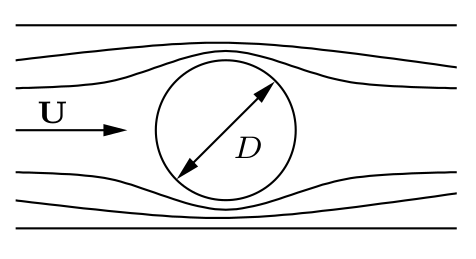
\includegraphics[width=0.5\linewidth]{TeX_files/chapter06-ADimensional/esfera}
\end{center}

		
		No olvidemos que estas relaciones son vectoriales, 
		\[
		\left\{ \begin{array}{l}
			u_{x}^{\ast}=\frac{u_{x}}{U}\\
			u_{y}^{\ast}=\frac{u_{y}}{U}\\
			u_{z}^{\ast}=\frac{u_{z}}{U}
		\end{array}\right.\quad;\quad\left\{ \begin{array}{l}
			x^{\ast}=\frac{x}{D}\\
			y^{\ast}=\frac{y}{D}\\
			z^{\ast}=\frac{z}{D}
		\end{array}\right.
		\]
		
		El tiempo adimensional se puede calcular usando como referencia $D/V$,
		que tiene dimensiones de tiempo, $t^{\ast}=\frac{t}{\frac{D}{U}}=\frac{tU}{D},$ 
		
		la gravedad adimensional es $\vec{g}^{\ast}=\frac{\vec{g}}{\frac{U^{2}}{D}}=\frac{D\vec{g}}{U^{2}},$ 
		
		y la presión adimensional es $p^{\ast}=\frac{p}{\rho U^{2}}.$
		
		Por otro lado, hay que tener en cuenta que las derivadas también son
		adimensionales, 
		\[
		\dparc{}{x}=\dparc{}{\left(Dx^{\ast}\right)}=\frac{1}{D}\dparc{}{x^{\ast}}\,\Rightarrow\,\left\{ \begin{array}{l}
			\vec{\nabla}=\frac{1}{D}\vec{\nabla}^{\ast}\\
			\\
			\triangle=\frac{1}{D^{2}}\triangle^{\ast}
		\end{array}\right.
		\]
		
		Adimensionalización de los términos de la Ecuación de Navier-Stokes:
		\begin{eqnarray*}
			\dparc{\vec{u}}{t} & = & \dparc{\left(U\vec{u}^{\ast}\right)}{\left(\frac{D}{U}t^{\ast}\right)}=\frac{U^{2}}{D}\dparc{\vec{u}^{\ast}}{t^{\ast}}\\
			\left(\vec{u}\cdot\vec{\nabla}\right)\vec{u} & = & \left(\left(U\vec{u}^{\ast}\right)\cdot\frac{1}{D}\vec{\nabla}^{\ast}\right)\left(U\vec{u}^{\ast}\right)=\frac{U^{2}}{D}\left(\vec{u}^{\ast}\cdot\vec{\nabla}^{\ast}\right)\vec{u}^{\ast}\\
			\vec{g} & = & \frac{U^{2}}{D}\vec{g}^{\ast}\\
			\frac{1}{\rho}\vec{\nabla}p & = & \frac{1}{\rho}\left(\frac{1}{D}\vec{\nabla}^{\ast}\right)\left(\rho U^{2}p^{\ast}\right)=\frac{U^{2}}{D}\vec{\nabla}^{\ast}p^{\ast}\\
			\frac{\mu}{\rho}\triangle\vec{u} & = & \frac{\mu}{\rho}\left(\frac{1}{D^{2}}\triangle^{\ast}\right)\left(U\vec{u}^{\ast}\right)=\frac{\mu U}{\rho D^{2}}\triangle^{\ast}\vec{u}^{\ast}
		\end{eqnarray*}
		
		Ecuación de Navier-Stokes adimensional: 
		\[
		\frac{U^{2}}{D}\dparc{\vec{u}^{\ast}}{t^{\ast}}+\frac{U^{2}}{D}\left(\vec{u}^{\ast}\cdot\vec{\nabla}^{\ast}\right)\vec{u}^{\ast}=\frac{U^{2}}{D}\vec{g}^{\ast}-\frac{U^{2}}{D}\vec{\nabla}^{\ast}p^{\ast}+\frac{\mu U}{\rho D^{2}}\triangle^{\ast}\vec{u}^{\ast}
		\]
		Dividiendo todos los términos por la aceleración de referencia $\frac{U^{2}}{D}$,
		\[
		\dparc{\vec{u}^{\ast}}{t^{\ast}}+\left(\vec{u}^{\ast}\cdot\vec{\nabla}^{\ast}\right)\vec{u}^{\ast}=\vec{g}^{\ast}-\vec{\nabla}^{\ast}p^{\ast}+\frac{\mu}{\rho DU}\triangle^{\ast}\vec{u}^{\ast}
		\]
		
		\[
		\dparc{\vec{u}^{\ast}}{t^{\ast}}+\left(\vec{u}^{\ast}\cdot\vec{\nabla}^{\ast}\right)\vec{u}^{\ast}=\vec{g}^{\ast}-\vec{\nabla}^{\ast}p^{\ast}+\frac{1}{\text{Re}}\triangle^{\ast}\vec{u}^{\ast}
		\]
		

	
	\subsection*{Actividad 1:}
		Consideremos la ecuación diferencial de conservación de la energía
		con las siguientes simplificaciones: 
		\begin{itemize}
			\item Sin fuentes puntuales de calor puntuales ($s=0$) 
			\item Flujo de calor únicamente debido a los gradientes de temperatura 
			\item Conductividad térmica uniforme 
			\item Flujo newtoniano 
		\end{itemize}
		
		Esta ecuación es 
		\[
		\dparc{\underline{u}}{t}+\left(\vec{u}\cdot\vec{\nabla}\right)\underline{u}=-\frac{1}{\rho}p\left(\vec{\nabla}\cdot\vec{u}\right)+\frac{1}{\rho}\Phi+\frac{1}{\rho}k\triangle T
		\]
		con 
		\[
		\Phi=\mu\sum_{ij}\left(\dparc{u_{i}}{x_{j}}+\dparc{u_{j}}{x_{i}}\right)^{2}
		\]
		
		Para simplificar más aún, supongamos que el fluido es incompresible,
		de forma que $\vec{\nabla}\cdot\vec{u}=0$, 
		\[
		\dparc{\underline{u}}{t}+\left(\vec{u}\cdot\vec{\nabla}\right)\underline{u}=\frac{1}{\rho}\Phi+\frac{1}{\rho}k\triangle T
		\]
		
		
		Para adimensionalizar esta expresión, conviene utilizar estos valores
		de referencia: 
		\begin{itemize}
			\item Temperatura: $T_{0}$ 
			\item Energía interna: $c_{p}T_{0}$ 
			\item Velocidad: $U$ 
			\item Tiempo: $\frac{k}{\rho c_{p}^{2}T_{0}}$ (comprobar que tiene dimensiones
			de tiempo) 
			\item Espacio: $\frac{kU}{\rho c_{p}^{2}T_{0}}$ 
		\end{itemize}
		
		Con estas referencias, adimensionalizar la ecuación de conservación
		de la energía y identificar los números adimensionales involucrados.
		

\section{Similitud}
	
	Antes de fabricar un prototipo y probarlo, se suelen realizar pruebas
	sobre un modelo a escala. Para que las pruebas sean válidas deben
	cumplirse ciertas condiciones: 
	\begin{itemize}
		\item \textcolor{red}{Similitud geométrica} : El prototipo y el modelo deben
		guardar las mismas proporciones espaciales en las tres dimensiones.
		Los ángulos relativos de la geometría deben ser iguales. 
		\item \textcolor{red}{Similitud cinemática} : Las velocidades deben guardar
		las mismas proporciones para el modelo y el prototipo. 
		\item \textcolor{red}{Similitud dinámica} : Las fuerzas (o bien las masas)
		en el prototipo y en el modelo deben guardar las mismas proporciones. 
	\end{itemize}

\subsection{Similitud cinemática}
	
	Es evidente que la similitud geométrica se ha de cumplir siempre.
	El factor de escala viene determinado por los recursos experimentales.
	
	
	En ocasiones la similitud cinemática está condicionada por la geométrica. 
	\subsection*{Ejemplo:}
		En un experimento se prueba un modelo a escala de un barco. El barco
		real (prototipo, posiblemente no fabricado aun) hace 70 metros de
		largo ($L_{p}=70\,\text{m}$). En el barco modelo la longitud es de
		70 centímetros ($L_{m}=0.7\,\text{m}$). El resto de dimensiones están
		a la misma escala 1:100.
		
		Queremos calcular la fricción que sufrirá el barco moviéndose a una
		velocidad de 50 nudos ($25.7\,\text{m/s}$). Dado que en un barco
		los efectos de la superficie libre son importantes, el número de Froude
		debe ser el mismo en el modelo. 

		El número de Froude es un número puramente cinemático (no interviene
		ninguna variable dinámica), y en el prototipo su valor es 
		\[
		\text{Fr}_{p}=\frac{u_{p}^{2}}{gL_{p}}=\frac{25.7^{2}}{9.8\times70}=0.96
		\]
		Para el modelo, el valor del número de Froude debe ser el mismo, 
		\[
		\text{Fr}_{m}=\frac{u_{m}^{2}}{gL_{m}}=\frac{u_{m}^{2}}{9.8\times0.7}=0.96,
		\]
		de forma que 
		\[
		u_{m}=\sqrt{0.96\times9.8\times0.7}=2.57\,\text{m/s}.
		\]
		En general, si $A$ es el factor de escala geométrica, el factor de
		velocidades será $\sqrt{A}$.

\subsection{Similitud dinámica}
	
	
	En función del tipo de fenómeno que estemos estudiando, algún número
	adimensional como Reynolds, Mach, Ecker o Euler deberá conservarse.
	Esto condiciona valores de velocidades, densidades, viscosidades,
	etc\ldots{}
	\subsection*{Ejemplo:}
		Siguiendo con el ejemplo anterior, además del número de Froude, el
		número de Reynolds deberá también ser igual. Esto implica 
		\[
		\text{Re}_{p}=\text{Re}_{m}
		\]
		
		\[
		\frac{\rho_{p}u_{p}L_{p}}{\mu_{p}}=\frac{\rho_{m}u_{m}L_{m}}{\mu_{m}}
		\]
		Para el agua, que es donde navegará el prototipo, $\rho_{p}=1000\,\text{Kg}/\text{m}^{3}$
		y $\mu_{p}=10^{-3}\,\text{N}/\text{m s}$, de forma que 
		\[
		\text{Re}_{p}=\frac{1000\times25.7\times70}{10^{-3}}=1.8\times10^{9}
		\]
		Esto da una condición para el fluido que debe usarse con el modelo,
		\[
		\frac{\rho_{m}}{\mu_{m}}=\frac{\text{Re}_{p}}{u_{m}L_{m}}=\frac{1.8\times10^{9}}{2.57\times0.7}=10^{9}\,\text{s}/\text{m}^{2}\,\Rightarrow\nu_{m}=10^{-9}\,\text{m}^{2}/\text{s}
		\]
		
	
	Quizás sería posible encontrar un fluido con esta característica,
	pero no sería barato (y probablemente sería bastante peligroso). El
	líquido más barato disponible es el agua y, desde luego, no tiene
	esta viscosidad cinemática. En muchas ocasiones se sacrifica la similitud
	dinámica en beneficio de la cinemática. Todo depende del experimento
	en concreto, y de la experiencia del ingeniero.
	

	
	\subsection*{Actividad 2:}
		La potencia $P$ que genera un aerogenerador depende del diámetro
		$D$, la densidad del aire $\rho$, la velocidad del viento $U$ y
		de la velocidad angular del aerogenerador $\Omega$.
		
		Escribir esta relación en forma adimensional.
		
		Se ha diseñado un aerogenerador que tendrá 5 metros de diámetro y
		funcionará a 2000 metros de altitud con vientos de 12 m/s. Antes de
		construirlo, fabricamos un modelo a escala, con 50 centímetros de
		diámetro y lo probamos en un tunel de viento a nivel de mar con una
		velocidad de 40 m/s y girando a 4800 rpm. La potencia que medimos
		es de 2700 w.
		
		Calcular la potencia que generará el prototipo y la velocidad a la
		que girará. 



\chapter[Turbulencia]{Breve introducción a la turbulencia}\label{Turbulencia}
\section{Promediado de Reynolds}

	
	\begin{itemize}
		\item Los flujos que encontramos en la industria, en el laboratorio, en
		la naturaleza son, normalmente, turbulentos.
		
		\begin{itemize}
			\item Excepciones: lubricación, microfluidos, \ldots{}
		\end{itemize}
		\item La \textcolor{blue}{transición a la turbulencia} ocurre para un determinado
		número de Reynolds, que no tiene porqué ser muy alto. Este \textcolor{red}{número
			de Reynolds crítico} depende del fenómeno en particular. 
		
		\begin{itemize}
			\item Por ejemplo, para flujo alrededor de una esfera, el flujo empieza
			a mostrarse turbulento para Re $\approx3\times10^{5}$. En el caso
			de flujos en el interior de una tubería, la transición puede empezar
			incluso para Re $\approx2000$, en función de las características.
		\end{itemize}
		\item Un flujo turbulento esta caracterizado por 
		
		\begin{itemize}
			\item la \textcolor{red}{imprevisibilidad}
			\item el \textcolor{red}{desorden} y 
			\item las rápidas \textcolor{red}{fluctuaciones}. 
		\end{itemize}
	\end{itemize}

	
	En teoría, debería ser posible su estudio con las ecuaciones de la
	dinámica ya estudiadas, pero, como se comentó anteriormente, estas
	ecuaciones son no-lineales, y tan solo se pueden resolver de forma
	analítica en muy pocos casos.
	
	Una solución es la resolución numérica. Pero esto implica un problema:
	
	Para poder resolver numéricamente las ecuaciones de Navier-Stokes,
	antes hay que discretizar el dominio de estudio, creando una malla.
	

\begin{center}
	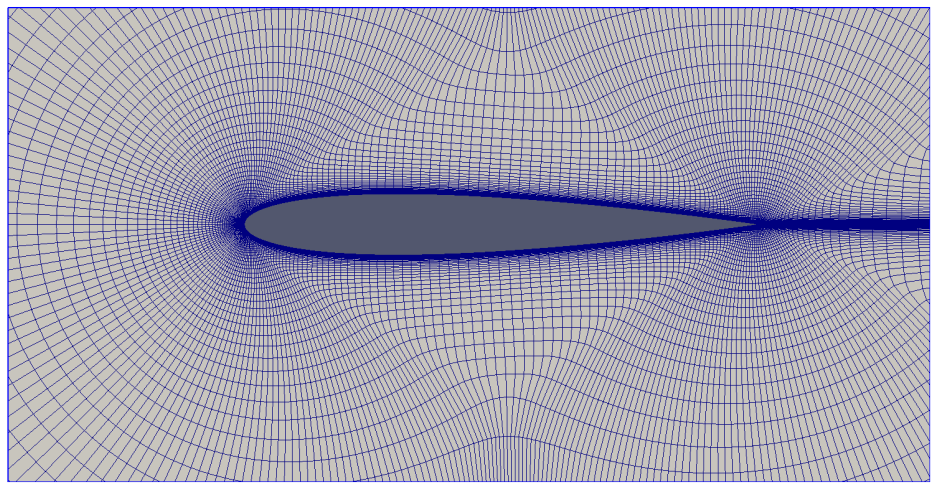
\includegraphics[width=0.7\linewidth]{TeX_files/chapter07-Turbulencia/airfoil}
\end{center}
	
	
	\begin{itemize}
		\item Las fluctuaciones espaciales de flujo turbulento son de varias escalas.
		Cuanto mayor es Re, más pequeñas pueden llegar a ser las fluctuaciones,
		y más fina tiene que ser la malla. 
		\item Pero, por otro lado, la resolución de la malla está limitada por la
		potencia del ordenador que se utilice. De este modo, el hardware nos
		limita Re.
		\item La potencia de los superordenadores crece de forma espectacular (ley
		de Moore), y el número de Reynolds de las simulaciones directas de
		las ecuaciones de Navier-Stokes va creciendo. Pero no todo el mundo
		tiene acceso a ellos.
		\item Cuando no es posible resolver de forma directa las ecuaciones de Navier-Stokes
		debido a que Re es muy grande y, por lo tanto, tendríamos que llegar
		a fluctuaciones de muy pequeño tamaño, se recurre a modelos de turbulencia,
		que nos predicen el comportamiento de las pequeñas escalas, de forma
		que sólo tenemos que preocuparnos de simular las grandes.
	\end{itemize}
	
	\textbf{Idea fundamental :}
		magnitud = magnitud media + fluctuaciones de magnitud.

	P.e., cualquier componente de la velocidad, o la presión : 
	\[
	u=\mean{u}+u'\,;\,p=\mean{p}+p'
	\]
	
	
	Consideremos que $L$ es una distacia típica macroscópica de nuestro
	problema (podría ser el tamaño medio de la discretización que nos
	podemos permitir con nuestro ordenador).
	
			
			\begin{center}
				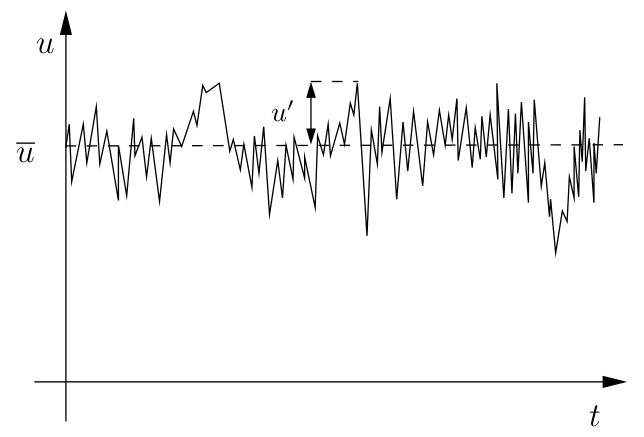
\includegraphics[width=0.7\linewidth]{TeX_files/chapter07-Turbulencia/noise}
			\end{center}
			

				\[
				\mean{u}=\frac{1}{T}\int_{0}^{T}u \dif t
				\]
				
				\[
				u'(x)=u-\mean{u}
				\]
				
				\[
	\mean{u'}=\mean{u-\mean{u}} =\mean{u}-\mean{\mean{u}}=\mean{u}-\mean{u}=0
				\]
			
			
			
				\[
				\mean{u'^{2}}=\frac{1}{T}\int_{0}^{T}u'^{2}\dif t\neq0
				\]
			

	
	La \textcolor{red}{intensidad de la turbulencia} se define como $I=\frac{\sqrt{\mean{u'^{2}}}}{\mean{u}}$
	
	Por regla general, $I$ en flujos típicos en Ingenieria es del orden
	del 10\% o 20\%.
	
	El producto de promedios no es necesariamente nulo. 
	\begin{align*}
		\mean{u'v'} & \neq0\\
		\mean{u'p'} & \neq0
	\end{align*}
	
	
	Descomponemos en promedios y fluctuaciones las tres componentes de
	la velocidad, 
	\begin{eqnarray*}
		u & = & \mean{u}+u'\\
		v & = & \mean{v}+v'\\
		w & = & \mean{w}+w'
	\end{eqnarray*}
	y escribimos la ecuación de continuidad para fluido incompresible
	\[
	\dparc{u}{x}+\dparc{v}{y}+\dparc{w}{z}=0
	\]
	usando esta descomposición 
	\[
	\dparc{}{x}\left(\mean{u}+u'\right)+\dparc{}{y}\left(\mean{v}+v'\right)+\dparc{}{z}\left(\mean{w}+w'\right)=0\;\Rightarrow\;\vec{\nabla}\cdot\vec{u}+\vec{\nabla}\cdot\vec{u}'=0
	\]
	
	
	Realizamos un promedio sobre esta expresión, 
	\[
	\mean{\vec{\nabla}\cdot\vec{u}}+\mean{\vec{\nabla}\cdot\vec{u}'}=\vec{\nabla}\cdot\mean{\vec{u}}+\underbrace{\vec{\nabla}\cdot\mean{\vec{u}'}}_{=0}=0.
	\]
	
	Esto indica que tanto la velocidad promedio como la fluctuación deben
	cumplir la condición de continuidad.
	
	\begin{eqnarray*}
		\vec{\nabla}\cdot\mean{\vec{u}} & = & 0\\
		\vec{\nabla}\cdot\vec{u}' & = & 0
	\end{eqnarray*}
	
	Escribimos también las ecuaciones de NS con esta descomposición y,
	a continuación, las promediamos. 
	
	Esto es lo que se conoce como \textbf{\textcolor{red}{Ecuaciones de
			Navier Stokes con Promediado de Reynolds}} (en inglés, RANS, Reynolds
	Averaged Navier Stokes). 

	
	Consideremos, por simplicidad, únicamente el caso de la componente
	$x$: 
	\[
	\rho\left[\dparc{u}{t}+u\dparc{u}{x}+v\dparc{u}{y}+v\dparc{u}{y}\right]=-\dparc{p}{x}+\dparc{\tau_{xx}}{x}+\dparc{\tau_{xy}}{y}+\dparc{\tau_{xz}}{z}
	\]
	donde el tensor de tensiones es sin traza, incluida en el término
	de las presiones.
	
	El primer término, después de promediar queda 
	\[
	\rho\dparc{\mean{u}}{t},
	\]
	igual que el término del gradiente de presión 
	\[
	\dparc{\mean{p}}{x}.
	\]
	
	
	En cambio, en la aceleración convectiva aparecen unos términos extras,
	\begin{eqnarray*}
		\mean{u\dparc{u}{x}}=\mean{u}\dparc{\mean{u}}{x}+\mean{u'\dparc{u'}{x}}=\mean{u}\dparc{\mean{u}}{x}+\dparc{}{x}{\mean{u'u'}}-\mean{u'\dparc{u'}{x}}\\
		\mean{v\dparc{u}{y}}=\mean{v}\dparc{\mean{u}}{y}+\mean{v'\dparc{u'}{y}}=\mean{v}\dparc{\mean{u}}{y}+\dparc{}{y}{\mean{v'u'}}-\mean{u'\dparc{v'}{y}}\\
		\mean{w\dparc{u}{z}}=\mean{w}\dparc{\mean{u}}{z}+\mean{w'\dparc{u'}{z}}=\mean{w}\dparc{\mean{u}}{z}+\dparc{}{z}{\mean{w'u'}}-\mean{u'\dparc{w'}{z}}
	\end{eqnarray*}
	
	\subsection*{Actividad 1:}
		Deducir las expresiones anteriores

\bigskip
	
	La ecuación de NS se puede escribir, después de reordenar términos,
	como
	
	\[
	\boxed{{\begin{split}\rho\left[\dparc{\mean{u}}{t}+\mean{u}\dparc{\mean{u}}{x}+\mean{v}\dparc{\mean{u}}{y}+\mean{w}\dparc{\mean{u}}{z}\right]=\\
				-\dparc{\mean{p}}{x}+\dparc{}{x}\bigl(\tau_{xx}-\rho\mean{u'u'}\bigr)+\dparc{}{y}\bigl(\tau_{xy}-\rho\mean{v'u'}\bigr)+\dparc{}{z}\bigl(\tau_{xz}-\rho\mean{w'u'}\bigr)
			\end{split}
	}}
	\]
	
	dado que 
	\[
	\mean{u'\dparc{u'}{x}}+\mean{u'\dparc{v'}{y}}+\mean{u'\dparc{w'}{z}}=\mean{u'\underbrace{\left(\dparc{u'}{x}+\dparc{v'}{y}+\dparc{w'}{z}\right)}_{=0}}=0
	\]
	

\section{Interpretación física del tensor de Reynolds}

	
	\begin{itemize}
		\item Las ecuaciones de Navier-Stokes para las velocidades y presión promedios
		son idénticas, excepto por la aparición de unos términos $-\rho\mean{u_{i}'u_{j}'}$,
		que se comportan como unos esfuerzos.
		\item Estos esfuerzo son los debidos a la cantidad de movimiento turbulenta
		transportada en el flujo, y son los responsables de la disipación
		de energia debida a las fluctuaciones.
		\item Estos términos $-\rho\mean{u_{i}'u_{j}'}$ forman el \textcolor{red}{tensor
			de esfuerzos turbulento}, o \textcolor{red}{tensor de Reynolds}. 
		\[
		\tau_{ij}^{t}=-\rho\mean{u_{i}'u_{j}'}
		\]
	\end{itemize}

	
	Nadie sabe a ciencia cierta cómo es este tensor, pero Prandtl propuso
	en 1930 el concepto de \textcolor{red}{viscosidad turbulenta}, $\mu_{t}$,
	como analogia con la viscosidad molecular y la ley de viscosidad de
	Newton, 
	\[
	\tau_{ij}^{t}\approx\mu_{t}\dparc{\mean{u_{i}}}{x_{j}}.
	\]
	Pero de nuevo nos encontramos con el problema del valor de $\mu_{t}$.
	Existen muchos modelos para calcularla, y el más sencillo fue propuesto
	también por Prandtl, y es conocido como el \textcolor{red}{modelo
		de la longitud de mezcla}, 
	\[
	\mu_{t}\approx\rho l^{2}\left|\dparc{\mean{u_{i}}}{x_{j}}\right|
	\]
	
	La longitud de mezcla $l$ es algo equivalente al recorrido libre
	medio de las partículas de un gas en mecánica estadística. Su valor
	dependerá del problema en concreto que queramos resolver.

\section{Ley de pared y capa límite turbulenta}

	
	El estudio de casos generales de flujos turbulentos es extremadamente
	complicado. Un caso relativamente sencillo es el estudio del flujo
	cerca de un sólido. Esta zona, en la que la velocidad del fluido tiende
	de forma suave a la del sólido es conocida como \textcolor{red}{capa
		límite}. Aquí tan sólo vamos a estudiarla de forma superficial, dejando
	este importante tema para más adelante.
	
\begin{center}
	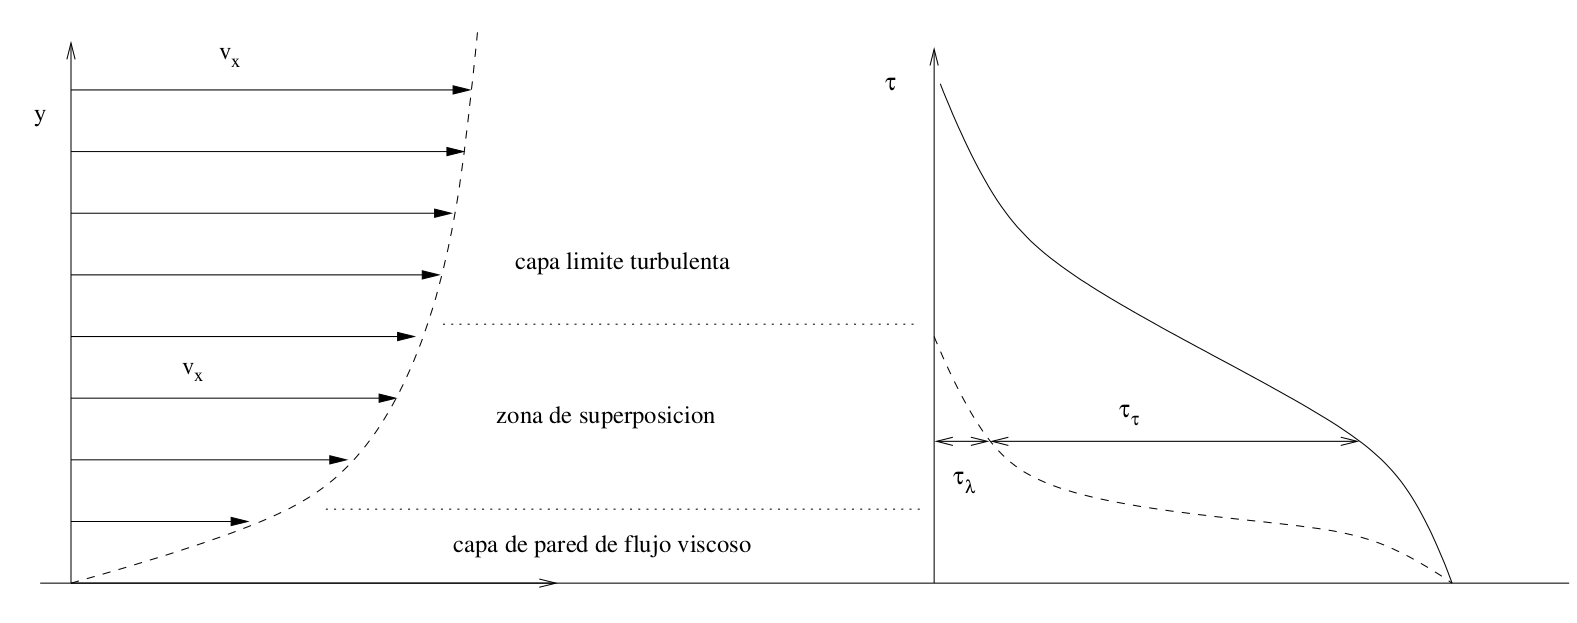
\includegraphics[width=0.7\linewidth]{TeX_files/chapter07-Turbulencia/pared}
\end{center}

	
	\begin{itemize}
		\item El espesor de la capa límite se define como la coordenada $y$ para
		la cual la velocidad alcanza el 99\% de la velocidad que tiene asintóticamente
		para $y\rightarrow\infty$. 
		\item $\tau_{p}$ es el esfuerzo tangencial en la pared.
		\item En la zona de la capa de pared, el flujo es laminar ya que la velocidad
		es pequeña y la viscosidad domina. 
		\item En esta zona, Prandtl dedujo en 1930 que el perfil de velocidad no
		puede depender del espesor de la capa límite, $\delta$. 
		\[
		u=f(\mu,\tau_{p},\rho,y)
		\]

		\item Por análisis dimensional, sabemos que esta ley estará definida por
		2 grupos adimensionales. 
		\[
		u^{+}=F(y^{+})
		\]
		donde 
		\[
		u^{+}=\frac{u}{u^{*}}\,;\,y^{+}=\frac{\rho u^{*}y}{\mu}\,;\,u^{*}=\sqrt{\frac{\tau_{p}}{\rho}}
		\]
		\item $u^{*}$ se denomina \textcolor{red}{velocidad de fricción} y, aunque
		tiene unidades de velocidad, en realidad no lo es.
		\item A la expresión $u^{+}=F(y^{+})$ se conoce como \textcolor{red}{ley
			de pared}, y llega hasta $y^{+}\approx10$. 
		
		\begin{itemize}
			\item Esta ley puede ser, por ejemplo, lineal, $u^{+}=y^{+}$.
		\end{itemize}
	\end{itemize}

	
	En cuanto a la capa externa turbulenta, el mismo Prandtl en 1933 dedujo
	que, dado que es turbulenta, la viscosidad no es importante, y la
	diferencia de la velocidad respecto de ${u}_{\infty}$ es función
	únicamente de $y$, del espesor de la capa límite, $\delta$, del
	esfuerzo tangencial en la pared, $\tau_{p}$, y de la densidad $\rho$,
	${u}_{\infty}-u=g(\delta,\tau_{p},\rho,y)$. De nuevo, el teorema
	$\Pi$ de Buckingham nos indica que esta ley viene dada por dos grupos
	adimensionales, 
	\[
	\frac{{u}_{\infty}-u}{u^{*}}=G\left(\frac{y}{\delta}\right).
	\]
	
	En la zona intermedia, sean cuales sean las formas de $F$ y $G$,
	éstas deben superponerse de forma suave. Se puede demostrar que ésto
	es sólo posible si la ley de velocidades en esta zona es logarítmica.
	\[
	\boxed{\frac{u}{u^{*}}=\frac{1}{\kappa}\ln\frac{\rho u^{*}y}{\mu}+B}
	\]
	con $\kappa\approx0.41$ y $B\approx5.0$. Ésta es la \textcolor{red}{ley
		logarítmica de superposición}, y se extiende hasta $y^{+}\approx1000$

	
	Del Kundu\cite{Kundu2012} (figura 12.18):
	
\begin{center}
	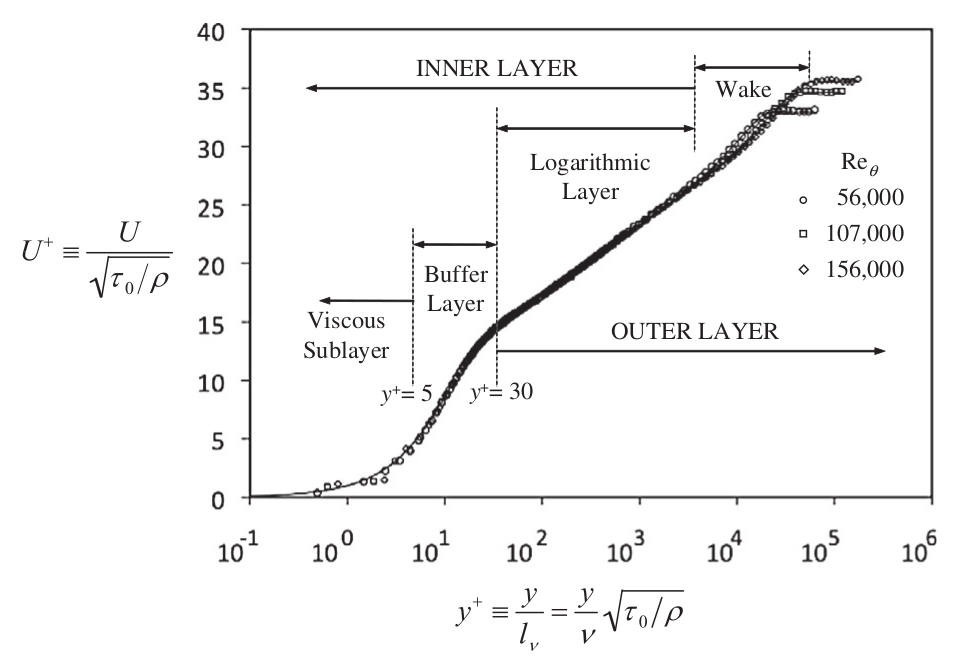
\includegraphics[width=0.7\linewidth]{TeX_files/chapter07-Turbulencia/LawOfWall}
\end{center}


	
	\subsection*{Actividad 2:}
		Si se considera el modelo de longitud de mezcla de Prandtl, cerca
		de la pared, con $l=\kappa y$, ($\kappa=0.41$ es la constante de
		Prandtl), se puede obtener la ley logarítmica de superposición, considerando
		que la ley de pared es lineal, $u^{+}=y^{+}$+ hasta $y^{+}=10$.
		
		Pista: considerar que $\tau_{t}\approx\tau_{p}$ independientemente
		de $y$.

	\subsection*{Actividad 3:}
		Para agua a 10 m/s de velocidad máxima, entre dos placas separadas
		1 cm, suponiendo que el flujo sigue la ley logarítmica, calcular $\tau_{p}$
		y el espesor de la subcapa laminar. Compara con el valor obtenido
		de $\tau_{p}$ si hubiesemos supuesto un flujo laminar viscoso, 
		\[
		u=\frac{4u_{max}}{h^{2}}y(h-y)
		\]


\chapter{Capa Límite}
	
	\begin{itemize}
		\item Por muy baja que sea la viscosidad de un fluido, en contacto con un
		sólido, la velocidad es la del sólido (generalmente, cero).
		\item Esto implica una zona de aumento progresivo de la velocidad desde
		0 hasta la velocidad del flujo en zonas no influenciadas por el sólido,
		$U_{\infty}$.
		\item Esta zona se denomina \textcolor{red}{\href{https://en.wikipedia.org/wiki/Boundary_layer}{capa límite}},
		y en ella se producen los efectos que realmente actúan sobre el sólido
		(arrastre, \ldots ).
		\item La capa límite puede ser laminar o turbulenta. El \textcolor{blue}{número
			de Reynolds local} que controla el régimen se define como 
		\[
		\text{Re}_{x}=\frac{\rho U_{\infty}x}{\mu}=\frac{U_{\infty}x}{\nu},
		\]
		donde $\rho$ es la densidad del fluido, $\mu$ es la viscosidad
		dinámica, $\nu$ es la viscosidad cinemática y $x$ es la distancia
		desde el punto en el que el flujo entra en contacto con el sólido.
		No hay un número concreto para la transición a capa límite turbulenta,
		pero está alrededor de $10^{6}$.
	\end{itemize}

	Consideremos, como ejemplo, el flujo sobre y bajo una placa lisa.

\begin{center}
	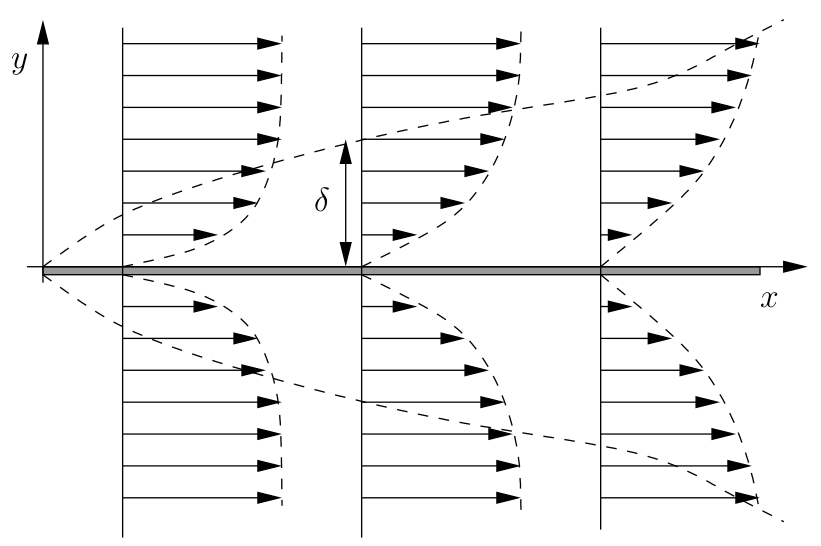
\includegraphics[width=0.7\linewidth]{TeX_files/chapter08-CapaLimite/capa1}
\end{center}
	
	
	El \textcolor{red}{espesor $\delta$} de la capa límite se define
	como la distancia de la placa para la cual la velocidad $v$ del flujo
	alcanza el 99\% de $U_{\infty}$.
	
	Pero se definen \href{https://en.wikipedia.org/wiki/Boundary_layer_thickness}{otros espesores}
	de la capa límite:
	
	\begin{itemize}
		\item \textcolor{red}{espesor de desplazamiento $\delta^{*}$}. Debido a
		la disminución de velocidad en la proximidad del sólido, se produce
		una pérdida de caudal. Se define $\delta^{*}$ como la distancia que
		habría que desplazar la placa con un fluido ideal sin viscosidad (no
		hay, por tanto, la condición de no deslizamiento) para que la pérdida
		de caudal fuese la misma.
		
		\begin{tabular}{cc}
			\begin{minipage}[c]{0.4\textwidth}%
\begin{center}
	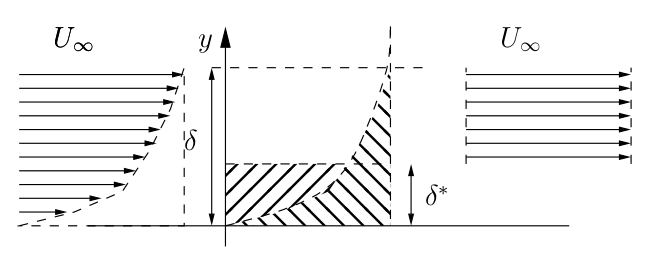
\includegraphics[width=\linewidth]{TeX_files/chapter08-CapaLimite/capa2}
\end{center}

			\end{minipage} & %
			\begin{minipage}[c]{0.5\textwidth}%
				
				\[
				U_{\infty}\delta^{*}b=\int_{0}^{\delta}\left(U_{\infty}-u\right)b\dif y
				\]
				
				
				\begin{equation}
					\Rightarrow\boxed{\delta^{*}=\int_{0}^{\delta}\left(1-\frac{u}{U_{\infty}}\right)\dif y}
				\end{equation}
				
				%
			\end{minipage}\tabularnewline
		\end{tabular}

		\item \textcolor{red}{espesor de cantidad de movimiento $\theta$}. Es la
		misma idea, pero con pérdida de cantidad de movimiento, en lugar de
		caudal. 
		\[
		U_{\infty}^{2}\theta=\int_{0}^{\delta}u\left(U_{\infty}-u\right)\dif y
		\]
		
		\begin{equation}
			\Rightarrow\boxed{\theta=\int_{0}^{\delta}\frac{u}{U_{\infty}}\left(1-\frac{u}{U_{\infty}}\right)\dif y}
		\end{equation}
		
		
	\end{itemize}
	Sobre cada pared de la placa se realiza un esfuerzo $\tau_{p}$, dado
	por 
	\[
	\tau_{p}=\mu\left.\dparc{u}{y}\right|_{y=0}
	\]
	
	El \textcolor{red}{coeficiente de esfuerzo superficial de pared} se
	define como 
	
\begin{equation}
		C_{f}=\frac{\tau_{p}}{\frac{1}{2}\rho U_{\infty}^{2}}
\end{equation}
	
	


\section{Capa límite laminar. Ecuación de Blasius}

	
	Considerando flujo estacionario, sin gradiente de presión, y que $\dparc{u}{y}\gg\dparc{u}{x}$,
	las ecuaciones de continuidad y NS son 
	\begin{eqnarray}
		u\dparc{u}{x}+v\dparc{u}{y}=\nu\dparcsec{u}{y}\\
		\dparc{u}{x}+\dparc{v}{y}=0
	\end{eqnarray}
	con las condiciones de contorno 
	\begin{eqnarray*}
		y=0\, & \rightarrow & \,u=0\\
		y=\infty\, & \rightarrow & \,\left\{ \begin{matrix}u=U_{\infty}\\
			\deriv{u}{y}=0
		\end{matrix}\right.
	\end{eqnarray*}
	
	Estas son conocidas como \textit{Ecuaciones de Prandtl}.
	

	
	Dado que el flujo es bidimensional, podemos usar la función de corriente
	$\psi$, 
	\begin{eqnarray*}
		u & = & \dparc{\psi}{y}\\
		v & = & -\dparc{\psi}{x}
	\end{eqnarray*}
	de esta forma, la ecuación de continuidad de cumple de forma automática.
	La ecuación de NS queda entonces como 
	\[
	\dparc{\psi}{y}\,\frac{\partial^{2}\psi}{\partial x\partial y}-\dparc{\psi}{x}\,\dparcsec{\psi}{y}=\nu\frac{\partial^{3}\psi}{\partial y^{3}}
	\]
	

	
	Para poder tratar esta ecuación se definen las variables adimensionales
	$f$ y $\eta$, con $\eta=\sqrt{\frac{U_{\infty}}{\nu x}}\,y$ y $f$
	es tal que $\deriv{f}{\eta}=\frac{u}{U_{\infty}}=\frac{1}{U_{\infty}}\dparc{\psi}{y}$.
	
	Al substituir en la ecuación de NS y tras varias operaciones algebraicas,
	obtenemos 
	\[
	\boxed{2\frac{\dif^{3}f}{\dif\eta^{3}}+f\derivsec{f}{\eta}=0}
	\]
	con las condiciones de contorno
	\[
	\begin{cases}
		\eta=0 & \rightarrow\,f=\deriv{f}{\eta}=0\\
		\eta=\infty & \rightarrow\,\deriv{f}{\eta}=1
	\end{cases}
	\]
	
	Esta es la conocida como \textcolor{red}{\href{https://en.wikipedia.org/wiki/Blasius_boundary_layer}{ecuación de Blasius}}
	(1908), y no se puede resolver analíticamente.

	
	La resolución numérica de esta ecuación indica que el espesor de la
	capa límite se alcanza para $\eta\approx5.0$. Es decir, 
	\[
	\delta\approx\frac{5.0}{\sqrt{\frac{U_{\infty}}{\nu x}}}=\frac{5.0x}{\sqrt{\text{Re}_{x}}}.
	\]
	Los otros espesores son, calculados mediante integración numérica,
	\begin{eqnarray*}
		\delta^{*} & = & 0.344\,\delta\\
		\theta & = & 0.133\,\delta
	\end{eqnarray*}
	
	El esfuerzo superficial sobre la placa viene dado por 
	\[
	\tau_{p}=\mu\left.\dparc{u}{y}\right|_{y=0}=\mu U_{\infty}\sqrt{\frac{U_{\infty}}{\nu x}}\,\left.\derivsec{f}{\eta}\right|_{\eta=0}
	\]
	

	
	De la misma solución numérica de la ecuación de Blasius, se comprueba
	que 
	\[
	\tau_{p}=0.332U_{\infty}\sqrt{\frac{\rho\mu U_{\infty}}{x}}=\frac{0.332\rho U_{\infty}^{2}}{\sqrt{\text{Re}_{x}}}
	\]
	y el coeficiente de esfuerzo superficial es 
	\[
	C_{f}=\frac{0.664}{\sqrt{\text{Re}_{x}}}
	\]
	
	Podemos calcular la fuerza de arrastre sobre una placa de longitud
	$L$ y amplitud $b$, 
	\[
	F_{D}=b\int_{0}^{L}\tau_{p}\dif x=0.332\rho U_{\infty}^{2}b\int_{0}^{L}\frac{1}{\sqrt{\text{Re}_{x}}}\dif x=0.664b\sqrt{\rho\mu LU_{\infty}^{3}}
	\]
	
	El \textcolor{red}{coeficiente de arrastre} sobre la placa será 
	\[
	C_{D}=\frac{F_{D}}{\frac{1}{2}\rho U_{\infty}^{2}bL}=\frac{1.328}{\sqrt{\text{Re}_{L}}}
	\]
	


\section[Ecuación de von Kármán]{Ecuación integral de von Kármán}

	
	\begin{tabular}{cc}
		\begin{minipage}[c]{0.4\textwidth}%
			\begin{center}
				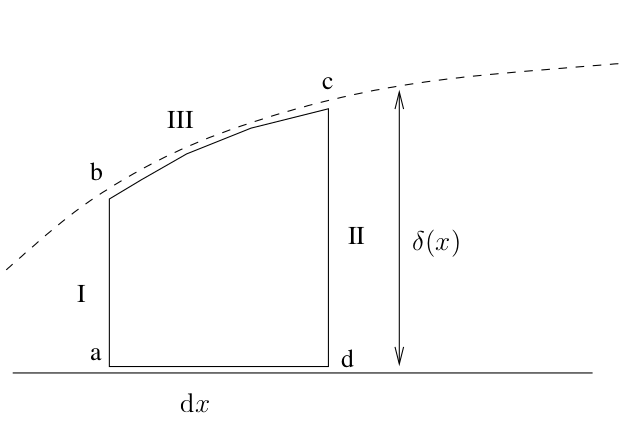
\includegraphics[width=1\linewidth]{TeX_files/chapter08-CapaLimite/vonKarman}
			\end{center}
			
		\end{minipage} & %
		\begin{minipage}[c]{0.5\textwidth}%
			Continuidad: 
			\begin{eqnarray*}
				\text{I :}Q_{ab} & = & -\int_{0}^{\delta}u(y)b\dif y\\
				\text{II :}Q_{cd} & = & -\left[Q_{ab}+\dparc{Q_{ab}}{x}\dif x\right]
			\end{eqnarray*}
			
			De aqui obtenemos el caudal que entra por III: 
			\[
			Q_{bc}=-b\dparc{}{x}\left[\int_{0}^{\delta}u(y)\dif y\right]\dif x
			\]
			%
		\end{minipage}\tabularnewline
	\end{tabular}

	
	Por otro lado, aplicamos la conservación de la cantidad de movimiento,
	\[
	F_{S}=\int_{SC}\rho u\vec{u}\cdot\dif\vec{S}
	\]
	
	\begin{eqnarray*}
		\text{I :} & -b\int_{0}^{\delta}\rho u(y)^{2}\dif y\\
		\text{II :} & b\left[\int_{0}^{\delta}\rho u(y)^{2}\dif y+\dparc{}{x}\left(\int_{0}^{\delta}\rho u(y)^{2}\dif y\right)\dif x\right]\\
		\text{III :} & -U_{\infty}b\dparc{}{x}\left[\int_{0}^{\delta}\rho u(y)\dif y\right]\dif x
	\end{eqnarray*}
	
	\[
	F_{S}=\left[-\deriv{p}{x}\,\dif x\delta-\tau_{p}\dif x\right]\,b
	\]
	
	\[
	-\deriv{p}{x}\delta-\tau_{p}=\dparc{}{x}\left(\int_{0}^{\delta}\rho u(y)^{2}\dif y\right)-U_{\infty}\dparc{}{x}\int_{0}^{\delta}\rho u(y)\dif y
	\]
	
	
	El gradiente de presiones se obtiene haciendo Bernoulli por la parte
	exterior de la capa límite, 
	\[
	\deriv{p}{x}=-\rho U_{\infty}\deriv{U_{\infty}}{x}
	\]
	y, operando, llegamos a 
	\[
	\boxed{\tau_{p}=\rho\deriv{}{x}\left(U_{\infty}^{2}\theta\right)+\rho\delta^{*}U_{\infty}\deriv{U_{\infty}}{x}}
	\]
	
	Esta es la \textcolor{red}{ecuación integral de cantidad de movimiento},
	y es una ecuación diferencial ordinaria, que nos permite calcular
	$\delta$ a partir de una suposición sobre la forma del perfil de
	velocidades.
	
	Si \textcolor{blue}{no hay gradiente de presiones}, $\deriv{U_{\infty}}{x}=0$,
	y la ecuación se reduce a
	
	\[
	\tau_{p}=\rho\deriv{}{x}\left(U_{\infty}^{2}\theta\right)
	\]
	
	
	\subsection*{Ejemplo:}
		Supongamos que el perfil de velocidades es de forma parabólica, 
		\[
		u=a+by+cy^{2}
		\]
		Las condiciones de contorno son, para $y=0$, $u=0$, y para $y=\delta$,
		$u=U_{\infty}$ y $\deriv{u}{y}=0$. Esto lleva a 
		\[
		\frac{u}{U_{\infty}}=2\zeta-\zeta^{2}
		\]
		con $\zeta=\frac{y}{\delta}$. El esfuerzo tangencial sobre la pared,
		según este perfil, es 
		\[
		\tau_{p}=\mu\left.\dparc{u}{y}\right|_{y=0}=2\frac{U_{\infty}\mu}{\delta}
		\]
		
		El espesor de cantidad de movimiento es {\small{}
			\[
			\theta=\int_{0}^{\delta}\frac{u(y)}{U_{\infty}}\left(1-\frac{u(y)}{U_{\infty}}\right)\dif y=\delta\int_{0}^{1}\frac{u(\zeta)}{U_{\infty}}\left(1-\frac{u(\zeta)}{U_{\infty}}\right)\dif\zeta=\frac{2}{15}\delta
			\]
		}Substituyendo en la ecuación integral de cantidad de movimiento sin
		gradiente de presiones, obtenemos 
		\[
		2\frac{U_{\infty}\mu}{\delta}=\frac{2}{15}\rho U_{\infty}^{2}\deriv{\delta}{x}
		\]
		que nos lleva a 
		\[
		\frac{1}{2}\delta^{2}=\frac{15\mu}{\rho U_{\infty}}x+C
		\]
		
		Dado que, para $x=0$, el inicio de la placa, la capa límite ha de
		tener un espesor nulo, $C=0$, de forma que 
		\[
		\delta=\sqrt{\frac{30\mu x}{\rho U_{\infty}}}=\frac{5.48x}{\sqrt{\text{Re}_{x}}}
		\]
		El esfuerzo tangencial en la pared es, para el perfil parabólico,
		\[
		\tau_{p}=\frac{0.365\rho U_{\infty}^{2}}{\sqrt{\text{Re}_{x}}},
		\]
		y los coeficientes de fricción y arrastre son 
		\[
		C_{f}=\frac{0.730}{\sqrt{\text{Re}_{x}}},\;C_{D}=\frac{1.460}{\sqrt{\text{Re}_{L}}}
		\]

	
	\subsection*{Actividad 1:}
		Repetir todos los pasos del ejemplo con un perfil sinusoidal, 
		\[
		\frac{u}{U_{\infty}}=\sin\left(\frac{\pi}{2}\zeta\right)
		\]

	
	
	\begin{tabular}{cc}
		\begin{minipage}[c]{0.75\textwidth}%
			Esta gráfica muestra la comparación entre el perfil de Blasius y los perficles parabólico y sinusiodal.
			\begin{center}
				\includegraphics[width=1\linewidth]{../../MFGA/Presentaciones/19-capalimite1/perfiles}
			\end{center}
			
			\begin{flushleft}
				\par\end{flushleft}%
		\end{minipage} & %
		\begin{minipage}[c]{0.25\textwidth}% 
			Estos son los valores numéricos para el perfil de Blasius.
				\begin{center}
					\begin{tabular}{|c|c|}
						\hline 
						$y/\delta$  & $u/U_{\infty}$ \tabularnewline
						\hline 
						\hline 
						0.0  & 0.0 \tabularnewline
						\hline 
						0.04  & 0.06641 \tabularnewline
						\hline 
						0.08  & 0.13277 \tabularnewline
						\hline 
						0.12  & 0.19894 \tabularnewline
						\hline 
						0.16  & 0.26471 \tabularnewline
						\hline 
						0.2  & 0.32979 \tabularnewline
						\hline 
						0.24  & 0.39378 \tabularnewline
						\hline 
						0.28  & 0.45627 \tabularnewline
						\hline 
						0.32  & 0.51676 \tabularnewline
						\hline 
						0.36  & 0.57477 \tabularnewline
						\hline 
						0.4  & 0.62977 \tabularnewline
						\hline 
						0.44  & 0.68132 \tabularnewline
						\hline 
						0.48  & 0.72899 \tabularnewline
						\hline 
						0.52  & 0.77246 \tabularnewline
						\hline 
						0.56  & 0.81152 \tabularnewline
						\hline 
						0.6  & 0.84605 \tabularnewline
						\hline 
						0.64  & 0.87609 \tabularnewline
						\hline 
						0.68  & 0.90177 \tabularnewline
						\hline 
						0.72  & 0.92333 \tabularnewline
						\hline 
						0.76  & 0.94112 \tabularnewline
						\hline 
						0.8  & 0.95552 \tabularnewline
						\hline 
						0.84  & 0.96696 \tabularnewline
						\hline 
						0.88  & 0.97587 \tabularnewline
						\hline 
						0.92  & 0.98269 \tabularnewline
						\hline 
						0.96  & 0.98779 \tabularnewline
						\hline 
						1  & 0.99155 \tabularnewline
						\hline 
					\end{tabular}
					\par\end{center}
		\end{minipage}\tabularnewline
	\end{tabular}

\section{Capa límite turbulenta}

	
	Partimos de la ecuación integral de cantidad de movimiento, que es
	válida tanto para flujo laminar como para turbulento. Consideremos
	que no hay gradiente de presiones. 
	\[
	\tau_{p}=\rho U_{\infty}^{2}\deriv{\theta}{x}
	\]
	
	Esta ecuación se puede escribir en términos adimensionales 
	\[
	C_{f}=2\deriv{\theta}{x}
	\]
	
	Como vimos en el tema de Turbulencia, el perfil turbulento de velocidades
	cerca de la pared se puede escribir como una ley logarítmica 
	\[
	\frac{u}{u^{*}}=\frac{1}{\kappa}\ln\frac{\rho u^{*}y}{\mu}+B\qquad;\qquad u^{*}=\sqrt{\frac{\tau_{p}}{\rho}}\quad\text{(velocidad de fricción)}
	\]
	

	
	Esta velocidad de fricción también se puede escribir como 
	\[
	u^{*}=\sqrt{\frac{1}{2}C_{f}U_{\infty}^{2}}=U_{\infty}\sqrt{\frac{C_{f}}{2}}
	\]
	
	Para $y=\delta$, la velocidad de fricción debe cumplir la ley logarítmica
	\[
	\frac{U_{\infty}}{u^{*}}=\frac{1}{\kappa}\ln\frac{\rho u^{*}\delta}{\mu}+B
	\]
	
	\[
	\sqrt{\frac{2}{C_{f}}}=\frac{1}{\kappa}\ln\left[\frac{\delta}{\nu}U_{\infty}\sqrt{\frac{C_{f}}{2}}\right]+B=\frac{1}{\kappa}\ln\left[\text{Re}_{\delta}\sqrt{\frac{C_{f}}{2}}\right]+B
	\]
	
	Debería ser posible resolver esta ecuación para obtener $C_{f}$ en
	función de $\text{Re}_{\delta}$, pero es imposible hacerlo de forma
	explícita, y usamos una forma aproximada 
	\[
	C_{f}=\frac{0.02}{\text{Re}_{\delta}^{1/6}}
	\]
	

	
	Introduciendo esta expresión en la ecuación integral de cantidad de
	movimiento, obtenemos 
	\[
	\frac{0.02}{\text{Re}_{\delta}^{1/6}}=2\deriv{\theta}{x}
	\]
	
	Con una expresión para el perfil de velocidades, podemos calcular
	\[
	\theta=\delta\int_{0}^{1}\frac{u(\zeta)}{U_{\infty}}\left(1-\frac{u(\zeta)}{U_{\infty}}\right)\dif\zeta
	\]
	con $\zeta=y/\delta$. 
	
	La expresión podria ser la ley logarítmica, pero complicaría de nuevo
	enormemente el cálculo, de forma que se usa una ley aproximada de
	potencia, $\frac{u(\zeta)}{U_{\infty}}=\zeta^{1/7},$ y se obtiene
	\[
	\theta=\delta\int_{0}^{1}\zeta^{1/7}\left(1-\zeta^{1/7}\right)\dif\zeta=\frac{7}{72}\delta.
	\]
	

	
	La ecuación integral de cantidad de movimiento queda entonces 
	\[
	\frac{0.02}{\text{Re}_{\delta}^{1/6}}=\frac{7}{36}\deriv{\delta}{x}
	\]
	
	\[
	\Rightarrow\,\text{Re}_{\delta}^{-1/6}=9.72\deriv{\delta}{x}=9.72\deriv{\text{Re}_{\delta}}{\text{Re}_{x}}
	\]
	
	\[
	\Rightarrow\text{Re}_{\delta}=0.16\text{Re}_{x}^{6/7}\,\Rightarrow\,\boxed{\delta=\frac{0.16x}{\text{Re}_{x}^{1/7}}}
	\]
	y de aqui es posible obtener también $C_{f}$, 
	\[
	C_{f}=0.02\text{Re}_{\delta}^{-1/6}=\frac{0.027}{\text{Re}_{x}^{1/7}}
	\]
	

	
	\subsection*{Ejemplo:}
		Consideremos agua con  sobre una placa plana rugosa, de forma que
		se induce una capa lí mite turbulenta desde el principio de la placa.
		Queremos calcular los espesores ,  y  y el esfuerzo superficial para
		. Compararemos con los resultados si la placa fuese completamente
		lisa.Calculamos en primer lugar el número de Reynolds local, $\text{Re}_{x}=\frac{U_{\infty}x}{\nu}=\frac{1\times1}{10^{-6}}=10^{6},$
		de forma que los espesores son 
		\begin{eqnarray*}
			\delta & = & \frac{0.16x}{\text{Re}_{x}^{1/7}}=\frac{0.16\times1}{10^{6/7}}=0.022\,\text{m}\\
			\delta^{*} & = & \delta\int_{0}^{1}\left(1-\zeta^{1/7}\right)\dif\zeta=\frac{1}{8}\delta=0.0028\,\text{m}\\
			\theta & = & \delta\int_{0}^{1}\zeta^{1/7}\left(1-\zeta^{1/7}\right)\dif\zeta=\frac{7}{72}\delta=0.0022\,\text{m}
		\end{eqnarray*}

		y el esfuerzo superficial es {\small{}
			\[
			\tau_{p}=C_{f}\frac{1}{2}\rho U_{\infty}^{2}=\frac{0.027}{\text{Re}_{x}^{1/7}}\frac{1}{2}\rho U_{\infty}^{2}=\frac{0.027}{10^{6/7}}\times\frac{1}{2}\times{1000}\times{1}=1.88\,\text{N}/\text{m}^{2}
			\]
		}
		
		Los cálculos de los espesores para una placa completamente lisa,
		y, por tanto, capa límite laminar, dan {\small{}
			\begin{eqnarray*}
				\delta & = & \frac{5.0x}{\sqrt{\text{Re}_{x}}}=\frac{5.0\times1}{\sqrt{10^{6}}}=0.005\,\text{m}=5\,\text{mm}\\
				\delta^{*} & = & 0.344\,\delta=0.0017\,\text{m}=1.7\,\text{mm}\\
				\theta & = & 0.133\,\delta=0.00066\,\text{m}=0.66\,\text{mm}
			\end{eqnarray*}
		} es decir, unas 4 veces más pequeños.
		
		El esfuerzo superficial es {\small{}
			\[
			\tau_{p}=C_{f}\frac{1}{2}\rho U_{\infty}^{2}=\frac{0.664}{\sqrt{\text{Re}_{x}}}\frac{1}{2}\rho U_{\infty}^{2}=\frac{0.664}{\sqrt{10^{6}}}\frac{1}{2}\times1000\times1=0.332\,\text{N}/\text{m}^{2},
			\]
		} unas 6 veces más pequeño que en el caso de placa rugosa.

		Supongamos que la placa hace un metro de ancho. La fuerza que hace
		el flujo de agua sobre una cara, hasta $L=1\,\text{m}$, es 
			\[
			F_{D}=\int_{S}\tau_{p}\dif S=b\int_{0}^{L}C_{f}\frac{1}{2}\rho U_{\infty}^{2}\dif x=b\frac{1}{2}\rho U_{\infty}^{2}\int_{0}^{L}C_{f}\dif x=C_{D}\frac{1}{2}\rho U_{\infty}^{2}bL
			\]
		
		
		En el caso turbulento,
			\[
			F_{D}=b\frac{1}{2}\rho U_{\infty}^{2}\int_{0}^{L}\frac{0.027}{\re_{x}^{1/7}}\dif x=\frac{1}{2}\rho U_{\infty}^{2}bL\frac{0.031}{\re_{L}^{1/7}}=\frac{1}{2}\times1000\times1\times1\times\frac{0.031}{{10^{6}}^{1/7}}=2.15\,\text{N}
			\]
		
		
		En el caso laminar,
			\[
			F_{D}=b\frac{1}{2}\rho U_{\infty}^{2}\int_{0}^{L}\frac{0.664}{\re_{x}^{1/2}}\dif x=\frac{1}{2}\rho U_{\infty}^{2}bL\frac{1.328}{\re_{L}^{1/2}}=\frac{1}{2}\times1000\times1\times1\times\frac{1.328}{{10^{6}}^{1/2}}=0.664\,\text{N}
			\]
		

\section{Capa límite con gradiente de presiones. Separación de flujo}

	
	¿ Qué ocurre cuando hay gradiente de presiones, o, lo que es lo mismo,
	$\deriv{U_{\infty}}{x}\neq0$ ?
	\begin{itemize}
		\item Si {\small{}
			\[
			\deriv{U_{\infty}}{x}>0\,\Rightarrow\,\deriv{p}{x}<0
			\]
		} se dice que tenemos un \textcolor{red}{gradiente de presiones favorable},
		y no ocurre nada especial. Solo que la ecuación integral de cantidad
		de movimiento es más complicada.
		\item Pero si {\small{}
			\[
			\deriv{U_{\infty}}{x}<0\,\Rightarrow\,\deriv{p}{x}>0
			\]
		} hay un \textcolor{red}{gradiente de presiones adverso} y es posible
		que ocurra una \textcolor{red}{\href{https://en.wikipedia.org/wiki/Flow_separation}{separación de flujo}}.
	\end{itemize}
	Ésto último ocurre cuando la capa lí mite crece tanto que no sólo
	el flujo en la pared es nulo, sino también su derivada {\small{}
		\[
		\left.\deriv{u}{y}\right|_{y=0}=0\,\Rightarrow\,\tau_{p}=0.
		\]
	}{\small\par}

	
\begin{center}
	\includegraphics[width=0.7\linewidth]{TeX_files/chapter08-CapaLimite/sepa}
\end{center}


	
	Recordemos que las expresiones para $C_{f}=\frac{\tau_{p}}{\frac{1}{2}\rho U_{\infty}^{2}}$
	son 
	\[
	C_{f}=\frac{\text{cte}}{\sqrt{\re_{x}}}\qquad\text{para flujo laminar}
	\]
	\[
	C_{f}=\frac{\text{cte}}{\re_{x}^{1/7}}\qquad\text{para flujo turbulento}
	\]
	lo cual implica que $\tau_{p}$ se anula únicamente para $\re_{x}\rightarrow\infty$.
	Sin embargo, estas expresiones fueron deducidas para el caso de gradiente
	de presiones nulo.
	
	La ecuación integral de cantidad de movimiento es 
	\[
	\tau_{p}=\rho\deriv{}{x}\left(U_{\infty}^{2}\theta\right)+\rho\delta^{*}U_{\infty}\deriv{U_{\infty}}{x}
	\]
	
	Desarrollándola y con la definición de $C_{f}$ podemos deducir 
	\[
	\frac{C_{f}}{2}=\deriv{\theta}{x}+(H+2)\frac{\theta}{U_{\infty}}\deriv{U_{\infty}}{x}\quad\text{; con}\,H=\frac{\delta^{*}}{\theta}\quad\textbf{factor de forma}
	\]
	
	
	Si calculamos $U_{\infty}(x)$, podemos integrar esta ecuación si
	conocemos $H(\theta)$ y $C_{f}(\theta)$ para encontrar el punto
	$x$ en el que ocurre la separación de flujo ($C_{f}=0$).\medskip{}
	


			Para flujo turbulento el cálculo es demasiado complicado y se deja
			fuera de este curso. Pero es importante notar que el hecho de que
			en la capa límite turbulenta $\theta$ sea mucho menor (en relación
			a $\delta$) que en la laminar hace que separarla de la superficie
			sólida sea más dificil. %

Esta gráfica muestra la comparación, para el mismo espesor, del perfil laminar (Blasius) y turbulento.

\begin{center}
	\includegraphics[width=0.7\linewidth]{../../MFGA/Presentaciones/20-capalimite2/perfiles}
\end{center}


\subsection{El método de Thwaites}
	
	Para capa límite laminar, en 1949 Thwaites encontró de forma experimental
	la relación 
	\[
	S(\lambda)=(\lambda+0.09)^{(0.62)},
	\]
	donde $S=\frac{\tau_{p}\theta}{\mu U_{\infty}}=\frac{1}{2}C_{f}\re_{\theta}$
	es un esfuerzo superficial adimensional, y $\lambda=\frac{\theta^{2}}{\nu}\deriv{U_{\infty}}{x}$
	es un espesor de cantidad de movimiento adimensional. Es necesario
	conocer el valor de $\theta$, que se puede calcular con la expresión
	también de Thwaites 
	\[
	\theta^{2}(x)=\theta_{0}^{2}\left(\frac{U_{0}}{U_{\infty}(x)}\right)^{6}+\frac{0.45\nu}{U_{\infty}^{6}(x)}\int_{0}^{x}U_{\infty}^{5}(x)\dif x
	\]
	
	Con esta expresión es posible calcular $\tau_{p}$ con gradiente de
	presiones y el punto $x$ en el que se produce la separación ($\lambda=-0.09$)
	con un error relativamente pequeño ($\pm10\%)$ respecto a la resolución
	numérica de las ecuaciones de capa límite.

	
	\subsection*{Ejemplo:}
		Consideremos una ley lineal de velocidad 
		\[
		U_{\infty}=U_{0}\left(1-\frac{x}{L}\right).
		\]
		
		Dado que la velocidad $U_{\infty}$ decrece con $x$, la presión crece,
		y tendremos un gradiente de presiones adverso. Si nos aseguramos de
		que en todo momento el flujo es laminar, podemos usar el método de
		Thwaites para calcular el punto de separación del flujo.
		
		Suponiendo que $\theta_{0}=0$, el espesor de cantidad de movimiento
		de la capa lí mite es {\footnotesize{}
			\[
			\theta^{2}(x)=\frac{0.45\nu}{U_{\infty}^{6}(x)}\int_{0}^{x}U_{\infty}^{5}(x)\dif x=\frac{0.45\nu}{U_{0}^{6}}\left(1-\frac{x}{L}\right)^{-6}\int_{0}^{x}U_{0}^{5}\left(1-\frac{x}{L}\right)^{5}\dif x
			\]
		} 
		\[
		\theta^{2}(x)=0.075\frac{\nu L}{U_{0}}\left[\left(1-\frac{x}{L}\right)^{-6}-1\right]
		\]
		
		y $\lambda$ es entonces 
		\[
		\lambda=\frac{\theta^{2}}{\nu}\deriv{U_{\infty}}{x}=-\frac{\theta^{2}U_{0}}{\nu L}=-0.075\left[\left(1-\frac{x}{L}\right)^{-6}-1\right]
		\]
		
		La separación del flujo se da para $\lambda_{sep}=-0.09$, es decir,
		\[
		\lambda_{sep}=-0.09=-0.075\left[\left(1-\frac{x_{sep}}{L}\right)^{-6}-1\right]
		\]
		
		\[
		\Rightarrow\,\frac{x_{sep}}{L}=0.123
		\]
		
		La solución exacta obtenida mediante simulación numérica es $x_{sep}=0.120L$.

	
	Para calcular $C_{f}$ en cualquier punto $\frac{x}{L}$ \textbf{antes}
	de la separación utilizamos 
	\[
	S=\frac{\tau_{p}\theta}{\mu U_{\infty}}=\frac{1}{2}C_{f}\re_{\theta}=(\lambda+0.09)^{0.62}
	\]
	
	En el caso del ejemplo anterior:
	
	\[
	\frac{1}{2}C_{f}\re_{\theta}=\left\{ -0.075\left[\left(1-\frac{x}{L}\right)^{-6}-1\right]+0.09\right\} ^{0.62}
	\]
	
	\[
	C_{f}\re_{\theta}=\left\{ 0.165-0.229\left(1-\frac{x}{L}\right)^{-6}\right\} ^{0.62}
	\]
	
	
	Para poder calcular $\re_{\theta}=\frac{U_{0}\theta}{\nu}$, usamos
	\[
	\theta^{2}(x)=0.075\frac{\nu L}{U_{0}}\left[\left(1-\frac{x}{L}\right)^{-6}-1\right]
	\]
	{\footnotesize{}
		\[
		\frac{U_{0}^{2}\theta^{2}(x)}{\nu^{2}}=\re_{\theta}^{2}=0.075\frac{U_{0}L}{\nu}\left[\left(1-\frac{x}{L}\right)^{-6}-1\right]=0.075\re_{L}\left[\left(1-\frac{x}{L}\right)^{-6}-1\right]
		\]
	} 
	\[
	\re_{\theta}=0.274\sqrt{\re_{L}}\left[\left(1-\frac{x}{L}\right)^{-6}-1\right]^{\frac{1}{2}}
	\]
	
	Para poder calcular $\re_{\theta}$ y, por lo tanto, $C_{f}$, se
	debe conocer $\re_{L}$. 
	\subsection*{Actividad:}
		Repetir los cálculos del ejemplo con 
		\[
		U_{\infty}=U_{0}\left(1-\frac{x^{2}}{L^{2}}\right)
		\]
		
		Cálculos precisos dan como punto de separación $\frac{x}{L}=0.271$. 

\chapter[Flujo Ideal y Externo]{Flujo Ideal y Externo}
\section{Ecuación de Euler}

	
	Consideremos un flujo no viscoso ($\mu=0$). La ecuación de Navier-Stokes
	queda entonces como 
	
\begin{equation}
		\Deriv{\vec{u}}{t}=\vec{g}-\frac{1}{\rho}\vec{\nabla}p
\end{equation}
	
	
\begin{equation}
		\dparc{\vec{u}}{t}+\convec\vec{u}=\vec{g}-\frac{1}{\rho}\vec{\nabla}p
\end{equation}
	
	
	La aceleración convectiva se puede escribir en términos da la vorticidad,
	que no es más que el rotacional de la velocidad, $\vec{\omega}=\rot\vec{u}$
	
\begin{equation}
		\convec\vec{u}=\vec{\nabla}\left(\frac{1}{2}u^{2}\right)+\vec{\omega}\times\vec{u}
\end{equation}
	
	
	
	Podemos entonces escribir 
	
\begin{equation}
		\dparc{\vec{u}}{t}+\vec{\nabla}\left(\frac{1}{2}u^{2}\right)+\vec{\omega}\times\vec{u}+\frac{1}{\rho}\vec{\nabla}p-\vec{g}=0
\end{equation}
	
	e integrarlo sobre un cierto camino 
	
\begin{equation}
		\int_{A}^{B}\left[\dparc{\vec{u}}{t}+\vec{\nabla}\left(\frac{1}{2}u^{2}\right)+\vec{\omega}\times\vec{u}+\frac{1}{\rho}\vec{\nabla}p-\vec{g}\right]\cdot\dif\vec{r}=0
\end{equation}
	
	
	Si, por simplicidad, consideramos que el flujo es estacionario, esta
	integral puede ser realizada siempre y cuando $\left(\vec{\omega}\times\vec{u}\right)\cdot\dif\vec{r}=0$.
	Esto ocurre, por ejemplo, si $\vec{u}\cdot\dif\vec{r}=0$. Es decir,
	si el camino es una \textbf{\textcolor{blue}{línea de corriente}}.

	
	En este caso, 
	\[
	\int_{A}^{B}\left[\vec{\nabla}\left(\frac{1}{2}u^{2}\right)+\frac{1}{\rho}\vec{\nabla}p-\vec{g}\right]\cdot\dif\vec{r}=0
	\]
	\[
	\Rightarrow\frac{1}{2}\left(u_{B}^{2}-u_{A}^{2}\right)+g(z_{B}-z_{A})+\int_{A}^{B}\frac{\dif p}{\rho}=0\textrm{ con }\vec{g}=-g\vec{k}
	\]
	
	Esta relación es la conocida \textcolor{blue}{Ecuación de Bernoulli},
	y es válida a lo largo de una línea de corriente. Pero si el flujo
	es irrotacional, es decir, es tal que 
	\[
	\rot\vec{u}=0
	\]
	en todo el dominio, entonces la ecuación de Bernoulli se cumple entre
	dos puntos cualesquiera.

	
	En este caso se cumple que la velocidad, como todo campo vectorial
	conservativo, se puede escribir como gradiente de una función $\phi$
	\[
	\vec{u}=\vec{\nabla}\phi
	\]
	que recibe el nombre de \textbf{\textcolor{red}{potencial de velocidad}}
	y este tipo de flujo se conoce como \textbf{\textcolor{red}{flujo
			potencial}}.
	
	El potencial de velocidad es una función escalar del tiempo y el espacio,
	$\phi(t,x,y,z)$ y se puede definir para cualquier campo de velocidades
	que sea irrotacional.
	
	Las líneas del espacio definidas por $\phi=\text{cte}$ son las \textcolor{blue}{líneas
		de potencial} del flujo.
	
	Para un flujo potencial la ecuación de continuidad se reduce a una
	\textbf{\textcolor{red}{ecuación de Laplace}} 
	\[
	\vec{\nabla}\cdot\vec{u}=0\enskip\Rightarrow\enskip\vec{\nabla}\left(\vec{\nabla}\phi\right)=\nabla^{2}\phi=0\;;\;\dparcsec{\phi}{x}+\dparcsec{\phi}{y}+\dparcsec{\phi}{z}=0
	\]
	

\section{Función de corriente}

	
	Recordemos que, para \textcolor{blue}{un flujo bidimensional}, la
	función de corriente se define como una función $\psi$ tal que $u=\dparc{\psi}{y},v=-\dparc{\psi}{x}$
	de forma que 
	\[
	\dif\psi=\dparc{\psi}{x}\dif x+\dparc{\psi}{y}\dif y=-v\dif x+u\dif y
	\]
	Si $\dif\psi=0$, entonces 
	\[
	\deriv{y}{x}=\frac{v}{u}\enskip\Rightarrow\enskip\psi=\text{cte define las lineas de corriente}
	\]
	Si el flujo es irrotacional 
	\[
	\left(\rot\vec{u}\right)_{z}=\dparc{v}{x}-\dparc{u}{y}=0\enskip\Rightarrow\enskip-\dparcsec{\psi}{x}-\dparcsec{\psi}{y}=0\enskip\Rightarrow\enskip\nabla^{2}\psi=0
	\]
	La función de corriente también cumple la equación de Laplace.

	
	En muchas ocasiones es conveniente (o imprescindible) trabajar en
	coordenadas polares. En estas coordenadas, las relaciones entre la
	velocidad, la función de corriente y el potencial de flujo son 
	\begin{eqnarray}
		u_{r} & = & \dparc{\phi}{r}=\frac{1}{r}\dparc{\psi}{\theta}\\
		u_{\theta} & = & \frac{1}{r}\dparc{\phi}{\theta}=-\dparc{\psi}{r}
	\end{eqnarray}
	y las ecuaciones de Laplace son 
	\begin{eqnarray}
		\frac{1}{r}\dparc{}{r}\left(r\dparc{\psi}{r}\right)+\frac{1}{r^{2}}\dparcsec{\psi}{\theta} & = & 0\\
		\frac{1}{r}\dparc{}{r}\left(r\dparc{\phi}{r}\right)+\frac{1}{r^{2}}\dparcsec{\phi}{\theta} & = & 0
	\end{eqnarray}
	


\section{La ecuación de vorticidad}

	
	Si volvemos a considerar la viscosidad, la ecuación de Navier-Stokes,
	se puede expresar como 
	
\begin{equation}
		\dparc{\vec{u}}{t}+\vec{\nabla}\left(\frac{1}{2}u^{2}\right)+\vec{\omega}\times\vec{u}=-\frac{1}{\rho}\vec{\nabla}p+\vec{g}+\nu\nabla^{2}\vec{u}
\end{equation}
	
	Considerando flujo incompresible y, dado que $\vec{g}=-\nabla gz$,
	obtenemos 
	
\begin{equation}
		\dparc{\vec{u}}{t}+\vec{\omega}\times\vec{u}=-\vec{\nabla}\left[\frac{p}{\rho}+\left(\frac{1}{2}u^{2}\right)+gz\right]+\nu\nabla^{2}\vec{u}
\end{equation}
	
	Si el flujo es estacionario, inviscido e irrotacional,
		recuperamos la ecuación de Bernoulli.

	
	Y ahora hacemos el rotacional de toda esta ecuación, de forma que
	el gradiente desaparece. 
	
\begin{equation}
		\dparc{\vec{\omega}}{t}+\rot\left(\vec{\omega}\times\vec{u}\right)=\nu\nabla^{2}\vec{\omega}
\end{equation}
	
	Esto ya da una información importante: Si el flujo es inviscido,
	y el rotacional es inicialmente cero, se mantendrá nulo de forma indefinida
	
	Podemos escribirlo en forma de transporte, usando la relación de cálculo
	vectorial 
	\[
	\rot\left(\vec{A}\times\vec{B}\right)=\left[\left(\vec{\nabla}\cdot\vec{B}\right)+\left(\vec{B}\cdot\vec{\nabla}\right)\right]\vec{A}-\left[\left(\vec{\nabla}\cdot\vec{A}\right)+\left(\vec{A}\cdot\vec{\nabla}\right)\right]\vec{B}
	\]
	de forma que 
	
\begin{equation}
		\rot\left(\vec{\omega}\times\vec{u}\right)=\left(\vec{u}\cdot\vec{\nabla}\right)\vec{\omega}-\left(\vec{\omega}\cdot\vec{\nabla}\right)\vec{u}
\end{equation}
	
	
	Dado que, para flujo incompresible, $\vec{\nabla}\cdot\vec{u}=\vec{\nabla}\cdot\vec{\omega}=0$,
	la \textcolor{red}{ecuación de la vorticidad} queda como 
	
\begin{equation}
		\dparc{\vec{\omega}}{t}+\left(\vec{u}\cdot\vec{\nabla}\right)\vec{\omega}=\left(\vec{\omega}\cdot\vec{\nabla}\right)\vec{u}+\nu\nabla^{2}\vec{\omega}
\end{equation}
	
	
	\subsection*{Actividad 1:}
		¿ Cómo se simplifica esta expresión para flujo bidimensional? ¿Qué
		conclusiones se pueden extraer en 2D?

	\subsection*{Actividad 2:}
		Expresar la ecuación de vorticidad en términos de la función de corriente


\section{Flujos potenciales elementales}
	
	\begin{itemize}
		\item Dado que las ecuaciones de Laplace son lineales, se puede formar cualquier
		flujo potencial como superposición de varios.
		\item Se consideran tres flujos potenciales elementales a partir de los
		cuales se pueden construir una gran variedad. 
	\end{itemize}
	Estos son:
 \begin{itemize}
 	
\item{Flujo uniforme}
	
	\begin{minipage}[c]{0.6\textwidth}%
		%
		\begin{tabular}{|c|c|}
			\hline 
			coord. cartesianas  & coord. polares \tabularnewline
			\hline 
			$u=U_{\infty}$  & $u_{r}=U_{\infty}\cos\theta$ \tabularnewline
			$v=0$  & $u_{\theta}=-U_{\infty}\sin\theta$ \tabularnewline
			$\psi=U_{\infty}y$  & $\psi=U_{\infty}r\sin\theta$ \tabularnewline
			$\phi=U_{\infty}x$  & $\phi=U_{\infty}r\cos\theta$ \tabularnewline
			\hline 
		\end{tabular}%
	\end{minipage}%
	\begin{minipage}[c]{0.4\textwidth}%
		
\begin{center}
	\includegraphics[width=\linewidth]{TeX_files/chapter09-Externo/uniforme}
\end{center}


	\end{minipage}

\item{Fuente o sumidero}
	
	\begin{minipage}[c]{0.6\textwidth}%
		%
		\begin{tabular}{|c|c|}
			\hline 
			coord. cartesianas  & coord. polares \tabularnewline
			\hline 
			$u=m{x}/{(x^{2}+y^{2})}$  & $u_{r}={m}/{r}$ \tabularnewline
			$v=m{y}/{(x^{2}+y^{2})}$  & $u_{\theta}=0$ \tabularnewline
			$\psi=m\arctan({y}/{x})$  & $\psi=m\theta$ \tabularnewline
			$\phi=m\ln\sqrt{x^{2}+y^{2}}$  & $\phi=m\ln r$ \tabularnewline
			\hline 
		\end{tabular}%
	\end{minipage}%
	\begin{minipage}[c]{0.4\textwidth}%
\begin{center}
	\includegraphics[width=\linewidth]{TeX_files/chapter09-Externo/fuente}
\end{center}
	\end{minipage}

\item{Vórtice o remolino}
	
	\begin{minipage}[c]{0.6\textwidth}%
		%
		\begin{tabular}{|c|c|}
			\hline 
			coord. cartesianas  & coord. polares \tabularnewline
			\hline 
			$u=-K{y}/{(x^{2}+y^{2})}$  & $u_{r}=0$ \tabularnewline
			$v=K{x}/{(x^{2}+y^{2})}$  & $u_{\theta}=K/r$ \tabularnewline
			$\psi=-K\ln\sqrt{x^{2}+y^{2}}$  & $\phi=-K\ln r$ \tabularnewline
			$\phi=K\arctan({y}/{x})$  & $\psi=K\theta$ \tabularnewline
			\hline 
		\end{tabular}%
	\end{minipage}%
	\begin{minipage}[c]{0.4\textwidth}%
\begin{center}
	\includegraphics[width=\linewidth]{TeX_files/chapter09-Externo/vortice}
\end{center}
	\end{minipage}
\end{itemize}

\section{Circulación}

	
	El \textcolor{blue}{teorema de Stokes} afirma que para un cierto campo
	vectorial bidimensional $\vec{u}$, la integral sobre una linea cerrada
	es igual a la integral del rotacional del campo sobre la superficie
	que define la linea 
	\[
	\oint_{C}\vec{u}\cdot\dif\vec{r}=\int_{S}\left(\rot\vec{u}\right)\cdot\dif\vec{S}
	\]
	
	En el caso de un campo de velocidades, la integral sobre una linea
	cerrada recibe el nombre de circulación del flujo 
	\[
	\Gamma=\oint_{C}\vec{u}\cdot\dif\vec{r}
	\]
	
	Evidentemente, si el campo es irrotacional, la circulación sobre cualquier
	linea cerrada será nula. Esto es cierto excepto en el caso del vórtice.

	
	\subsection*{Actividad 3:}
		Comprobar que en un vórtice el rotacional es nulo en todos los puntos
		del plano excepto en el origen de coordenadas, donde tiene un valor
		infinito.
		
		En el caso del vórtice, la vorticidad tiene la forma de una delta
		de Dirac (función de valor nulo en todos los puntos excepto en uno,
		en el que tiene valor infinito, y integral finita). El valor de la
		integral de la vorticidad se puede calcular mediante la circulación.

	\subsection*{Actividad 4:}
		Comprobar que la circulación de un vórtice sobre un circulo cualquiera
		que encierra el origen de coordenadas es $\Gamma=2\pi K$.

Ésta circulación es la \textcolor{blue}{fuerza}
		del vórtice. Puede ser positiva o negativa en función de la dirección
		del flujo del vórtice (horario o antihorario).

\subsection{Dos ejemplos de flujos formados como superposición de los tres flujos
		elementales:}
	
	\begin{itemize}

	\item \textcolor{red}{El dipolo}. Formado por una fuente y un sumidero,
	con el mismo valor de $m$, separados una distancia $2a$. 
	\[
	\psi=-m\arctan\frac{2ay}{x^{2}+y^{2}-a^{2}}\quad;\quad\phi=\frac{1}{2}m\ln\frac{(x+a)^{2}+y^{2}}{(x-a)^{2}+y^{2}}
	\]
	\begin{minipage}[c]{0.5\columnwidth}%
		cuando $m\rightarrow\infty$ y $a\rightarrow0$, 
		\[
		\psi=-\dfrac{d}{r}\sin\theta\quad;\quad\phi=\dfrac{d}{r}\cos\theta
		\]
		con $d=ma$%
	\end{minipage}%
	\begin{minipage}[c]{0.45\columnwidth}%
		\begin{center}
			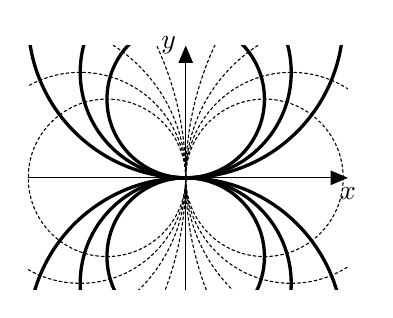
\begin{tikzpicture}[line cap=round,line join=round,>=triangle 45,x=1.0cm,y=1.0cm,scale=2.0]
				\draw[->,color=black] (-1,0) -- (1.03,0) node[below]{$x$};
				%\foreach \x in %{-1,-0.8,-0.6,-0.4,-0.2,0.2,0.4,0.6,0.8,1}
				%\draw[shift={(\x,0)},color=black] %(0pt,2pt) -- (0pt,-2pt) node[below] %{\tiny $\x$};
				\draw[->,color=black] (0,-0.71) -- (0,0.84) node[left]{$y$};
				%\foreach \y in %{-0.6,-0.4,-0.2,0.2,0.4,0.6,0.8}
				%\draw[shift={(0,\y)},color=black] %(2pt,0pt) -- (-2pt,0pt) node[left] %{\tiny $\y$};
				%\draw[color=black] (0pt,-10pt) %node[right] {\footnotesize $0$};
				\clip(-1,-0.71) rectangle (1.03,0.84);
				{
					\draw [line width=1.2pt] (0,-1) circle (1cm);
				}
				{
					\draw [line width=1.2pt] (0,-0.5) circle (0.5cm);
				}
				{
					\draw [line width=1.2pt] (0,-0.67) circle (0.67cm);
				}
				{
					\draw [line width=1.2pt] (0,1) circle (1cm);
				}
				{
					\draw [line width=1.2pt] (0,0.5) circle (0.5cm);
				}
				{
					\draw [line width=1.2pt] (0,0.67) circle (0.67cm);
				}
				{
					\draw [dash pattern=on 1pt off 1pt] (1,0) circle (1cm);
				}
				{
					\draw [dash pattern=on 1pt off 1pt] (0.67,0) circle (0.67cm);
				}
				{
					\draw [dash pattern=on 1pt off 1pt] (0.5,0) circle (0.5cm);
				}
				{
					\draw [dash pattern=on 1pt off 1pt] (2,0) circle (2cm);
				}
				{
					\draw [dash pattern=on 1pt off 1pt] (-2,0) circle (2cm);
				}
				{
					\draw [dash pattern=on 1pt off 1pt] (-1,0) circle (1cm);
				}
				{
					\draw [dash pattern=on 1pt off 1pt] (-0.5,0) circle (0.5cm);
				}
				{
					\draw [dash pattern=on 1pt off 1pt] (-0.67,0) circle (0.67cm);
				}
			\end{tikzpicture}
			\par\end{center}%
	\end{minipage}

	
	 \item \textcolor{red}{El semióvalo de Rankine}. Formado por una fuente (o
	sumidero) y un flujo uniforme. 
	\[
	\psi=U_{\infty}r\sin\theta+m\theta\quad;\quad\phi=U_{\infty}r\cos\theta+m\ln r
	\]
	
\begin{center}
	\includegraphics[width=0.7\linewidth]{../../MFGA/Presentaciones/21-ideal/rankine}
\end{center}

\end{itemize}

\section{Aerodinámica}

	
	Se habla de flujo externo cuando un cuerpo sólido se encuentra completamente
	sumergido en un flujo.
	
	En Flujo Ideal hemos visto las ecuaciones de Euler, cuando no se considera
	la viscosidad, y en flujo potencial cuando, además, el flujo es irrotacional.
	El flujo real se parece más al potencial (irrotacional) cuanto menor
	es el número de Reynolds)
\subsection{Flujo alrededor de un cilindro}
	
	\begin{center}
		\animategraphics[
		controls,scale=0.30
		]{1}{TeX_files/chapter09-Externo/Re}{0}{20}
	\end{center}
	

	
	Pero esto llevaba a la paradoja de D'Alembert, que se resolvía con
	la capa límite.
	
	Los flujo externos reales se estudian conectando ambos modelos: 
	\begin{description}
		\item [{flujo~ideal}] muy lejos del cuerpo, y que determina la forma del
		campo de velocidades y presiones alrededor de él, y 
		\item [{capa~límite}] muy cerca del cuerpo, que determina las fuerzas
		superficiales que actúan sobre él. 
	\end{description}
	En la zona intermedia, ambos modelos deben conectar de forma suave.
	
	La mayor parte de los resultados presentados en el estudio de flujos
	externos son o bien experimentales, o bien numéricos, dada la complejidad
	del problema.


\section{Fuerzas aerodinámicas}

	
	Un flujo externo produce sobre el cuerpo sólido una fuerza $\vec{F}$,
	denominada \textit{aerodinámica}, aunque el fluido no sea necesariamente
	aire.
	
	Esta fuerza se descompone en un sistema de coordenadas definido por
	la dirección del flujo ($x$) y una normal ($z$). La componente en
	la dirección del flujo, $F_{x}$ recibe el nombre de fuerza de arrastre,
	o, simplemente, \textit{arrastre}. En inglés, \textit{drag}, y, por
	esta razón tanto se encuentra escrita como $F_{x}$, como $F_{a}$,
	como $F_{d}$.
	
	La componente en la dirección normal, $F_{z}$, recibe el nombre de
	fuerza de sustentación, o, simplemente, \textit{sustentación}. En
	inglés \textit{lift}, y, por esta razón tanto se encuentra escrita
	como $F_{z}$, como $F_{s}$, como $F_{l}$.
	
	Es importante hacer dos comentarios: 
	\begin{enumerate}
		\item Ni la fuerza de arrastre tiene porqué ser horizontal ni la de sustentación
		vertical 
		\item La velocidad del viento incidente es la \textit{velocidad relativa}
		al cuerpo 
	\end{enumerate}
\begin{center}
	\includegraphics[width=\linewidth]{TeX_files/chapter09-Externo/plane}
\end{center}


\subsection{Arrastre de fricción y de presión}

	
	En el estudio de capa límite vimos cómo actúa la fricción (esfuerzo
	superficial) sobre una placa plana. Pero el arrastre también puede
	ser producido por una diferencia de presión entre la parte anterior
	y posterior del objeto.
	
	Consideremos el ejemplo de una esfera. Si $\Re<1$, no hay prácticamente
	separación, y el arrastre se produce casi por completo por fricción.
	Stokes calculó el valor de este arrastre, 
	
\begin{equation}
		F_{d}=3\pi\mu U_{\infty}D
\end{equation}
	
	
	Sin embargo, para $\Re$ mayores, el desprendimiento del flujo produce
	una zona de baja presión en la estela, y un reflujo en la misma. En
	estas condiciones, el arrastre se debe tanto a la fricción como a
	la presión.


\subsection{Coeficientes aerodinámicos}

	
	Como es habitual, se suelen utilizar magnitudes adimensionales para
	el estudio del flujo externo. La fuerza aerodinámica se compara con
	la presión dinámica del flujo lejano multiplicado por un área de referencia.
	
	El \textcolor{red}{coeficiente de arrastre} es 
	
\begin{equation}
		C_{d}=\dfrac{F_{d}}{\frac{1}{2}\rho U_{\infty}^{2}S_{x}}
\end{equation}
	
	donde $S_{x}$ es la sección proyectada por el cuerpo en la dirección
	del flujo.
	
	Para el \textcolor{red}{coeficiente de sustentación} 
\begin{equation}
		C_{l}=\dfrac{F_{l}}{\frac{1}{2}\rho U_{\infty}^{2}S}
\end{equation}
el área $S$ se define de forma diferente. 

	
	Dado que, para que un cuerpo tenga sustentación tiene que ser, normalmente,
	diseñado para ello (perfiles aerodinámicos), y el área $S_{x}$ varia
	mucho con la orientación del cuerpo, en estos casos, tanto para $C_{d}$
	como para $C_{l}$ se utiliza el área máxima proyectada del cuerpo,
	$S$.
	
	Los coeficientes de arrastre y de sustentación son coeficientes \textit{globales},
	en el sentido que describen el comportamiento del perfil en su totalidad.
	El \textcolor{red}{coeficiente de presión}, $C_{p}$, es un coeficiente
	\textit{local}, definido sobre la superficie del perfil. 
	
\begin{equation}
		C_{p}=\dfrac{p-p_{\infty}}{\frac{1}{2}\rho U_{\infty}^{2}}
\end{equation}
	
	

	
	Aplicando la ley de Stokes para el arrastre viscoso en una esfera,
	el coeficiente de arrastre es 
\begin{equation}
		C_{d}=\dfrac{24}{\Re}
\end{equation}
	
	Pero esto es válido únicamente para $\Re<1$. Para mayores números
	de Reynolds no hay una expresión analítica para $C_{d}$
	
	\begin{minipage}[c]{0.4\textwidth}%
\begin{center}
	\includegraphics[width=\linewidth]{TeX_files/chapter09-Externo/Cd_esphere}
\end{center}


	\end{minipage} %
	\begin{minipage}[c]{0.5\textwidth}%
		\smallskip{}
		
		Hasta $\Re\approx1000$, el arrastre se produce por combinación de
		la fricción y la presión, debido a la separación de la capa límite.
		A medida que aumenta $\Re$, disminuye la contribución de la fricción,
		de forma que para $\Re\approx1000$ es apenas el 5\% del arrastre
		total.%
	\end{minipage} 
	
	\begin{itemize}
		\item Para $10^{3}<\Re<3\times10^{5}$, la separación del flujo ocurre justo
		en la sección media de la esfera, y la presión en la estela, detrás
		de la esfera es prácticamente constante. Y, por lo tanto, también
		lo es $C_{d}$. La capa límite en la parte delantera de la esfera
		es laminar 
		\item Para $\Re>3\times10^{5}$, la capa límite en la parte delantera es
		turbulenta, y, por lo tanto, se resiste más al desprendimiento. El
		punto de separación se retrasa y esto produce una disminución de $C_{d}$
		debido a la menor sección expuesta a alto gradiente de presiones. 
	\end{itemize}

	
	\begin{minipage}[c]{0.4\textwidth}%
		Esta transición a capa límite turbulenta se puede provocar a menores
		números de Reynolds con la rugosidad de la superficie.
		
		Esta es la razón de la forma rugosa de las pelotas de golf %
	\end{minipage} %
	\begin{minipage}[c]{0.5\textwidth}%
		De Munson\cite{Munson}:
\begin{center}
	\includegraphics[width=\linewidth]{TeX_files/chapter09-Externo/roughSphere.png}
\end{center}
	\end{minipage}
	
	\smallskip{}
	En el caso de un \textbf{cilindro} (flujo bidimensional) la curva
	$C_{d}-\Re$ es muy parecida, aunque $C_{d}$ es aproximadamente el
	doble.\smallskip{}
	
	\begin{minipage}[c]{0.4\textwidth}%
\begin{center}
	\includegraphics[width=\linewidth]{../../MFGA/Presentaciones/22-externo/von_karman}
\end{center}
	\end{minipage} %
	\begin{minipage}[c]{0.58\textwidth}%
		La simetría del cilindro puede provocar la aparición de una serie
		de vórtices uniformemente espaciados en la estela, producidos por
		el desprendimiento alternativo del flujo. Se conoce como estela de
		vórtices o \textit{calle de von Kármán}, y aparece para $60<\Re<5000$. %
	\end{minipage}

	
	Esta estela la responsable de la oscilación de las banderas, del zumbido
	de los cables. Se pueden eleminar con elementos que destruyan la simetría.
	Para $\Re>1000$ el número de Strouhal ($\textrm{St}\equiv\frac{fD}{V_{\infty}}$)
	de esta calle de vórtices es aproximadamente 0,21. 
	
	\begin{center}
		\includegraphics[width=\linewidth]{../../MFGA/Presentaciones/22-externo/strouhal-reynolds}
	\end{center}
	
	

	
	\subsection*{Actividad 1:}
		Una chimenea cilíndrica de 1 m de diámetro y 25 metros de alto está
		expuesta a un viento uniforme de 50 km/h en condiciones atmosféricas
		estándar. Los efectos de los extremos se pueden despreciar. 
		
		Estimar el momento de flexión en la base de la chimenea debido a la
		fuerza del viento.
		
		Estimar la frecuencia de los vórtices de von Kármán creados en la
		chimenea.


	

		En esta tabla se presentan algunos $C_{d}$ de cuerpos 2D y 3D, para
		$\Re\gtrsim10^{3}$. Dado que el arrastre se produce mayoritariamente
		por presión, el coeficiente es prácticamente constante.%

\begin{center}
	\includegraphics[width=0.6\linewidth]{../../MFGA/Presentaciones/22-externo/drag-shapes}
\end{center}


	
	\subsection*{Actividad 2:}
		Un coche de competición, con una masa de 1000 Kg, que circula con
		una velocidad de 350 km/h frena con un paracaidas de 3 m$^{2}$. Estima
		el tiempo y la distancia necesarios para reducir la velocidad a la
		mitad.
		
		Nota: Un paracaídas se puede aproximar a una semiesfera abierta contra
		el viento. 


\subsection{Perfil aerodinámico}

	
	Si se hace un fuselaje a un cilindro en la parte trasera se puede
	evitar el desprendimiento del flujo. Por otro lado, se aumenta el
	área y, por lo tanto, el arrastre por fricción. La forma óptima de
	un perfil aerodinámico es la que minimiza el arrastre total, con una
	gran sustentación.
	
	Definiciones: 
	\begin{itemize}
		\item \textcolor{red}{cuerda}: linea recta que une el borde delantera y
		el borde posterior del perfil. Normalmente se denomina así también
		a su longitud. 
		\item \textcolor{red}{linea media}: linea formada por los puntos medios
		entre curva superior (extradós) y curva inferior (intradós) del perfil,
		según la perpendicular a ella misma. Los perfiles NACA son normalmente
		diseñados combinando una linea media y una distribución de espesor.
		Si la linea media es recta y coincide con la cuerda,se dice que el
		perfil es simétrico. 
	\end{itemize}

	
	Una característica importante de un perfil aerodinámico es el lugar
	de la cuerda en el que se encuentra el espesor máximo. Si este punto
	se retrasa hacia el borde de fuga, el flujo se mantiene laminar gracias
	al gradiente favorable de presión.
	
	Este tipo de perfil  \textit{laminar} tiene muy
	poco arrastre, pero, por otro lado, es más susceptible de entrar en
	pérdida.
	
	Los coeficientes aerodinámicos dependen del ángulo de ataque, que
	es el ángulo que forman la cuerda y la dirección del flujo externo
	no perturbado.
	
	Cuando el perfil está en pérdida, el flujo está completamente desprendido
	en el extradós, y el perfil se hace inestable, bajando $C_{l}$, y
	aumentando considerablemente $C_{d}$. 

\begin{center}
	\includegraphics[width=0.6\linewidth]{../../MFGA/Presentaciones/22-externo/cl}
\end{center}

\begin{center}
	\includegraphics[width=0.7\linewidth]{../../MFGA/Presentaciones/22-externo/perdida}
\end{center}
	

\chapter[Flujo en tuberías]{Flujo interno en tuberías}
\section{La ecuación de Darcy-Weisbach}
Cuando un fluido pasa por una tubería pierde energía debido a la fricción con las paredes. ésta pérdida de energía se mide normalmente como una pérdida de presión, ya que la velocidad está determinada por el caudal. Pero en realidad, se pierde una parte de la energía total, como se indica en la \textcolor{blue}{ecuación de Bernoulli generalizada}.

\begin{equation}
	p_1 + \frac{1}{2}\rho v_1^2 + \rho g z_1 = p_2 + \frac{1}{2}\rho v_2^2 + \rho g z_2 + \Delta p_f
\end{equation}


La pérdida de presión $\Delta p_f$ dependerá de la longitud $L$, el diámetro $D$ y la rugosidad $e$ de las paredes de la tubería y, por otra parte, de la velocidad media $v$, la densidad $\rho$ y la viscosidad $\mu$ del fluido,

\begin{equation}
	\Delta p_f = f(L,D,e,v,\rho,\mu).
\end{equation}

Son 7 variables. Del Teorema $\Pi$ de Buckingham sabemos que podemos reducirlas a 4 grupos adimensionales. La forma convencional de hacerlo es

\begin{equation}
	\frac{\Delta p_f}{\frac{1}{2} \rho v^2} = f\Bigl(\frac{L}{D},\frac{e}{D},\frac{\rho v D}{\mu}\Bigr)
\end{equation}


Es lógico pensar, y se comprueba experimentalmente, que ésta pérdida de presión ha de ser proporcional a la longitud $L$ de la tubería, de forma que

\begin{equation}
	\frac{\Delta p_f}{\frac{1}{2} \rho v^2} = \frac{L}{D} f\Bigl(\frac{e}{D},\frac{\rho v D}{\mu}\Bigr)
\end{equation}


$\frac{e}{D} = \varepsilon$ es la \textcolor{blue}{rugosidad relativa} de la tubería y $\frac{\rho v D}{\mu} = \re_D $ es el \textcolor{blue}{número de Reynolds} del flujo. y la expresión

\begin{equation}
	\boxed{
	\frac{\Delta p_f}{\frac{1}{2} \rho v^2} = \frac{L}{D} f(\varepsilon,\re_D)
}
\end{equation}

es la \textcolor{red}{ecuación de Darcy-Weisbach} (1850). $f$ es el \textcolor{red}{factor de fricción de Darcy}.


A veces es conveniente expresar la ecuación de Darcy-Weisbach en términos  de pérdida de altura, en lugar de pérdida de presión, $\Delta h_f = \frac{\Delta p}{\rho g}$,

\begin{equation}
	\Delta h_f = f(\varepsilon,\re_D) \frac{L}{D} \frac{1}{2g}v^2.
\end{equation}


\begin{center}
	\includegraphics[scale=0.9,angle=270]{TeX_files/chapter10-Tuberias/alturas1.pdf}
\end{center}

\section{Flujo laminar}
Cuando $\re_D$ es pequeño (menor que aproximadamente 2300), en la tubería tenemos un flujo de Poiseuille, estudiado en el tema sobre Flujo Viscoso,

\begin{equation}
	v_x(r) = -\deriv{p}{x}\frac{1}{4\mu}\bigl(R^2 - r^2\bigr),
\end{equation}

donde ahora consideramos que el eje de la tubería está en la dirección $x$, y no hay variación de altura $z$.

$-\deriv{p}{x} = \frac{\Delta p_f}{L}$, y el hecho de que $\Delta p_f$ sea considerada una pérdida ya implica el signo negativo de la derivada,

\begin{equation}
	v_x(r) =  \frac{\Delta p_f}{L}\frac{1}{4\mu}\bigl(R^2 - r^2\bigr)
\end{equation}


La velocidad media del flujo es

\begin{equation}
	v = \frac{1}{S}\int_S v_x \dif S = \frac{1}{\pi R^2}\int_0^R v_x(r) 2\pi r \dif r = \frac{\Delta p_f}{L}\frac{R^2}{8\mu}.
\end{equation}

Vamos a ver cuánto vale $f$ en este caso,
\[\frac{1}{2g}v^2 = \frac{\Delta p_f}{L}\frac{R^2 v}{16\mu g} = \frac{\Delta p_f}{\rho g}\frac{D}{L}\frac{ \rho D v}{64\mu}\]
\[\frac{\Delta p_f}{\rho g} = h_f =\frac{64\mu}{ \rho D v}\frac{L}{D}\frac{1}{2g}v^2 \]

Por lo tanto,

\begin{equation}
	\boxed{
	f=\frac{64\mu}{ \rho D v} = \frac{64}{Re_D}
}
\end{equation}
que no depende de la rugosidad del material de la tubería.

\textbf{Ejemplo 1: }

Un aceite de densidad $\rho = 900 \,\text{Kg}/\text{m}^3$ y viscosidad $\nu = 2\times 10^{-4} \, \text{m}^2/\text{s}$ fluye hacia arriba por una tubería inclinada de 6 cm de diámetro, como se indica en la figura. Las presiones en los puntos 1 y 2, separados 10 metros, son $p_1 = 3.5\times10^5\,\text{Pa}$ y $p_2 = 2.5\times10^5\,\text{Pa}$, respectivamente. Vamos a calcular el caudal que circula por la tubería.

\begin{center}
	\input{TeX_files/chapter10-Tuberias/ejemplo1.eepicemu}
\end{center}

La ecuación de Bernoulli generalizada es
\[
p_1 + \frac{1}{2}\rho v_1^2 + \rho g z_1 = p_2 + \frac{1}{2} \rho v_2^2 + \rho g z_2 + \Delta p_f.
\]
Dado que no hay cambio de sección, $v_1 = v_2$, y la ecuación queda como
\[
p_1 + \rho g z_1 = p_2 + \rho g z_2 + \Delta p_f
\]
\[
\Rightarrow \, \Delta p_f = p_1 - p_2 + \rho g (z_1 - z_2) = \Delta p - \rho g L \sin \beta
\]

Supongamos que el flujo es laminar. En este caso,
\[
\Delta p_f  = f \frac{L}{D} \frac{1}{2} \rho v^2 = \frac{64}{\re_D} \frac{L}{D} \frac{1}{2} \rho v^2 = \frac{64 \nu}{v D} \frac{L}{D} \frac{1}{2} \rho v^2 =
\frac{32 \nu \rho L v}{D^2}.
\]
Igualando las dos expresiones,
\[
\frac{32 \nu \rho L v}{D^2} = \Delta p - \rho g L \sin \beta \, \Rightarrow \, v = \frac{D^2}{32 \nu \rho L} (\Delta p - \rho g L \sin \beta)
\]

Haciendo las operaciones obtenemos $v = 2.7 \, \text{m}/\text{s}$ y,
\[
Q = v \pi R^2 = 7.65\times10^{-3}\,\text{m}^3/\text{s}
\]

\section{Flujo turbulento en tubería lisa}
Supongamos que el perfil de velocidades sigue la ley logarítmica en toda la sección de la tubería\footnote{Ver capítulos sobre Turbulencia y Capa Límite.},

\begin{equation}
	\frac{v_x(r)}{v^*} \approx \frac{1}{\kappa}\ln \frac{(R-r)v^*}{\nu} + B,
\end{equation}

donde $(R-r)$ es la distancia hasta la pared.

\begin{center}
	\input{TeX_files/chapter10-Tuberias/turbulento1.eepicemu}
\end{center}


La velocidad media es
\[v = \frac{1}{S} \int_S v_x(r) \dif S = \frac{v^*}{\pi R^2}
\int_0^R \left[\frac{1}{\kappa}\ln \frac{(R-r)v^*}{\nu} + B\right] 2\pi r \dif r
\]

\begin{equation}
	v = \frac{v^*}{2} \left[\frac{2}{\kappa} \ln \frac{R v^*}{\nu} + 2B - \frac{3}{\kappa} \right]
\end{equation}

Si introducimos los valores conocidos $\kappa = 0.41$, $B=5.0$, obtenemos

\begin{equation}
	\frac{v}{v^*} = 2.44 \ln \frac{R v^*}{\nu} + 1.34
\end{equation}


La relación de esta velocidad media $v$ con la pérdida de presión en la tubería $\Delta p_f$ viene dada a través de $v^* = \sqrt{\frac{\tau_p}{\rho}}$.


Aplicando conservación de cantidad de movimiento sobre le Volumen de Control de la figura, considerando que el flujo es horizontal (no hay efectos de la gravedad) y estacionario, tenemos
\[
- p_1 S_1 + p_2 S_2 - \tau_p 2\pi R L = \dot{m}(v_2-v_1) = 0
\]
\[
\Rightarrow \, \Delta p_f \pi R^2 - \tau_p 2\pi R L = 0 \,
\Rightarrow \, \tau_p = \Delta p_f \frac{R}{2 L}
\]
de forma que la velocidad de fricción $v^*$ es

\begin{equation}
	v^* = \sqrt{\frac{\Delta p_f R}{2 \rho L}},
\end{equation}

y

\begin{equation}
	\frac{v}{v^*} = \frac{v}{\sqrt{\frac{\Delta p_f R}{2 \rho L}}} = \sqrt{\frac{2 \rho v^2 L}{R \Delta p_f}} = \sqrt{\frac{4 \rho v^2}{\Delta p_f}\frac{L}{D}} =
\sqrt{8\frac{1/2 \rho v^2}{\Delta p_f}\frac{L}{D}} = \sqrt{\frac{8}{f}}
\end{equation}


Por otro lado,
\[
\frac{R v^*}{\nu} = \frac{R}{\nu} \frac{v}{\sqrt{\frac{8}{f}}} = \frac{R v}{\nu}
\sqrt{\frac{f}{8}}= \frac{1}{2}\frac{D v}{\nu}\sqrt{\frac{f}{8}} = \frac{1}{2}\re_D\sqrt{\frac{f}{8}}
\]

De forma que podemos transformar la relación de la velocidad media $V$ en función de $v^*$ en una relación del factor de fricción $f$ en función de $\re_D$,

\begin{equation}
	\sqrt{\frac{8}{f}} = 2.44 \ln \left[\frac{1}{2}\re_D \sqrt{\frac{f}{8}}\right] + 1.34,
\end{equation}

que se suele expresar en términos de logaritmo en base 10, y con las constantes ajustadas para concordar con los experimentos, dando la \textcolor{red}{ecuación de Prandtl},

\begin{equation}
	\boxed{
	\frac{1}{\sqrt{f}} = 2.0\log \left[ \re_D \sqrt{f}\right] - 0.8
}
\end{equation}

Una relación explícita aproximada dada por Blasius es

\begin{equation}
	f = \frac{0.316}{\re_D^{1/4}}
\end{equation}

\begin{center}
	\includegraphics[scale=.45]{TeX_files/chapter10-Tuberias/f1.pdf}
\end{center}

\section{Flujo turbulento en tubería rugosa}

Nikuradse estudió el efecto que tiene la rugosidad de la tubería sobre el flujo turbulento, descubriendo que cuando la variable adimensional
$e^+ = \frac{e v^*}{\nu}$ es mayor que 70, el efecto sobre el flujo es indepediente de $\re_D$, y la velocidad en la ley logarítmica se reduce en una cantidad $\frac{1}{\kappa}\ln e^+ - 3.5$,
\[
\frac{v_x(r)}{v^*} = \frac{1}{\kappa}\ln \frac{(R-r) v^*}{\nu} + B - \bigl( \frac{1}{\kappa}\ln \frac{e v^*}{\nu}- 3.5\bigr) = \frac{1}{\kappa}\ln \frac{(R-r)}{e} + 8.5.
\]
Repitiendo el análisis anterior calculando  la velocidad media se llega a la relación entre $f$ y $\varepsilon$ con flujo completamente rugoso, en la que no hay dependencia con $\re_D$,
\[
\frac{v}{v^*} = -2.0\ln \frac{D}{e} + 3.2
\]

\begin{equation}
	\Rightarrow \,
\boxed{
	\frac{1}{\sqrt{f}} = -2.0 \log \frac{\varepsilon}{3.7}
}
\end{equation}

Más tarde Colebrook llegó a la expresión general que combinaba la relación para tubería lisa, y la del flujo completamente rugoso,

\begin{equation}
	\boxed{
	\frac{1}{\sqrt{f}} = -2.0 \log \left( \frac{\varepsilon}{3.7} + \frac{2.51}{\re_D \sqrt{f}} \right)
}
\end{equation}

y todas estas expresiones fueron condensadas en el \textcolor{red}{diagrama de Moody} que es la herramienta normalmente usada para el cálculo de pérdidas de presión en tuberías.

Indicación de algunas rugosidades típicas de materiales comunes usados en la construcción de tuberías

\begin{tabular}{|c|c|}
	\hline \textbf{Material}  & \textbf{rugosidad (mm)} \\
	\hline
	\hline Acero inox. nuevo & 0.002 \\
	\hline Acero comercial & 0.046 \\
	\hline Acero oxidado & 2.0 \\
	\hline Hierro de fundición & 0.26 \\
	\hline Hierro forjado & 0.046 \\
	\hline
\end{tabular}
\begin{tabular}{|c|c|}
	\hline \textbf{Material}  & \textbf{rugosidad (mm)} \\
	\hline
	\hline Hierro galvanizado & 0.15 \\
	\hline Fundición alfaltado & 0.12 \\
	\hline Hormigón  & 0.04 - 2.0 \\
	\hline Plástico & 0.0015 \\
	\hline Latón & 0.002 \\
	\hline
\end{tabular}
\newpage
\vspace*{-3cm}
\includegraphics[scale=0.85,angle=90]{TeX_files/chapter10-Tuberias/moody.pdf}
\newpage
\textbf{Ejemplo :}

Queremos calcular la pérdida de presión en una tubería de fundición asfaltada de 150 mm de diámetro y 50 metros de longitud por la que circula agua con una velocidad media de 2,5 m/s.

En primer lugar calculamos $\re_D$ y la rugosidad relativa,
\[\re_D = \frac{v D}{\nu} = \frac{2.5\times 0.15}{10^{-6}} = 3.75\times10^5\]
\[\varepsilon = \frac{e}{D} = \frac{0.12}{150} = 8\times10^{-4}\]

Con estos valores estamos en la zona de flujo turbulento, aunque no es completamente rugoso, de forma que el factor de fricción va a venir dado por
\[
\frac{1}{\sqrt{f}} = -2.0 \log \left( \frac{\varepsilon}{3.7} + \frac{2.51}{\re_D \sqrt{f}} \right) = -2.0 \log \left( 2.162\times10^{-4} + \frac{6.693\times10^{-6}}{\sqrt{f}}\right)
\]

Hay, por lo menos, dos formas de resolver esta ecuación.

La primera es mediante un proceso iterativo. Iniciamos el cálculo con una aproximación de $f$ que podemos obtener del diagrama de Moody. Por ejemplo, $f_0=0.019$. Calculamos $f_1$ mediante
\[\frac{1}{\sqrt{f_1}} = -2.0 \log \left( 2.162\times10^{-4} + \frac{6.693\times10^{-6}}{\sqrt{f_0}}\right)\,\rightarrow\, f_1 = 0.01954
\]
y seguimos iterando
\[\frac{1}{\sqrt{f_2}} = -2.0 \log \left( 2.162\times10^{-4} + \frac{6.693\times10^{-6}}{\sqrt{f_1}}\right)\,\rightarrow\, f_2 = 0.01953
\]
hasta que obtenemos una convergencia suficiente.

La segunda es con una calculadora que resuelva ecuaciones de forma implicita (el proceso es el mismo, pero lo hace la calculadora de una forma mucho más rápida).

El valor correcto es $f= 0.01953$, de forma que la pérdida de presión es
\[\Delta p_f = f \frac{L}{D} \frac{1}{2}\rho v^2 = 0.01953 \times \frac{50}{0.15}\times\frac{1}{2}\times1000\times2.5^2 = 20340 \, \text{Pa}\]

\section{Cálculo de caudales}
Calcular la pérdida de presión $\Delta p_f$ a partir de los datos de la geometría de la tubería y las propiedades del fluido y su caudal es fácil.

Más interesante es calcular el caudal conocida la pérdida de presión. La forma de resolver este tipo de problemas es mediante un proceso iterativo, en el que se inicia considerando que el flujo es completamente rugoso, de forma que $f$ no dependa de $\re_D$
\[
\frac{1}{\sqrt{f_0}} = -2.0 \log \frac{\varepsilon}{3.7}
\]

Una vez tenemos $f$, calculamos la velocidad con
\[
\Delta p_f = f_0 \frac{L}{D} \frac{1}{2}\rho v_0^2
\]
y, de aquíel caudal.

Con esta velocidad se calcula ${\re_D}_0 = \frac{v_0 D}{\nu}$ y verificamos si el flujo es totalmente rugoso. Si es as\'{\i}, el problema está terminado. Si no, tenemos que volver a calcular $f_1$ mediante la expresión de Colebrook
\[
\frac{1}{\sqrt{f_1}} = -2.0 \log \left(\frac{\varepsilon}{3.7} + \frac{2.51}{\re_D \sqrt{f_1}}\right)
\]
e iterar hasta obtener la convergencia.

\textbf{Ejemplo : }

En una tubería de fundición asfaltada de 150 mm  de diámetro y 20 metros de largo, circula agua y la pérdida de presión es de 4 m.c.a. Queremos saber cuánto es el caudal de agua.

Suponemos flujo completamente rugoso con
\[\varepsilon = \frac{e}{D} = \frac{0.12}{150} = 8.0\times10^{-4}\]
y calculamos $f_0$,
\[
\frac{1}{\sqrt{f_0}} = -2.0 \log \frac{8.0\times10^{-4}}{3.7} \, \rightarrow \, f_0 = 0.0186
\]

El primer valor tentativo de la velocidad del flujo vendrá dado por
\[
\rho g h_f = f_0 \frac{L}{D}\frac{1}{2}\rho v_0^2
\]
\[
v_0 = \sqrt{\frac{g h_f 2 D}{f_0 L}} \, \rightarrow \, v_0 = 5.62 \, \text{m/s}.
\]

Calculamos el número de Reynolds
\[
{\re_D}_0 = \frac{v_0 D}{\nu}= 8.43\times 10^5
\]

Con este valor, no estamos en flujo completamente rugoso. De forma que volvemos a calcular el factor de fricción y la velocidad
\[
\frac{1}{\sqrt{f_1}} = -2.0 \log \left(\frac{8.0\times10^{-4}}{3.7}+\frac{2.51}{8.43\times 10^5\sqrt{f_1}}\right)
\]
\[
\rightarrow f_1 = 0.0190 \,\rightarrow \, v_1 = 5.56 \, \text{m/s}
\]

Si el grado de exactitud que se requiere no es muy elevado, podemos quedarnos con $v=5.6\,\text{m/s}$ y $Q=v\pi D^2/4 = 0.1 \, \text{m}^3/\text{s}$.

\section{Dimensionamiento de tuberías}

A veces se quiere saber cuál es el diámetro necesario de una tubería que debe llevar un determinado caudal con una pérdida de presión determinada. El problema no es sencillo, ya que para poder calcular $f$ es necesario $\re_D$ y $\varepsilon$, y los dos dependen del diámetro $D$.

Debemos de usar de nuevo un proceso iterativo. Iniciamos con un valor de $f$. Un valor típico és $f_0=0.02$.

A partir de este valor de $f$ calculamos el diámetro mediante
\[
\Delta p_f = f_0 \frac{L}{D}\frac{1}{2}\rho v_0^2 = \frac{8 f_0 \rho L Q^2}{\pi^2 D_0^5}
\]
\[
\Rightarrow  \, D_0 = \sqrt[5]{\frac{8 \rho f_0 L Q^2}{\pi^2 \Delta p_f}}
\]

Con este valor de $D_0$ calculamos $\varepsilon_0$ y ${\re_D}_0 = \frac{v_0 D_0}{\nu} = \frac{4 Q}{\pi D_0 \nu}$, y con estos valores  calculamos $f_1$, y continuamos el proceso iterativo hasta conseguir la convergencia deseada.

\textbf{Ejemplo : }

En el ejemplo anterior, queremos que el caudal sea el doble. ?` Cuál tendrá que ser el diámetro ?

Queremos que $Q=0.2\,\text{m}^3/\text{s}$. Iniciamos el proceso con $f_0=0.02$, y obtenemos
\[
D_0 = \sqrt[5]{\frac{8 \rho f_0 L Q^2}{\pi^2 \rho g h_f}} =
\sqrt[5]{\frac{8 f_0 L Q^2}{\pi^2 g h_f}} = 0.201\,\text{m}
\]

\[
\varepsilon_0 = \frac{e}{D_0} = \frac{0.12}{0.201} = 5.96\times10^{-4}
\]
\[
{\re_D}_0 = \frac{4 Q}{\pi D_0 \nu} = 1.27\times10^6
\]
\[
\frac{1}{\sqrt{f_1}} = -2.0 \log \left(\frac{5.96\times10^{-4}}{3.7}+\frac{2.51}{1.27\times 10^6\sqrt{f_1}}\right)
\, \rightarrow \, f_1 = 0.0177
\]
\[
D_1 = \sqrt[5]{\frac{8 f_1 L Q^2}{\pi^2 g h_f}} = 0.197\,\text{m}
\]
y seguiríamos quizás con una segunda iteración. Al final, de todas formas, hemos de escoger un medida de diámetro normalizada. En nuestro caso, 200 mm.

\section{Conductos no circulares}

Cuando el conducto no es circular los cálculos son más o menos los mismos, pero se complica un poco el álgebra.

Como medida equivalente al radio de la tubería se usa el concepto de \textcolor{red}{radio hidráulico}, definido como la relación entre la sección de paso del flujo y el perímetro mojado en el conducto

\begin{equation}
	R_h = \frac{A}{P}
\end{equation}


donde hay que tener en cuenta que $P$ es todo el perímetro en el que haya esfuerzo tangencial.

La pérdida de presión se calcula entonces como
\[
\Delta p_f = f \frac{L}{D_h} \frac{1}{2} \rho v^2
\]
donde $D_h = 4 R_h$ es el \textcolor{red}{diámetro hidráulico}, y $f$ es función de nuevo de la rugosidad relativa, $\varepsilon= e/D_h$ y el número de Reynolds se calcula como

\begin{equation}
	{\re_D}_h = \frac{v D_h}{\nu}.
\end{equation}


Por desgracia, para el cálculo de $f$ no sirven las expresiones deducidas para los conductos circulares ni el diagrama de Moody, aunque dan un valor bastante aproximado (dentro del 15\%) para flujo turbulento. Para flujo laminar el error es mayor, pero, por otro lado, el cálculo directo es más sencillo.

\textbf{Ejemplo : }

Calcular el factor de fricción $f$ para el flujo en un conducto rectabgular mucho mas ancho que alto ($b \gg h$) para flujo laminar y comparar con $f=64/\re_D$.

En este caso podemos considerar el flujo como el producido entre dos placas paralelas separadas por una distancia $h$. Sabemos que la distribución de velocidades es una parábola. Con el eje $z$ según la dirección del flujo y el eje $y$ perpendicular a las placas, tenemos
\[
v_z(y) = \frac{1}{\mu}\frac{\Delta p}{L}\left[y h -y^2\right]
\]

La velocidad media es
\[
v = \frac{1}{h}\int_0^h\frac{1}{\mu}\frac{\Delta p}{L}\left[y h -y^2\right] \dif y =
\frac{1}{12 \mu}\frac{\Delta p}{L} h^2
\]

Suponiendo que la velocidad es constante y que no hay ningún otro tipo de aporte o consumo de presión (gravedad, bombas, etc\ldots), la variación de presión $\Delta p$ és la pérdida de presión por fricción, $\Delta p_f$,
\[
\Delta p_f = \frac{12 \mu L v} {h^2}
\]

Vamos a relacionarlo con el número de Reynolds, que se define como
\[
\re_{D_h} = \frac{\rho D_h v}{\mu}
\]
donde $D_h = 4R_h = 4bh/(2a+2b)=2h$ si consideramos la aproximación $b \gg h$, de forma que, eliminado $\mu$ entre $\re_{D_h}$ y $\Delta p_f$, obtenemos
\[
\Delta p_f = \frac{24 \rho L v^2}{h\re_{D_h}} = \frac{96}{\re_{D_h}} \frac{L}{D_h} \frac{1}{2}\rho v^2
\]
es decir, $f ={96}/{\re_{D_h}}$, un 50\% más alto de lo correspondiente a un conducto circular.  La razón es que para un mismo diámetro hidráulico, un rectángulo siempre tiene mayor perímetro y, por lo tanto, mayor zona de actuación del esfuerzo tangencial de pared.


Para un conducto rectangular con $b \approx h$ el cálculo es mucho más complicado. Se suele usar entonces el concepto de \textcolor{red}{diámetro efectivo}, que es el diámetro que habría de tener un conducto circular que, en régimen laminar, tuviese la misma pérdida de carga con la misma velocidad media. Ya que para un conducto circular,

\begin{tabular}{lc}
	\begin{minipage}{0.5\textwidth}
		\[
		\Delta p_f = \frac{64}{\re}\frac{L}{D_e}\frac{1}{2}\rho v^2
		\]
		obtenemos
		\[
		\frac{64}{\re}\frac{L}{D_e}\frac{1}{2}\rho v^2 = f \frac{L}{D_h}\frac{1}{2}\rho v^2
		\]
		\[
		\Rightarrow \, D_e = \frac{64}{f \re} D_h
		\]
		donde $f\re$ se determina a partir de cálculos de la teoría laminar. éste diámetro se usa entonces también el cálculo de $f$ con flujo turbulento.
		
		\medskip 
		
	\end{minipage}
	&
	\begin{minipage}{0.4\textwidth}
		\begin{center}
			\begin{tabular}{|c|c|}
				\hline b/h & $f\re$ \\
				\hline
				\hline 0.0 & 96.00 \\
				\hline 0.05 & 89.91 \\
				\hline 0.1 & 84.68 \\
				\hline 0.125 & 82.34 \\
				\hline 0.167 & 78.81 \\
				\hline 0.25 & 72.93 \\
				\hline 0.4 & 65.47 \\
				\hline 0.5 & 62.19 \\
				\hline 0.75 & 57.89 \\
				\hline 1.0 & 56.91 \\
				\hline
			\end{tabular}
		\end{center}
	\end{minipage}
\end{tabular}

\bigskip

\textbf{Ejemplo : }

Por un conducto rectangular de $200\times 150$ mm y 30 metros de largo, con una rugosidad $e=0.1$~mm, circulan $0.7\, \text{m}^3/\text{s}$ de aire a $20^\circ C$ y 1 atmósfera de presión. Calcular la pérdida de presión.

La velocidad media del flujo es
\[
v = \frac{0.7}{0.03} = 23,3 \, \text{m/s}
\]
y el diámetro hidráulico es
\[
D_h = 4\frac{A}{P}=4\frac{ab}{2(a+b)}=\frac{2ab}{a+b}=171.43\,\text{mm}
\]

El diámetro efectivo es, de la tabla de $f\re$,
\[
D_e = \frac{64}{57.89}D_h = 189.5\,\text{mm}.
\]

Con este diámetro calculamos el factor de fricción,
\[
\re_{D_e}=\frac{v D_e}{\nu} = 2.5\times 10^5
\]
\[
\varepsilon = \frac{e}{D_e}=\frac{0.1}{189.5}=5.3\times10^{-4},
\]
usando el diágrama de Moody, $f=0.0185$, y la pérdida de presión
\[
\Delta p_f = f \frac{L}{D_e}\frac{1}{2}\rho v^2= 0.0185\times \frac{30}{0.1895}\times\frac{1}{2}1.2\times23.3^2 = 954\,\text{Pa}
\]

Si hubiésemos hecho el cálculo sin la corrección del diámetro efectivo, directamente con $D_e$, habríamos obtenido $\Delta p_f = 1087\,\text{Pa}$, es decir, un 15\% más grande. 

\section{Pérdidas de carga secundarias}

Además de la pérdida de carga provocada por fricción con las paredes de las tuberias y conductos, existen tamibén las {\it pérdidas de carga de forma, o secundarias}, creadas en puntos concretos de la instalación donde el flujo sufre cambios bruscos de módulo y/o dirección de la velocidad. Esto puede darse en:
\begin{itemize}
	\item Codos
	\item T's
	\item Bifurcaciones
	\item Válvulas
	\item Entradas/salidas de depósitos
	\item Filtros
	\item Toberas/difusores
	\item etc\ldots
\end{itemize}  

La pérdida de carga en estos elementos se caracteriza mediante el \textit{coeficiente de pérdidas secundarias}

\begin{equation}
	k = \frac{\Delta p_s}{\frac{1}{2}\rho v^2}
\end{equation}

donde $v$ es la velocidad del flujo en la tuber\'ia asociada al elemento.

Debido a la gran variedad de geometr\'ias y a la complejidad del flujo, no hay una teor\'ia que permita calcular el valor de $k$. éste viene dado por tablas o gráficas experimentales que a menudo, como en el caso de las válvulas, són facilitadas por el fabricante.

En general, se considera que el flujo es turbulento.


\begin{minipage}{10cm}
	Como ejemplo, mostramos el valor de $k$ para un codo de $45^\circ$, $90^\circ$ y $180^\circ$ en función de la relación entre el diámetro de la tuber\'ia $d$ y el radio de curvatura del codo$R$ 
	
	La forma de las gráficas es debida al efecto conjunto de la pérdida de carga primaria, que aumenta con $R/d$ y la secundaria, que disminuye.
	\medskip
	\begin{center}
		\includegraphics{TeX_files/chapter10-Tuberias/codo.pdf}
		% codo.eps: 300dpi, width=0.98cm, height=0.79cm, bb=0 0 116 93
	\end{center}
\end{minipage}
\begin{minipage}{10cm}
	\begin{center}
		\includegraphics[width=5cm]{TeX_files/chapter10-Tuberias/k-codo.png}
		% k-codo.png: 200dpi, width=2.87cm, height=3.30cm, bb=0 0 226 260
	\end{center}
\end{minipage}

\begin{minipage}{10cm}
	En la salida brusca a un depósito, independientemente de la forma de ésta, $k=1$, debido a que, simplemente, se pierde la presión dinámica que lleva el flujo en la tuber\'ia. 
	
	Sin embargo, en la \textit{entrada de un depósito a una tuber\'ia}, el valor de $k$ depende fuertemente de la geometr\'ia, como se puede observar en las gráficas.
	\medskip
	\begin{center}
		\includegraphics{TeX_files/chapter10-Tuberias/entrada_deposito.pdf}
	\end{center}
\end{minipage}
\begin{minipage}{10cm}
	\begin{center}
		\includegraphics[scale=0.5]{TeX_files/chapter10-Tuberias/k-entrada-deposito.png}
	\end{center}
\end{minipage}

En una expansión, o contracción brusca, el valor de $k$ depende de la relación de diámetros de las tuber\'ias. En el caso de la expansión, el esfuerzo tangencial producido en la zona de aguas muertas es negligible, y un análisis simple de conservación de cantidad de movimiento y energ\'ia lleva a la expresión

\begin{minipage}{10cm}
	\[
	k = \left(1 - \frac{d^2}{D^2}\right)^2
	\]
	
	Para la contracción brusca, el flujo que llega de la tuber\'ia grande se contrae por debajo del diámetro de la tuber\'ia peque\~na, dando lugar a la vena contracta. Experimentalmente se encuentra que
	\[
	k \approx 0.42 \left(1 - \frac{d^2}{D^2}\right)
	\]
	si $d/D$ no es muy cercano a 1.
\end{minipage}
\begin{minipage}{10cm}
	\begin{center}
		\includegraphics[scale=0.5]{TeX_files/chapter10-Tuberias/k-epansion-contraccion.png}
	\end{center}
\end{minipage}


Si la contracción es gradual, las pérdidas de carga secundarias son muy peque\~nas, y se pueden aproximar por los valores experimentales
\begin{center}
	% use packages: array
	\begin{tabular}{|c||c|c|c|}\hline
		$2\theta$ & 30 & 45 & 60 \\ \hline
		$k$ & 0.02 & 0.04 & 0.07 \\ \hline
	\end{tabular}
\end{center}

\begin{minipage}{10cm}
	Para una expansión gradual, también conocida como difusor, el valor de $k$ es como se muestra en la figura.
	
	El papel de un difusor es aumentar la presión estática del flujo. Esta caracter\'istica viene dada por el coeficiente de recuperación de presión
	\[C_p = \frac{p_2-p_1}{\frac{1}{2}\rho v_1^2}\]
\end{minipage}
\begin{minipage}{10cm}
	\begin{center}
		\includegraphics[width=5cm]{TeX_files/chapter10-Tuberias/difusor.png}
	\end{center}
\end{minipage}


El coeficiente de pérdida de carga secundaria y el coeficiente de recuperación de presión están relacionados mediante
\[k = 1- \frac{d_1^4}{d_2^4}-C_p\]

\textbf{Actividad:}

Demostrar esta expresión y discutir usando la gráfica, cuál es el mejor valor de $\theta$ para un difusor. ?`A qué es debido el aumento de $k$ para peque\~nos valores de $\theta$?

\chapter{Flujo Compresible}

	
	En las sesiones introductorias del curso vimos que el criterio de
	compresibilidad relacionaba la presión con la velocidad del flujo.
	Para el aire la velocidad a partir de la cual el flujo puede y debe
	ser considerado compresible está alrededor de $40~\text{m/s}$. Teóricamente
	también los líquidos en ciertas condiciones pueden ser considerados
	compresibles. Pero estas condiciones son dificiles de conseguir en
	la práctica (unos $200~\text{m/s}$ y/o más de $200~\text{atm}$).
	
	En el estudio de flujo compresible tiene un papel importante la termodinámica
	del proceso.
	
	El parámetro más importante en el estudio del flujo compresible es
	el número de Mach, 
	
\begin{equation}
		\ma=\frac{u}{c}
\end{equation}
	
	donde $c$ es la velocidad del sonido es el fluido, que depende,
	como veremos de la temperatura del fluido.


\section{Repaso de Termodinámica}

	
	La variación de entropí a se calcula a partir de las dos primeras
	leyes de la Termodinámica, que, para un gas perfecto, da 
	
\begin{equation}
		T\dif s=\dif h-\frac{\dif p}{\rho}=c_{p}\dif T-\frac{\dif p}{\rho}
\end{equation}
	
	
	Dado que 
	\[
	\frac{p}{\rho}=rT\,;\,\text{con }r=\frac{R}{M}=c_{p}-c_{v},
	\]
	
	\[
	\dif s=c_{p}\frac{\dif T}{T}-r\frac{\dif p}{p}
	\]
	
	\[
	\Rightarrow\,\int_{1}^{2}\dif s=\int_{1}^{2}c_{p}\frac{\dif T}{T}-r\ln\frac{p_{2}}{p_{1}}
	\]
	
	
	Si $c_{p}$ es variable, la integral se resuelve de forma numérica
	o con la ayuda de tablas. Si puede ser considerada constante, 
	
\begin{equation}
		s_{2}-s_{1}=c_{p}\ln\frac{T_{2}}{T_{1}}-r\ln\frac{p_{2}}{p_{1}}
\end{equation}
	
	
	Si realizamos el mismo cálculo, pero a partir de $\dif s=c_{v}\dif T-p\dif\frac{1}{\rho}$
	habríamos llegado a 
	
\begin{equation}
		s_{2}-s_{1}=c_{v}\ln\frac{T_{2}}{T_{1}}-r\ln\frac{\rho_{2}}{\rho_{1}}
\end{equation}
	
	
	Estas relaciones nos permiten calcular la variación de entropía en
	procesos no isoentrópicos, como puede ser, por ejemplo el frente de
	una onda de choque.
	
	Si el proceso es isoentrópico, $s_{2}-s_{1}=0$ y podemos escribir
	las conocidas relaciones 
	
\begin{equation}
		\frac{p_{2}}{p_{1}}=\left(\frac{\rho_{2}}{\rho_{1}}\right)^{\gamma}=\left(\frac{T_{2}}{T_{1}}\right)^{\frac{\gamma}{\gamma-1}}\;\text{con }\;\gamma=\frac{c_{p}}{c_{v}}
\end{equation}
	
	

\section{La velocidad del sonido}

	
	El sonido no es más que una onda de presión de amplitud pequeña.
	
	\medskip{}
	
	\begin{tabular}{cc}
		\begin{minipage}[c]{0.3\textwidth}%
			\begin{center}
				\includegraphics[width=\linewidth]{TeX_files/chapter11-Compresible/onda1}
			\end{center}
		
		\end{minipage} & %
		\begin{minipage}[c]{0.6\textwidth}%
			Por continuidad, 
			\[
			\int_{SC}\rho\vec{u}_{r}\cdot\dif\vec{S}=-\rho cA+(\rho+\Delta\rho)(c-\Delta u)A=0
			\]
			
			\[
			\Rightarrow\,\Delta u=c\,\frac{\Delta\rho}{\rho+\Delta\rho}
			\]
			
			Dado que no hay gradiente de velocidad en la dirección normal al flujo,
			no hay fricción, y la conservación de la cantidad de movimiento nos
			permite relacionar la velocidad de la onda con la variación de presión %
		\end{minipage}\tabularnewline
	\end{tabular}

	
	\[
	-\Delta pA=\dot{m}(u_{2}-u_{1})=\rho Ac(-\Delta u)\,\Rightarrow\,\Delta p=\rho c\Delta u
	\]
	
	\[
	\Delta p=\rho c\left[c\,\frac{\Delta\rho}{\rho+\Delta\rho}\right]=c^{2}\,\frac{\rho\Delta\rho}{\rho+\Delta\rho}
	\]
	
	\[
	\Rightarrow c^{2}=\frac{\Delta p}{\Delta\rho}\left[1+\frac{\Delta\rho}{\rho}\right]
	\]
	
	En el límite $\Delta\rho\rightarrow0$, hablamos de velocidad del
	sonido, 
	
\begin{equation}
		\boxed{c=\sqrt{\dparc{p}{\rho}}}
\end{equation}
	
	
	
	Si el proceso es adiabático (no hay gradientes de temperatura en el interior
	o exterior de la onda) 
	\[
	c=\sqrt{\left.\dparc{p}{\rho}\right|_{s}}=\sqrt{\gamma\left.\dparc{p}{\rho}\right|_{T}}
	\]
	
	Para un gas perfecto, $\left.\dparc{p}{\rho}\right|_{T}=rT$, de forma
	que 
	\[
	c=\sqrt{\gamma rT}
	\]
	
	Para el aire, $\gamma=1.4$ y $r=287$, de forma que 
	\[
	c\approx20\sqrt{T}
	\]
	con $T$ en Kelvins y $c$ en m/s. A $20^{\circ}\,C$, $c\approx340\,\text{m/s}\approx1220\,\text{km/h}$


\section{Flujo adiabático}

	
	Ecuación de Bernoulli (la poca densidad del fluido hace que el término
	de gravedad sea menospreciable) 
	
\begin{equation}
		h+\frac{u^{2}}{2}=\text{cte}=h_{0}
\end{equation}
	
	
	$h_{0}$ : \textcolor{red}{entalpía de estancamiento}. Entalpía que
	obtendríamos en el fluido si lo llevásemos al reposo de forma adiabática.
	
	Para gases reales, el cálculo de la entalpía para una cierta temperatura
	debe realizarse con tablas. Para gases perfectos, $h=c_{p}T$, 
	
\begin{equation}
		c_{p}T+\frac{u^{2}}{2}=c_{p}T_{0}
\end{equation}
	
	
	$T_{0}$ : Temperatura de estancamiento
	
	Si la entalpía (o la temperatura) son llevados a cero de forma adiabática,
	la velocidad del flujo alcanza su valor máximo, 
	\[
	u_{max}=\sqrt{2h_{0}}
	\]
	
	\[
	u_{max}=\sqrt{2c_{p}T_{0}}\qquad\text{para un gas perfecto}
	\]
	
	Podemos obtener la \textcolor{blue}{forma adimensional de la ecuación
		de Bernoulli}, 
	
\begin{equation}
		1+\frac{u^{2}}{2c_{p}T}=\frac{T_{0}}{T}
\end{equation}
	
	o bien, usando $c_{p}T=\gamma rT/(\gamma-1)=c^{2}/(\gamma-1)$, 
	
\begin{equation}
		\boxed{1+\frac{\gamma-1}{2}\ma^{2}=\frac{T_{0}}{T}}
\end{equation}
		
	Dado que la velocidad del sonido es proporcional a $\sqrt{T}$, 
	
\begin{equation}
		\frac{c_{0}}{c}=\sqrt{\frac{T_{0}}{T}}=\left[1+\frac{\gamma-1}{2}\ma^{2}\right]^{1/2}
\end{equation}
	
	
	Estas expresiones son válidas siempre que el flujo sea adiabático.
	Si, además, es isoentrópico (es decir, reversible), para un gas perfecto
	tenemos 
	\begin{eqnarray}
		\frac{p_{0}}{p}=\left(\frac{T_{0}}{T}\right)^{\frac{\gamma}{\gamma-1}}=\left[1+\frac{\gamma-1}{2}\ma^{2}\right]^{\frac{\gamma}{\gamma-1}}\\
		\frac{\rho_{0}}{\rho}=\left(\frac{T_{0}}{T}\right)^{\frac{1}{\gamma-1}}=\left[1+\frac{\gamma-1}{2}\ma^{2}\right]^{\frac{1}{\gamma-1}}
	\end{eqnarray}
	


\section{Valores sónicos}
	
	Además de $T_{0}$, $p_{0}$, $\rho_{0}$ y $c_{0}$, también son
	útiles los valores denominados \textcolor{red}{sónicos}, o \textcolor{red}{críticos}, obtenidos cuando $\ma=1.0$,
	
	 $p^{*}=p_{0}\left(\frac{2}{\gamma+1}\right)^{\frac{\gamma}{\gamma-1}};T^{*}=T_{0}\frac{2}{\gamma+1};\rho^{*}=\rho_{0}\left(\frac{2}{\gamma+1}\right)^{\frac{1}{\gamma-1}};c^{*}=c_{0}\left(\frac{2}{\gamma+1}\right)^{\frac{1}{2}}(=u^{*})$


	
	\textbf{Ejemplo :}
		\begin{tabular}{cc}
			\begin{minipage}[c]{0.5\textwidth}%
\begin{center}
	\includegraphics[width=1\linewidth]{TeX_files/chapter11-Compresible/ejemplo1}
\end{center}
Flujo adiabático de aire
			\end{minipage} & %
			\begin{minipage}[c]{0.4\textwidth}%
				
				\begin{eqnarray*}
					u_{1} & = & 240\,\text{m/s}\\
					T_{1} & = & 320\,\text{K}\\
					p_{1} & = & 170\,\text{kPa}
				\end{eqnarray*}
				%
			\end{minipage}\tabularnewline
		\end{tabular}

\bigskip
		
		Queremos calcular ${T_{0}}_{1}$, ${p_{0}}_{1}$, ${\rho_{0}}_{1}$,
		$\ma_{1}$, ${u_{max}}_{1}$ y $u_{1}^{*}$.
		
		Si $u_{2}=290\,\text{m/s}$ y $p_{2}=135\,\text{kPa}$, calcular ${p_{0}}_{2}$.
		
		Dado que no sabemos si el flujo es isoentrópico o no, sólo podemos
		usar las relaciones isoentrópicas para calcular $p_{0}$ y $\rho_{0}$
		de forma local en 1. {\footnotesize{}
			\begin{eqnarray*}
				r & = & 287\,\text{J/Kg\, K}\\
				\gamma & = & 1.4\\
				c_{p} & = & 1005\,\text{J/Kg\, K}
			\end{eqnarray*}
		}{\footnotesize\par}

		\begin{tabular}{c|c}
			\begin{minipage}[c]{0.45\textwidth}%
				Empezamos calculando Ma, {\footnotesize{}
					\[
					c_{1}=\sqrt{\gamma rT_{1}}=358.6\,\text{m/s}
					\]
					\[
					\Rightarrow\,\ma_{1}=\frac{240}{358.6}=0.67
					\]
					\[
					{T_{0}}_{1}=\left[1+\frac{\gamma-1}{2}\ma^{2}\right]T_{1}=348.7\,\text{K}
					\]
				}{\footnotesize\par}
				
				Otra forma de calcularlo habría sido con 
				\[
				{T_{0}}_{1}=T_{1}+\frac{u_{1}^{2}}{2c_{p}}
				\]
				%
			\end{minipage} & %
			\begin{minipage}[c]{0.45\textwidth}%
				{\footnotesize{}
					\begin{eqnarray*}
						{p_{0}}_{1} & = & p_{1}\left[1+\frac{\gamma-1}{2}\ma^{2}\right]^{\frac{\gamma}{\gamma-1}}=\\
						& = & 229.6\,\text{kPa}\\
						{\rho_{0}}_{1} & = & \frac{{p_{0}}_{1}}{r{T_{0}}_{1}}=2.29\,\text{Kg}/\text{m}^{3}\\
						{u_{max}}_{1} & = & \sqrt{2c_{p}{T_{0}}_{1}}=837.2\,\text{m/s}\\
						u_{1}^{*} & = & \sqrt{\frac{2}{\gamma+1}}{c_{0}}_{1}=\sqrt{\frac{2\gamma r{T_{0}}_{1}}{\gamma+1}}=\\
						& = & 342\,\text{m/s}
					\end{eqnarray*}
				} %
			\end{minipage}\tabularnewline
		\end{tabular}
		
		En el punto 2 podemos calcular la temperatura, dado que el flujo
		es adiabático y, por lo tanto, ${T_{0}}_{1}={T_{0}}_{2}$, 
		\[
		T_{2}={T_{0}}_{2}-\frac{u_{2}^{2}}{2c_{p}}=306.9\,\text{K}
		\]
		y la presión de estancamiento en 2 es 
		\[
		{p_{0}}_{2}=p_{2}\left(\frac{{T_{0}}_{2}}{T_{2}}\right)^{\frac{\gamma}{\gamma-1}}=211\,\text{kPa}
		\]

\subsection*{Actividad 1:}
		
		1.- $p_{02}<p_{01}$. ?`Porqué?
		
		2.- ¿Es el conducto de sección constante?
		
		3.- ¿Cuál es la variación de entropía?

\section{Difusores e inyectores}

	
	Consideremos un conducto de sección variable. Por simplificación,
	supondremos que el flujo es unidimensional, y la única variable dimensional
	importante es el eje $x$ del conducto. En cualquier punto $x$ se
	cumple, por continuidad, 
	
\begin{equation}
		\rho(x)u(x)A(x)=\dot{m}=\text{cte}
\end{equation}
	
	%
	\begin{tabular}{cc}
		\begin{minipage}[c]{0.4\textwidth}%
			\begin{center}
				\includegraphics[width=\linewidth]{TeX_files/chapter11-Compresible/conducto1}
			\end{center}
		\end{minipage} & %
		\begin{minipage}[c]{0.6\textwidth}%
			Si derivamos esta ecuación obtenemos 
			
\begin{equation}
				uA\dif\rho+u\rho\dif A+\rho A\dif u=0
\end{equation}
			
			y, dividiendo por $\dot{m}$, 
			
\begin{equation}
				\frac{\dif\rho}{\rho}+\frac{\dif A}{A}+\frac{\dif u}{u}=0
\end{equation}
			
			%
		\end{minipage}\tabularnewline
	\end{tabular}
	
	\medskip{}
	Esto significa que la variación relativa de cualquiera de las tres
	cantidades implica una variación en sentido contrario de, al menos,
	una de las otras dos.

	
	Para ver cómo ocurre esto, consideremos la ecuación de Euler (menospreciamos
	la fricción) para la dirección $x$, estacionaria y sin el término
	de gravedad 
	
\begin{equation}
		u\deriv{u}{x}=-\frac{1}{\rho}\deriv{p}{x}\,\Rightarrow\,\frac{\dif u}{u}=-\frac{\dif p}{\rho u^{2}}
\end{equation}
	
	y, por otro lado, de la expresión de la velocidad del sonido, 
	
\begin{equation}
		\dif p=c^{2}\dif\rho\,\Rightarrow\,\frac{\dif u}{u}=-\frac{c^{2}\dif\rho}{\rho u^{2}}\,\Rightarrow\,\frac{\dif\rho}{\rho}=-\ma^{2}\frac{\dif u}{u}
\end{equation}
	
	
	Introduciendo esto en la ecuación de continuidad, obtenemos 
	
\begin{equation}
		\frac{\dif u}{u}=-\frac{\dif p}{\rho u^{2}}=\frac{1}{\ma^{2}-1}\frac{\dif A}{A}
\end{equation}
	
	\bigskip
	
	\begin{center}
		\begin{tabular}{>{\centering}p{0.2\columnwidth}>{\centering}p{0.05\columnwidth}>{\centering}p{0.2\columnwidth}>{\centering}p{0.2\columnwidth}}
			&  & %
			\noindent\begin{minipage}[c]{1\linewidth}%
				\begin{center}
					\textbf{$\ma<1$}\\
					\textbf{subsónico}
					\par\end{center}%
			\end{minipage} & %
			\noindent\begin{minipage}[c]{1\linewidth}%
				\begin{center}
					\textbf{$\ma>1$}\\
					\textbf{supersónico}
					\par\end{center}%
			\end{minipage}\tabularnewline
			\begin{minipage}[c]{4cm}%
				\begin{center}
					\includegraphics[width=\linewidth]{TeX_files/chapter11-Compresible/conducto2a}
				\end{center}
			\end{minipage} & $A\uparrow$  & %
			\noindent\begin{minipage}[c]{1\linewidth}%
				\begin{center}
					$u\downarrow\,;\,p\uparrow$ \\
					difusor subsónico 
					\par\end{center}%
			\end{minipage} & %
			\noindent\begin{minipage}[c]{1\linewidth}%
				\begin{center}
					$u\uparrow\,;\,p\downarrow$ \\
					inyector supersónico 
					\par\end{center}%
			\end{minipage}\tabularnewline
			\begin{minipage}[c]{4cm}%
				\begin{center}
					\includegraphics[width=\linewidth]{TeX_files/chapter11-Compresible/conducto2b}
				\end{center}
			\end{minipage} & $A\downarrow$  & %
			\noindent\begin{minipage}[c]{1\linewidth}%
				\begin{center}
					$u\uparrow\,;\,p\downarrow$ \\
					inyector subsónico 
					\par\end{center}%
			\end{minipage} & %
			\noindent\begin{minipage}[c]{1\linewidth}%
				\begin{center}
					$u\downarrow\,;\,p\uparrow$ \\
					difusor supersónico 
					\par\end{center}%
			\end{minipage}\tabularnewline
		\end{tabular}
		\par\end{center}
	
	$\ma=1$ (flujo sónico o crítico) sólo es posible cuando $\dif A=0$,
	es decir, cuando hay un mínimo o un máximo de sección.
	
	En condiciones críticas o sónicas, el flujo másico sigue siendo el
	mismo 
	
\begin{equation}
		\rho^{*}u^{*}A^{*}=\rho uA=\dot{m}\,\Rightarrow\frac{A}{A^{*}}=\frac{\rho^{*}u^{*}}{\rho u},
\end{equation}
	
	que se puede expresar en función de $\gamma$ y $\ma$ (ver Flujo
	Compresible I) 
		\begin{eqnarray*}
			\frac{\rho^{*}}{\rho} & = & \frac{\rho^{*}}{\rho_{0}}\frac{\rho_{0}}{\rho}=\left(\frac{2}{\gamma+1}\right)^{\frac{1}{\gamma-1}}\left(1+\frac{\gamma-1}{2}\ma^{2}\right)^{\frac{1}{\gamma-1}}\\
			\frac{u^{*}}{u} & = & \frac{c^{*}}{u}=\frac{c}{u}\frac{c^{*}}{c}=\frac{1}{\ma}\frac{c^{*}}{c_{0}}\frac{c_{0}}{c}=\frac{1}{\ma}\sqrt{\frac{T^{*}}{T_{0}}}\sqrt{\frac{T_{0}}{T}}=\frac{1}{\ma}\left(\frac{2}{\gamma+1}\right)^{\frac{1}{2}}\left(1+\frac{\gamma-1}{2}\ma^{2}\right)^{\frac{1}{2}}
		\end{eqnarray*}
	
		
\begin{equation}
			\Rightarrow\,\boxed{\frac{A}{A^{*}}=\frac{1}{\ma}\left[\frac{2+(\gamma-1)\ma^{2}}{\gamma+1}\right]^{\frac{1}{2}\frac{(\gamma+1)}{(\gamma-1)}}}
\end{equation}
		
	
	
	Para el caso particular de aire, $\gamma=1.4$, 
	
\begin{equation}
		\frac{A}{A^{*}}=\frac{1}{\ma}\frac{\left(2+0.4\ma^{2}\right)^{3}}{13.824}
\end{equation}
	
	

	
	%\vspace*{-3cm}
	\includegraphics[clip,width=1\linewidth]{TeX_files/chapter11-Compresible/seccion} 
	
	En un flujo isoentrópico en un conducto, las condiciones críticas
	sólo pueden darse en un cuello (área mínima).
	
	Para cualquier valor de $A/A^{*}>1$ hay dos posible soluciones de
	$\ma$, una con $\ma<1$~(flujo subsónico) y otra con $\ma>1$ (flujo
	supersónico).
	\subsection*{Ejemplo :}
		Flujo isoentrópico de aire en un conducto. En la sección 1 las condiciones
		son: 
		\begin{eqnarray*}
			A_{1} & = & 0.05~\text{m}^{2}\\
			u_{1} & = & 180~\text{m/s}\\
			p_{1} & = & 500~\text{kPa}\\
			T_{1} & = & 470~\text{K}
		\end{eqnarray*}
		Calcular $\ma_{1}$, $T_{0}$, $p_{0}$, $A^{*}$ y $\dot{m}$. En
		la sección 2 el área es $A_{2}=0.036~\text{m}^{2}$. Calcular $\ma_{2}$
		y $p_{2}$ suponiendo que el flujo es a)~subsónico y b)~supersónico.

		Calcular la temperatura de estancamiento es fácil, 
		\[
		T_{0}=T_{1}+\frac{u_{1}^{2}}{2c_{p}}=470+\frac{180^{2}}{2\times1005}=486~\text{K}
		\]
		y la velocidad del sonido es 
		\[
		c_{1}=\sqrt{\gamma rT_{1}}=\sqrt{1.4\times287\times470}=435~\text{m/s}
		\]
		y, por lo tanto, 
		\[
		\ma_{1}=\frac{u}{c}=\frac{180}{435}=0.414
		\]
		
		Con $\ma_{1}$ podemos calcular la presión de estancamiento 
		\[
		p_{0}=p_{1}\left(1+0.2\ma_{1}^{2}\right)^{3.5}=500\left(1+0.2\times0.414^{2}\right)^{3.5}=563~\text{kPa}
		\]
		y el área en las condiciones críticas, 
		\[
		\frac{A_{1}}{A^{*}}=\frac{1}{\ma_{1}}\frac{\left(2+0.4\ma_{1}^{2}\right)^{3}}{13.824}=\frac{1}{0.414}\frac{\left(2+0.4\times0.414^{2}\right)^{3}}{13.824}=1.547
		\]
		
		\[
		\Rightarrow\,A^{*}=\frac{A_{1}}{1.547}=\frac{0.05}{1.547}=0.0323~\text{m}^{2}
		\]
		Es completamente imposible tener en el conducto un área menor que
		éste.
		
		Por otro lado, si el flujo ha de pasar a supersónico, sólo es posible
		pasando a través de un estrechamiento con este área.
		
		El flujo másico es 
		\[
		\dot{m}=\rho_{1}u_{1}A_{1}=\frac{p_{1}}{rT_{1}}u_{1}A_{1}=\frac{500\times10^{3}}{287\times170}\times180\times0.05=33.4~\text{kg/s}
		\]

		Si $A_{2}=0.036$, $A_{2}/A^{*}=1.115$. Esto nos ofrece dos posibles
		valores de $\ma_{2}$ 
		\begin{eqnarray*}
			\ma_{2} & = & 0.673\quad\text{(subsónico)}\\
			\ma_{2} & = & 1.400\quad\text{(supersónico)}
		\end{eqnarray*}
		a) En el primer caso, 
		\[
		p_{2}=\frac{p_{0}}{\left[1+0.2\times0.673^{2}\right]^{3.5}}=415.5~\text{kPa}.
		\]
		b) En el segundo caso, 
		\[
		p_{2}=\frac{p_{0}}{\left[1+0.2\times1.400^{2}\right]^{3.5}}=176.9~\text{kPa}.
		\]
		En éste último caso en algún punto anterior a 2 debe haber un cuello
		de área $A^{*}=0.0323~\text{m}^{2}$.


\section{Ondas de choque normales}
	
	En flujo supersónico pueden ocurrir variaciones irreversibles ($\Delta s\neq0$)
	de las propiedades del flujo en un espacio muy pequeño, de forma que
	pueden ser consideradas discontinuidades. Estas discontinuidades se
	conocen como \textcolor{red}{ondas de choque}.
	
	Consideremos que los puntos 1 y 2 son, respectivamente, antes y despues
	de la onda de choque. Para simplificar, vamos a suponer que ésta es
	inmóvil. Procedemos de forma parecida al cálculo de la velocidad del
	sonido.
	
	La ecuación de continuidad debe cumplirse, $\rho_{1}u_{1}=\rho_{2}u_{2}=\text{cte},$
	asi como la conservación de la cantidad de movimiento $p_{1}-p_{2}=\rho_{2}u_{2}^{2}-\rho_{1}u_{1}^{2}$
	y la ecuación de la energía 
\begin{equation}
		h_{1}+\frac{1}{2}u_{1}^{2}=h_{2}+\frac{1}{2}u_{2}^{2}=h_{0}
\end{equation}
	si se considera que no hay fricción.

	
	Eliminando las velocidades de las ecuaciones anteriores, se obtiene
	la \textcolor{blue}{relación de Rankine-Hugoniot} 
	
\begin{equation}
		h_{2}-h_{1}=\frac{1}{2}\left(p_{2}-p_{1}\right)\left(\frac{1}{\rho_{2}}+\frac{1}{\rho_{1}}\right)
\end{equation}
	
	
	\textbf{Actividad 1:} Deducir esta expresión


	Si el gas es perfecto, la entalpía se relaciona con la temperatura,
	la presión y la densidad mediante 
	\[
	h=c_{p}T=\frac{\gamma p}{(\gamma-1)\rho}
	\]
	y tras unas cuantas operaciones, se llega a la relación 
	
\begin{equation}
		\frac{\rho_{2}}{\rho_{1}}=\frac{1+\beta\frac{p_{2}}{p_{1}}}{\beta+\frac{p_{2}}{p_{1}}}\qquad\text{con }\beta=\frac{\gamma+1}{\gamma-1}.
\end{equation}
	
	
	Este proceso no es isoentrópico. Si hubiese sido isoentrópico, la
	relación entre variaciones de presión y de densidad habría sido 
	
\begin{equation}
		\frac{\rho_{2}}{\rho_{1}}=\left(\frac{p_{2}}{p_{1}}\right)^{\frac{1}{\gamma}}
\end{equation}
	
	
	De hecho, se puede calcular la variación de entropía que se produce
	en una onda de choque, suponiendo, como siempre, que el gas es ideal,
	mediante 
	
\begin{equation}		\frac{s_{2}-s_{1}}{c_{v}}=\ln\left[\frac{p_{2}}{p_{1}}\left(\frac{\rho_{1}}{\rho_{2}}\right)^{\gamma}\right]=\ln\left[\frac{p_{2}}{p_{1}}\left(\frac{\beta+\frac{p_{2}}{p_{1}}}{1+\beta\frac{p_{2}}{p_{1}}}\right)^{\gamma}\right]
\end{equation}
	
	
	%\vspace*{-3cm}
	\includegraphics[clip,width=1\linewidth]{TeX_files/chapter11-Compresible/densidades}

	
	De la gráfica anterior se deduce que es imposible una onda de choque
	en la que $p_{2}<p_{1}$ (rarefacción), ya que esto implicaría una
	disminución de la entropía.
	
	En general, las ondas de choque son procesos, aunque adiabáticos,
	no isoentrópicos. Sólo para ondas muy débiles ($p_{2}\approx p_{1}$)
	se pueden considerar isoentrópicos.
	
	Dado que para un gas perfecto, la relación entre presión dinámica
	y presión estática se puede expresar de foma adimensional en función
	de $\gamma$ y el número de Mach, 
	
\begin{equation}
		\frac{\rho u^{2}}{p}=\frac{u^{2}}{rT}=\frac{\gamma u^{2}}{\gamma rT}=\frac{\gamma u^{2}}{c^{2}}=\gamma\ma^{2},
\end{equation}
	
	es posible expresar la relación de presiones antes y después de la
	onda de choque en función de $\gamma$ y el número de Mach en 1, 
	
\begin{equation}		\frac{p_{2}}{p_{1}}=\frac{2\gamma\ma_{1}^{2}-(\gamma-1)}{\gamma+1}.
\end{equation}
	
	

	
	Es importante observar que, para cualquier valor de $\gamma$, si
	debemos tener $\frac{p_{2}}{p_{1}}>1$ de forma que el proceso sea
	real, \textcolor{red}{debe cumplirse que $\ma_{1}>1$}.
	
	Por otro lado, es posible deducir una expresión que relacione el número
	de Mach antes y después de la onda de choque, 
	
\begin{equation}
	\ma_{2}^{2}=\frac{(\gamma-1)\ma_{1}^{2}+2}{2\gamma\ma_{1}^{2}-(\gamma-1)}
\end{equation}
	
	
	\textbf{Actividad 2:} Deducir esta expresión y la anterior.

	En esta última expresión, para $\ma_{1}>1$, el denominador siempre
	es mayor que el numerador, de forma, que $\ma_{2}<1$

	
	En conclusión, una onda de choque, es una transición, casi singular,
	\textcolor{red}{siempre de flujo supersónico a flujo subsónico}. Además,
	el proceso \textcolor{red}{no es isoentrópico} y \textcolor{red}{la
		presión después es mayor que antes} de la onda. 

	\textbf{Actividad 3:} Deducir las relaciones
		
		
\begin{equation}			\frac{\rho_{2}}{\rho_{1}}=\frac{u_{1}}{u_{2}}=\frac{\left(\gamma+1\right)\ma_{1}^{2}}{\left(\gamma-1\right)\ma_{1}^{2}+2}
\end{equation}
		
		
		
		\begin{equation}
			\frac{T_{2}}{T_{1}}=\left[2+\left(\gamma-1\right)\ma_{1}^{2}\right]\frac{2\gamma\ma_{1}^{2}-\left(\gamma-1\right)}{\left(\gamma+1\right)^{2}\ma_{1}^{2}}
		\end{equation}
		
		
		
		\begin{equation}
			\frac{p_{02}}{p_{01}}=\frac{\rho_{02}}{\rho_{01}}=\left[\frac{\left(\gamma+1\right)\ma_{1}^{2}}{2+\left(\gamma-1\right)\ma_{1}^{2}}\right]^{\frac{\gamma}{\gamma-1}}\left[\frac{\gamma+1}{2\gamma\ma_{1}^{2}-\left(\gamma-1\right)}\right]^{\frac{1}{\gamma-1}}
		\end{equation}
		
\section{Toberas}

\subsection{Tobera convergente}

\begin{center}
	\includegraphics[width=0.7\linewidth]{TeX_files/chapter11-Compresible/tobera_convergente}
\end{center}


	Como vimos en anteriormente, el flujo másico se puede calcular
	como
	\[
	\dot{m}=\rho^{*}u^{*}S^{*}
	\]
	
	Por otro lado, las propiedades críticas son función únicamente de
	las propiedades totales, y $\gamma$. Las recordamos:
	\[
	\begin{array}{cc}
		p^{*}=p_{0}\left(\frac{2}{\gamma+1}\right)^{\frac{\gamma}{\gamma-1}}; & T^{*}=T_{0}\frac{2}{\gamma+1}\\
		\rho^{*}=\rho_{0}\left(\frac{2}{\gamma+1}\right)^{\frac{1}{\gamma-1}}; & c^{*}=c_{0}\left(\frac{2}{\gamma+1}\right)^{\frac{1}{2}}(=u^{*})
	\end{array}
	\]
	
	Por lo tanto, si las propiedades totales (aguas arriba) no cambian,
	el flujo másico tampoco, independientemente de las condiciones aguas
	abajo (en la salida). Se dice entonces que el flujo está \textbf{bloqueado}.

	
	La interpretación física es que si el flujo es supersónico, su velocidad
	es mayor que la cualquier perturbación (es decir, información) que
	se pueda trasmitir a través del medio. Y por lo tanto, la información
	que se transmite hacia atrás (aguas arriba) nunca llega a destino.
	Es decir, que el fluido que se encuentra en la sección crítica no
	tiene forma de saber qué condiciones hay aguas abajo y éstas no le
	pueden afectar.
	
	\begin{center}
		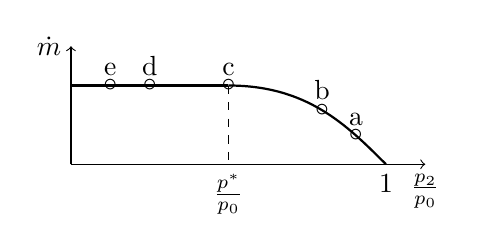
\begin{tikzpicture}
			\draw[->](0,0)--(4.5,0) node[anchor=north]{$\frac{p_2}{p_0}$};
			\draw[->](0,0)--(0,1.5) node[anchor=east]{$\dot{m}$};
			\draw[thick](0,1)--
			node[near start]{$\circ$}
			node[near start,above]{e}
			node[midway]{$\circ$}
			node[midway,above]{d}
			(2,1)
			node{$\circ$}
			node[above]{c};
			\draw[thick](2,1) ..controls (3,1) and (3.5,0.5).. 
			node[midway]{$\circ$}
			node[midway,above]{b}
			node[near end]{$\circ$}
			node[near end,above]{a}
			(4,0)
			node[below]{1};
			\draw[dashed](2,1)--(2,0)
			node[below]{$\frac{p^*}{p_0}$};
		\end{tikzpicture}
		\par\end{center}
	


\subsection{Tobera convergente-divergente}

\begin{center}
	\includegraphics[width=0.7\linewidth]{TeX_files/chapter11-Compresible/tobera_convergente_divergente}
\end{center}

	
	Si el flujo es supersónico (está bloqueado) pero las condiciones en
	la salida no son las adecuadas para mantenerlo en este estado, el
	flujo salta de forma irreversible, con una onda de choque, a un estado
	subsónico que le permita llegar al exterior con las condiciones.
	
	Las condiciones para la que el flujo se mantiene supersónico sin crear
	una onda de choque (caso $g$) se dicen que son las \emph{condiciones
		de diseño de la tobera}.
	
	\begin{center}
		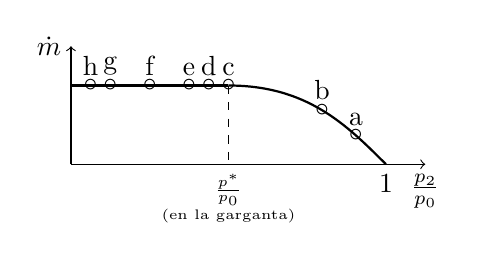
\begin{tikzpicture}
			\draw[->](0,0)--(4.5,0) node[anchor=north]{$\frac{p_2}{p_0}$};
			\draw[->](0,0)--(0,1.5) node[anchor=east]{$\dot{m}$};
			\draw[thick](0,1)--
			node[very near start]{$\circ$}
			node[very near start,above]{h}
			node[near start]{$\circ$}
			node[near start,above]{g}
			node[midway]{$\circ$}
			node[midway,above]{f}
			node[near end]{$\circ$}
			node[near end,above]{e}
			node[very near end]{$\circ$}
			node[very near end,above]{d}
			(2,1)
			node{$\circ$}
			node[above]{c};
			\draw[thick](2,1) ..controls (3,1) and (3.5,0.5).. 
			node[midway]{$\circ$}
			node[midway,above]{b}
			node[near end]{$\circ$}
			node[near end,above]{a}
			(4,0)
			node[below]{1};
			\draw[dashed](2,1)--(2,0)
			node[below]{$\binom{\frac{p^*}{p_0}}{\textrm{\tiny{(en la garganta)}}}$};
		\end{tikzpicture}
		\par\end{center}
	
	
	Si la presión en la descarga ($p_{2}$) es inferior a la presión de
	diseño de la tobera ($p^{*}$para la tobera convergente y $p_{g}$
	para la convergente-divergente) el flujo no puede bajar su presión
	mediante ondas de choque, ya que esto implicaría una disminución de
	la entropía. El flujo se expande en este caso mediante una \emph{expansión
		de Prandtl-Meyer}. Es una compleja expansión supersónica isentrópica
	en forma de abanico, en la que $\ma$ aumenta, y la presión disminuye.

	
	\textbf{Ejemplo:}
		En un tanque hay aire con una presión de $\unit[300]{kPa}$y una
		temperatura de $\unit[20]{^{\circ}C}$. A través de un conducto convergente,
		con un diámetro final de $\unit[4]{cm}$, se descarga el aire en otro
		tanque en el que la presión es de $\unit[200]{kPa}$. Considerando
		$\gamma=1.4$, queremos calcular el flujo másico.
		
		La presión para la cual obtendríamos flujo sónico y, por lo tanto
		bloqueado, es
		\[
		p^{*}=p_{0}\left(\frac{2}{\gamma+1}\right)^{\frac{\gamma}{\gamma-1}}=0.5283p_{0}=\unit[158.48]{kPa}
		\]
		
		La presión que tenemos en la salida es mayor, por lo que el flujo
		no se bloquea.

		El flujo másico lo calculamos mediante las condiciones en la salida,
		suponiendo flujo isentrópico,{\footnotesize{}
			\[
			\dot{m}=\rho_{2}u_{2}S_{2}=p_{2}\sqrt{\frac{\gamma}{rT_{2}}}\ma_{2}S_{2}=p_{0}\sqrt{\frac{\gamma}{rT_{0}}}\ma_{2}S_{2}\left[1+\frac{\gamma-1}{2}\ma^{2}\right]^{\frac{\gamma+1}{2\left(1-\gamma\right)}}
			\]
		}{\footnotesize\par}
		
		Para calcular el número de Mach en la salida
		\[
		\frac{p_{0}}{p_{2}}=\left[1+\frac{\gamma-1}{2}\ma_{2}^{2}\right]^{\frac{\gamma}{\gamma-1}}\;\Rightarrow\;\ma_{2}=0.784
		\]
		
		y el flujo es entonces $\unitfrac[0.852]{kg}{s}$.
		
		Si la presión en el recipiente de descarga estuviese por debajo de
		$\unit[158.48]{kPa}$, el flujo másico sería máximo,
		
		{\footnotesize{}
			\[
			\dot{m}_{\textrm{max}}=\rho^{*}u^{*}S^{*}=p^{*}\sqrt{\frac{\gamma}{rT^{*}}}S^{*}=p_{0}\sqrt{\frac{\gamma}{rT_{0}}}S_{2}\left[\frac{\gamma+1}{2}\right]^{\frac{\gamma+1}{2\left(1-\gamma\right)}}=\unitfrac[0.890]{kg}{s}
			\]
		}{\footnotesize\par}
		
		y es independiente del valor de $p_{2}$.


\section{El cono de Mach}

	
	\begin{center}
		\begin{animateinline}[poster=last,controls]{8}
			\multiframe{80}{rt=0+0.05,rv=0+0,rc=1+0,rperiod=0.2+0}{
				\begin{tikzpicture}[>=stealth]
					\clip (-6,-3) rectangle (0.5,3);
					\draw(-7,0) -- (1,0);
					\node at (-2.5,-2.5) {Ma=0};
					\fill[black](-\rv*\rt,0) circle (0.05);
					\foreach \w in {0,1,...,19}{
						\pgfmathparse{max(\rc*\rt-\rc*\rperiod*\w,0)}
						\let\radius\pgfmathresult
						\draw (-\rv*\rperiod*\w,0) circle(\radius);
						}
				\end{tikzpicture}
			}
			
		\end{animateinline}
		\par\end{center}
	

	
	\begin{center}
		\begin{animateinline}[poster=last,controls]{8}
			\multiframe{80}{rt=0+0.05,rv=0.5+0,rc=1+0,rperiod=0.2+0}{
				\begin{tikzpicture}[>=stealth]
					\clip (-6,-3) rectangle (0.5,3);
					\draw(-7,0) -- (1,0);
					\node at (-2.5,-2.5) {Ma=0.5};
					\fill[black](-\rv*\rt,0) circle (0.05);
					\foreach \w in {0,1,...,19}{
						\pgfmathparse{max(\rc*\rt-\rc*\rperiod*\w,0)}
						\let\radius\pgfmathresult
						\draw (-\rv*\rperiod*\w,0) circle(\radius);
						
					}
				\end{tikzpicture}
			}
			
		\end{animateinline}
		\par\end{center}
	

	
	\begin{center}
		\begin{animateinline}[poster=last,controls]{8}
			\multiframe{80}{rt=0+0.05,rv=1+0,rc=1+0,rperiod=0.2+0}{
				\begin{tikzpicture}[>=stealth]
					\clip (-6,-3) rectangle (0.5,3);
					\draw(-7,0) -- (1,0);
					\node at (-2.5,-2.5) {Ma=1};
					\fill[black](-\rv*\rt,0) circle (0.05);
					\foreach \w in {0,1,...,19}{
						\pgfmathparse{max(\rc*\rt-\rc*\rperiod*\w,0)}
						\let\radius\pgfmathresult
						\draw (-\rv*\rperiod*\w,0) circle(\radius);
						
					}
				\end{tikzpicture}
			}
			
		\end{animateinline}
		\par\end{center}
	

	
	\begin{center}
		\begin{animateinline}[poster=last,controls]{8}
			\multiframe{80}{rt=0+0.05,rv=2.5+0,rc=1+0,rperiod=0.2+0}{
				\begin{tikzpicture}[>=stealth]
					\clip (-6,-3) rectangle (0.5,3);
					\draw(-7,0) -- (1,0);
					\node at (-2.5,-2.5) {Ma=2.5};
					\fill[black](-\rv*\rt,0) circle (0.05);
					\foreach \w in {0,1,...,19}{
						\pgfmathparse{max(\rc*\rt-\rc*\rperiod*\w,0)}
						\let\radius\pgfmathresult
						\draw (-\rv*\rperiod*\w,0) circle(\radius);
						
					}
				\end{tikzpicture}
			}
			
		\end{animateinline}
		\par\end{center}
	
	
	En la figura, tomada del White\cite{White2008}, una fuente sonora
	se mueve con una velocidad $U$, que puede ser menor, igual o mayor
	que la velocidad del sonido (en la figura, denominada $a$)
	
	\begin{center}
		\includegraphics[height=5cm]{TeX_files/chapter11-Compresible/cono_de_Mach}
		\par\end{center}
	
	
	Si la velocidad del objeto es mayor que la del sonido, se forma el
	denominado \emph{cono de Mach }(hay que considerar que es tridimensional).
	Lo que hay fuera del cono en un cierto instante es la zona de silencio.
	Un objeto en esta zona no es capaz de ``oir'' la fuente de sonido
	hasta que la onda de Mach no le alcance.
	\textbf{Actividad 1:}
		Un micrófono está situado en la cima de una colina, y ``oye''
		un objeto supersónico cuando éste se encuentra a 500 m en horizontal
		de su posición. Sabiendo que el objeto vuela a 850 m/s y que la temperatura
		ambiente es de 288 K, calcular la altura a la que vuela el objeto
		por encima del micrófono.


\section{Onda de choque oblicua}

	
	En ocasiones un flujo supersónico es desviado por un objeto. Se crea
	entonces una onda de choque oblicua que forma un ángulo $\beta$ con
	el flujo, que es más o menos arbitrario. El flujo es entonces deflectado
	un ángulo $\theta$ que es función de $\beta$ y de las condiciones
	aguas arriba. 
	
	El flujo antes de la onda de choque es supersónico. Después puede
	ser subsónico, sónico o supersónico, dependiendo de las condiciones.
	
	Aplicando la conservación de masa, cantidad de movimiento y energía
	en un VC que encierra únicamente un área $S$ de la onda de choque,
	obtenemos
	
	\[
	\begin{array}{cc}
		\rho_{1}u_{n1}=\rho_{2}u_{n2} & p_{1}-p_{2}=\rho_{2}u_{n2}^{2}-\rho_{1}u_{n1}^{2}\\
		h_{0}=h_{1}+\frac{1}{2}u_{1}^{2}=h_{2}+\frac{1}{2}u_{2}^{2} & 0=\rho_{1}u_{n1}(u_{t2}-u_{t1})
	\end{array}
	\]
	
	
	\begin{center}
		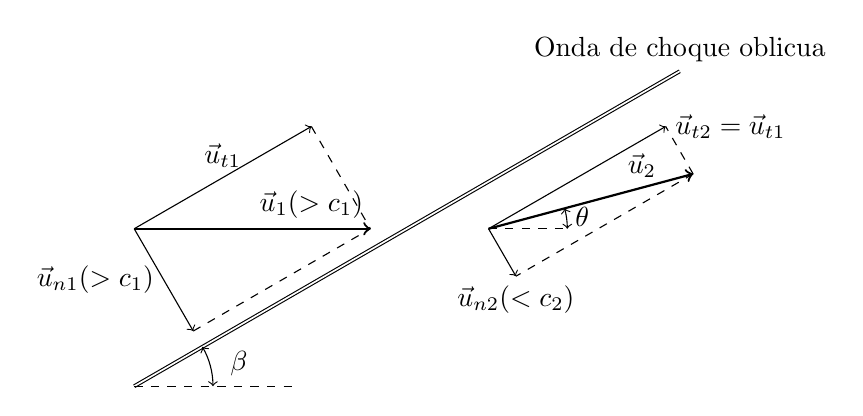
\begin{tikzpicture}
			\draw[double](0,0)--(30:8) node[above]{Onda de choque oblicua};
			\draw[thick,->](0,2) -- node[near end,above]{$\vec{u}_1(>c_1)$} (3,2) ;
			\draw[->](0,2)-- node[midway,left]{$\vec{u}_{n1}(>c_1)$} +(-60:1.5);
			\draw[->](0,2)-- node[midway,above]{$\vec{u}_{t1}$} +(30:2.598);
			\draw[dashed](0,2)++(30:2.598)--(3,2);
			\draw[dashed](0,2)++(-60:1.5)--(3,2);
			\draw[dashed](0,0)--(2,0);
			\draw[<->](1,0)  arc (0:30:1) ;
			\draw(15:1.1) node[right=1pt]{$\beta$};
			%
			\draw[thick,->](4.5,2)-- node[near end,above]{$\vec{u}_2$} +(15:2.690);
			\draw[->](4.5,2)--  +(30:2.598) node[right]{$\vec{u}_{t2}=\vec{u}_{t1}$};
			\draw[->](4.5,2)--  +(-60:0.696) node[below]{$\vec{u}_{n2}(<c_2)$};
			\draw[dashed](4.5,2)+(15:2.690)--+(-60:0.696);
			\draw[dashed](4.5,2)+(15:2.690)--+(30:2.598);
			\draw[dashed](4.5,2)--+(0:1);
			\draw[<->](4.5,2)+(0:1) arc(0:15:1);
			\draw(4.5,2)+(7.5:1.2) node{$\theta$};
		\end{tikzpicture}
		\par\end{center}
	
	
	La única diferencia entre estas ecuaciones y las relativas a la onda
	de choque normal es que se añade una velocidad tangencial, que és
	idéntica a ambos lados de la onda, $u_{t1}=u_{t2}=u_{t}$, y cuyo
	único efecto es aumentar en $\frac{1}{2}u_{t}^{2}$ la energía.
	
	Por lo demás són idénticas, con las velocidades normales $u_{n1}$
	y $u_{n2}$ en los papeles de velocidades en la onda de choque normal. 
	
	Lo único que hay que hacer es definir un \emph{número de Mach normal},
	
\begin{equation}
		\ma_{n}=\frac{u_{n}}{c}
\end{equation}
	
	
	y las relaciones que obtuvimos para ondas de choque normales se escriben
	ahora como
	
\begin{equation}		\frac{p_{2}}{p_{1}}=\frac{2\gamma\ma_{n1}^{2}-(\gamma-1)}{\gamma+1}
\end{equation}
	
	
	
	\begin{equation}
		\ma_{n2}^{2}=\frac{\left(\gamma-1\right)\ma_{n1}^{2}+2}{2\gamma\ma_{n1}^{2}-(\gamma-1)}
	\end{equation}
	
	

	
	
	\begin{equation}
		\frac{\rho_{2}}{\rho_{1}}=\frac{u_{n1}}{u_{n2}}=\frac{\left(\gamma+1\right)\ma_{n1}^{2}}{\left(\gamma-1\right)\ma_{n1}^{2}+2}=\frac{\tan\beta}{\tan\left(\beta-\theta\right)}
	\end{equation}
	
	
	
	\begin{equation}
		\frac{T_{2}}{T_{1}}=\left[2+\left(\gamma-1\right)\ma_{n1}^{2}\right]\frac{2\gamma\ma_{n1}^{2}-\left(\gamma-1\right)}{\left(\gamma+1\right)^{2}\ma_{n1}^{2}}
	\end{equation}
	
	
	
	\begin{equation}
		\frac{p_{02}}{p_{01}}=\frac{\rho_{02}}{\rho_{01}}=\left[\frac{\left(\gamma+1\right)^{2}\ma_{n1}^{2}}{2+\left(\gamma-1\right)\ma_{n1}^{2}}\right]^{\frac{\gamma}{\gamma-1}}\left[\frac{\gamma+1}{2\gamma\ma_{n1}^{2}-\left(\gamma-1\right)}\right]^{\frac{1}{\gamma-1}}
	\end{equation}
	
	
	En la siguiente gráfica se ha representado $\ma_{n1}$ en función
	de $\beta$ para diferentes valores de $\theta$, usando la primera
	de las expresiones dadas. 

	
	\begin{center}
		\includegraphics[width=0.7\textwidth]{TeX_files/chapter11-Compresible/oblicuas}
		\par\end{center}
	
	
	Calculemos el ángulo de deflección $\theta$. De la figura de la onda
	de choque oblicua se puede deducir por trigonometría que 
	
	
\begin{equation}
		\theta=\arctan\frac{u_{t}}{u_{n2}}-\arctan\frac{u_{t}}{u_{n1}}
\end{equation}
	
	
	Podemos ahora calcular el valor de $u_{t}$ para el cuál el ángulo
	de deflección en máximo,
	
	\begin{equation}
		\frac{\dif\theta}{\dif u_{t}}=0\;\Rightarrow\;\frac{u_{t}}{u_{n1}}=\sqrt{\frac{u_{n2}}{u_{n1}}};\frac{u_{t}}{u_{n2}}=\sqrt{\frac{u_{n1}}{u_{n2}}}
	\end{equation}
	
	
	
	\begin{equation}
		\Rightarrow\;\theta_{\textrm{max}}=\arctan\sqrt{\frac{u_{n1}}{u_{n2}}}-\arctan\sqrt{\frac{u_{n2}}{u_{n1}}}
	\end{equation}
	
	
	Esto limita bastante los posibles valores de deflección
	\textbf{Ejemplo:}
		Para $\ma_{n1}=5.0$ y $\gamma=1.4$, se tiene $\frac{u_{n1}}{u_{n2}}=5$
		y el ángulo de deflección máxima es $\theta_{\textrm{max}}=41.81^{\circ}$


	
	\textbf{Actividad 2:} Calcular el ángulo de deflección máximo para un flujo incidente con
		$\ma_{n1}\rightarrow\infty$.

	Para una $\vec{u}_{1}$, $c_{1}$ y $\gamma$ dadas, es posible resolver
	las ecuaciones para encontrar todos los valores posibles de $\vec{u}_{2}=u_{2x}\vec{\imath}+u_{2y}\vec{\jmath}$.
	El resultado es una \emph{hodografía.}
	
	\begin{center}
		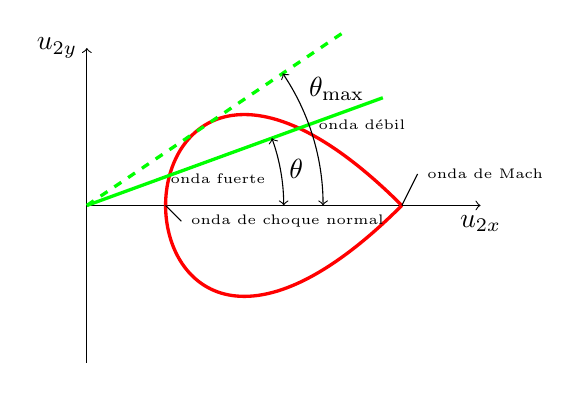
\begin{tikzpicture}
			\draw[->](0,0)--(5,0) node[below]{$u_{2x}$};
			\draw[->](0,-2)--(0,2) node[left]{$u_{2y}$};
			\draw[color=red,very thick] (4,0) ..controls (2,2) and (1,1) ..(1,0);
			\draw[color=red,very thick] (4,0) ..controls (2,-2) and (1,-1) ..(1,0);
			\draw[color=green,very thick] (0,0) -- (20:4);
			\draw(0,0)+(20:1) node[right]{\tiny onda fuerte};
			\draw(0,0)+(20:3) node[right]{\tiny onda débil};
			\draw[color=green,very thick,dashed] (0,0) -- (34:4);
			\draw[<->](2.5,0)arc(0:20:2.5);
			\draw(0,0)+(10:2.7) node{$\theta$};
			\draw[<->](3,0)arc(0:34:3);
			\draw(0,0)+(25:3.5) node{$\theta_{\textrm{max}}$};
			\draw(4,0)--(4.2,0.4) node[right]{\tiny onda de Mach};
			\draw(1,0)--(1.2,-0.2) node[right]{\tiny onda de choque normal};
		\end{tikzpicture}
		\par\end{center}
	




\backmatter
% bibliography, glossary and index would go here.

\nocite{*}
\printbibliography

\end{document}